% Gelfand seminar notes, 1969-70 and 1970-71: source pages P000282-P000360.
% English translation (AI-made, checked against the scans), cut page by page from the cumulative working reader A4-reader-chapters01-28-first1282-separated-diplomatic-r2.
% \SourcePage{GELFAND-Pnnnnnn}{label} starts a scanned page; the second argument is the number written
% on the page, if any. Editorial notes give the page, a label and the transcriber's remark; \Unclear
% marks a doubtful reading.
\SourcePage{GELFAND-P000282}{unlabelled}
\GelfandFitDiagram{
\begin{tikzpicture}[x=1mm, y=1mm]
\draw[line width=.45pt] (0,0) ..controls(2,3)and(3,3)..(2,0) ..controls(1,-2)and(-1,-2)..(0,0);
\draw[line width=.45pt] (2,0) ..controls(4,3)and(5,2)..(4,0) ..controls(3,-1)and(2,-1)..(2,0);
\draw[line width=.45pt] (-.5,1.5)--(5,1.2);
\end{tikzpicture}}

\Unclear{GELFAND-P000282}{cancelled-before-heading}{Two small crossed-out loop-shaped signs above and to the left of the surname. Possible reading: В.; undetermined.}
\end{GelfandAdjacentEvidence}


\underline{\underline{Buchstaber.}}

Manifolds of the homot. type of a torus are divided by $h$-cobordisms into a finite number of classes

\underline{\underline{Problem:}} to show that in $\forall$ class there is a finite number

Next, the simplest films are classified by Morse modifications.

\begin{center}\GelfandFitDiagram{\begin{tikzpicture}[x=1mm, y=1mm]
\draw[line width=.6pt] (-20,0)--(-3,0);
\fill (0,0) circle[radius=.45mm];
\draw[line width=.6pt] (3,0)--(20,0);
\draw[line width=.35pt] (47,-6) ..controls(53,-6)and(57,-5.5)..(63,-6);
\end{tikzpicture}}\end{center}

\hfill\GelfandFitDiagram{\begin{tikzpicture}[x=1mm, y=1mm]
\draw[line width=.45pt] (0,0)--(2,0);
\draw[line width=.45pt] (0,-5)--(2,-5.2);
\end{tikzpicture}}





\begin{GelfandAdjacentEvidence}{GELFAND-P000282}{2}
\hfill\GelfandFitDiagram{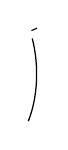
\begin{tikzpicture}[x=1mm, y=1mm]
\draw[line width=.45pt] (.1,5.5) ..controls(1,2)and(.8,-2)..(-.4,-5);
\draw[line width=.4pt] (0,6.5)--(.7,6.8);
\end{tikzpicture}}

\Unclear{GELFAND-P000282}{bottom-right-mark}{At bottom right, a curved vertical stroke with a separate short mark above it: ) / 1. The reading is undetermined.}
\end{GelfandAdjacentEvidence}




\Needspace{7\baselineskip}
\SourcePage{GELFAND-P000283}{unlabelled}
\textbf{15.9.69 yr.}

\underline{\underline{B. Vainberg}} on results of Hörmander. (see Vishik seminar). on singularities of fund. sol.

General sol. of homog. eqn.: (homog. polynomial)

\begin{equation*}\int_{P (\xi)=0}f[(x,\xi)]A (\xi)\, d\xi\qquad\text{(Borovikov)}\end{equation*}

$f, A$ — arbitrary functions.

Singularities in the homog. case are described by Borovikov.

For example:

\begin{GelfandAdjacentEvidence}{GELFAND-P000283}{1}
\begin{equation*}\int_{P (\xi)=0}\frac{(x\cdot\xi)^\lambda}{\Gamma (\lambda+1)}A (\xi)\, d\xi\end{equation*}

\Unclear{GELFAND-P000283}{borovikov-numerator}{A short crossed stroke between $x$ and $\xi$: dot /plus /comma. The parentheses and superscript $\lambda$ are visible; the dotted reading is undetermined.}
\end{GelfandAdjacentEvidence}


— proposal of Borovikov.

\begin{center}\GelfandFitDiagram{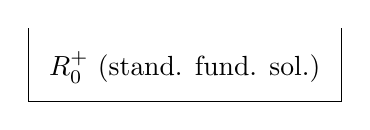
\begin{tikzpicture}
\node (f) {$R_0^+$ (stand. fund. sol.)};
\draw ([xshift=-4pt,yshift=5pt]f.north west)--([xshift=-4pt,yshift=-3pt]f.south west)--([xshift=4pt,yshift=-3pt]f.south east)--([xshift=4pt,yshift=5pt]f.north east);
\end{tikzpicture}}\end{center}





Grushin:

\begin{equation*}\sum_j\int\frac{\alpha_j (\xi)e^{i (x,\xi)}}{P (\xi)\pm i0}\, d\xi\end{equation*}

$\alpha_j$ — partition of unity on the sphere.





\underline{The Bernstein problem is solved.}

\begin{GelfandAdjacentEvidence}{GELFAND-P000283}{2}
\begin{equation*}\left\{\begin{gathered}
z=f (x_1,\ldots, x_{n-1})\text{ — min. surf.}\\
(x\text{-arbitrary})\ \Longrightarrow\ \text{it is a plane.}
\end{gathered}\right\}\end{equation*}

\Unclear{GELFAND-P000283}{graph-variable-index}{The final variable index: $n-1$ /$n+1$; the short strokes merge. The reading is undetermined.}
\end{GelfandAdjacentEvidence}


true for $n\leq8$; for $n\geq9$ \underline{\underline{false}}.

\GelfandFitDiagram{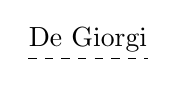
\begin{tikzpicture}[baseline=(n.base)]\node[inner sep=0pt](n){De Giorgi};\draw[dashed]([yshift=-2pt]n.south west)--([yshift=-2pt]n.south east);\end{tikzpicture}}, \GelfandFitDiagram{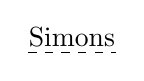
\begin{tikzpicture}[baseline=(n.base)]\node[inner sep=0pt](n){Simons};\draw[dashed]([yshift=-2pt]n.south west)--([yshift=-2pt]n.south east);\end{tikzpicture}} and \GelfandFitDiagram{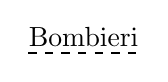
\begin{tikzpicture}[baseline=(n.base)]\node[inner sep=0pt](n){Bombieri};\draw[dashed]([yshift=-2pt]n.south west)--([yshift=-2pt]n.south east);\end{tikzpicture}}.

\GelfandFitDiagram{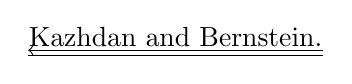
\begin{tikzpicture}[baseline=(k.base)]
\node[inner sep=0pt](k){Kazhdan and Bernstein.};
\draw[<-]([yshift=-1pt]k.south west)--([yshift=-1pt]k.south east);
\draw([yshift=-3pt]k.south west)--([yshift=-3pt]k.south east);
\end{tikzpicture}}

\begin{GelfandAdjacentEvidence}{GELFAND-P000283}{3}
Convergence of the spectrum as the domains expand.





\SourceFigure{GELFAND-P000283}{nested-domains}{\par\smallskip\centering{\color{black}\GelfandFitDiagram{\begin{minipage}{68mm}\raggedright \GelfandFitDiagram{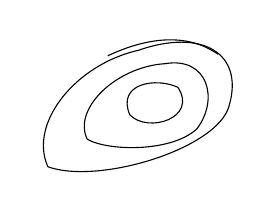
\begin{tikzpicture}
\draw (0,0) .. controls (-0.25,0.55) and (0.35,1.30) .. (1.15,1.48)
 .. controls (1.95,1.76) and (2.50,1.45) .. (2.30,0.77)
 .. controls (2.15,0.23) and (0.65,-0.23) .. (0,0);
\draw (0.50,0.35) .. controls (0.31,0.73) and (0.86,1.27) .. (1.49,1.31)
 .. controls (2.03,1.40) and (2.18,0.86) .. (1.89,0.48)
 .. controls (1.56,0.18) and (0.76,0.20) .. (0.50,0.35);
\draw (1.04,0.66) .. controls (0.87,1.06) and (1.37,1.14) .. (1.65,1.01)
 .. controls (1.91,0.62) and (1.27,0.42) .. (1.04,0.66);
\draw (0.76,1.41) .. controls (1.25,1.64) and (1.76,1.71) .. (2.16,1.43);
\end{tikzpicture}}\end{minipage}}}\par\smallskip }
\end{GelfandAdjacentEvidence}


$A$ — self-adj. op. on the manifold $X$.

$\Lambda\subset R$.

[Below $\Lambda$:] \uwave{interval}.

\uwave{The continuous functions contained in $E_\Lambda$ are dense in it.}

(required) — so for elliptic op.

$x_0\longrightarrow$ a Plancherel measure on the spectrum of $A$.

\begin{GelfandAdjacentEvidence}{GELFAND-P000283}{4}
\begin{equation*}M_{x_0}(\Lambda)=
\max_{\substack{f\text{-continuous in }E_\lambda,\ \|f\|=1\\
\text{(over all of }X\text{)}}}|f (x_0)|^2.\end{equation*}

\Unclear{GELFAND-P000283}{spectral-subscript}{Below $\max$: $E_\lambda$; possibly $E_\Lambda$. Above are $E_\Lambda$ and $M_{x_0}(\Lambda)$; the cases have not been made uniform.}
\end{GelfandAdjacentEvidence}


[At right:] This is a measure (possibly infinite).



\Needspace{7\baselineskip}
\SourcePage{GELFAND-P000284}{53}
$K_\Lambda (x, y)$ — the kernel of $E_\Lambda$.

\begin{flushright}\GelfandFitDiagram{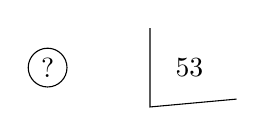
\begin{tikzpicture}[x=1mm, y=1mm]
\node[draw, circle, inner sep=2pt](q)at (-18,0){?};
\node at (0,0){$53$};
\draw(-5,5)--(-5,-5)--(6,-4);
\end{tikzpicture}}\end{flushright}
\begin{center}\GelfandFitDiagram{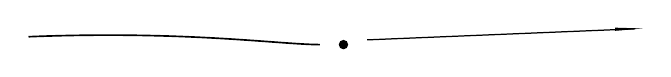
\begin{tikzpicture}[x=1mm, y=1mm]
\draw[line width=.6pt](-40,0)..controls(-20,.8)and(-8,-1)..(-3,-1);
\fill(0,-1)circle[radius=.6mm];
\draw[line width=.45pt](3,-.4)--(37,1);
\fill(34.5,.75)--(38,1.05)--(34.5,1.15)--cycle;
\end{tikzpicture}}\end{center}





\underline{Kazhdan.} M. Artin in the Bourbaki seminar.

\begin{equation*}f_i (x_1,\ldots, x_n)=0,\qquad1\leq i\leq k.\end{equation*}

$f_i$ — convergent power series.

\begin{GelfandAdjacentEvidence}{GELFAND-P000284}{1}
When does a sol. exist $\psi_j (t_1,\ldots, t_\tau)$

\Unclear{GELFAND-P000284}{artin-solution-parameters}{The function letter: $\psi$ /$Y$; the final index: $\tau$ /$r$. The reading is undetermined.}
\end{GelfandAdjacentEvidence}


\underline{Answer:} if and only if there is a sol. in formal power series.

(arbitrarily close to the formal one)

[Below the parenthesis:] can be completed

\begin{center}\GelfandFitDiagram{\begin{tikzpicture}[x=1mm, y=1mm]
\draw[line width=.55pt](-20,0)--(-3,0);
\fill(0,0)circle[radius=.6mm];
\draw[line width=.55pt](3,0)--(20,0);
\end{tikzpicture}}\end{center}

\textbf{22.9.69 yr.}

\begin{GelfandAdjacentEvidence}{GELFAND-P000284}{2}
\underline{Fikera} \underline{on} \underline{unilateral} \underline{bound.} \underline{problems.}





\SourceFigure{GELFAND-P000284}{elastic-body}{\par\smallskip\centering{\color{black}\GelfandFitDiagram{\begin{minipage}{68mm}\raggedright \GelfandFitDiagram{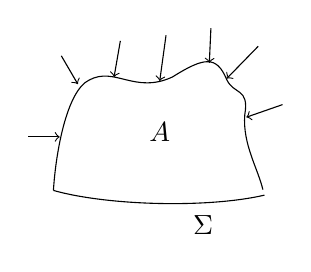
\begin{tikzpicture}
\draw (0,0.08) .. controls (0.03,0.57) and (0.17,1.34) .. (0.45,1.48)
 .. controls (0.78,1.66) and (1.03,1.30) .. (1.51,1.52)
 .. controls (1.91,1.77) and (2.07,1.80) .. (2.20,1.49)
 .. controls (2.29,1.29) and (2.49,1.39) .. (2.43,1.04)
 .. controls (2.40,0.67) and (2.60,0.35) .. (2.66,0.09);
\draw (0,0.08) .. controls (0.67,-0.11) and (1.94,-0.15) .. (2.68,0.02);
\draw[->] (-0.32,0.76) -- (0.08,0.76);
\draw[->] (0.10,1.79) -- (0.31,1.43);
\draw[->] (0.85,1.98) -- (0.77,1.52);
\draw[->] (1.43,2.05) -- (1.35,1.47);
\draw[->] (2.00,2.14) -- (1.98,1.70);
\draw[->] (2.60,1.91) -- (2.20,1.50);
\draw[->] (2.91,1.17) -- (2.45,1.01);
\node at (1.35,0.82) {$A$};
\node at (1.90,-0.36) {$\Sigma$};
\end{tikzpicture}}\end{minipage}}}\par\smallskip }
\end{GelfandAdjacentEvidence}


An elastic body on a surface $\Sigma$ rigid and frictionless.

And the stress tensor $\equiv0$.

$A$ — natural volume of the body.

On the free part of the boundary, a force \GelfandFitDiagram{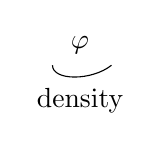
\begin{tikzpicture}[baseline=(p.base)]
\node (p)at (0,0){$\varphi$};
\draw(-.35,-.25)..controls(-.35,-.45)and(.15,-.45)..(.4,-.25);
\node at (0,-.7){density};
\end{tikzpicture}} on $\partial A-\Sigma=\Sigma^*$.





Inside there are also certain forces $f$ — volume forces.

Let the body move to a position of equil.

\begin{GelfandAdjacentEvidence}{GELFAND-P000284}{3}
It may separate from $\Sigma$.





\Unclear{GELFAND-P000284}{detachment-figure}{Contact is visible at the left. At the right, overlapping strokes and a narrow light strip; exact contact or separation and the length of contact are undetermined. There are no labels or arrows.\par\smallskip\centering{\color{black}\GelfandFitDiagram{\begin{minipage}{68mm}\raggedright \GelfandFitDiagram{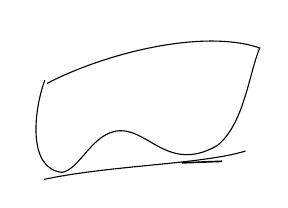
\begin{tikzpicture}
\draw (.14,1.16)..controls(.85,1.53)and(2.10,1.86)..(2.84,1.61)
 ..controls(2.70,1.27)and(2.64,.64)..(2.30,.37)
 ..controls(1.66,.00)and(1.40,.64)..(1.00,.55)
 ..controls(.70,.49)and(.54,.06)..(.33,.03)
 ..controls(-.10,.07)and(-.04,.78)..(.11,1.20);
\draw (.10,-.06)..controls(.94,.12)and(2.10,.13)..(2.66,.30);
\draw[line width=.6pt](1.85,.15)--(2.36,.17);
\end{tikzpicture}}\end{minipage}}}\par\smallskip }
\end{GelfandAdjacentEvidence}


This is an analytic problem (formulation A. Signorini, 1959)

$\sigma_{ik}$ — the stress tensor.

Inside the body

[Crossed out:] \GelfandFitDiagram{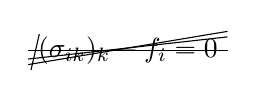
\begin{tikzpicture}[baseline=(c.base)]
\node (c){$(\sigma_{ik})_k-f_i=0$};
\draw(c.west)--(c.east);
\draw([yshift=-3pt]c.west)--([yshift=5pt]c.east);
\draw([yshift=-5pt]c.west)--([yshift=7pt]c.east);
\draw([xshift=1pt,yshift=-7pt]c.west)--([xshift=4pt,yshift=6pt]c.west);
\end{tikzpicture}}





[Written at the right:]

\begin{equation*}\sigma_{ik/k}-f_i=0.\end{equation*}

$(\operatorname{div}\sigma=f)$.

\begin{equation*}\sigma_{ik}\nu_k-\varphi_i=0.\end{equation*}

— bound. conditions.

\begin{GelfandAdjacentEvidence}{GELFAND-P000284}{4}
($\nu$ — normal vector)

\Unclear{GELFAND-P000284}{normal-letter}{The normal sign in the formula and caption has the form $V$ /$\nu$; the choice of letter is not established from the shape alone.}
\end{GelfandAdjacentEvidence}




\Needspace{7\baselineskip}
\SourcePage{GELFAND-P000285}{unlabelled}
\GelfandFitDiagram{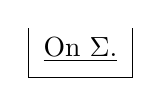
\begin{tikzpicture}[baseline=(s.base)]
\node (s){\underline{On $\Sigma$.}};
\draw([xshift=-2pt]s.north west)--([xshift=-2pt,yshift=-2pt]s.south west)--([xshift=2pt,yshift=-2pt]s.south east)--([xshift=2pt]s.north east);
\end{tikzpicture}}

$u_i$ — the displacement vector.

\begin{GelfandAdjacentEvidence}{GELFAND-P000285}{1}
\begin{center}\GelfandFitDiagram{\begin{tikzpicture}[x=1mm, y=1mm]
\node at (-29,18){Condition};
\node at (4,18){$u_i\nu_i=0\quad (\text{on }\Sigma)$};
\node at (-19,3){Normal reaction};
\node at (29,3){$\sigma_{ik}\nu_i\nu_k\geq0$};
\node at (29,-11){$\sigma_{ik}\nu_i\tau_k=0$};
\node[anchor=west, inner sep=0pt] at (62,-11){$\text{— tang. comp.}$};
\draw(-18,26)--(-18,11)--(9,8)--(9,-20)--(58,-20)--(58,-8);
\end{tikzpicture}}\end{center}

\Unclear{GELFAND-P000285}{contact-framing-normal}{The conditions are joined by an open stepped line. The normal sign has the form $\nu$ /$V$; the shape alone does not establish the letter.}
\end{GelfandAdjacentEvidence}


At a point of the free surface:

\begin{equation*}\begin{cases}
u_i\nu_i>0,\\
\sigma_{ik}\nu_i\nu_k=0,\\
\sigma_{ik}\nu_i\tau_k=0.
\end{cases}\end{equation*}

\textbf{But} it is unknown where which occurs.

We have not yet taken into account that the body is elastic.

\begin{center}\GelfandFitDiagram{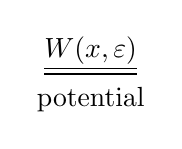
\begin{tikzpicture}
\node (p)at (0,0){$\underline{\underline{W (x,\varepsilon)}}$};
\node at (0,-.55){potential};
\end{tikzpicture}}\end{center}

\begin{equation*}\varepsilon=\{\varepsilon_{ik}\}\qquad\varepsilon_{ik}=2^{-1}(u_{i/k}+u_{k/i})\end{equation*}

\begin{center}Strain tensor.\end{center}





Relation:

\begin{equation*}\sigma_{ik}+W_{\varepsilon_{ik}}=0\qquad\text{on }A.\end{equation*}

Problem of exist. and uniqueness.

\begin{equation*}\begin{aligned}
I (u)={}&\int_A W[x,\varepsilon (u)]\, dx\\
&-\underbrace{\int_A f_i u_i\, dx}_{\text{work of }f}
-\underbrace{\int_\Sigma\varphi_i u_i\, d\Sigma}_{\text{work of }\varphi}.
\end{aligned}\end{equation*}

\begin{GelfandAdjacentEvidence}{GELFAND-P000285}{2}
(Total energy)

\Unclear{GELFAND-P000285}{energy-boundary-domain}{The first surface integral is written with $\Sigma$, without a star.}
\end{GelfandAdjacentEvidence}


\begin{GelfandAdjacentEvidence}{GELFAND-P000285}{3}
\uwave{In the class of admissible displacements $\mathcal W_\Sigma$.}

\Unclear{GELFAND-P000285}{admissible-class-letter}{The heavily retraced letter: $\mathcal W_\Sigma$ /$\mathcal U_\Sigma$; it is not made uniform with the model-class notation below.}
\end{GelfandAdjacentEvidence}


If a minimum exists in $C^1(\Sigma)$, then it is a solution.

\begin{GelfandAdjacentEvidence}{GELFAND-P000285}{4}
conversely, a solution is a $\min$.

\Unclear{GELFAND-P000285}{regularity-domain}{Written $C^1(\Sigma)$; there is no bar over $\Sigma$.}
\end{GelfandAdjacentEvidence}


But: in this class \GelfandFitDiagram{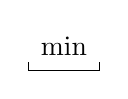
\begin{tikzpicture}[baseline=(m.base)]
\node (m){$\min$};
\draw([xshift=-1pt,yshift=1pt]m.south west)--([xshift=-1pt,yshift=-2pt]m.south west)--([xshift=1pt,yshift=-2pt]m.south east)--([xshift=1pt,yshift=1pt]m.south east);
\end{tikzpicture}} does not exist.





\begin{center}\GelfandFitDiagram{\begin{tikzpicture}[x=1mm, y=1mm]
\draw[line width=.55pt](-20,0)--(-3,0);
\fill(0,0)circle[radius=.35mm];
\draw[line width=.55pt](3,0)--(20,0);
\end{tikzpicture}}\end{center}

\begin{equation*}\begin{aligned}
I (u)={}&\frac12\int_A a_{nk}(x)u_{/n}u_{/k}\, dx\\
&-\int_A fu\, dx-\int_{\Sigma^*}\varphi u\, d\sigma.
\end{aligned}\end{equation*}

\begin{equation*}a_{nk}(x)\mu_n\mu_k\geq\rho_0\mu_n\mu_n.\end{equation*}

\begin{equation*}\mathcal U_\Sigma:\quad u|_\Sigma\geq0.\end{equation*}

\begin{GelfandAdjacentEvidence}{GELFAND-P000285}{5}
(Model problem)





\Unclear{GELFAND-P000285}{boundary-partition-figure}{The upper arc: $\Sigma^*$; at lower left: $\Sigma$. Two ringed junction marks; the left one is retraced, with an oblique stroke. Its role and an orientation of traversal are undetermined.\par\smallskip\centering{\color{black}\GelfandFitDiagram{\begin{minipage}{68mm}\raggedright \GelfandFitDiagram{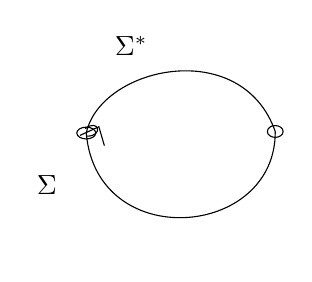
\begin{tikzpicture}
\draw(0,0)..controls(.18,.84)and(1.97,1.24)..(2.40,.02);
\draw(2.40,.02)..controls(2.41,-1.34)and(.13,-1.53)..(0,0);
\draw(0,0)ellipse[x radius=.12,y radius=.075];
\draw(2.40,.02)ellipse[x radius=.10,y radius=.075];
\draw(-.015,.055)..controls(.16,.19)and(.22,-.04)..(.01,-.04);
\draw(-.08,-.03)--(.16,.08)--(.23,-.16);
\node at (.57,1.10){$\Sigma^*$};
\node at (-.50,-.66){$\Sigma$};
\end{tikzpicture}}\end{minipage}}}\par\smallskip }
\end{GelfandAdjacentEvidence}




\Needspace{7\baselineskip}
\SourcePage{GELFAND-P000286}{54}
From this we obtain the problem.

\begin{center}\GelfandFitDiagram{\begin{tikzpicture}
\node (b){$u=0,\quad a\dfrac{\partial u}{\partial\lambda}\geq0$};
\draw[line width=.6pt](b.north west)--(b.north east)--(b.south east)--(b.south west)--cycle;
\draw([xshift=-2pt]b.west)..controls(b.north west)and(b.north east)..([xshift=2pt]b.east)..controls(b.south east)and(b.south west)..([xshift=-2pt]b.west);
\draw([yshift=-5pt]b.south west)--([yshift=-5pt]b.south east);
\draw([xshift=4pt,yshift=-1pt]b.south west)--([xshift=10pt,yshift=-5pt]b.south west);
\draw([xshift=16pt,yshift=-1pt]b.south west)--([xshift=22pt,yshift=-5pt]b.south west);
\draw([xshift=28pt,yshift=-1pt]b.south west)--([xshift=34pt,yshift=-5pt]b.south west);
\draw([xshift=40pt,yshift=-1pt]b.south west)--([xshift=46pt,yshift=-5pt]b.south west);
\draw([xshift=52pt,yshift=-1pt]b.south west)--([xshift=58pt,yshift=-5pt]b.south west);
\draw([xshift=64pt,yshift=-1pt]b.south west)--([xshift=70pt,yshift=-5pt]b.south west);
\draw([xshift=76pt,yshift=-1pt]b.south west)--([xshift=82pt,yshift=-5pt]b.south west);
\draw([xshift=88pt,yshift=-1pt]b.south west)--([xshift=94pt,yshift=-5pt]b.south west);
\end{tikzpicture}}
\quad\text{or}\quad
$\begin{cases}u>0,\\a\dfrac{\partial u}{\partial\lambda}=0.\end{cases}$
\end{center}

\begin{flushright}\GelfandFitDiagram{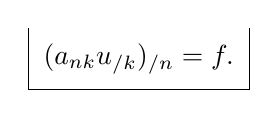
\begin{tikzpicture}[baseline=(f.base)]
\node (f){$(a_{nk}u_{/k})_{/n}=f. $};
\draw([xshift=-2pt,yshift=2pt]f.north west)--([xshift=-2pt,yshift=-2pt]f.south west)--([xshift=2pt,yshift=-2pt]f.south east)--([xshift=2pt,yshift=2pt]f.north east);
\end{tikzpicture}}\quad\GelfandFitDiagram{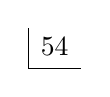
\begin{tikzpicture}\node (p){$54$};\draw([xshift=-1pt]p.north west)--([xshift=-1pt,yshift=-1pt]p.south west)--([xshift=1pt,yshift=-1pt]p.south east);\end{tikzpicture}}\end{flushright}





Necessary:

\begin{GelfandAdjacentEvidence}{GELFAND-P000286}{1}
\begin{equation*}\int_A f\, dx+\int_{\Sigma^*}\varphi\, d\Sigma\leq0.\end{equation*}

\Unclear{GELFAND-P000286}{first-integral-differential}{The first integral differential: $dx$ /$d\Sigma$; possibly $\Sigma$ is changed to $x$. The strokes overlap.}
\end{GelfandAdjacentEvidence}
\begin{GelfandAdjacentEvidence}{GELFAND-P000286}{2}


\Unclear{GELFAND-P000286}{first-integral-domain-overwrite}{The final $A$ below the first integral is traced over earlier strokes. A possible earlier $\Sigma$ is undetermined.}
\end{GelfandAdjacentEvidence}


Let $f\leq0$ on $A$ and $\varphi<0$ on $\Sigma^*$.

By the $\min$ principle, $u$ cannot have a min. in $A$.

There is no sol. in $\underline{\underline{C^1(\bar A)}}$.

\GelfandFitDiagram{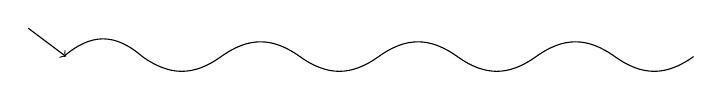
\begin{tikzpicture}
\draw[->](-.45,.36)--(.03,0);
\draw(0,0)..controls(.35,.30)and(.65,.30)..(1,0)..controls(1.35,-.25)and(1.65,-.25)..(2,0)
 ..controls(2.35,.25)and(2.65,.25)..(3,0)..controls(3.35,-.25)and(3.65,-.25)..(4,0)
 ..controls(4.35,.25)and(4.65,.25)..(5,0)..controls(5.35,-.25)and(5.65,-.25)..(6,0)
 ..controls(6.35,.25)and(6.65,.25)..(7,0)..controls(7.35,-.25)and(7.65,-.25)..(8,0);
\end{tikzpicture}}

(deduced from Green’s formula)

\uwave{an immediate contradiction — a discontinuity of the derivative is obtained.}





\GelfandFitDiagram{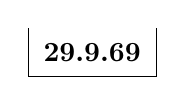
\begin{tikzpicture}[baseline=(f.base)]
\node (f){\textbf{29.9.69}};
\draw([xshift=-2pt,yshift=2pt]f.north west)--([xshift=-2pt,yshift=-2pt]f.south west)--([xshift=2pt,yshift=-2pt]f.south east)--([xshift=2pt,yshift=2pt]f.north east);
\end{tikzpicture}}

\underline{Kazhdan} \uwave{Formulation} of results of \uwave{M. Artin}. (1968).





\begin{GelfandAdjacentEvidence}{GELFAND-P000286}{3}
(in the USSR independently Pokornii and Rybkin)

\Unclear{GELFAND-P000286}{pokorny-surname}{The first surname: Pokornii /Pokornyi (Покорний /Покорный); the joined ending does not establish иorы.}
\end{GelfandAdjacentEvidence}


UMN, vol. 15, $N=4$ (1960) p. 169

and Melamed

Sib. math. journal

\begin{equation*}f_i (x_1,\ldots, x_k)=0,\qquad1\leq i\leq n.\end{equation*}

a collection of convergent power series (in a nbd. of 0

We try to find

\begin{center}\GelfandFitDiagram{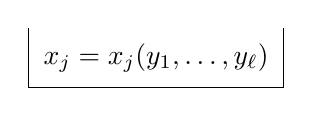
\begin{tikzpicture}[baseline=(f.base)]
\node (f){$x_j=x_j (y_1,\ldots, y_\ell)$};
\draw([xshift=-2pt,yshift=2pt]f.north west)--([xshift=-2pt,yshift=-2pt]f.south west)--([xshift=2pt,yshift=-2pt]f.south east)--([xshift=2pt,yshift=2pt]f.north east);
\end{tikzpicture}}\quad\GelfandFitDiagram{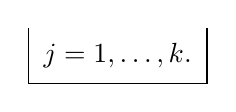
\begin{tikzpicture}[baseline=(f.base)]
\node (f){$j=1,\ldots, k. $};
\draw([xshift=-2pt,yshift=2pt]f.north west)--([xshift=-2pt,yshift=-2pt]f.south west)--([xshift=2pt,yshift=-2pt]f.south east)--([xshift=2pt,yshift=2pt]f.north east);
\end{tikzpicture}}\end{center}

so that the equalities hold upon substitution.

\underline{It is sufficient to find such functions in formal power series.}

\noindent\begin{tabular}{@{}p{.44\linewidth}|p{.48\linewidth}@{}}
\underline{Example.}
\begin{equation*}x_1^2-x_2^3=0\qquad\begin{aligned}x_1&=y^3,\\x_2&=y^2.\end{aligned}\end{equation*}
& Then a sol. in analytic functions will be found, arbitrarily close. (with any number of derivatives)\\\hline
\end{tabular}





the problem is handled by induction on the number of $x_j$.

and a more complicated ind.

\underline{Reformulation.}

These are equations of an analytic set and 2 rings

\begin{align*}
A&=C\{y_1,\ldots, y_\ell\}&&\text{convergent series.}\\
B&=C[[y_1,\ldots, y_\ell]]&&\text{formal series.}
\end{align*}

If \GelfandFitDiagram{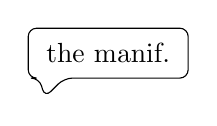
\begin{tikzpicture}[baseline=-.5ex]
\node (i){the manif.};
\draw[rounded corners=3pt]([xshift=-3pt,yshift=2pt]i.north west)--([xshift=3pt,yshift=2pt]i.north east)--([xshift=3pt,yshift=-2pt]i.south east)--([xshift=10pt,yshift=-2pt]i.south west)--([xshift=3pt,yshift=-9pt]i.south west)--([xshift=1pt,yshift=-2pt]i.south west)--([xshift=-3pt,yshift=-2pt]i.south west)--cycle;
\end{tikzpicture}} has a point with values in $B$, then there is also a point with values in $A$.







\Needspace{7\baselineskip}
\SourcePage{GELFAND-P000287}{unlabelled}
Induction also on conn. components. (\underline{\underline{their number}})

Irreduc. --- a subpiece has smaller dimension.

1) \uwave{If for irreduc. $\underset{\text{(of the given dim.)}}{\text{varieties}}$ proved, then also $\underset{\text{(given dim.)}}{\text{always proved.}}$}





\begin{GelfandAdjacentEvidence}{GELFAND-P000287}{1}
Choose eqns. lying in the ideal, \textbf{[crossed out: ?]} corresp. to this component.

\Unclear{GELFAND-P000287}{upper-cancelled-word}{A word between “ideal,” and “corresp.” is densely crossed out. Its initial stroke resembles Cyrillic “к”; the complete reading is undetermined.}
\end{GelfandAdjacentEvidence}


\begin{GelfandAdjacentEvidence}{GELFAND-P000287}{2}
\uwave{Adding eqns.} Consider a prime ideal.





\SourceFigure{GELFAND-P000287}{crossing-sketch}{\par\smallskip\centering{\color{black}\GelfandFitDiagram{\begin{minipage}{68mm}\raggedright \GelfandFitDiagram{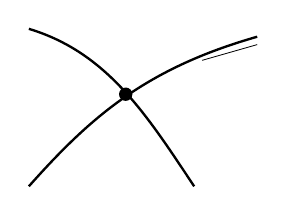
\begin{tikzpicture}[x=1mm, y=1mm]
\draw[line width=.85pt] (0,0) ..controls(8,9)and(15,15)..(29,19);
\draw[line width=.85pt] (0,20) ..controls(10,17)and(15,9)..(21,0);
\draw[line width=.3pt] (22,16)--(29,18);
\fill (12.3,11.7) circle[radius=.85mm];
\end{tikzpicture}}\end{minipage}}}\par\smallskip }
\end{GelfandAdjacentEvidence}


\begin{GelfandAdjacentEvidence}{GELFAND-P000287}{3}
$\mathcal J=($\uwave{Intersect. of primes}$)$.

\Unclear{GELFAND-P000287}{ideal-letter}{The symbol before the equality has a long lower hook: $\mathcal J$ / $\mathcal I$; the letter identity is undetermined.}
\end{GelfandAdjacentEvidence}


We obtain 2 systs. of eqns. $\forall$ solution satisfies \underline{\underline{one}} \underline{\underline{of}} these systems.

\begin{GelfandAdjacentEvidence}{GELFAND-P000287}{4}
(If a geom. point lies on \textbf{[crossed out: ?]} a variety, then it lies on one of the components.)

\Unclear{GELFAND-P000287}{middle-cancelled-word}{A short word or word beginning between “on” and “a variety” is covered by several lines; no reliable sequence of letters is established.}
\end{GelfandAdjacentEvidence}


\begin{GelfandAdjacentEvidence}{GELFAND-P000287}{5}
\textbf{[Cancelled mark in the left margin: ?]}

\Unclear{GELFAND-P000287}{left-cancelled-mark}{A compact repeatedly crossed-out mark with loops. Whether it is a letter, number or nontextual mark is undetermined.}
\end{GelfandAdjacentEvidence}


The rest --- next time.

\begin{GelfandAdjacentEvidence}{GELFAND-P000287}{940}
\underline{\underline{L. Faddeev.}}

\underline{On the results of a computational experiment}, \textbf{[crossed out: ?]} \underline{rel. to Kirillov’s programme}

\hfill\underline{descr. of reprs.}





\Unclear{GELFAND-P000287}{title-cancelled-word}{A word after “experiment,” before “rel.” is cancelled. Its beginning resembles “ре”; the alternatives “реал.” / “рез...” remain unestablished.}
\end{GelfandAdjacentEvidence}


Representation --- quantization of class. mechanics.

Examples and probls. on quantization rules.

\begin{GelfandAdjacentEvidence}{GELFAND-P000287}{7}
$M_{2n}$ --- a sympl. manifold, possess.? $\Omega$ --- a 2-form (nondeg.).\qquad $\Omega=d\omega$.

\Unclear{GELFAND-P000287}{form-abbreviation}{The source abbreviation after “sympl. manifold” is “обл.” / “обал.”; the intermediate stroke is ambiguous. “possess.?” is a provisional abbreviated rendering; the full source word is not established.}
\end{GelfandAdjacentEvidence}


$d\mu=\Omega^n$ --- a measure.

\begin{GelfandAdjacentEvidence}{GELFAND-P000287}{8}
\begin{equation*}f\longrightarrow X_f\qquad (\text{a field from a fn.})\end{equation*}





\SourceFigure{GELFAND-P000287}{hamiltonian-definition-frame}{\par\smallskip\centering{\color{black}\GelfandFitDiagram{\begin{minipage}{68mm}\raggedright \GelfandFitDiagram{\begin{tikzpicture}[baseline=(formula.base)]
\node[inner sep=2pt] (formula) {$\Omega (X_f, Y)=Yf$};
\draw[line width=.85pt] ([xshift=-2mm,yshift=3mm]formula.west)--([xshift=-2mm,yshift=-4mm]formula.south west)--([xshift=2mm,yshift=-4mm]formula.south east)--([xshift=2mm,yshift=3mm]formula.east);
\draw[line width=.5pt] ([xshift=-2mm,yshift=-2.5mm]formula.south west)--([xshift=2mm,yshift=-2.5mm]formula.south east);
\path (formula.south west)++(-2mm,-4mm)coordinate(hatchleft);
\path (formula.south east)++(2mm,-4mm)coordinate(hatchright);
\foreach \k in {0,.05,...,.95}{\draw[line width=.25pt] ($(hatchleft)!\k!(hatchright)$)--++(1.2mm,1.5mm);}
\end{tikzpicture}}\end{minipage}}}\par\smallskip }
\end{GelfandAdjacentEvidence}


Hamiltonian fields $X_f$ form a Lie algebra

\begin{equation*}[X_f, X_g]=X_{\{f, g\}},\end{equation*}

where $\{f, g\}$ --- the Poisson bracket (it is defined by this).

Oper. $X_f$ is antisymm. in $L^2$ with measure $d\mu=\Omega^n$. (It is preserved by Liouville’s theorem.)

To the Lie-algebra elem. $X_f\longrightarrow$ corresponds an oper. in $L^2$.

\underline{1951} Van Hove found a 1-param. family of representations.

\begin{equation*}Z_f=X_f+\alpha\bigl (\omega (X_f)-f\bigr)\end{equation*}



\Needspace{7\baselineskip}
\SourcePage{GELFAND-P000288}{55}
\hfill\GelfandFitDiagram{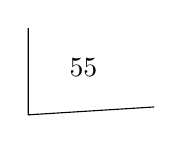
\begin{tikzpicture}[x=1mm, y=1mm]\draw(0,11)--(0,0)--(16,1);\node[inner sep=1pt]at (7,6){$55$};\end{tikzpicture}}

Then the representation condition holds

\begin{equation*}\omega (X_f)-f=\ell_f\end{equation*}

\begin{GelfandAdjacentEvidence}{GELFAND-P000288}{950}
\underline{Van Hove’s assertion:} This is again a repr., not equiv. for any $\alpha$

\begin{equation*}[Z_f, Z_g]=Z_{\{f, g\}}\end{equation*}\end{GelfandAdjacentEvidence}

But this is not yet a passage to quantum mechanics, since everything is still in the space of \underline{all variables}, rather than half of them.

Consider now $SO (3)$ with its nat. repr. in $\mathbb R^3$. On the orbits $(S^2)$ there is a natural compl. structure.

\begin{GelfandAdjacentEvidence}{GELFAND-P000288}{1}
Result of computing $Z_f$, when $X_f$ --- a gener. of the rotation group.





\SourceFigure{GELFAND-P000288}{cancelled-generators}{\par\smallskip\centering{\color{black}\GelfandFitDiagram{\begin{minipage}{68mm}\raggedright \GelfandFitDiagram{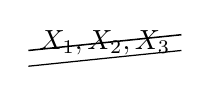
\begin{tikzpicture}[baseline=(cancelled.base)]
\node[inner sep=1pt](cancelled){$X_1, X_2, X_3$};
\draw[line width=.55pt]([xshift=-1mm,yshift=-1mm]cancelled.west)--([xshift=1mm,yshift=1mm]cancelled.east);
\draw[line width=.45pt]([xshift=-1mm,yshift=-3mm]cancelled.west)--([xshift=1mm,yshift=-1mm]cancelled.east);
\end{tikzpicture}}\end{minipage}}}\par\smallskip }
\end{GelfandAdjacentEvidence}


\begin{equation*}x_1^2+x_2^2+x_3^2=a^2\quad\text{--- orbit}\end{equation*}

Functions $x_1, x_2, x_3$. Corresp. Van Hove opers.:

\begin{center}\GelfandFitDiagram{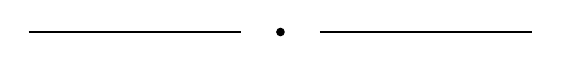
\begin{tikzpicture}[x=1mm, y=1mm]\draw[line width=.6pt](-32,0)--(-5,0);\fill(0,0)circle[radius=.55mm];\draw[line width=.6pt](5,0)--(32,0);\end{tikzpicture}}\end{center}

\begin{GelfandAdjacentEvidence}{GELFAND-P000288}{2}
\underline{\underline{Quantization problem.}}





\SourceFigure{GELFAND-P000288}{phase-plane}{\par\smallskip\centering{\color{black}\GelfandFitDiagram{\begin{minipage}{68mm}\raggedright \GelfandFitDiagram{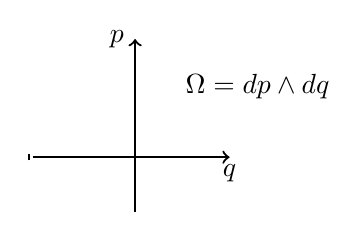
\begin{tikzpicture}[x=1mm, y=1mm]
\draw[->,line width=.8pt](-13,0)--(12,0);
\draw[->,line width=.8pt](0,-7)--(0,15);
\draw[line width=.8pt](-13.5,-.4)--(-13.5,.4);
\node[anchor=north, inner sep=1pt]at (12,-.5){$q$};
\node[anchor=east, inner sep=1pt]at (-1,15){$p$};
\node[anchor=west, inner sep=1pt]at (6,9){$\Omega=dp\wedge dq$};
\end{tikzpicture}}\end{minipage}}}\par\smallskip }
\end{GelfandAdjacentEvidence}


Hamiltonian $f=\dfrac{p^2}{2m}$ (free particle).

An operator must be assigned to it.

\begin{center}\GelfandFitDiagram{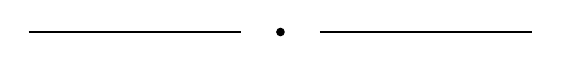
\begin{tikzpicture}[x=1mm, y=1mm]\draw[line width=.6pt](-32,0)--(-5,0);\fill(0,0)circle[radius=.55mm];\draw[line width=.6pt](5,0)--(32,0);\end{tikzpicture}}\end{center}

\begin{GelfandAdjacentEvidence}{GELFAND-P000288}{3}
$f=x_1$.





\Unclear{GELFAND-P000288}{stereographic-diagram}{A rounded contour touches a nearly horizontal line; four sloping strokes extend from its upper region. The rightmost ends above the lower line. A small left hook may be a leftward arrow or a line irregularity; its direction and the exact upper-stroke junctions are undetermined. There are no labels.\par\smallskip\centering{\color{black}\GelfandFitDiagram{\begin{minipage}{68mm}\raggedright \GelfandFitDiagram{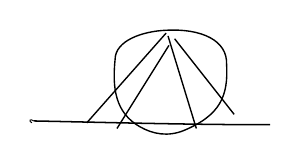
\begin{tikzpicture}[x=.12mm, y=.12mm]
\draw[line width=.5pt](160,126)..controls(135,125)and(106,115)..(106,95)..controls(103,65)and(106,39)..(132,24)..controls(146,16)and(162,13)..(179,20)..controls(217,36)and(226,56)..(224,90)..controls(225,115)and(198,128)..(160,126);
\draw[line width=.55pt](20,30)..controls(75,29)and(178,26)..(270,26);
\draw[line width=.35pt](20,30)..controls(16,33)and(14,30)..(18,28);
\draw[line width=.5pt](160,123)--(76,28);
\draw[line width=.5pt](163,110)--(108,22);
\draw[line width=.5pt](162,120)--(192,22);
\draw[line width=.5pt](169,117)--(232,37);
\end{tikzpicture}}\end{minipage}}}\par\smallskip }
\end{GelfandAdjacentEvidence}


\begin{GelfandAdjacentEvidence}{GELFAND-P000288}{940}
After stereogr. projection (coord. $z$) --- \underline{$\omega$ is not single-valued.}





\begin{equation*}\Omega=a\frac{dz\wedge d\bar z}{(1+|z|^2)^2}\end{equation*}

\begin{equation*}X_i=X_f\quad\text{for }f=x_i\end{equation*}

\begin{equation*}\omega=\frac{a}{i}\frac{1}{1+z\bar z}(z\, d\bar z-\bar z\, dz)\end{equation*}

\Unclear{GELFAND-P000288}{two-form-normalization}{The entry for $\Omega$ has $a$ before the fraction and denominator $(1+|z|^2)^2$. The next entry has factor $a/i$, denominator $1+z\bar z$ and parenthesis $z\, d\bar z-\bar z\, dz$; all these signs are retained.}
\end{GelfandAdjacentEvidence}


No sing. on the plane, but a sing. at $\infty$ (north pole before projection).

\begin{equation*}X_1=\frac{1}{2i}\left ((1-z^2)\frac{\partial}{\partial z}-(1-\bar z^2)\frac{\partial}{\partial\bar z}\right)\end{equation*}

\begin{equation*}Z_1=X_1+\frac{\alpha a}{2}(z+\bar z).\end{equation*}

The analyt. and antianal. parts commute!

Therefore we take

\begin{equation*}Y_1=\frac{1}{2i}(1-z^2)\frac{d}{dz}+\frac{\alpha a}{2}z\end{equation*}

$Y_2, Y_3$ analogously. This is a basis of the Lie alg., satisfying commutation rels.



\Needspace{7\baselineskip}
\SourcePage{GELFAND-P000289}{unlabelled}
They give a repr. of the rotation gr.

\underline{A measure where they are self-adj. exists only for integral $a$!}

\begin{equation*}\frac{1}{(1+\bar z z)^a}\end{equation*}

Square-integrable ones --- a finite number --- polynomials. Therefore a finite-dimensional representation.

\GelfandFitDiagram{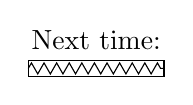
\begin{tikzpicture}[baseline=(word.base)]
\node[inner sep=1pt](word){Next time:};
\draw[line width=.45pt]([yshift=-1mm]word.south west)rectangle([yshift=-3mm]word.south east);
\draw[line width=.4pt,decorate,decoration={zigzag,segment length=1.6mm,amplitude=.7mm}]([yshift=-2mm]word.south west)--([yshift=-2mm]word.south east);
\end{tikzpicture}} Kazhdan;





\begin{GelfandAdjacentEvidence}{GELFAND-P000289}{1}
(Schmid on $L^2$-cohomology (Vezantini, Raghunathan)).

\Unclear{GELFAND-P000289}{announcement-name}{The first surname in parentheses: Vezantini / Vezantin / Vezentini; the crowded final strokes do not establish a definitive reading.}
\end{GelfandAdjacentEvidence}


\underline{Starts at $18^{30}$}. (\underline{end} $20^{30}$)

\begin{GelfandAdjacentEvidence}{GELFAND-P000289}{2}
$6/\mathrm{X}$-69 yr.

\Unclear{GELFAND-P000289}{date-cancelled-sign}{A narrow, densely cancelled mark precedes the date: 1 / 2 / a nontextual mark. Its reading is undetermined.}
\end{GelfandAdjacentEvidence}


\begin{GelfandAdjacentEvidence}{GELFAND-P000289}{3}
\GelfandFitDiagram{
\begin{tikzpicture}[baseline=(name.base)]
\node[inner sep=1pt](name){Dusa mc Duff};
\draw[line width=.6pt](name.south west)--(name.south east);
\draw[line width=.6pt]([xshift=1mm,yshift=3mm]name.north east)--([xshift=1mm,yshift=-3mm]name.south east);
\end{tikzpicture}}

\Unclear{GELFAND-P000289}{speaker-name}{Dusa mc Duff / Дуса mc Duff / Дуза mc Duff. The first name admits mixed or Cyrillic lettering; the written case of “mc” is retained.}
\end{GelfandAdjacentEvidence}


\GelfandFitDiagram{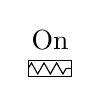
\begin{tikzpicture}[baseline=(word.base)]
\node[inner sep=1pt](word){On};
\draw[line width=.45pt]([yshift=-1mm]word.south west)rectangle([yshift=-3mm]word.south east);
\draw[line width=.4pt,decorate,decoration={zigzag,segment length=1.6mm,amplitude=.7mm}]([yshift=-2mm]word.south west)--([yshift=-2mm]word.south east);
\end{tikzpicture}} \GelfandFitDiagram{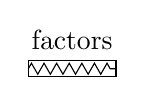
\begin{tikzpicture}[baseline=(word.base)]
\node[inner sep=1pt](word){factors};
\draw[line width=.45pt]([yshift=-1mm]word.south west)rectangle([yshift=-3mm]word.south east);
\draw[line width=.4pt,decorate,decoration={zigzag,segment length=1.6mm,amplitude=.7mm}]([yshift=-2mm]word.south west)--([yshift=-2mm]word.south east);
\end{tikzpicture}} \GelfandFitDiagram{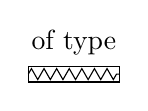
\begin{tikzpicture}[baseline=(word.base)]
\node[inner sep=1pt](word){of type};
\draw[line width=.45pt]([yshift=-1mm]word.south west)rectangle([yshift=-3mm]word.south east);
\draw[line width=.4pt,decorate,decoration={zigzag,segment length=1.6mm,amplitude=.7mm}]([yshift=-2mm]word.south west)--([yshift=-2mm]word.south east);
\end{tikzpicture}} \GelfandFitDiagram{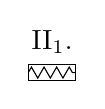
\begin{tikzpicture}[baseline=(word.base)]
\node[inner sep=1pt](word){$\mathrm{II}_1$.};
\draw[line width=.45pt]([yshift=-1mm]word.south west)rectangle([yshift=-3mm]word.south east);
\draw[line width=.4pt,decorate,decoration={zigzag,segment length=1.6mm,amplitude=.7mm}]([yshift=-2mm]word.south west)--([yshift=-2mm]word.south east);
\end{tikzpicture}}

(in English and a woman).





\rotatebox{90}{\GelfandFitDiagram{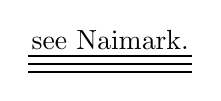
\begin{tikzpicture}[baseline=(reference.base)]
\node[inner sep=1pt](reference){see Naimark.};
\draw[line width=.5pt]([yshift=-.4mm]reference.south west)--([yshift=-.4mm]reference.south east);
\draw[line width=.5pt]([yshift=-1.4mm]reference.south west)--([yshift=-1.4mm]reference.south east);
\draw[line width=.5pt]([yshift=-2.4mm]reference.south west)--([yshift=-2.4mm]reference.south east);
\end{tikzpicture}}}





A subring of the ring of all opers. in Hilb. space is called a factor, if

\begin{GelfandAdjacentEvidence}{GELFAND-P000289}{4}
1) [crossed out: $\forall$?] $X\in M\Longrightarrow X^*\in M$.

\Unclear{GELFAND-P000289}{axiom-cancelled-sign}{After “1)” the sign beneath slanting strokes may be the quantifier $\forall$; it has not been recovered.}
\end{GelfandAdjacentEvidence}


2) $M$ is weakly closed (for $\forall$ seq. $X_n$ the weak limit belongs).

3) The centre consists of opers. proportional to $I$.

\begin{GelfandAdjacentEvidence}{GELFAND-P000289}{5}
\underline{Example.} In the fin.-dimensional case:





\SourceFigure{GELFAND-P000289}{block-matrix}{\par\smallskip\centering{\color{black}\GelfandFitDiagram{\begin{minipage}{68mm}\raggedright \GelfandFitDiagram{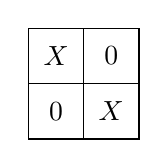
\begin{tikzpicture}[x=7mm, y=7mm]
\draw[line width=.6pt](0,0)rectangle(2,2);
\draw[line width=.6pt](1,0)--(1,2);
\draw[line width=.6pt](0,1)--(2,1);
\node at (.5,1.5){$X$};\node at (1.5,1.5){$0$};
\node at (.5,.5){$0$};\node at (1.5,.5){$X$};
\end{tikzpicture}}\end{minipage}}}\par\smallskip }
\end{GelfandAdjacentEvidence}


Every factor in the fin.-dimensional case is like this: in $H_1\otimes H_2$ consider opers. $X\otimes1$ ($X$ --- arbitrary).

A vect. --- a matrix $\xi_{ik}$. An oper. --- acts on the 1st coordinate.

\begin{center}\GelfandFitDiagram{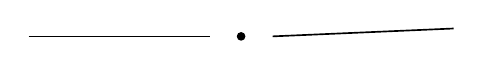
\begin{tikzpicture}[x=1mm, y=1mm]\draw[line width=.6pt](-27,0)--(-4,0);\fill(0,0)circle[radius=.55mm];\draw[line width=.6pt](4,0)--(27,1);\end{tikzpicture}}\end{center}

Every weakly closed ring (with involution) decomposes into a direct integral of factors.

Von Neumann \GelfandFitDiagram{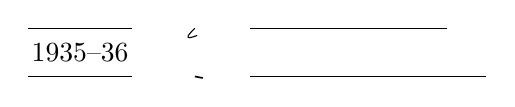
\begin{tikzpicture}[baseline=(years.base), x=1mm, y=1mm]
\node[inner sep=1pt](years)at (0,0){1935--36};
\draw[line width=.5pt]([yshift=1.5mm]years.north west)--([yshift=1.5mm]years.north east);
\draw[line width=.5pt]([yshift=-1.5mm]years.south west)--([yshift=-1.5mm]years.south east);
\draw[line width=.5pt]([xshift=15mm,yshift=1.5mm]years.north east)--([xshift=40mm,yshift=1.5mm]years.north east);
\draw[line width=.5pt]([xshift=15mm,yshift=-1.5mm]years.south east)--([xshift=45mm,yshift=-1.5mm]years.south east);
\draw[line width=.4pt]([xshift=8mm,yshift=1.5mm]years.north east)..controls([xshift=6.6mm,yshift=.2mm]years.north east)and([xshift=7mm,yshift=.1mm]years.north east)..([xshift=8.3mm,yshift=.6mm]years.north east);
\draw[line width=.6pt]([xshift=8mm,yshift=-1.5mm]years.south east)--([xshift=9mm,yshift=-1.7mm]years.south east);
\end{tikzpicture}}





Let $M$ --- a factor; then $\dfrac{X+X^*}{2}$, $\dfrac{X-X^*}{2i}$ generate them.

(self-adj.) $a=\int\lambda\, de_\lambda$, $e_\lambda\in$ the factor, and generate the factor.

A factor is generated by projections with $e^2=e$, $e^*=e$.



\Needspace{7\baselineskip}
\SourcePage{GELFAND-P000290}{56}
\hfill\GelfandFitDiagram{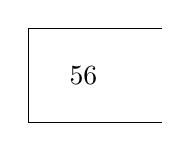
\begin{tikzpicture}[x=1mm, y=1mm]\draw(17,12)--(0,12)--(0,0)--(17,0);\node at (7,6){$56$};\end{tikzpicture}}

\begin{GelfandAdjacentEvidence}{GELFAND-P000290}{1}
If [crossed out: illegible] there exists an \GelfandFitDiagram{\begin{tikzpicture}[baseline=(isometry.base)]
\node[inner sep=1pt](isometry){isometry};
\node[draw, line width=.5pt, rounded corners=4pt, inner sep=1pt, anchor=south](partial)at ([yshift=3mm]isometry.north){partial};
\draw[line width=.5pt](partial.south)--([yshift=.5mm]isometry.north);
\end{tikzpicture}} from $M$, joining the subsp. corresponding to the projections, then the 2 \GelfandFitDiagram{\begin{tikzpicture}[baseline=(operators.base)]
\node[inner sep=1pt](operators){opers.};
\node[anchor=north, inner sep=1pt]at ([yshift=-.7mm]operators.south){(subsp.)};
\end{tikzpicture}} are called equivalent.

\Unclear{GELFAND-P000290}{top-cancellation}{After “If” and before “there exists”, tall signs are densely crossed by diagonals; the underlying signs have not been separated or read.}
\end{GelfandAdjacentEvidence}










If equiv. ones are identified, then \underline{an ordering results} (by inclusion).

Equiv. classes of projection opers. can be added.

Hence subsp. can be measured (assign numbers to a subsp.).

(No Archim. axiom --- $\infty$ is present).

\underline{\underline{Thm.}} If there is a $\min$ subsp., then it is isom. to the ring of all opers. in Hilb. space.

\begin{equation*}R=M\otimes M'\qquad (M'\text{ --- commutant factor}).\end{equation*}

No $\min\Longrightarrow$ either $\mathrm{II}_1$, $\mathrm{II}_\infty$ or $\mathrm{III}$.

\begin{GelfandAdjacentEvidence}{GELFAND-P000290}{2}
$\mathrm{II}_1$ --- there is never a $\min$, but everything is meas. by numbers in $(0,1]$ (there is a $\max$) and the Archim. axiom.









\SourceFigure{GELFAND-P000290}{type-II1-heading}{\par\smallskip\centering{\color{black}\GelfandFitDiagram{\begin{minipage}{68mm}\raggedright \GelfandFitDiagram{\begin{tikzpicture}[baseline=(heading.base), x=1mm, y=1mm]
\node[inner sep=1pt](heading)at (5,4){$\mathrm{II}_1$.};
\draw[line width=.6pt](0,0)--(11,.5);
\draw[line width=.6pt](0,-3)--(11,-2.5);
\draw[line width=.4pt](1,-2.9)--(1,-.1);
\draw[line width=.4pt](3,-2.8)--(3,.1);
\draw[line width=.4pt](5,-2.7)--(5,.2);
\draw[line width=.4pt](7.5,-2.6)..controls(6,-1.1)and(7,0)..(8,.3);
\draw[line width=.4pt](8.2,.3)..controls(8.2,-1.6)and(8.8,-1.5)..(9,-.3);
\end{tikzpicture}}\end{minipage}}}\par\smallskip }
\end{GelfandAdjacentEvidence}


\begin{GelfandAdjacentEvidence}{GELFAND-P000290}{3}
[cancelled sign: $\forall$?] $\forall$ oper. has a trace and $\det$; the \underline{minimax} theory of eigenvalues holds (everything that holds for matrices).

\Unclear{GELFAND-P000290}{trace-cancelled-sign}{Before the legible $\forall$, a small sign with two slanting strokes and a crossbar is cancelled. Its possible reading as $\forall$ is not established.}
\end{GelfandAdjacentEvidence}


\begin{equation*}\operatorname{Tr}(a)=\int\lambda\, d (\dim e_\lambda)\qquad (\dim\text{ from }0\text{ to }1)\end{equation*}

The space itself has not yet been discovered.

Which factors of type $\mathrm{II}_1$?

1) hyperfinite Murray and Neumann --- there is only one

2) J. Shvarts

3) Ching

4) Sakai

5--6) Dixmier, Lance

7--8) Zeller-Meier

\begin{GelfandAdjacentEvidence}{GELFAND-P000290}{4}
$7,8'$) Stepin, Golodets









\SourceFigure{GELFAND-P000290}{continuum-separator}{\par\smallskip\centering{\color{black}\GelfandFitDiagram{\begin{minipage}{68mm}\raggedright \GelfandFitDiagram{\begin{tikzpicture}[x=1mm, y=1mm]
\node[anchor=east, inner sep=1pt]at (-2,0){\shortstack{Continuum of\\factors}};
\draw[line width=.6pt](0,-6)--(1,6);
\draw[line width=.6pt](1.7,-6)--(2.7,6);
\node[anchor=west, inner sep=1pt]at (5,1){Dusa Mc Duff};
\end{tikzpicture}}\end{minipage}}}\par\smallskip }
\end{GelfandAdjacentEvidence}




\Needspace{7\baselineskip}
\SourcePage{GELFAND-P000291}{unlabelled}
\underline{$13/\mathrm{X}$-69 yr.}\hfill\underline{Next time Minlos and Sinai.}

\underline{Gelfand.}

\GelfandFitDiagram{\begin{tikzpicture}[baseline=(work.base)]
\node[inner sep=1pt](work){On Araki’s work.};
\draw[line width=.55pt,decorate,decoration={snake,amplitude=.5mm,segment length=2.5mm}]([yshift=-1mm]work.south west)--([yshift=-1mm]work.south east);
\end{tikzpicture}}





\underline{\underline{Question:}} Let

\begin{equation*}
\begin{pmatrix}\alpha (t)&\beta (t)\\-\bar\beta (t)&\overline{\alpha (t)}\end{pmatrix}=u (t)
\end{equation*}

a unit. matrix with $\det1$,

\begin{equation*}|\alpha (t)|^2+|\beta (t)|^2=1,\qquad t\in[0,1].\end{equation*}

Find all irred. unit. representations of this group. This has not been done.

$\operatorname{supp}$ of repr. $F$ --- the smallest closed set for which the condition holds

\begin{equation*}u (t)\equiv1\quad\forall t\in U (F)\Longrightarrow T_{u (t)}=I\end{equation*}

\underline{Problem:} does an irred. unit. representation exist with $\operatorname{supp}$ --- an interval.

\begin{center}\GelfandFitDiagram{\begin{tikzpicture}[x=1mm, y=1mm]\draw[line width=.55pt](-18,0)--(-4,0);\fill(0,0)circle[radius=.35mm];\draw[line width=.55pt](4,0)--(18,0);\end{tikzpicture}}\end{center}

$\operatorname{supp}$ --- a point --- the operator $u (t_0)$ (2-dim. repr.).

This is the repr. $\delta (t-t_0)$.

\begin{GelfandAdjacentEvidence}{GELFAND-P000291}{1}
\begin{equation*}e:\ u (t)\longrightarrow T^e_{u (t_0)}\qquad\delta_e (t-t_0)\end{equation*}

\Unclear{GELFAND-P000291}{representation-index}{Before the colon, above $T$ and below $\delta$ is a looped sign: $e$ / $\ell$. The typeset line shows the visual candidate $e$; the letter is undetermined.}
\end{GelfandAdjacentEvidence}


\begin{equation*}u (t)\longrightarrow u (t_1)\otimes u (t_2)\end{equation*}

an irred. repr. with $\operatorname{supp}$ --- a pair of points.

\begin{GelfandAdjacentEvidence}{GELFAND-P000291}{2}
(a repr., in effect, of a direct sum of 2 [crossed out: matr.?] groups of matrices).

\Unclear{GELFAND-P000291}{right-cancelled-word}{The parenthetical insertion is on the right. After “2”, a short word is cancelled, possibly “matr.”; below it is the separate entry “groups of matrices”. The cancelled word’s reading is undetermined.}
\end{GelfandAdjacentEvidence}


One can take $n$ points.

For a countable set this can no longer be done (it can be done for a convergent seq.).

\GelfandFitDiagram{\begin{tikzpicture}[baseline=(araki.base)]
\node[inner sep=1pt](araki){Araki.};
\draw[line width=.55pt]([yshift=-.8mm]araki.south west)rectangle([yshift=-2.8mm]araki.south east);
\draw[line width=.45pt,decorate,decoration={zigzag,segment length=1.8mm,amplitude=.7mm}]([yshift=-1.8mm]araki.south west)--([yshift=-1.8mm]araki.south east);
\end{tikzpicture}}





Idea:

\begin{equation*}e^K=\bigoplus_{n=0}^{\infty}S^n (K)\end{equation*}

($K$ --- Hilb. space)

\begin{GelfandAdjacentEvidence}{GELFAND-P000291}{3}
\begin{equation*}e^{\varphi}=\bigoplus_{n=0}^{\infty}\frac{1}{\sqrt{n!}}\varphi\otimes\varphi\otimes\cdots\otimes p\end{equation*}

\Unclear{GELFAND-P000291}{coherent-last-symbol}{The last factor after $\otimes$ has a descending stroke and an upper-right loop: $p$ / $\rho$; its possible identification with the preceding $\varphi$ signs is not established. The formula shows the visual candidate $p$.}
\end{GelfandAdjacentEvidence}


$\sqrt{n!}$, so that $(e^{\varphi}, e^{\psi})=e^{(\varphi,\psi)}$.

$K\to e^K$ --- a functorial passage

\begin{equation*}K_1\oplus K_2\longrightarrow e^{K_1}\otimes e^{K_2}\end{equation*}

At $\forall$ point $t$ we specify a representation in the space $K (t)$ (e.g. 2-dimensional)

\begin{equation*}\int_0^1 K (t)\, dt\end{equation*}



\Needspace{7\baselineskip}
\SourcePage{GELFAND-P000292}{57}
\hfill\GelfandFitDiagram{\begin{tikzpicture}[x=1mm, y=1mm]\draw(0,13)--(0,0)--(17,1);\node at (7,6){$57$};\end{tikzpicture}}

Consider $e^{\int_0^1 K (t)\, dt}$.

A repr. is obtained in it (from funct.) which is reducible.

\begin{center}\GelfandFitDiagram{\begin{tikzpicture}[x=1mm, y=1mm]\draw[line width=.55pt](-20,0)--(-3,0);\fill(0,0)circle[radius=.4mm];\draw[line width=.55pt](3,0)--(20,.4);\end{tikzpicture}}\end{center}

The gr. of matrices of order 1 $\alpha (t)=e^{x (t)}$.

\begin{GelfandAdjacentEvidence}{GELFAND-P000292}{1}
“Nepr.” repr.

\Unclear{GELFAND-P000292}{representation-abbreviation}{The source abbreviation “Непр.” before “repr.” is retained as “Nepr.” without expansion; continuous/irreducible has not been selected from context.}
\end{GelfandAdjacentEvidence}


\begin{gather*}e^{x (t)}\longrightarrow C,\qquad e^{x_1(t)}e^{x_2(t)}\longrightarrow C_1C_2,\qquad C=e^a\\x (t)\longrightarrow a\end{gather*}

\begin{GelfandAdjacentEvidence}{GELFAND-P000292}{2}
$a$ --- a lin. funct. of $X (t)$ --- a generalized func. or distribution.

\Unclear{GELFAND-P000292}{argument-case}{In the line about the linear functional, the letter $X (t)$ / $x (t)$ is larger than the nearby $x$ signs; its case is undetermined. The candidate $X (t)$ is shown.}
\end{GelfandAdjacentEvidence}


\begin{equation*}\delta (t-t_0):\qquad e^{x (t)}\longrightarrow e^{x (t_0)}\end{equation*}

\begin{equation*}x (t)\longrightarrow e^{\int_0^1 a (t)x (t)\, dt}\end{equation*}

On the circle an integrality condition is added.

\begin{center}\GelfandFitDiagram{\begin{tikzpicture}[x=1mm, y=1mm]\draw[line width=.55pt](-11,0)--(-3,0);\fill(0,0)circle[radius=.4mm];\draw[line width=.55pt](3,0)--(11,.4);\end{tikzpicture}}\end{center}

A repr. here is a generalization of a distribution.



\Needspace{7\baselineskip}
\SourcePage{GELFAND-P000293}{60}
\hfill\GelfandFitDiagram{\begin{tikzpicture}[x=1mm, y=1mm]\draw(0,13)--(0,0)--(17,1);\node at (7,6){$60$};\end{tikzpicture}}

\uwave{17/XI-69 yr.}\qquad\underline{Hewitt.}

\uwave{One result} (sharp for all \underline{comp.} groups)

as for the circle.





\begin{GelfandAdjacentEvidence}{GELFAND-P000293}{1}
[crossed out: illegible]

\Unclear{GELFAND-P000293}{upper-cancelled-sign}{Dense crossing strokes precede the heading “On s-numbers”; the underlying letters or signs have not been read.}
\end{GelfandAdjacentEvidence}


\underline{On $s$-numbers:}

\begin{flushright}\begin{minipage}{.76\linewidth}
\underline{Gantmakher;}\par
\underline{Wielandt}\par
\underline{Berezin, Gelfand}\qquad Trudy \underline{M. M. O.} ---\par
--- \underline{$\forall$ semisimple Lie groups.}\par
from repr. theory for a compl. func.
\end{minipage}\end{flushright}





\underline{H. Weyl}\qquad\underline{and}\qquad\underline{Ky Fan.}

\begin{GelfandAdjacentEvidence}{GELFAND-P000293}{2}
[crossed out: illegible] All this is for an arbitrary group and a class of representations:

\Unclear{GELFAND-P000293}{middle-cancelled-sign}{Before “All this”, joined vertical and slanting strokes are cancelled; the underlying sequence is undetermined.}
\end{GelfandAdjacentEvidence}


\begin{GelfandAdjacentEvidence}{GELFAND-P000293}{3}
\begin{equation*}\|\hat f\|_p=(\sum_{\sigma\in\Sigma}d_\sigma\|\hat f (\sigma\|_p^p)\end{equation*}

\Unclear{GELFAND-P000293}{p-norm-formula}{After $\sigma$ in the argument are two vertical strokes without a separate closing round parenthesis. No exponent is read after the large right parenthesis. The $\sigma$ next to $d$ may be a subscript or on the line; the candidate $d_\sigma$ is shown.}
\end{GelfandAdjacentEvidence}


\underline{Peter--Weyl--Plancherel thm.}

\begin{equation*}\|\hat f\|_2^2=\int_G|f|^2\, d\lambda;\end{equation*}

\begin{GelfandAdjacentEvidence}{GELFAND-P000293}{4}
\begin{equation*}\|\hat f\|_\infty=\sup\{\|\hat f (\sigma)\|_{\mathfrak{S}_\infty}:\ \sigma\in\Sigma\}.\end{equation*}

\Unclear{GELFAND-P000293}{infinity-norm-subscript}{Before $\infty$ is an S-shaped sign with a long crossing stroke: $\mathfrak{S}_\infty$ / $S_\infty$. This line shows the blackletter candidate; the following lemma retains ordinary $S$.}
\end{GelfandAdjacentEvidence}


\underline{Riem.--Lebesgue lemma:}

\begin{equation*}\forall f\in L_1(G),\quad\forall\varepsilon>0\quad\{\sigma:\ \|\hat f (\sigma)\|_{S_\infty}>\varepsilon\}\end{equation*}

--- a finite set.

\underline{\underline{Kunze’s thm.}}\qquad $1<p<2$

\begin{equation*}\|\hat f\|_{p\prime}\le\|f\|_p.\end{equation*}

\begin{GelfandAdjacentEvidence}{GELFAND-P000293}{5}
(Hausd.--Yun.).

\Unclear{GELFAND-P000293}{young-abbreviation}{After “Hausd.-”, the abbreviation is Yun. / Yung.; the final hooked stroke before the full stop is not established as part of н or a separate г.}
\end{GelfandAdjacentEvidence}


\underline{Thm.} of Hardy--Littlewood --- equality only for \GelfandFitDiagram{\begin{tikzpicture}[baseline=(equality.base)]
\node[inner sep=1pt](equality){$f (x)=\alpha e^{inx}; $};
\draw[line width=.55pt]([yshift=1mm]equality.south west)--([yshift=-1mm]equality.south west)--([yshift=-1mm]equality.south east)--([yshift=1mm]equality.south east);
\end{tikzpicture}}





For a general group things are not so simple: there, for funcs. of the form

$\chi$ --- a cont. func. on an open subgroup $G_0$,\quad $\chi (e)=1$,\quad $\chi (xy)=\chi (x)\chi (y)$,

$\chi=0$ outside $G_0$.

There are analogues of the Riesz--Thorin theorems.



\Needspace{7\baselineskip}
\SourcePage{GELFAND-P000294}{unlabelled}
\GelfandFitDiagram{\begin{tikzpicture}[baseline=(date.base)]
\node[inner sep=1pt](date){23.2.70 yr.};
\draw[line width=.6pt]([yshift=-.8mm]date.south west)rectangle([yshift=-2.5mm]date.south east);
\draw[line width=.5pt,decorate,decoration={zigzag,segment length=2mm,amplitude=.6mm}]([yshift=-1.65mm]date.south west)--([yshift=-1.65mm]date.south east);
\end{tikzpicture}}





\begin{GelfandAdjacentEvidence}{GELFAND-P000294}{1}
\underline{\underline{Kazhdan}} \underline{\underline{on}} \underline{\underline{Griffiths’s}} \underline{\underline{work.}}





\Unclear{GELFAND-P000294}{upper-left-sketch}{On the left is an oval contour with an interior point and six long curves above it. A small loop and nearly parallel lower strokes occur at the left edge. The short-stroke connections and curve continuations are undetermined; there are no labels or definite arrows.\par\smallskip\centering{\color{black}\GelfandFitDiagram{\begin{minipage}{68mm}\raggedright \GelfandFitDiagram{\begin{tikzpicture}[x=.2mm, y=.2mm]
\draw[line width=.55pt](28,60)..controls(0,34)and(17,6)..(64,5)..controls(99,-1)and(158,20)..(152,58)..controls(153,87)and(115,92)..(85,88)..controls(61,89)and(39,76)..(28,60);
\fill(83,50)circle[radius=2.4];
\draw[line width=.5pt](21,203)..controls(9,167)and(0,80)..(22,52);
\draw[line width=.5pt](47,198)..controls(35,169)and(22,84)..(30,61)..controls(34,54)and(36,51)..(45,52);
\draw[line width=.5pt](73,198)..controls(58,171)and(48,59)..(68,18);
\draw[line width=.5pt](85,174)..controls(87,145)and(81,90)..(87,85)..controls(89,72)and(95,65)..(101,63);
\draw[line width=.5pt](110,172)..controls(104,144)and(98,68)..(106,48)..controls(111,43)and(115,38)..(121,37);
\draw[line width=.5pt](129,161)..controls(130,135)and(126,65)..(128,42);
\draw[line width=.5pt](40,57)..controls(42,45)and(49,25)..(55,16);
\draw[line width=.45pt](21,58)..controls(17,50)and(28,44)..(36,53);
\end{tikzpicture}}\end{minipage}}}\par\smallskip }
\end{GelfandAdjacentEvidence}


\begin{equation*}T:\ H^i (V_s)\longrightarrow H^i (V_s)\end{equation*}

(on going around a puncture)

\begin{equation*}\exists N,\ \text{such that}\quad (T^N-1)^{i+1}=0\end{equation*}

\begin{GelfandAdjacentEvidence}{GELFAND-P000294}{2}
($T$ is unipotent).

\Unclear{GELFAND-P000294}{monodromy-qualification}{The formula is followed by the separate entry “($T$ is unipotent)”, with no $N$ on $T$ and no “quasi” prefix; the entry is retained.}
\end{GelfandAdjacentEvidence}


\begin{GelfandAdjacentEvidence}{GELFAND-P000294}{3}
\begin{center}\GelfandFitDiagram{\begin{tikzpicture}[x=1mm, y=1mm]\draw[line width=.55pt](-30,0)--(-4,0);\fill(0,0)circle[radius=.35mm];\draw[line width=.55pt](4,0)--(30,0);\end{tikzpicture}}\end{center}





\SourceFigure{GELFAND-P000294}{bundle-W}{\par\smallskip\centering{\color{black}\GelfandFitDiagram{\begin{minipage}{68mm}\raggedright \GelfandFitDiagram{\begin{tikzpicture}[x=1mm, y=1mm]\node at (0,15){$W$};\draw[->,line width=.65pt](0,11)--(0,3);\node at (0,0){$S$};\end{tikzpicture}}\end{minipage}}}\par\smallskip }
\end{GelfandAdjacentEvidence}


an algebraic bundle

base --- a 1-dim. alg. variety (a Riem. surface with punctures).

\begin{equation*}\pi_1(S):\ H^K (V_s)\longrightarrow H^K (V_s)\qquad (\text{coeffs. }C).\end{equation*}

\begin{GelfandAdjacentEvidence}{GELFAND-P000294}{4}
\uwave{and defines a vect. bundle} [crossed out: an illegible sign] (analytic)

\Unclear{GELFAND-P000294}{cancelled-bundle-sign}{A narrow cancelled sign occurs between “bundle” and “(analytic)”; the underlying letter is undetermined.}
\end{GelfandAdjacentEvidence}
\begin{GelfandAdjacentEvidence}{GELFAND-P000294}{5}






\SourceFigure{GELFAND-P000294}{bundle-E}{\par\smallskip\centering{\color{black}\GelfandFitDiagram{\begin{minipage}{68mm}\raggedright \GelfandFitDiagram{\begin{tikzpicture}[x=1mm, y=1mm]\node at (0,15){$E$};\draw[->,line width=.65pt](0,11)--(0,3);\node at (0,0){$S$};\end{tikzpicture}}\end{minipage}}}\par\smallskip }
\end{GelfandAdjacentEvidence}


$O (E)$ --- the sheaf of germs of analyt. sects.

There is a canon. connection from parallel transports on the universal cover $\tilde S$. (There it is a direct product.)

We shall study it near a puncture.

Write the connection in the form of an eqn.

\begin{equation*}\begin{array}{l}f_1(z)\text{ --- sections}\\\ldots\\f_n (z)\end{array}\qquad (\text{a basis near }z).\end{equation*}

\begin{GelfandAdjacentEvidence}{GELFAND-P000294}{6}
Picard--Fuchs eqn. $\dfrac{\partial}{\partial z}=A (z)$

\Unclear{GELFAND-P000294}{connection-operator}{This line literally reads $\partial/\partial z=A (z)$, with no $f (z)$ on either side. A separate equation with $f (z)$ occurs below; both entries are retained.}
\end{GelfandAdjacentEvidence}


\begin{GelfandAdjacentEvidence}{GELFAND-P000294}{7}
Transport $f_1(z)$ horizontally to $z+\delta z$ and expand in the basis [crossed out: $z+\delta z$, followed by illegible signs] $f_1(z+\delta z),\ldots$

\Unclear{GELFAND-P000294}{cancelled-basis-formula}{After “basis”, the cancelled sequence $z+\delta z$ has an illegible ending; there may be another $z$ on the right. The uncancelled $f_1(z+\delta z),\ldots$ is read separately.}
\end{GelfandAdjacentEvidence}


Consider any flat sect. of the bundle. it satisfies the eqn.

\begin{equation*}\frac{\partial}{\partial z}f (z)=A (z)f (z)\end{equation*}

and all flat sects. are solutions of this eqn.

\begin{GelfandAdjacentEvidence}{GELFAND-P000294}{940}
\underline{\underline{Example of flat sections.}}

Let $\Phi_z$ --- a cycle in the fibre ($K$-dimensional).

\Unclear{GELFAND-P000294}{overwritten-cycle}{After “Let”, a large heavily retraced letter reads $\Phi_z$ / $\phi_z$; its original form and whether it was retraced or corrected are undetermined. The candidate $\Phi_z$ is shown.}
\end{GelfandAdjacentEvidence}


\begin{equation*}\Phi_z\subset V_z,\qquad\Phi_{z'}\subset V_{z'}.\end{equation*}



\Needspace{7\baselineskip}
\SourcePage{GELFAND-P000295}{62}
\hfill\GelfandFitDiagram{\begin{tikzpicture}[x=1mm, y=1mm]\draw(0,13)--(0,0)--(17,1);\node at (7,6){$62$};\end{tikzpicture}}





\begin{GelfandAdjacentEvidence}{GELFAND-P000295}{1}
--- an example of a flat section. ---

\Unclear{GELFAND-P000295}{pairing-index}{The first entry has two pairs of round parentheses; the outer ones extend downward toward the explanation. The retraced sign after $f$ admits $f_i (z)$ / $f^i (z)$. Subscript $i$ is shown; the parentheses’ relation to the explanation below is undetermined.\par\smallskip\centering{\color{black}\GelfandFitDiagram{\begin{minipage}{68mm}\raggedright \GelfandFitDiagram{\begin{tikzpicture}[x=1mm, y=1mm]
\node[inner sep=1pt]at (0,6){$(f_i (z),\phi_z)$};
\node[inner sep=1pt]at (2,-3){value of cohom. on hom.};
\draw[line width=.55pt](-23,14)..controls(-28,9)and(-28,-5)..(-22,-7);
\draw[line width=.55pt](23,14)..controls(26,8)and(26,-2)..(23,-4);
\end{tikzpicture}}\end{minipage}}}\par\smallskip }
\end{GelfandAdjacentEvidence}


\hfill --- a vector func.





\underline{\underline{Thm.}} (Griffiths)

$\exists$ a basis $f_i (z)$, such that the eqn. has a reg. singular point,

i.e. $zA (z)$ extends holomorphically to $0$. (regular).

(Allows one to infer the behaviour of periods on approaching a singular point).

\begin{GelfandAdjacentEvidence}{GELFAND-P000295}{950}
\underline{Corollary}

Consider any flat section --- a sol. of the eqn. Then it expands in a series

\begin{equation*}\sum_{n\le0}z^{n/N}\big (\underline{C_{n0}}+\underline{C_{n1}}\ln z+\ldots+\underline{c_{nk}}\ln^k z\big)\end{equation*}

\Unclear{GELFAND-P000295}{series-indices}{The index $n$ / $\nu$ is heavily retraced. The bound sign resembles $\le$; $n\le0$ is shown, with no established upper limit. The last initial letter is smaller than the earlier $C$ signs and c-/e-shaped; its case and reading are undetermined, with candidate $c_{nk}$ shown. Three coefficients are underlined.}
\end{GelfandAdjacentEvidence}


\begin{GelfandAdjacentEvidence}{GELFAND-P000295}{940}
\underline{\underline{Lemma}}\qquad $\forall$ flat sect. $\phi_z$

\begin{equation*}|\Phi_z|\le C|z|^{-a}|\ln z|^b\end{equation*}

\Unclear{GELFAND-P000295}{bound-exponent}{The exponent on $|\ln z|$ has two crowded loops: $b$ / $\beta$. The candidate $b$ is shown. The bound has a large $\Phi$, while the preceding line has a lighter $\phi$; the distinction is retained.}
\end{GelfandAdjacentEvidence}
\begin{GelfandAdjacentEvidence}{GELFAND-P000295}{4}






\SourceFigure{GELFAND-P000295}{lower-dotted-rule}{\par\smallskip\centering{\color{black}\GelfandFitDiagram{\begin{minipage}{68mm}\raggedright $\cdot\quad\cdot\quad\cdot\quad\cdot\quad\cdot\quad\cdot\quad\cdot\quad\cdot\quad\cdot\quad\cdot\quad\cdot\quad\cdot$\end{minipage}}}\par\smallskip }
\end{GelfandAdjacentEvidence}




\Needspace{7\baselineskip}
\SourcePage{GELFAND-P000296}{unlabelled}
7/IX-1970 yr.\qquad\GelfandFitDiagram{\begin{tikzpicture}[baseline=(word.base)]
\node[inner sep=1pt](word){Seminar};
\draw[line width=.55pt]([yshift=-.8mm]word.south west)rectangle([yshift=-2.5mm]word.south east);
\draw[line width=.45pt,decorate,decoration={zigzag,segment length=2mm,amplitude=.6mm}]([yshift=-1.65mm]word.south west)--([yshift=-1.65mm]word.south east);
\end{tikzpicture}} \GelfandFitDiagram{\begin{tikzpicture}[baseline=(word.base)]
\node[inner sep=1pt](word){of Gelfand.};
\draw[line width=.55pt]([yshift=-.8mm]word.south west)rectangle([yshift=-2.5mm]word.south east);
\draw[line width=.45pt,decorate,decoration={zigzag,segment length=2mm,amplitude=.6mm}]([yshift=-1.65mm]word.south west)--([yshift=-1.65mm]word.south east);
\end{tikzpicture}}





\underline{Seminar programme.}

1. Kazhdan on the relation between formal and algebraic geometry.

2. Arnold: Griffiths’s works.

3. Mityagin and Henkin on their works.

\begin{GelfandAdjacentEvidence}{GELFAND-P000296}{1}
[cancelled number: 4.?] $1^{\prime}$. Moishezon on Artin’s works.

\Unclear{GELFAND-P000296}{cancelled-programme-number}{Before the separate uncancelled $1^{\prime}$, a number or sign is densely cancelled, possibly 4.; the number has not been recovered.}
\end{GelfandAdjacentEvidence}


?. $K$-theory of finite groups

\hfill Brown, Tate, Tomson, Swan, Katz.

(Kazhdan, Bernstein, etc.)

4. Hironaka.

\begin{GelfandAdjacentEvidence}{GELFAND-P000296}{950}
\underline{For next semester.}

$\zeta$-func.\qquad ($p$-adic harm. analysis).

Finite groups.\end{GelfandAdjacentEvidence}

\begin{center}\GelfandFitDiagram{\begin{tikzpicture}[x=1mm, y=1mm]\draw[line width=.55pt](-30,0)--(-4,0);\fill(0,0)circle[radius=.5mm];\draw[line width=.55pt](4,0)--(30,0);\end{tikzpicture}}\end{center}

\underline{\underline{Kazhdan.}}

Where is this expounded?





\begin{GelfandAdjacentEvidence}{GELFAND-P000296}{2}
part \underline{III}, $N=1$.

\SourceFigure{GELFAND-P000296}{cohomology-bracket}{\par\smallskip\centering{\color{black}\GelfandFitDiagram{\begin{minipage}{68mm}\raggedright \GelfandFitDiagram{\begin{tikzpicture}
\node[inner sep=2pt](refs){\begin{minipage}{.78\linewidth}1. Serre, “Coherent alg. sheaves”.\par\smallskip
2. More modern, but less pleasant\qquad Dieudonné\qquad Mat. 9:1\par\smallskip
3. Lectures of Yu. I. Manin (part 1)\qquad Alg. geometry.\par\smallskip
4. 3rd volume of Grothendieck\qquad I. H. E. S., vol. 12\end{minipage}};
\draw[line width=.55pt]([xshift=1mm,yshift=-1mm]refs.north west)--([xshift=-2mm,yshift=-1mm]refs.north west)--([xshift=-2mm,yshift=1mm]refs.south west)--([xshift=1mm,yshift=1mm]refs.south west);
\node[rotate=90, anchor=south, inner sep=1pt]at ([xshift=-4mm]refs.west){\shortstack{Cohomology of\\aff. and proj. schemes.}};
\end{tikzpicture}}\end{minipage}}}\par\smallskip }
\end{GelfandAdjacentEvidence}


\underline{Gelfand’s remark:} learn Serre’s books “Finite groups” and “Lie gr. and Lie alg.”.

\begin{GelfandAdjacentEvidence}{GELFAND-P000296}{3}
(Part of the minimum in lin. algebra)





\SourceFigure{GELFAND-P000296}{parts-arrow}{\par\smallskip\centering{\color{black}\GelfandFitDiagram{\begin{minipage}{68mm}\raggedright \GelfandFitDiagram{\begin{tikzpicture}[x=1mm, y=1mm]
\draw[->,line width=.6pt](0,9)--(2,1);
\node[anchor=north west, inner sep=1pt]at (0,0){1 and 2nd part.};
\end{tikzpicture}}\end{minipage}}}\par\smallskip }
\end{GelfandAdjacentEvidence}


\underline{Part 1:}\qquad\GelfandFitDiagram{\begin{tikzpicture}[baseline=(part.base)]\node[inner sep=1pt](part){Cohomology of coherent sheaves.};\draw[dashed,line width=.45pt]([yshift=-1mm]part.south west)--([yshift=-1mm]part.south east);\end{tikzpicture}}





\S1. \underline{Definition of a scheme.}

A scheme --- a ringed space of a special kind

\GelfandFitDiagram{\begin{tikzpicture}[baseline=(space.base)]
\node[inner sep=1pt](space){Top. space,};
\draw[line width=.5pt](space.south west)--([yshift=-1mm]space.south west)--([yshift=-1mm,xshift=5mm]space.south west)--([yshift=-5mm,xshift=5mm]space.south west)--([yshift=-5mm,xshift=-5mm]space.south east)--([yshift=-1mm,xshift=-5mm]space.south east)--([yshift=-1mm]space.south east);
\node[inner sep=1pt]at ([yshift=-3mm]space.south){$X$};
\end{tikzpicture}} equipped with a sheaf of rings. $O$\qquad (structure sheaf).





Affine scheme.\qquad $A$ --- a comm. ring with 1.

\begin{GelfandAdjacentEvidence}{GELFAND-P000296}{4}
$\operatorname{Spec}A$\qquad Points --- prime ideals $\wp\subset A$.

\Unclear{GELFAND-P000296}{prime-ideal-symbol}{The looped ideal sign admits $\wp$ / $\mathfrak p$ / $p$. Both occurrences show the nearest available glyph $\wp$; the letter’s identity is undetermined.}
\end{GelfandAdjacentEvidence}


\begin{GelfandAdjacentEvidence}{GELFAND-P000296}{951}
Topology: $\forall$ \GelfandFitDiagram{\begin{tikzpicture}[baseline=(ideal.base)]\node[inner sep=1pt](ideal){$I$};\draw[line width=.45pt](ideal.south)--([yshift=-3mm]ideal.south);\node[anchor=north, inner sep=1pt]at ([yshift=-3mm]ideal.south){ideal};\end{tikzpicture}} $\subset A$ assign the set of prime ideals $U_I\subset\operatorname{Spec}A$,





consisting of prime ideals

\begin{equation*}\wp\quad\tikz[baseline=-.4ex, x=1em, y=1em]{\draw[line width=.55pt](0,.25)..controls(.95,.25)and(.95,-.25)..(0,-.25);\draw[line width=.55pt](.18,-.45)--(.50,.45);}\quad I.\end{equation*}

\Unclear{GELFAND-P000296}{crossed-inclusion}{Between the prime-ideal sign and I is a rounded inclusion sign opening to the left, crossed by a slanting stroke. No separate lower equality bar is visible, and none is added. The precise inclusion convention is undetermined.}
\end{GelfandAdjacentEvidence}


The sets $U_I$ are called open.



\Needspace{7\baselineskip}
\SourcePage{GELFAND-P000297}{67}
\hfill\GelfandFitDiagram{\begin{tikzpicture}[x=1mm, y=1mm]\draw[line width=.55pt](0,13)--(0,0)--(17,1);\node at (7,6){$67$};\end{tikzpicture}}

\underline{Problem:} check that a topology results.

A basis of open sets:

\begin{GelfandAdjacentEvidence}{GELFAND-P000297}{1}
\begin{equation*}f\in A\ \leadsto\ U_f\subset\operatorname{Spec}A\quad\text{from}\quad\wp\not\ni f.\end{equation*}

\Unclear{GELFAND-P000297}{prime-membership}{The looped ideal sign admits $\wp$ / $\mathfrak p$ / $p$; the candidate $\wp$ is shown. The following sign has a rounded outline, a middle crossbar and a crossing stroke; $\not\ni$ is shown.}
\end{GelfandAdjacentEvidence}


\underline{Problem:} $U_f$ --- a basis.

\underline{Problem:} the weakest separation ax. holds
(of 2 points, 1 can be separated by a nbhd.)

\underline{Localization.}

Let $S$ --- a multipl. set in $A$, not containing $0$ (closed under mult.)

The ring $A_S$ consists of pairs $\dfrac a s$:

\begin{equation*}\frac a s=\frac{a^{\prime}}{s^{\prime}}\ \Longleftrightarrow\ \exists s^{\prime\prime}\in S\qquad s^{\prime\prime}(s^{\prime}a-sa^{\prime})=0.\end{equation*}

\underline{Problem:} this is an equivalence rel.

Later this will be needed for modules.

Struct. sheaf on $\operatorname{Spec}A$:

\begin{equation*}\Gamma (U_f, O)=A_{\substack{\{f^n\}\\n\ge0}},\qquad S=\{f^n\}.\end{equation*}

\begin{GelfandAdjacentEvidence}{GELFAND-P000297}{940}
\underline{Reminder.}

\underline{Def. of a sheaf.}

A presheaf and $\forall U\subset X$ and a cover $\{U_\alpha^*\}$ of the set $U$ the sequence is exact.

\begin{equation*}\{U_\alpha^*\}\subset U\qquad\left (\bigcup U_\alpha^*=U\right).\end{equation*}





\Unclear{GELFAND-P000297}{sheaf-product-sign}{Both signs are circles with a plus, shown as $\bigoplus$; beneath the first expression is “product of sets”. The signs’ meaning is undetermined.\par\smallskip\centering{\color{black}\GelfandFitDiagram{\begin{minipage}{148mm}\raggedright \GelfandFitDiagram{\begin{tikzpicture}[x=1mm, y=1mm]
\node[inner sep=1pt](first)at (0,0){$F (U)$};
\node[inner sep=1pt](second)at (44,0){$\underbrace{\displaystyle\bigoplus_\alpha F (U_\alpha)}_{\text{product of sets}}$};
\node[inner sep=1pt](third)at (113,0){$\displaystyle\bigoplus_{\alpha,\beta}F (U_\alpha\cap U_\beta). $};
\draw[->,line width=.6pt](first.east)--(second.west);
\draw[->,line width=.6pt]([yshift=1mm]second.east)--([yshift=1mm]third.west);
\draw[->,line width=.6pt]([yshift=-1mm]second.east)--([yshift=-1mm]third.west);
\end{tikzpicture}}\end{minipage}}}\par\smallskip }
\end{GelfandAdjacentEvidence}


\begin{equation*}F (U_\alpha)\longrightarrow F (U_\alpha\cap U_\beta)\end{equation*}

\begin{GelfandAdjacentEvidence}{GELFAND-P000297}{3}
\begin{equation*}F (U_\alpha)\longrightarrow F (U_\beta\cap U_\alpha)\end{equation*}

\Unclear{GELFAND-P000297}{restriction-corrections}{Three indices in the second line are heavily overwritten. The candidate $F (U_\alpha)\to F (U_\beta\cap U_\alpha)$ is shown; the left index admits $\alpha$ / $\beta$. The original strokes have not been recovered.}
\end{GelfandAdjacentEvidence}


\underline{Question:} why are these different arrows?

Exactness:

\begin{equation*}\operatorname{Im}i=\{\,\cdot\mid\varphi_1=\varphi_2\}.\end{equation*}

The stalk of a sheaf (presheaf) at pt. $x$ etc.

\underline{Problem:} prove that $\forall$ presheaf $\exists$ a sheaf with the same stalks
(and unique)

\begin{GelfandAdjacentEvidence}{GELFAND-P000297}{4}
\underline{Remark:} to define a sheaf, it suffices to know the presheaf on a basis.





\SourceFigure{GELFAND-P000297}{reminder-separator}{\par\smallskip\centering{\color{black}\GelfandFitDiagram{\begin{minipage}{68mm}\raggedright \GelfandFitDiagram{\begin{tikzpicture}[x=1mm, y=1mm]
\draw[line width=.5pt](-62,0)--(-48,0);\fill(-44,0)circle[radius=.35mm];\draw[line width=.5pt](-40,0)--(-16,0);
\node[anchor=west, inner sep=1pt]at (-4,0){\underline{End of reminder.}};
\end{tikzpicture}}\end{minipage}}}\par\smallskip }
\end{GelfandAdjacentEvidence}


\begin{GelfandAdjacentEvidence}{GELFAND-P000297}{5}
\begin{equation*}U_f\subset U_g\ \Longleftrightarrow\ \exists n:\quad f^m=gh.\end{equation*}

\Unclear{GELFAND-P000297}{inclusion-correction}{The sign between $U_f$ and $U_g$ is heavily overwritten; the outer contour $\subset$ is shown. The original sign is undetermined.}
\end{GelfandAdjacentEvidence}
\begin{GelfandAdjacentEvidence}{GELFAND-P000297}{6}


\Unclear{GELFAND-P000297}{exponent}{After $\exists$, $n$ is legible; the exponent on $f$ has several joined arches: $m$ / an overwritten $n$. The candidate $f^m$ is shown; agreement with the quantifier is undetermined.}
\end{GelfandAdjacentEvidence}


(Equiv. to the thm. that $\bigcap$ of all prime ideals is the radical)



\Needspace{7\baselineskip}
\SourcePage{GELFAND-P000298}{unlabelled}
\begin{equation*}A_{\{g^n\}}\longrightarrow A_{\{f^n\}}.\end{equation*}

\begin{equation*}\frac a g\longrightarrow\frac{ah}{f^m},\qquad\frac a{g^k}\longrightarrow\frac{ah^k}{f^{mk}}.\end{equation*}

\begin{GelfandAdjacentEvidence}{GELFAND-P000298}{1}
\begin{center}\GelfandFitDiagram{\begin{tikzpicture}[x=1mm, y=1mm]\draw[line width=.5pt](-30,0)--(-4,0);\fill(0,0)circle[radius=.35mm];\draw[line width=.5pt](4,0)--(30,0);\end{tikzpicture}}\end{center}





\SourceFigure{GELFAND-P000298}{definition-arrow}{\par\smallskip\centering{\color{black}\GelfandFitDiagram{\begin{minipage}{148mm}\raggedright \GelfandFitDiagram{\begin{tikzpicture}[x=1mm, y=1mm]
\node[anchor=north west, inner sep=1pt]at (0,0){\begin{minipage}{145mm}\underline{Prescheme:} a ringed space, loc. isom. to an aff. scheme.\par\medskip
\underline{Problem.} $\forall f\in A$, $(U_f, O)={}$ an aff. scheme\end{minipage}};
\draw[->,line width=.6pt](-7,2)..controls(-11,-5)and(-11,-13)..(-8,-19);
\end{tikzpicture}}\end{minipage}}}\par\smallskip }
\end{GelfandAdjacentEvidence}


\underline{Product of preschemes.}\qquad $\operatorname{Spec}A,\ \operatorname{Spec}B$

\begin{equation*}\operatorname{Spec}A\times\operatorname{Spec}B=\operatorname{Spec}(A\otimes B)\end{equation*}

\begin{GelfandAdjacentEvidence}{GELFAND-P000298}{2}
\underline{\underline{Problem:}} determine def. of two preschemes.

\Unclear{GELFAND-P000298}{task-word}{After “determine”, the short source word admits “опред.” (def.) / “произв.” (prod.); “def.” is shown. The repetition has not been removed.}
\end{GelfandAdjacentEvidence}
\begin{GelfandAdjacentEvidence}{GELFAND-P000298}{3}






\SourceFigure{GELFAND-P000298}{framed-example}{\par\smallskip\centering{\color{black}\GelfandFitDiagram{\begin{minipage}{68mm}\raggedright \GelfandFitDiagram{\begin{tikzpicture}
\node[draw, line width=.6pt, rounded corners=9pt, inner sep=4pt](example){\begin{minipage}{65mm}\centering\underline{example.}\par
$(Z_2$ and $Z_3)$.\par\smallskip
$\operatorname{Spec}Z_2\times\operatorname{Spec}Z_3$ ---\par
--- the empty set.\end{minipage}};
\end{tikzpicture}}\end{minipage}}}\par\smallskip }
\end{GelfandAdjacentEvidence}


\begin{GelfandAdjacentEvidence}{GELFAND-P000298}{4}
\begin{center}\GelfandFitDiagram{\begin{tikzpicture}[x=1mm, y=1mm]\draw[line width=.55pt](-80,0)--(80,0);\end{tikzpicture}}\end{center}





\SourceFigure{GELFAND-P000298}{kirillov-frame}{\par\smallskip\centering{\color{black}\GelfandFitDiagram{\begin{minipage}{68mm}\raggedright \GelfandFitDiagram{\begin{tikzpicture}[baseline=(name.base)]
\node[inner sep=2pt](name){\shortstack{Improvis.\\of Kirillov}};
\draw[line width=.55pt](name.north west)--(name.north east)--(name.south east)--(name.south west);
\end{tikzpicture}}\end{minipage}}}\par\smallskip }
\end{GelfandAdjacentEvidence}


\begin{GelfandAdjacentEvidence}{GELFAND-P000298}{5}
\begin{equation*}\begin{array}{cc}X,&Y\\\Vert&\Vert\\\bigcup X_\alpha&\bigcup Y_\beta\end{array}\qquad\text{--- preschemes}\end{equation*}

\Unclear{GELFAND-P000298}{gluing-y-corrections}{The $Y$ in the cover and the $Y$ signs in the right-hand intersection are heavily retraced with extra strokes; the final $Y$ signs are legible, but the original letters are undetermined.}
\end{GelfandAdjacentEvidence}


\begin{GelfandAdjacentEvidence}{GELFAND-P000298}{6}
in $\displaystyle\bigcup_\alpha (X_\alpha\times Y_\beta)$

\Unclear{GELFAND-P000298}{union-index}{The small darkened union index has a loop and several rays: $\alpha$ / $*$ / an overwritten sign. The candidate $\alpha$ is shown; no second index is added.}
\end{GelfandAdjacentEvidence}
\begin{GelfandAdjacentEvidence}{GELFAND-P000298}{7}






\SourceFigure{GELFAND-P000298}{gluing-layout}{\par\smallskip\centering{\color{black}\GelfandFitDiagram{\begin{minipage}{148mm}\raggedright \begin{equation*}\begin{array}{cc}
X_\alpha\times Y_\beta&X_{\alpha^{\prime}}\times Y_{\beta^{\prime}}\\[1em]
X_\alpha\cap X_{\alpha^{\prime}}&Y_\beta\cap Y_{\beta^{\prime}}\\
\Vert&\Vert\\
\bigcup X_\gamma&\bigcup Y_\delta
\end{array}\end{equation*}\end{minipage}}}\par\smallskip }
\end{GelfandAdjacentEvidence}


\underline{Lemma:} $X_\alpha\subset X_{\alpha^{\prime}}$, $Y_\beta\subset Y_{\beta^{\prime}}$ $\Rightarrow X_\alpha\times Y_\beta\subset X_{\alpha^{\prime}}\times Y_{\beta^{\prime}}$.

\underline{\underline{See Serre.}}

\begin{center}\GelfandFitDiagram{\begin{tikzpicture}[x=1mm, y=1mm]\draw[line width=.55pt](-80,0)--(80,0);\end{tikzpicture}}\end{center}

\begin{GelfandAdjacentEvidence}{GELFAND-P000298}{8}
\underline{A prescheme $X$} is called a scheme if $\Delta\subset X*X$ is closed.

\Unclear{GELFAND-P000298}{diagonal-product}{Between $X$ and $X$ is a small many-rayed sign with a dark centre: $*$ / a retraced $\times$. The star-shaped form is shown as $*$.}
\end{GelfandAdjacentEvidence}


\underline{Problem:} prove that an aff. scheme is a scheme.

\begin{GelfandAdjacentEvidence}{GELFAND-P000298}{9}
Let $X$ --- an arbitr. prescheme, $\mathcal F$ --- a sheaf of $\mathcal O$-modules
over [cancelled sign: $x$?] $X$.

\Unclear{GELFAND-P000298}{lower-correction}{Between “over” and $X$, one sign is densely cancelled, possibly $x$; the original letter is undetermined.}
\end{GelfandAdjacentEvidence}


\begin{GelfandAdjacentEvidence}{GELFAND-P000298}{940}
It is called quasicoherent if it is loc. isom.



\Needspace{7\baselineskip}
\SourcePage{GELFAND-P000299}{68}
\hfill\GelfandFitDiagram{\begin{tikzpicture}[x=1mm, y=1mm]\draw[line width=.55pt](0,13)--(0,0)--(17,1);\node at (7,6){$68$};\end{tikzpicture}}

to the cokernel of the map:

\begin{equation*}\underbrace{O^R}_{\text{direct sums.}}\overset{\varphi}{\longrightarrow}O^T.\end{equation*}

$S, T$ --- arbitrary sets.

\Unclear{GELFAND-P000299}{presentation-exponent}{The first exponent is heavily retraced: $R$ / an overwritten $S$. The candidate $O^R\to O^T$ is shown; the following line separately has $S, T$. Beneath the first $O$ is “direct sums.”.}
\end{GelfandAdjacentEvidence}


\underline{Problem:} give an example of a nonquasicoherent sheaf.

\underline{Theorem.} Let $A$ --- a comm. ring and $\operatorname{Spec}A$ --- an aff. scheme.

The map from the categ. of quasicoherent sheaves of modules

\begin{equation*}\mathcal F\longrightarrow\Gamma (\operatorname{Spec}A,\mathcal F)\end{equation*}

to the categ. of modules is an isomorphism.

I.e. the categ. of q.-c. sheaves of mod. over the aff. scheme $A$ is isom.
to the categ. of modules over $A$.

(The module of glob. sections.)

\begin{GelfandAdjacentEvidence}{GELFAND-P000299}{2}
(This is equivalent to saying that for aff. spaces the cohom. are zero)

\Unclear{GELFAND-P000299}{cohomology-qualification}{No cohomological degrees or coefficients are specified in this separate phrase.}
\end{GelfandAdjacentEvidence}


A quasicoherent sheaf of modules is determined by its glob. sections.

$28/\overline{\underline{\mathrm{IX}}}$.

\underline{Direct and inv. image of sheaves.}

\begin{equation*}X\overset f{\longrightarrow}Y,\qquad X, Y\text{ --- top. spaces,}\end{equation*}

$\mathcal F$ --- a sheaf on $X$,

\begin{equation*}\Gamma (U, f_*\mathcal F):=\Gamma (f^{-1}(U),\mathcal F),\qquad U\subset Y\end{equation*}

a presheaf on $Y$ results.

\underline{Exercise} (easy) --- this presheaf is a sheaf

\begin{GelfandAdjacentEvidence}{GELFAND-P000299}{940}
\underline{Example:} if $Y$ --- a point, then $f_*\mathcal F$ --- the group of sections of the orig. sheaf,

($f^{-1}(U)$ may also be empty, then the set of sections is empty).

\Unclear{GELFAND-P000299}{empty-sections}{The source twice says “empty”: “may also be empty, then the set of sections is empty”; both words are rendered literally.}
\end{GelfandAdjacentEvidence}


\uwave{A very important concept.}

\underline{Inverse image.}

\begin{equation*}X\overset f{\longrightarrow}Y\end{equation*}

$\mathcal G$ --- a sheaf on $Y$



\Needspace{7\baselineskip}
\begin{GelfandAdjacentEvidence}{GELFAND-P000300}{950}
\SourcePage{GELFAND-P000300}{unlabelled}
The sheaf $f^*\mathcal G$ is defined as follows:

$\forall\mathcal F$ on $X$ the equality holds:





\Unclear{GELFAND-P000300}{Hom-callout}{The number with a closing parenthesis above the frame’s right edge is heavily retraced: 1) / an overwritten number. The candidate 1) is shown. Below the left Hom, a vertical stroke leads to “set of morphisms over X”.\par\smallskip\centering{\color{black}\GelfandFitDiagram{\begin{minipage}{148mm}\raggedright \GelfandFitDiagram{\begin{tikzpicture}
\node[draw, line width=.6pt, inner sep=4pt](hom){$\operatorname{Hom}(f^*\mathcal G,\mathcal F)=\operatorname{Hom}(\mathcal G, f_*\mathcal F)$};
\node[anchor=south west, inner sep=1pt]at (hom.north east){$^{1)}$};
\draw[line width=.5pt]([xshift=18mm]hom.south west)--([xshift=18mm,yshift=-5mm]hom.south west);
\node[anchor=north, inner sep=1pt]at ([xshift=24mm, yshift=-5mm]hom.south west){\shortstack{set of morphisms\\over $X$}};
\end{tikzpicture}}\end{minipage}}}\par\smallskip }
\end{GelfandAdjacentEvidence}


I.e. $\forall$ sheaf $\mathcal F$ a one-to-one corr. between these sets is given,
compatible under morphisms of $\mathcal F$ into one another.

(An isomorphism of functors on the cat. of sheaves).

\uwave{Construction}, proving the existence of $f^*\mathcal G$

\begin{GelfandAdjacentEvidence}{GELFAND-P000300}{2}
[A short expression is cancelled: ?]

\Unclear{GELFAND-P000300}{cancelled-formula}{Beneath several diagonals are a Γ/F-shaped letter, rounded outlines and a U-shaped sign: $F (U)$ / $\Gamma (U,\mathcal G)$; the expression is undetermined.}
\end{GelfandAdjacentEvidence}


\begin{GelfandAdjacentEvidence}{GELFAND-P000300}{3}
\begin{equation*}\Gamma (U,\overline{f^*\mathcal G})=\underset{\substack{\longrightarrow\\V\supset f (U)}}{\lim}\Gamma (V,\mathcal G)\end{equation*}

\Unclear{GELFAND-P000300}{limit-variable}{The first argument of the final $\Gamma$ is heavily overwritten: $V$ / $U$ / a retraced $V$. The candidate $V$ is shown; the original strokes are undetermined.}
\end{GelfandAdjacentEvidence}


this equality defines a presheaf\qquad $(V\subset Y)$

\begin{GelfandAdjacentEvidence}{GELFAND-P000300}{4}
\underline{Exercise:} the sheaf assoc. to it is the inverse image





\SourceFigure{GELFAND-P000300}{two-point-example}{\par\smallskip\centering{\color{black}\GelfandFitDiagram{\begin{minipage}{148mm}\raggedright \GelfandFitDiagram{\begin{tikzpicture}[x=1mm, y=1mm]
\node[anchor=north west, inner sep=1pt](example)at (0,0){\begin{minipage}{142mm}\underline{Example.}\par\smallskip
\begin{tikzpicture}[x=1mm, y=1mm]
\node at (-10,0){$X=$};\fill(0,0)circle[radius=.65mm];\fill(13,0)circle[radius=.65mm];
\draw[line width=.5pt](0,5)--(0,11);\node[anchor=east, inner sep=1pt]at (-1,9){$\mathcal G$};
\draw[line width=.5pt](13,5)--(13,11);\node[anchor=west, inner sep=1pt]at (14,9){$\mathcal G$};
\node at (55,0){$Y=$};\fill(65,0)circle[radius=.65mm];\draw[line width=.5pt](65,6)--(65,17);\node[anchor=west, inner sep=1pt]at (66,14){$\mathcal G$};
\end{tikzpicture}\par\smallskip
When $U\subset X$ is a point, then $\mathcal G$, $U=X$ --- also $\mathcal G$. \underline{Not a sheaf.}\end{minipage}};
\draw[line width=.9pt]([xshift=-2mm]example.north west)..controls([xshift=-6mm]example.north west)and([xshift=-2mm,yshift=4mm]example.west)..([xshift=-7mm]example.west)..controls([xshift=-2mm,yshift=-4mm]example.west)and([xshift=-6mm]example.south west)..([xshift=-2mm]example.south west);
\node[inner sep=1pt]at ([xshift=-10mm]example.west){!};
\end{tikzpicture}}\end{minipage}}}\par\smallskip }
\end{GelfandAdjacentEvidence}


\begin{center}\GelfandFitDiagram{\begin{tikzpicture}[x=1mm, y=1mm]\draw[<-,line width=.55pt](-80,0)--(80,0);\end{tikzpicture}}\end{center}

\begin{GelfandAdjacentEvidence}{GELFAND-P000300}{941}
1) Definition of \underline{$\operatorname{Hom}$:}

A map $\mathcal F_1\longrightarrow\mathcal F_2$ over $X$ is called [cancelled word: ?] a collection of maps

\Unclear{GELFAND-P000300}{footnote-cancelled-word}{After “is called” and before “a collection”, a short word is cancelled; a lower loop and right-hand vertical strokes are visible, but no reliable letters are established.}
\end{GelfandAdjacentEvidence}


\begin{GelfandAdjacentEvidence}{GELFAND-P000300}{6}
\begin{equation*}\begin{aligned}\varphi_U:\Gamma (U,\mathcal F_1)&\longleftrightarrow\\&\longrightarrow\Gamma (U,\mathcal F_2)\\&\forall U\subset X.\end{aligned}\end{equation*}

\Unclear{GELFAND-P000300}{footnote-wrap}{At the first line’s end, the arrow has a right head and short left-hand strokes resembling a second head; the two-headed form is shown. A separate arrow on the next line points right. Whether the left strokes are a correction is undetermined.}
\end{GelfandAdjacentEvidence}


and commute with the restriction opers. (A morphism of functors)



\Needspace{7\baselineskip}
\begin{GelfandAdjacentEvidence}{GELFAND-P000301}{1}
\SourcePage{GELFAND-P000301}{69}
\hfill\GelfandFitDiagram{\begin{tikzpicture}[x=1mm, y=1mm]\draw[line width=.55pt](17,13)--(0,11)--(0,0)--(13,1);\node at (7,6){$69$};\end{tikzpicture}}





\Unclear{GELFAND-P000301}{cancelled-hom}{The cancelled line has a frame open at the top; bars are visible above both G signs. Bars over F cannot reliably be separated from upper loops and cancellation strokes; the candidate $\operatorname{Hom}(\overline G,\mathcal F)=\operatorname{Hom}(\overline G,\overline{\mathcal F})$ is shown.\par\smallskip\centering{\color{black}\GelfandFitDiagram{\begin{minipage}{148mm}\raggedright \GelfandFitDiagram{\begin{tikzpicture}
\node[inner sep=2pt](cancelled){$\operatorname{Hom}(\overline G,\mathcal F)=\operatorname{Hom}(\overline G,\overline{\mathcal F})$};
\draw[line width=.5pt](cancelled.north west)--(cancelled.south west)--(cancelled.south east)--(cancelled.north east);
\draw[line width=.55pt](cancelled.south west)--([xshift=3mm]cancelled.north west)--([xshift=10mm]cancelled.south west)--([xshift=19mm]cancelled.north west)--([xshift=29mm]cancelled.south west)--([xshift=39mm]cancelled.north west)--([xshift=49mm]cancelled.south west)--(cancelled.north east);
\end{tikzpicture}}\end{minipage}}}\par\smallskip }
\end{GelfandAdjacentEvidence}


--- def. of the sheaf corr. to a presheaf

\begin{center}\GelfandFitDiagram{\begin{tikzpicture}\node[inner sep=2pt](identity){$\operatorname{Hom}(\mathcal F, G)=\operatorname{Hom}(\overline{\mathcal F}, G)$};\draw[line width=.55pt](identity.west)--(identity.south west)--(identity.south east)--(identity.east);\end{tikzpicture}}\end{center}

\begin{GelfandAdjacentEvidence}{GELFAND-P000301}{2}
\underline{$\overline{\mathcal F}$ --- a presheaf},\qquad $\mathcal F$ --- the assoc. presheaf.

\Unclear{GELFAND-P000301}{associated-presheaf}{The right-hand entry literally says “the assoc. presheaf.”; the word “presheaf” is repeated.}
\end{GelfandAdjacentEvidence}


$\overline{\mathcal F}\longrightarrow\mathcal F$ --- a map (of presheaves) must be given

\begin{GelfandAdjacentEvidence}{GELFAND-P000301}{3}
\begin{center}\GelfandFitDiagram{\begin{tikzpicture}[x=1mm, y=1mm]\draw[line width=.5pt,decorate,decoration={snake,segment length=12mm,amplitude=.6mm}](-80,0)--(80,0);\end{tikzpicture}}\end{center}





\SourceFigure{GELFAND-P000301}{skip-banner}{\par\smallskip\centering{\color{black}\GelfandFitDiagram{\begin{minipage}{68mm}\raggedright \GelfandFitDiagram{\begin{tikzpicture}
\node[inner sep=3pt](skip){Next time is skipped.};
\draw[line width=.5pt,decorate,decoration={snake,segment length=5mm,amplitude=.4mm}](skip.south west)--(skip.south east);
\draw[line width=.5pt]([xshift=-2mm]skip.south west)rectangle([xshift=-.5mm]skip.north west);
\draw[line width=.5pt]([xshift=.5mm]skip.south east)rectangle([xshift=2mm]skip.north east);
\draw[line width=.35pt]([xshift=-2mm]skip.south west)--([xshift=-.5mm,yshift=2mm]skip.south west)--([xshift=-2mm,yshift=4mm]skip.south west)--([xshift=-.5mm]skip.north west);
\draw[line width=.35pt]([xshift=.5mm]skip.south east)--([xshift=2mm,yshift=2mm]skip.south east)--([xshift=.5mm,yshift=4mm]skip.south east)--([xshift=2mm]skip.north east);
\end{tikzpicture}}\end{minipage}}}\par\smallskip }
\end{GelfandAdjacentEvidence}


\underline{Reminder, § 2.}

\begin{GelfandAdjacentEvidence}{GELFAND-P000301}{4}
\underline{Cohomology.}





\Unclear{GELFAND-P000301}{cohomology-columns}{Before “general-categ.” is a darkened multiline sign resembling a star or an overwritten A-shaped letter; its meaning is undetermined. Two vertical rules appear at the left; both captions have lower frame strokes.\par\smallskip\centering{\color{black}\GelfandFitDiagram{\begin{minipage}{148mm}\raggedright \GelfandFitDiagram{\begin{tikzpicture}[x=1mm, y=1mm]
\node[anchor=east, inner sep=1pt]at (-5,11){$X$ --- a top. space,};
\node[anchor=east, inner sep=1pt]at (-5,0){$\mathcal F$ --- a sheaf};
\draw[line width=.55pt](0,-6)--(0,16);\draw[line width=.55pt](2,-6)--(2,16);
\node[inner sep=1pt]at (28,12){$H^i (\mathcal F)$,};\node[inner sep=1pt]at (76,12){$\check H^i (\mathcal F)$.};
\node[inner sep=1pt](general)at (30,0){general-categ.};
\node[inner sep=1pt](cech)at (76,0){Čech.};
\draw[line width=.5pt](general.south west)--(general.south east)--(general.east);\draw[line width=.5pt](cech.west)--(cech.south west)--(cech.south east)--(cech.east);
\draw[line width=.55pt](10,4)--(11,-4)--(7,2)--(13,2)--(8,-3)--(10,4);
\end{tikzpicture}}\end{minipage}}}\par\smallskip }
\end{GelfandAdjacentEvidence}


$H^i (\mathcal F)$ --- a deriv. functor of the sections functor.

Consider the category $C$ of sheaves of ab. groups over the space $X$

\GelfandFitDiagram{\begin{tikzpicture}[baseline=(heading.base)]\node[inner sep=1pt](heading){Lemma 1.};\draw[line width=.5pt]([yshift=-.8mm]heading.south west)--([yshift=-.8mm]heading.south east);\draw[line width=.5pt]([yshift=-3mm]heading.south west)--([yshift=-3mm]heading.south east);\draw[line width=.4pt,decorate,decoration={snake,segment length=3mm,amplitude=.5mm}]([yshift=-1.9mm]heading.south west)--([yshift=-1.9mm]heading.south east);\end{tikzpicture}} --- this is an abelian category.

Inject. sheaves are important.

\GelfandFitDiagram{\begin{tikzpicture}[baseline=(heading.base)]\node[inner sep=1pt](heading){Lemma 2.};\draw[line width=.5pt]([yshift=-.8mm]heading.south west)--([yshift=-.8mm]heading.south east);\draw[line width=.5pt]([yshift=-3mm]heading.south west)--([yshift=-3mm]heading.south east);\draw[line width=.4pt,decorate,decoration={zigzag,segment length=2mm,amplitude=.6mm}]([yshift=-1.9mm]heading.south west)--([yshift=-1.9mm]heading.south east);\end{tikzpicture}} There are enough inject. objects
(any sheaf embeds in an inject. sheaf).





Functor\quad\underline{to a sheaf} $\longrightarrow$ sections over all of $X$.

\begin{equation*}0\longrightarrow\Gamma (\mathcal F^{\prime})\longrightarrow\Gamma (\mathcal F)\longrightarrow\Gamma (\mathcal F^{\prime\prime})\end{equation*}

$\Gamma$ --- a semiexact functor (on the left), and since there are enough inject. objects,
the derived functors are defined.

\begin{GelfandAdjacentEvidence}{GELFAND-P000301}{950}
Let $X$ --- a top. space $\{U\}$ --- a basis of the topology in $X$,
such that

\begin{equation*}\check H^i (\mathcal F,\{u_i\})=0,\qquad i>0.\end{equation*}\end{GelfandAdjacentEvidence}

\begin{GelfandAdjacentEvidence}{GELFAND-P000301}{5}
Then the actual cohom. [cancelled: calc.?] agree with the Čech calc.

\Unclear{GELFAND-P000301}{cancelled-bottom-word}{After “actual”, a short word beginning with a в-shaped loop is cancelled: “выч.” / “вычисл.” (calc.); its ending is undetermined.}
\end{GelfandAdjacentEvidence}


\begin{GelfandAdjacentEvidence}{GELFAND-P000301}{6}
And one can calc. them in acycl. covers.





\Unclear{GELFAND-P000301}{margin-figure}{Slanted quadrilateral outlines, inner frames, dark triangular regions and short edge strokes. The reconstruction follows the visible contours; labels, exact internal-stroke junctions and mathematical purpose are undetermined.\par\smallskip\centering{\color{black}\GelfandFitDiagram{\begin{minipage}{68mm}\raggedright \GelfandFitDiagram{\begin{tikzpicture}[x=.2mm, y=-.2mm]
\draw[line width=.65pt](14,65)--(121,7)--(141,60)--(43,126)--cycle;
\draw[line width=.55pt](39,47)--(110,40)--(116,77)--(42,83)--cycle;
\draw[line width=.55pt](45,50)--(107,46)--(110,72)--(47,75)--cycle;
\draw[line width=.45pt](49,42)--(95,21)--(110,39)--cycle;
\draw[line width=.45pt](48,85)--(95,82)--(78,103)--cycle;
\draw[line width=.4pt](23,63)--(43,111);\draw[line width=.4pt](24,69)--(21,80);\draw[line width=.4pt](32,62)--(28,77);\draw[line width=.4pt](34,87)--(32,99);\draw[line width=.4pt](42,95)--(39,100)--(45,109);\draw[line width=.4pt](47,99)--(52,108);
\draw[line width=.4pt](103,21)--(111,31)--(118,19);\draw[line width=.4pt](116,37)--(123,27)--(128,42);\draw[line width=.4pt](125,40)--(126,50);
\draw[line width=.4pt](51,55)--(105,52);\draw[line width=.4pt](51,60)--(104,57);\draw[line width=.4pt](51,65)--(107,62);\draw[line width=.4pt](56,50)--(58,72);\draw[line width=.4pt](67,49)--(68,72);\draw[line width=.4pt](80,49)--(81,71);\draw[line width=.4pt](95,48)--(96,71);
\fill(49,41)--(96,22)--(111,40)--cycle;\fill(48,85)--(96,82)--(79,101)--cycle;
\end{tikzpicture}}\end{minipage}}}\par\smallskip }
\end{GelfandAdjacentEvidence}




\Needspace{7\baselineskip}
\SourcePage{GELFAND-P000302}{unlabelled}
\underline{An ellipt. syst. of order 2} --- \underline{on a manif.}\quad\underline{without}

\GelfandFitDiagram{\begin{tikzpicture}[baseline=(lower.base)]\node[inner sep=1pt](lower){lower-order terms.};\draw[<->,line width=.5pt]([yshift=-1mm]lower.south west)--([yshift=-1mm]lower.south east);\end{tikzpicture}}\qquad Does it have solutions?

For the Laplace oper. it is known that there are none

The number of solns. $(\bmod\,2)$.

In principle \GelfandFitDiagram{\begin{tikzpicture}[baseline=(maximum.base)]\node[inner sep=1pt](maximum){$\max$};\draw[line width=.5pt](maximum.west)--(maximum.south west)--(maximum.south east)--(maximum.east);\end{tikzpicture}} is topology

(\underline{The Dirichlet prob. has a $0$-th solution})

\begin{center}\GelfandFitDiagram{\begin{tikzpicture}[x=1mm, y=1mm]\draw[<-,line width=.55pt](-30,0)--(-4,0);\fill(0,0)circle[radius=.4mm];\draw[line width=.55pt](4,0)--(30,0);\end{tikzpicture}}\end{center}

\begin{GelfandAdjacentEvidence}{GELFAND-P000302}{940}
\underline{Kazhdan} on one specific work.

$G$ --- a compl. semis. group $(A_n\text{ or }D_n)$.

A reg. elem. --- if the centralizer has rank \underline{\underline{$n\mathbin{\tikz[baseline=-.3ex, x=1em, y=1em]{\draw[line width=.5pt](0,.1)--(.5,.1);\draw[line width=.4pt](.1,-.13)--(.17,-.02);}}1$}}.

Subreg. --- if $\dim$ of the centralizer is \underline{\underline{$n-2$}},

(two coincident eigenvals.)

\Unclear{GELFAND-P000302}{centralizer-ranks}{The underlined entries are $n-1$ and $n-2$; a separate small sloping stroke beneath the first minus is shown separately. “rank” and “$\dim$” are distinct; the role of $n$ is unspecified.}
\end{GelfandAdjacentEvidence}


\begin{GelfandAdjacentEvidence}{GELFAND-P000302}{960}
Consider

\begin{equation*}G\overset{\varphi}{\longrightarrow}H/W\qquad\begin{array}{l}(W\text{ --- the Weyl gr.}\\\phantom{(}H\text{ --- a Cartan subgroup})\end{array}\end{equation*}\end{GelfandAdjacentEvidence}

\begin{GelfandAdjacentEvidence}{GELFAND-P000302}{2}
An elem. [cancelled: sub / not?] is reg. $\Longleftrightarrow$ the map is reg. there.

\Unclear{GELFAND-P000302}{regular-cancellation}{Before the clean entry “reg.”, several letters are cancelled: “суб” (sub) / “не” (not); the original prefix is undetermined.}
\end{GelfandAdjacentEvidence}


\begin{GelfandAdjacentEvidence}{GELFAND-P000302}{3}
\underline{$12/\overline{\underline{\mathrm X}}$}.





\SourceFigure{GELFAND-P000302}{Rota-insertion}{\par\smallskip\centering{\color{black}\GelfandFitDiagram{\begin{minipage}{68mm}\raggedright \GelfandFitDiagram{\begin{tikzpicture}
\node[inner sep=2pt](title){\underline{Rota’s conjecture.}};
\node[anchor=south, inner sep=1pt](latin)at ([xshift=9mm, yshift=2mm]title.north){Rota};
\draw[line width=.5pt]([xshift=-2mm]latin.west)..controls([yshift=3mm]latin.north west)and([yshift=3mm]latin.north east)..([xshift=2mm]latin.east)..controls([yshift=-2mm]latin.east)and([xshift=2mm]latin.south)..([yshift=-3mm]latin.south)..controls([xshift=-2mm]latin.south)and([yshift=-1mm]latin.west)..(latin.west);
\end{tikzpicture}}\end{minipage}}}\par\smallskip }
\end{GelfandAdjacentEvidence}


\underline{Fix a finite field $F_q$.}

\begin{GelfandAdjacentEvidence}{GELFAND-P000302}{4}
Let there be given $\ell$ and $k>\ell$. Then $\exists N$ [above the line: such?], that if
one partitions the $\ell$-dimensional subspaces in an $N$-dimensional subspace,

\Unclear{GELFAND-P000302}{such-insertion}{Above the line after N is the candidate “такое” (such), with dense crossing strokes; the underlying lettering and possible cancellation of part of the word are undetermined.}
\end{GelfandAdjacentEvidence}


\begin{GelfandAdjacentEvidence}{GELFAND-P000302}{5}
[cancelled: that?]

\Unclear{GELFAND-P000302}{cancelled-conjunction}{Before the clean entry “then”, a short word is cancelled: “что” (that) / “то” (then); crossing lines obscure the middle and the reading is undetermined.}
\end{GelfandAdjacentEvidence}


then $\exists$ $k$-dimensional one, such that all subspaces of this
$k$-dimensional one fall into one of the classes.

\begin{equation*}F^N\supset E\qquad\dim E=k\end{equation*}

and all its $\ell$-dim. subsp. are in one class.

\underline{For $\ell=1$ it is proved.}

One can use proj. terms (there a line is a point).

If $P^N$ is partitioned into 2 classes, there is a line in one class.



\Needspace{7\baselineskip}
\SourcePage{GELFAND-P000303}{70}
\hfill\GelfandFitDiagram{\begin{tikzpicture}[x=1mm, y=1mm]\draw[line width=.55pt](0,13)--(0,0)--(17,1);\node at (7,6){$70$};\end{tikzpicture}}

\underline{Kazhdan.}

\underline{A quasicoherent sheaf} --- a sheaf loc. isom. to the cokernel
of a map of free sheaves.

\underline{Example.} $A$ --- a ring, $M$ --- a module,
$\mathcal F_M$ --- a sheaf of modules on $\underline{\operatorname{Spec}A}$.

\begin{GelfandAdjacentEvidence}{GELFAND-P000303}{1}
\begin{equation*}\underset{\substack{\text{multipl.}\\\text{syst.}}}{\tikz[baseline=(s.base), x=1mm, y=1mm]{\node[inner sep=1pt](s){$(S)$};\draw[line width=.35pt]([xshift=-1mm,yshift=1mm]s.north)--([xshift=-.6mm,yshift=.3mm]s.north);\draw[line width=.35pt]([xshift=.7mm,yshift=.9mm]s.north)--([xshift=1mm,yshift=.4mm]s.north);}\subset A}
\qquad M_S\qquad\frac m s=\frac{m^{\prime}}{s^{\prime}}\quad\text{if}\ s^{\prime\prime}(s^{\prime}m-sm^{\prime})=0.\end{equation*}

\Unclear{GELFAND-P000303}{multiplicative-S-mark}{Small separate strokes are visible above the parenthesized S; no definite additional symbol, index or prime mark is established.}
\end{GelfandAdjacentEvidence}


\begin{equation*}M_f=M_{(f^n)}.\end{equation*}

Sect. on $U_f$ are $M_f$.

\begin{equation*}\Gamma (U_f,\mathcal F_M)=M_f.\end{equation*}

The check is left to the listeners.

\underline{Lemma:} this is a sheaf.

\underline{Another def. of a quasicoherent sheaf.}

\underline{\underline{Def. 2.}} Quasicoherent sheaves --- sheaves loc. isom. to a sheaf of the form $\mathcal F_M$.

\begin{GelfandAdjacentEvidence}{GELFAND-P000303}{2}
\underline{\underline{Problem:}} prove equiv. of the definitions.





\Unclear{GELFAND-P000303}{cancelled-annotation}{At the right, beyond two nearly vertical rules, a short word is cancelled: “изом.” / “изом.:” (isom.); M follows. Cancellation obscures the middle of the word; its reading is undetermined.\par\smallskip\centering{\color{black}\GelfandFitDiagram{\begin{minipage}{68mm}\raggedright \GelfandFitDiagram{\begin{tikzpicture}[baseline=(cancelled.base), x=1mm, y=1mm]
\node[inner sep=1pt](cancelled)at (0,0){[cancelled: isom.?] $M$};
\draw[line width=.5pt]([xshift=-5mm,yshift=-10mm]cancelled.west)--([xshift=-3mm,yshift=2mm]cancelled.west);\draw[line width=.5pt]([xshift=-3mm,yshift=-11mm]cancelled.west)--([xshift=-1mm,yshift=2mm]cancelled.west);
\end{tikzpicture}}\end{minipage}}}\par\smallskip }
\end{GelfandAdjacentEvidence}


\begin{GelfandAdjacentEvidence}{GELFAND-P000303}{940}
\underline{\underline{Main theorem.}}

$\forall$ quasicoherent sheaf $\mathcal F$ on \GelfandFitDiagram{\begin{tikzpicture}[baseline=(affine.base)]
\node[inner sep=1pt](affine){an aff. scheme};
\node[anchor=south, inner sep=1pt](spec)at ([xshift=5mm, yshift=4mm]affine.north){$\operatorname{Spec}A$};
\draw[line width=.5pt](spec.north west)..controls([yshift=2mm]spec.north west)and([yshift=2mm]spec.north east)..(spec.east)..controls(spec.south east)and(spec.south)..([xshift=-3mm,yshift=-4mm]spec.south)..controls([xshift=-2mm,yshift=-1mm]spec.south)and(spec.south west)..(spec.west)..controls([xshift=-2mm]spec.west)and(spec.north west)..(spec.north west);
\end{tikzpicture}} has the form $\mathcal F_M$, where $M$ is an $A$-module.





\underline{\underline{Problem}} (sol.)





\SourceFigure{GELFAND-P000303}{presentations}{\par\smallskip\centering{\color{black}\GelfandFitDiagram{\begin{minipage}{148mm}\raggedright \begin{equation*}M=A^n\Rightarrow\mathcal F_M=\mathcal O^n,\qquad\begin{aligned}A^m&\longrightarrow A^n\longrightarrow M\\\mathcal O^m&\longrightarrow\mathcal O^n\longrightarrow\mathcal F_M.\end{aligned}\end{equation*}\end{minipage}}}\par\smallskip }
\end{GelfandAdjacentEvidence}


In the reverse direction:

\begin{equation*}\mathcal O^m\longrightarrow\mathcal O^n\longrightarrow\mathcal F\quad\text{loc.}\end{equation*}

\begin{GelfandAdjacentEvidence}{GELFAND-P000303}{4}
[overwritten: and?] then sect. $A^m\longrightarrow A^n\longrightarrow M$.

\Unclear{GELFAND-P000303}{then-correction}{Before “then sect.” is a dark overwritten sign: “и” (and) / “не” (not), with an extra right-hand loop; original and later strokes cannot be separated.}
\end{GelfandAdjacentEvidence}


\underline{Proof of the theorem.}

\begin{equation*}\mathcal F\qquad M=\Gamma (X,\mathcal F).\end{equation*}

\begin{equation*}\forall f\in A\qquad\Gamma (U_f,\mathcal F)=M_f.\end{equation*}

$\forall$ aff. scheme is quasicompact (no separation).
From $\forall$ open cover select a finite one.



\Needspace{7\baselineskip}
\SourcePage{GELFAND-P000304}{unlabelled}
\begin{equation*}\mathcal F\vert_{U_{f_i}}=\mathcal F_{M_i},\qquad M_i\quad A_{f_i}\text{-module.}\end{equation*}

\begin{GelfandAdjacentEvidence}{GELFAND-P000304}{1}
There is a nat. map





\SourceFigure{GELFAND-P000304}{natural-map-frame}{\par\smallskip\centering{\color{black}\GelfandFitDiagram{\begin{minipage}{68mm}\raggedright \GelfandFitDiagram{\begin{tikzpicture}
\node[inner sep=3pt](map){$M_f\longrightarrow\Gamma (U_f,\mathcal F). $};
\draw[line width=.5pt](map.west)--(map.south west)--(map.south east)--(map.east);
\draw[line width=.45pt]([xshift=3mm,yshift=4mm]map.north west)--([xshift=17mm,yshift=4mm]map.north west);\fill([xshift=21mm,yshift=4mm]map.north west)circle[radius=.25mm];\draw[line width=.45pt]([xshift=25mm,yshift=4mm]map.north west)--([xshift=40mm,yshift=4mm]map.north west);
\end{tikzpicture}}\end{minipage}}}\par\smallskip }
\end{GelfandAdjacentEvidence}


\begin{equation*}1/f\in\Gamma (U_f,\mathcal O_X),\qquad\text{and}\ \mathcal F\text{ --- a sheaf of modules.}\end{equation*}

\begin{center}\GelfandFitDiagram{\begin{tikzpicture}[x=1mm, y=1mm]\draw[line width=.55pt](-35,0)--(-4,0);\fill(0,0)circle[radius=.35mm];\draw[line width=.55pt](4,0)--(35,0);\end{tikzpicture}}\end{center}

\underline{Tomson}\qquad\underline{as expounded by Gelfand I. M.}

$(G, M)$ --- a pair.

\begin{GelfandAdjacentEvidence}{GELFAND-P000304}{2}
$G$ --- a group, $F_p=\overline{Z}/pZ$.

\Unclear{GELFAND-P000304}{field-bar}{A separate short horizontal stroke appears above the first Z; it is shown as an overbar, but its mathematical function is undetermined.}
\end{GelfandAdjacentEvidence}


$M$ --- a module over $F_p$, and \GelfandFitDiagram{\begin{tikzpicture}[baseline=(word.base)]\node[inner sep=2pt](word){faithful irred.};\draw[line width=.5pt](word.west)..controls([yshift=2mm]word.north west)and([yshift=2mm]word.north east)..(word.east)..controls(word.south east)and([xshift=-2mm]word.south)..([xshift=-5mm,yshift=-5mm]word.south)..controls([xshift=-4mm,yshift=-1mm]word.south)and(word.south west)..(word.west);\end{tikzpicture}} a repr. of $G$ in $M$.





\begin{GelfandAdjacentEvidence}{GELFAND-P000304}{3}
Require that [cancelled sign: M?] $G$ be generated by a collection $\langle Q\rangle$, of such elems.:

\Unclear{GELFAND-P000304}{generator-cancellation}{Before the clean G, a tall sign with several nearly vertical strokes is cancelled, possibly $M$; its letter is undetermined.}
\end{GelfandAdjacentEvidence}


\sout{if} \GelfandFitDiagram{\begin{tikzpicture}[baseline=(word.base)]\node[inner sep=2pt](word){if};\draw[line width=.5pt](word.west)..controls([yshift=2mm]word.north west)and([yshift=2mm]word.north east)..(word.east)..controls(word.south east)and([xshift=-2mm]word.south)..([xshift=-5mm,yshift=-5mm]word.south)..controls([xshift=-4mm,yshift=-1mm]word.south)and(word.south west)..(word.west);\end{tikzpicture}} $g\in Q$, then $M (g-1)^2=0$.





(\uwave{Example:} a matrix group generated by elems. with Jordan blocks of order 2).

\begin{GelfandAdjacentEvidence}{GELFAND-P000304}{4}
It is proved that over the finite field $F_p$ with $p>5$
$G$ can only be a class. group: $S$, $O$ etc.
(except $E_8$).

\Unclear{GELFAND-P000304}{classification-scope}{The entry says “can only be a class. group: S, O etc.” and separately “(except $E_8$)”. The qualification’s scope is undetermined; no further hypotheses are written in this paragraph.}
\end{GelfandAdjacentEvidence}


\begin{GelfandAdjacentEvidence}{GELFAND-P000304}{5}
Characteristics 2 and 3 remain.





\SourceFigure{GELFAND-P000304}{comment-icon}{\par\smallskip\centering{\color{black}\GelfandFitDiagram{\begin{minipage}{68mm}\raggedright \GelfandFitDiagram{\begin{tikzpicture}[x=1mm, y=1mm]
\draw[fill=yellow,line width=.5pt,rounded corners=2pt](0,0)--(0,8)--(11,8)--(11,0)--(5,0)--(2,-3)--(3,0)--cycle;
\draw[line width=.45pt](2,6)--(9,6);\draw[line width=.45pt](2,4)--(9,4);\draw[line width=.45pt](2,2)--(7,2);
\end{tikzpicture}}\end{minipage}}}\par\smallskip }
\end{GelfandAdjacentEvidence}


\begin{center}\GelfandFitDiagram{\begin{tikzpicture}[x=1mm, y=1mm]\draw[line width=.55pt](-35,0)--(-4,0);\fill(0,0)circle[radius=.35mm];\draw[line width=.55pt](4,0)--(35,0);\end{tikzpicture}}\end{center}

\underline{Kirillov from Tomson’s account.}

Another finite simp. group (\underline{Conway}) ---

--- belonging to no series.

The automorphism gr.

[margin: в]

\begin{GelfandAdjacentEvidence}{GELFAND-P000304}{6}
[Cancelled: $R^{24}\supset Z^{24}$?; then an illegible cancelled word.]

\Unclear{GELFAND-P000304}{lattice-cancellation}{The cancelled line has $R^{24}$, an inclusion sign and $Z^{24}$ / $L^{24}$, then an illegible word; the candidate $Z^{24}$ is shown. Later loops prevent separating the original letter.}
\end{GelfandAdjacentEvidence}


\begin{equation*}R^{24}\supset\underset{\text{lattice}}L.\end{equation*}





1) unimodular --- the fund. domain has unit volume.

\begin{GelfandAdjacentEvidence}{GELFAND-P000304}{7}
2) \sout{$(\lambda_i,\lambda_j)$ --- integers.}

\Unclear{GELFAND-P000304}{pairing-cancellation}{In the cancelled pairing, the first index admits $i$ / $c$ and the second resembles $j$; $(\lambda_i,\lambda_j)$ is shown. Cancellation obscures the first index’s dot and lower stroke; “--- integers” is cancelled with the pair.}
\end{GelfandAdjacentEvidence}


$(\lambda,\mu)$ is always an integer, and $(\lambda,\lambda)$ is even.



\Needspace{7\baselineskip}
\begin{GelfandAdjacentEvidence}{GELFAND-P000305}{1}
\SourcePage{GELFAND-P000305}{71}
3) $\min (\lambda,\lambda)=4$.

\Unclear{GELFAND-P000305}{minimum-range}{The range of $\min (\lambda,\lambda)$ and a condition $\lambda\ne0$ are not written.}
\end{GelfandAdjacentEvidence}


\begin{GelfandAdjacentEvidence}{GELFAND-P000305}{2}
[Cancelled: 4)?]

\Unclear{GELFAND-P000305}{top-cancellation}{Before “Such a lattice”, a short sign with a parenthesis is cancelled, possibly 4); its original and cancelling strokes cannot be separated.}
\end{GelfandAdjacentEvidence}


Such a lattice is uniquely det. up to autom.

\begin{GelfandAdjacentEvidence}{GELFAND-P000305}{3}
\begin{center}\GelfandFitDiagram{\begin{tikzpicture}\node[inner xsep=4mm, inner ysep=3mm](signature){The signature is div. by 8 for pos. def. forms.};\draw[line width=.5pt](signature.north west)--(signature.north east);\draw[line width=.5pt](signature.south west)--(signature.south east);\end{tikzpicture}}\end{center}





\SourceFigure{GELFAND-P000305}{reading-list-layout}{\par\smallskip\centering{\color{black}\GelfandFitDiagram{\begin{minipage}{148mm}\raggedright \begin{tabular}{@{}l@{\quad}||@{\quad}l@{}}\begin{tabular}{@{}l@{}}\underline{To read}\\\underline{on alg. geom.}\end{tabular}&1) Serre, 2) Manin 3) Dieudonné $9{:}1$?\end{tabular}\end{minipage}}}\par\smallskip }
\end{GelfandAdjacentEvidence}
\begin{GelfandAdjacentEvidence}{GELFAND-P000305}{4}


\Unclear{GELFAND-P000305}{book-number}{After Dieudonné there is a looped sign with a lower tail, followed by $:1$; the candidate $9{:}1$ is shown, with “Э:1” also possible. The note’s function is undetermined.}
\end{GelfandAdjacentEvidence}


\underline{\underline{$19/\overline{\underline{\mathrm X}}$.}}\qquad\underline{I. M. Gelfand.}

Let a sheaf of modules be given on $X$.

$A$, $X=\operatorname{Spec}A$, $M$ --- a module, $\mathcal F_M$ --- the corresp. sheaf (sheafification of the module $M$).

\underline{Example of a non-quasi-coh. sheaf over $\operatorname{Spec}A$:}

\uwave{fibre $A$ at the point $x$ and $0$ at the other points.}

\begin{GelfandAdjacentEvidence}{GELFAND-P000305}{5}
\begin{equation*}\Gamma (U,\mathcal F)=\begin{cases}A&\text{if }x\in U,\\0&\text{if }x\notin U.\end{cases}\end{equation*}

\Unclear{GELFAND-P000305}{section-variable}{The first argument of $\Gamma$ is heavily overwritten: $U$ is shown, possibly over $X$ or another sign. Both $U$ signs in the conditions at the right are clear; the original and correcting letters at the left cannot be recovered separately.}
\end{GelfandAdjacentEvidence}
\begin{GelfandAdjacentEvidence}{GELFAND-P000305}{6}






\Unclear{GELFAND-P000305}{small-figure}{A quadrilateral frame with crossing strokes, an upper angle, a dark right-hand junction with a slanting trace, and a short upper-left trace. The visible lines are encoded; their purpose and the composition of possible arrowheads are undetermined. No labels are visible.\par\smallskip\centering{\color{black}\GelfandFitDiagram{\begin{minipage}{68mm}\raggedright \GelfandFitDiagram{\begin{tikzpicture}[x=.20mm, y=-.20mm]
\draw[line width=.6pt](7,12)--(117,4)--(117,83)--(0,88)--cycle;
\draw[line width=.7pt](4,48)--(118,45);\draw[line width=.7pt](67,7)--(64,87);
\draw[line width=.6pt](58,24)--(68,7)--(72,26);
\draw[line width=.7pt](100,39)--(119,46)--(106,55);
\draw[line width=.55pt](8,13)--(18,20);
\end{tikzpicture}}\end{minipage}}}\par\smallskip }
\end{GelfandAdjacentEvidence}
\begin{GelfandAdjacentEvidence}{GELFAND-P000305}{7}






\SourceFigure{GELFAND-P000305}{localization-frame}{\par\smallskip\centering{\color{black}\GelfandFitDiagram{\begin{minipage}{68mm}\raggedright \GelfandFitDiagram{\begin{tikzpicture}[x=1mm, y=1mm]
\draw[line width=.5pt](0,24)--(73,24);\draw[line width=.5pt](0,0)--(73,0);\draw[line width=.5pt](0,0)--(0,24);\draw[line width=.5pt](2,1)--(2,23);
\foreach \y in {2,4,...,22}{\draw[line width=.35pt](0,\y)--(2,\y+.6);}
\node[draw, ellipse, inner xsep=3mm, inner ysep=3mm]at (12,15){$m/f$};
\node at (47,17){$fm=0.$};\node at (47,6){$\dfrac{m}{f}=\dfrac{mf}{f^2}=0.$};
\end{tikzpicture}}\end{minipage}}}\par\smallskip }
\end{GelfandAdjacentEvidence}


\underline{Example} (I. Bernstein).

\begin{GelfandAdjacentEvidence}{GELFAND-P000305}{8}
$\mathbb C^n$, $I$ --- an ideal in the polynomial ring; to it there corresp. a $\underset{M}{\text{subvariety}}$, $\dfrac P Q$ is def. at every point of the subvariety.

\Unclear{GELFAND-P000305}{ideal-letter}{The ideal’s letter admits $I$ / $J$: an upper wavy stroke, a right stem and a lower left hook. The candidate $I$ is shown in the first entry and in mod; lower J-shaped signs are shown as $J$, including the indices. This is not an established distinction of notation; the exact letter remains uncertain.}
\end{GelfandAdjacentEvidence}


\begin{GelfandAdjacentEvidence}{GELFAND-P000305}{9}
Then to it there corresp. a polynomial R such that

\begin{center}\GelfandFitDiagram{\begin{tikzpicture}\node[inner sep=3mm](identity){$\dfrac P Q=R\quad (\operatorname{mod}I)$};\draw[line width=.5pt](identity.west)--(identity.south west)--(identity.south east)--(identity.east);\node[right=1mm]at (identity.east){(on it)};\end{tikzpicture}}\end{center}





\SourceFigure{GELFAND-P000305}{more-precise-frame}{\par\smallskip\centering{\color{black}\GelfandFitDiagram{\begin{minipage}{68mm}\raggedright \GelfandFitDiagram{\begin{tikzpicture}\node[inner sep=3mm, align=left, text width=40mm](precise){More prec. thm.: if it is locally such.};\draw[line width=.5pt](precise.north east)--(precise.north west)--(precise.south west)--(precise.south east);\draw[line width=.5pt]([xshift=-1mm,yshift=1mm]precise.north east)--([xshift=-1mm,yshift=1mm]precise.north west)--([xshift=-1mm,yshift=-1mm]precise.south west)--([xshift=1mm,yshift=-1mm]precise.south east);\end{tikzpicture}}\end{minipage}}}\par\smallskip }
\end{GelfandAdjacentEvidence}


\begin{equation*}A=\mathbb C[x_1,\ldots, x_n],\qquad\mathcal O_X\text{ --- the struct. sheaf on }\underline{X=\operatorname{Spec}A}.\end{equation*}

\begin{equation*}\underline{\operatorname{Spec}A\supset\mathbb C^n}.\end{equation*}

(not only on $\mathbb C^n$).

\begin{equation*}\underset{\underline{\underline{\text{subsheaf}}}}{\underline{J\subset\mathcal O}}\end{equation*}

$J$ --- the ideal $(f_1,\ldots, f_n)$, a module over $A$.

$\mathcal F_J$ --- the corresp. sheaf, $\mathcal F_J\subset\mathcal O_X$.

\begin{equation*}(J\subset A\Rightarrow\mathcal F_J\subset\mathcal F_A).\end{equation*}



\Needspace{7\baselineskip}
\SourcePage{GELFAND-P000306}{unlabelled}
\begin{equation*}0\longrightarrow I\longrightarrow A\longrightarrow M\longrightarrow0,\qquad\underline{M=A/I}.\end{equation*}

\begin{GelfandAdjacentEvidence}{GELFAND-P000306}{1}
\begin{equation*}0\longrightarrow\mathcal F_I\longrightarrow\mathcal O_X\longrightarrow\mathcal F_M\longrightarrow0.\end{equation*}

\Unclear{GELFAND-P000306}{ideal-letter}{The ideal’s letter in the sequence, denominator and index admits $I$ / $J$; the provisional candidate $I$ is shown. The upper wavy stroke and lower hook do not establish the exact letter.}
\end{GelfandAdjacentEvidence}


\begin{GelfandAdjacentEvidence}{GELFAND-P000306}{2}
[Cancelled: $\mathcal F_M$ --- rat. f-n?]

\Unclear{GELFAND-P000306}{top-cancellation}{After the cancelled $\mathcal F_M$, “рац. ф-” is legible; the final letter admits а / я / и. The candidate “ф-а?” is shown as “rat. f-n?”; the later clean “rat. f-n” does not resolve the cancelled entry.}
\end{GelfandAdjacentEvidence}


\begin{GelfandAdjacentEvidence}{GELFAND-P000306}{990}
\uwave{Sections of the sheaf $\mathcal F_M$:}

1) constr. from M

2) from the exact seq.

\end{GelfandAdjacentEvidence}

Let $Y$ --- the set of zeros of the ideal $I$.

$P/Q$ --- a rat. f-n, $Q\ne0$ on $Y$.

\begin{equation*}P/Q\in\Gamma (X,\mathcal F_M)\qquad\text{from exactness of the sequence.}\end{equation*}

\begin{GelfandAdjacentEvidence}{GELFAND-P000306}{3}
Consider $X_Q$ [a small sign is cancelled] and $X\setminus Y$.

\Unclear{GELFAND-P000306}{middle-cancellation}{Between $X_Q$ and “and”, a small sign with crossing strokes is cancelled; its original letter is undetermined.}
\end{GelfandAdjacentEvidence}
\begin{GelfandAdjacentEvidence}{GELFAND-P000306}{4}






\SourceFigure{GELFAND-P000306}{xq-annotation}{\par\smallskip\centering{\color{black}\GelfandFitDiagram{\begin{minipage}{68mm}\raggedright \GelfandFitDiagram{\begin{tikzpicture}\node[inner sep=1mm](annotation){\underline{here $P/Q$ in $\mathcal O_X$.}};\draw[line width=.5pt]([xshift=-19mm,yshift=7mm]annotation.north)--([xshift=-19mm,yshift=2mm]annotation.north);\end{tikzpicture}}\end{minipage}}}\par\smallskip }
\end{GelfandAdjacentEvidence}


Over $X\setminus Y$ consider the section $\equiv0$.

\begin{equation*}0\in\Gamma (X\setminus Y,\mathcal F_M).\end{equation*}

\begin{equation*}i\left (\frac P Q\right)\in\Gamma (X_Q,\mathcal F_M).\end{equation*}

Construct a section of the sheaf on $X$.

On the intersection they agree, since sections of $\mathcal F_M$ on $X\setminus Y$ are ident. $0$, since $\mathcal F_M$ is supported on $Y$.

But! a section of \GelfandFitDiagram{\begin{tikzpicture}[baseline=(word.base)]\node[inner sep=2pt](word){this};\draw[line width=.5pt](word.west)..controls([yshift=2mm]word.north west)and([yshift=2mm]word.north east)..(word.east)..controls(word.south east)and([xshift=-1mm]word.south)..([xshift=-3mm,yshift=-3mm]word.south)..controls([xshift=-3mm]word.south)and(word.south west)..(word.west);\end{tikzpicture}} sheaf is an elem. of $M$ --- a polynomial.





\begin{GelfandAdjacentEvidence}{GELFAND-P000306}{5}
[A sign is cancelled at the left: $\mathcal O$?]

\Unclear{GELFAND-P000306}{lower-cancellation}{Before the first $\mathcal O_X$ is a dark corrected sign with a long loop and a rising right stroke, possibly $\mathcal O$; the upper-right stroke cannot be separated from the cancellation.}
\end{GelfandAdjacentEvidence}
\begin{GelfandAdjacentEvidence}{GELFAND-P000306}{6}






\SourceFigure{GELFAND-P000306}{presentation-brackets}{\par\smallskip\centering{\color{black}\GelfandFitDiagram{\begin{minipage}{148mm}\raggedright \GelfandFitDiagram{\begin{tikzpicture}[x=1mm, y=1mm]
\node (o1)at (0,0){$\mathcal O_X^I$};\node (o2)at (25,0){$\mathcal O_X^J$};\node (f)at (49,0){$\mathcal F$};\node (z)at (66,0){$0$};\node at (86,0){$U_f$};
\draw[->,line width=.5pt](o1.east)--(o2.west);\draw[->,line width=.5pt](o2.east)--(f.west);\draw[->,line width=.5pt](f.east)--(z.west);
\draw[line width=1.3pt](-6,-6)--(-6,-9)--(6,-9)--(6,-6);\draw[line width=1.3pt](19,-6)--(19,-9)--(31,-9)--(31,-6);\draw[line width=.5pt](-6,-9)--(31,-9);
\end{tikzpicture}}\end{minipage}}}\par\smallskip }
\end{GelfandAdjacentEvidence}


\begin{GelfandAdjacentEvidence}{GELFAND-P000306}{7}
\begin{equation*}A^I\longrightarrow A^J\longrightarrow M\longrightarrow0.\end{equation*}

\Unclear{GELFAND-P000306}{presentation-indices}{The superscript pair is provisionally shown as $I, J$: the first has a hook without a closed lower loop, the second has a loop and a cross-stroke. The same pair recurs on A; the names of the indexing sets are undetermined.}
\end{GelfandAdjacentEvidence}
\begin{GelfandAdjacentEvidence}{GELFAND-P000306}{8}






\SourceFigure{GELFAND-P000306}{result-box}{\par\smallskip\centering{\color{black}\GelfandFitDiagram{\begin{minipage}{68mm}\raggedright \GelfandFitDiagram{\begin{tikzpicture}[x=1mm, y=1mm]
\node[inner xsep=5mm, inner ysep=3mm](result){$\mathcal F=\mathcal F_M$};
\draw[line width=.5pt](result.north west)--(result.north east)--(result.south east)--(result.south west)--cycle;
\draw[line width=.6pt]([xshift=-2mm]result.north west)--([xshift=-2mm,yshift=-2mm]result.south west)--([xshift=2mm,yshift=-2mm]result.south east)--([xshift=2mm]result.north east);
\begin{scope}
\clip([xshift=-2mm,yshift=-2mm]result.south west)rectangle(result.south east);
\foreach \fraction in {0,.08,...,.96}{\draw[line width=.35pt]($([xshift=-2mm,yshift=-2mm]result.south west)!\fraction!([xshift=2mm,yshift=-2mm]result.south east)$)--++(2mm,2mm);}
\end{scope}
\draw[line width=.4pt]([xshift=-1mm]result.north west)--([yshift=2mm]result.south west);\draw[line width=.4pt](result.north west)--([xshift=-2mm]result.south west);\draw[line width=.4pt]([xshift=-2mm]result.north west)--(result.south west);
\draw[line width=.4pt]([xshift=1mm]result.north east)--([yshift=2mm]result.south east);\draw[line width=.4pt](result.north east)--([xshift=2mm]result.south east);\draw[line width=.4pt]([xshift=2mm]result.north east)--(result.south east);
\end{tikzpicture}}\end{minipage}}}\par\smallskip }
\end{GelfandAdjacentEvidence}
\begin{GelfandAdjacentEvidence}{GELFAND-P000306}{9}






\SourceFigure{GELFAND-P000306}{homework-divider}{\par\smallskip\centering{\color{black}\GelfandFitDiagram{\begin{minipage}{68mm}\raggedright \GelfandFitDiagram{\begin{tikzpicture}\node[inner xsep=5mm, inner ysep=3mm](homework){\underline{For home:}};\draw[line width=.5pt]([xshift=-2mm]homework.north west)--([xshift=-2mm,yshift=-12mm]homework.south west);\draw[line width=.5pt]([xshift=-4mm,yshift=1mm]homework.north west)--([xshift=-4mm,yshift=-13mm]homework.south west);\end{tikzpicture}}\end{minipage}}}\par\smallskip }
\end{GelfandAdjacentEvidence}




\Needspace{7\baselineskip}
\SourcePage{GELFAND-P000307}{72}
\hfill\GelfandFitDiagram{\begin{tikzpicture}\node[inner xsep=3mm, inner ysep=2mm](leaf){72};\draw[line width=.5pt](leaf.north west)--(leaf.south west)--(leaf.south east);\end{tikzpicture}}

\underline{Ya. Sinai.}\qquad\uwave{Noncommut. probability theory.}

$H$ --- finite-dimensional Hilbert.\qquad $\dim H=2$ already nontriv.

$\ldots, H_{-1}, H_0, H_1, H_2,\ldots$ with a fixed isom. onto $H$ (basis).

$I$ --- a finite subset,

\begin{GelfandAdjacentEvidence}{GELFAND-P000307}{1}
\begin{equation*}H_I=\bigotimes_{i\in I}\text{[a sign is cancelled]}\, H_i.\qquad\dim H_I=2^k,\quad\text{where }k=|I|.\end{equation*}

\Unclear{GELFAND-P000307}{tensor-rewritten}{Between $\bigotimes$ and the clean $H_i$ is a dark cancelled sign with several vertical strokes; an earlier $H$ is possible, but the original entry is undetermined.}
\end{GelfandAdjacentEvidence}


\begin{GelfandAdjacentEvidence}{GELFAND-P000307}{2}
$\alpha (I)$ --- the algebra of matrices over $H_I$. [Cancelled: “Всем” (to all)?]

\Unclear{GELFAND-P000307}{cancelled-matrices}{After the full stop following $H_I$, a short looped word is cancelled, resembling “Всем” / “всем” (to all); crossing strokes prevent the complete word from being established.}
\end{GelfandAdjacentEvidence}
\begin{GelfandAdjacentEvidence}{GELFAND-P000307}{3}






\SourceFigure{GELFAND-P000307}{inclusion-annotation}{\par\smallskip\centering{\color{black}\GelfandFitDiagram{\begin{minipage}{148mm}\raggedright \GelfandFitDiagram{\begin{tikzpicture}[x=1mm, y=1mm]
\node (map)at (0,0){$I_1\subset I_2\ \Longrightarrow\ \alpha (I_1)\subset\alpha (I_2). $};
\node (annotation)at (17,-8){$(\ldots\otimes1). $};
\draw[line width=.5pt]([xshift=-1mm,yshift=2mm]annotation.west)..controls([xshift=-5mm,yshift=-2mm]annotation.west)and([xshift=-4mm,yshift=-6mm]annotation.west)..([xshift=-1mm,yshift=-8mm]annotation.west)--([xshift=-4mm,yshift=-8mm]annotation.west);
\end{tikzpicture}}\end{minipage}}}\par\smallskip }
\end{GelfandAdjacentEvidence}


Elems. of $\alpha (I)$ --- local observations.

Close $\bigcup\alpha (I)$ in the uniform metric.

\begin{equation*}[-n, n].\end{equation*}

\begin{equation*}\alpha ([-n, n])\subset\alpha ([-n-1, n+1]).\end{equation*}

closed in norm (completion) (uniform).

Obtain the algebra \underline{\underline{$\alpha$}}\ \underline{quasilocal observations.} (with invol.).

\underline{Probability th.} --- $\Omega$ --- a space (compact), on $C (\Omega)$ positive functionals (probability distrs.).

$\alpha$ plays the \underline{role} $\underline{C (\Omega)}$.

\begin{GelfandAdjacentEvidence}{GELFAND-P000307}{4}
A state $\varphi$ on $\alpha$ [a sign is cancelled: $\varphi$?] --- a positive normalized functional (probability distr.).

\Unclear{GELFAND-P000307}{state-rewritten}{After $\alpha$, a looped sign with a long lower stroke and several oblique strokes is cancelled; $\varphi$ is possible, but original and cancelling lines cannot be separated.}
\end{GelfandAdjacentEvidence}


\begin{equation*}\varphi (a)\ge0\quad\text{when }a\ge0;\qquad\varphi (e)=1.\end{equation*}

$\varphi (a^*)$ --- real when $a^*=a$.

1. State of measure type.

Consider the values of the functional on $\alpha (I)$.

\begin{equation*}\varphi (a)=\operatorname{tr}(\rho_I\cdot a),\qquad\text{where }\rho_I\ge0,\quad\operatorname{tr}\rho_I=1.\end{equation*}

State of measure type --- the eigenv. of $\rho_I$ agree in the following sense:

\begin{GelfandAdjacentEvidence}{GELFAND-P000307}{5}
in $H_i$ there exists a basis $(e_1^{(i)}, e_2^{(i)})$ --- a basis in $H_i$ (depends on $\varphi$).

\Unclear{GELFAND-P000307}{basis-index}{In the first $H_i$, the subscript has upper and lower bars with a separate dot above; $i$ / $I$ are possible. The candidate $i$ is shown; the second $H_i$ has a shorter sign. The case of the first index is undetermined.}
\end{GelfandAdjacentEvidence}
\begin{GelfandAdjacentEvidence}{GELFAND-P000307}{6}






\SourceFigure{GELFAND-P000307}{tensor-basis-frame}{\par\smallskip\centering{\color{black}\GelfandFitDiagram{\begin{minipage}{148mm}\raggedright \GelfandFitDiagram{\begin{tikzpicture}[x=1mm, y=1mm]
\node (product){$\displaystyle\bigotimes_{i_s\in I}e_{k_s}^{(i_s)}$};
\node (caption)at (32,0){--- a basis in $H_I$};
\draw[line width=.5pt]([xshift=-1mm,yshift=2mm]product.south west)--([xshift=-1mm,yshift=-1mm]product.south west)--([xshift=1mm,yshift=-1mm]product.south east)--([xshift=1mm,yshift=2mm]product.south east);
\end{tikzpicture}}\end{minipage}}}\par\smallskip }
\end{GelfandAdjacentEvidence}


\begin{center}\underline{They --- eigen.}\par\underline{for}\quad $\rho_I$\end{center}







\Needspace{7\baselineskip}
\SourcePage{GELFAND-P000308}{unlabelled}
\begin{equation*}\varphi\left (\bigotimes e_{k_s}^{(i_s)}\right)=\underline{\mu (k_1,\ldots, k_s)}.\qquad\sum\mu (\ )=1.\end{equation*}

probability distr.





A measure on the space of seqs. taking the values 1 and 2.

\uwave{2. States generated by a Hamiltonian.}

$A\in\alpha ((0,1))$,\qquad $H ((I))$.





\begin{GelfandAdjacentEvidence}{GELFAND-P000308}{1}
On $[-n, n]$ consider





\SourceFigure{GELFAND-P000308}{hamiltonian-box}{\par\smallskip\centering{\color{black}\GelfandFitDiagram{\begin{minipage}{148mm}\raggedright \GelfandFitDiagram{\begin{tikzpicture}\node[draw, line width=.5pt, rounded corners=5mm, inner xsep=5mm, inner ysep=3mm](hamiltonian){$\displaystyle H_n=\sum_{i=-n}^{n-1}A_i$};\end{tikzpicture}}\qquad $A_i$ --- shifted $A$.\end{minipage}}}\par\smallskip }
\end{GelfandAdjacentEvidence}


\begin{GelfandAdjacentEvidence}{GELFAND-P000308}{2}
\begin{equation*}\varphi_n (a)=\frac{\operatorname{tr}e^{-\beta H_n}\cdot a}{\operatorname{tr}e^{-\beta H_n}}.\end{equation*}

\Unclear{GELFAND-P000308}{trace-expression}{In the numerator, a separate dot precedes $a$ after $e^{-\beta H_n}$; no round parentheses enclose the expression under the trace. The scope of $\operatorname{tr}$ relative to $a$ is unspecified.}
\end{GelfandAdjacentEvidence}


\begin{equation*}\underline{\varphi (a)=\lim_{n\to\infty}\varphi_n (a)\ \text{exists}}\quad\forall A.\ !\end{equation*}





This is called a state, generated by the Hamiltonian $A$.

(from the quantum Gibbs distr.)

A noncommut. analogue of Markov chains.

Let $\varphi$ --- a state. A weakly closed ring of opers. in Hilbert space is constructed.

In the alg.

\begin{equation*}\langle a_1, a_2\rangle=\varphi (a_2^*\cdot a_1).\end{equation*}

Quotient by the ideal $\ldots$

$H_\varphi$ --- Hilbert space.

\begin{GelfandAdjacentEvidence}{GELFAND-P000308}{3}
[Crossed out: $h\in H_\varphi$]

\Unclear{GELFAND-P000308}{cancelled-action}{At the left, $h\in H$ with a small looped index resembling $\varphi$ is cancelled. Oblique cancelling strokes cross the index; the candidate $H_\varphi$ is shown without recovering its earlier strokes.}
\end{GelfandAdjacentEvidence}


\begin{equation*}h\in H_\varphi\ \Longrightarrow\ L_a=ah.\end{equation*}





\uwave{Weak closure --- $M_\varphi$.}

when is it a factor?

Mainly of type 3.



\Needspace{7\baselineskip}
\SourcePage{GELFAND-P000309}{73}
26/\underline{X}.\qquad\underline{\underline{Kazhdan.}}

\hfill\GelfandFitDiagram{\begin{tikzpicture}\node[inner xsep=3mm, inner ysep=2mm](leaf){73};\draw[line width=.5pt](leaf.north west)--(leaf.south west)--(leaf.south east);\end{tikzpicture}}

\begin{GelfandAdjacentEvidence}{GELFAND-P000309}{1}
\uline{Triviality of the cohom. of a quasicoher. sheaf on an aff. scheme.}





\Unclear{GELFAND-P000309}{cancelled-affine}{Between $A^n$ and $\operatorname{Spec}$ is a dark overwritten sign with two horizontal regions and a rounded left portion. The candidates $=$ / an inclusion or membership sign remain unresolved.}
\end{GelfandAdjacentEvidence}
\begin{GelfandAdjacentEvidence}{GELFAND-P000309}{2}


\SourceFigure{GELFAND-P000309}{closure-insertion}{\par\smallskip\centering{\color{black}\GelfandFitDiagram{\begin{minipage}{148mm}\raggedright \GelfandFitDiagram{\begin{tikzpicture}[x=1mm, y=1mm]
\node (ambient)at (0,0){$A^n$};
\node at (48,0){[a sign is cancelled] $\operatorname{Spec}\mathbb C[x_1,\ldots, x_n]$};
\node (variety)at (0,-16){$X$};\node (description)at (39,-16){--- a subvar. (alg.).};
\node[inner xsep=2mm, inner ysep=1mm](inserted)at (19,-8){closed};
\draw[->,line width=.7pt](ambient.south)..controls([xshift=-2mm,yshift=-3mm]ambient.south)and([xshift=-2mm,yshift=3mm]variety.north)..(variety.north);
\draw[line width=.5pt](inserted.west)..controls(inserted.north west)and(inserted.north east)..(inserted.east)..controls(inserted.south east)and(inserted.south)..([xshift=-3mm,yshift=-3mm]inserted.south)--(description.west)..controls(inserted.south west)and(inserted.south west)..(inserted.west);
\end{tikzpicture}}\end{minipage}}}\par\smallskip }
\end{GelfandAdjacentEvidence}
\begin{GelfandAdjacentEvidence}{GELFAND-P000309}{3}






\SourceFigure{GELFAND-P000309}{maximal-ideal-bracket}{\par\smallskip\centering{\color{black}\GelfandFitDiagram{\begin{minipage}{148mm}\raggedright \begin{flushright}\GelfandFitDiagram{\begin{tikzpicture}\node[inner xsep=3mm, inner ysep=2mm](maximal){$A^n$ --- the space of max. ideals};\draw[line width=.5pt](maximal.north west)--(maximal.south west)--(maximal.south east)--(maximal.north east);\end{tikzpicture}}\end{flushright}\end{minipage}}}\par\smallskip }
\end{GelfandAdjacentEvidence}


$Q|_X\ne0$, then $P/Q$ --- a func. on $X$, $\forall P$.





Then $\exists R$ --- a polynomial, $(\forall P\exists R)$.

\begin{equation*}\left.\frac P Q\right|_X=R|_X.\end{equation*}

Consider the ideal corresp. to $X$ (0 on $X$),

$F_1,\ldots, F_k$ --- a basis of this ideal.

Then $(F_1,\ldots, F_k, Q)=k[x_1,\ldots, x_n]$.





\begin{GelfandAdjacentEvidence}{GELFAND-P000309}{4}
[A sign is cancelled: $H$ / $R$?]

\Unclear{GELFAND-P000309}{cancelled-parenthesis}{Before the opening parenthesis is a cancelled short sign with several upright and oblique strokes; $H$ / $R$ are possible, but its original letter is undetermined. No closing parenthesis is visible in the following phrase.}
\end{GelfandAdjacentEvidence}


(this ideal is not contained in any maximal

$\exists$ polynomials $L_0,\ldots, L_k$.

\begin{equation*}L_0Q+L_1F_1+\ldots+L_kF_k=P;\end{equation*}





Hence one can take $R=L_0$.

(Hilbert’s thm. --- description of max. ideals)

This proof is analogous to the proof of triviality of cohomology

(this is triviality of \underline{1-dimensional cohomology}).

\begin{GelfandAdjacentEvidence}{GELFAND-P000309}{5}
$X=\operatorname{Spec}A$,\quad $A$ [a sign is cancelled: $=$?] $(f_1,\ldots, f_n)$.

\Unclear{GELFAND-P000309}{cancelled-ideal}{Between $A$ and $(f_1,\ldots, f_n)$, horizontal strokes are heavily overwritten, with an additional oblique line below. A cancelled $=$ is shown as a candidate; the exact earlier sign is undetermined.}
\end{GelfandAdjacentEvidence}


Consider $X_i=X_{f_i}$.

\begin{equation*}A=(f_1,\ldots, f_n)\Longleftrightarrow X=\bigcup X_i.\end{equation*}

Let $M$ --- $A$-module, $\mathcal F_M$ --- the corresp. sheaf.

\uwave{Čech complex:}

\begin{GelfandAdjacentEvidence}{GELFAND-P000309}{6}
$q$-chain: $\forall$ index collection $1\le i_0, $ [two overwritten signs: $<$?] $\ldots, i_q\le n$ is given

\Unclear{GELFAND-P000309}{chain-order-sign}{A separate comma descends immediately after $i_0$. Two dark overwritten signs lie between it and the ellipsis; the candidate $<$ remains unresolved. A comma is also visible before $i_q$.}
\end{GelfandAdjacentEvidence}


\begin{GelfandAdjacentEvidence}{GELFAND-P000309}{7}
\begin{gather*}m_{i_0\ldots i_q}\in\Gamma (X_{i_0}\cap\ldots\cap X_{i_q}),\mathcal F_M)={}\\{}=M_{f_{i_0}\ldots f_{i_q}}.\end{gather*}

\Unclear{GELFAND-P000309}{cochain-boundary}{After the last $X_{i_q}$ and before the comma is a tall curved stroke, shown as $)$. It is followed by $\mathcal F_M)$ and an equals sign; on the next line an equals sign repeats before $M_{f_{i_0}\ldots f_{i_q}}$. Identification of the curved stroke as a closing parenthesis remains provisional.}
\end{GelfandAdjacentEvidence}




\Needspace{7\baselineskip}
\SourcePage{GELFAND-P000310}{unlabelled}
\begin{equation*}(dm)_{i_0\ldots i_q}=\sum_{0\le j\le q+1}(-1)^j m_{i_0\ldots\widehat{i_j}\ldots i_{q+1}}.\end{equation*}





$d: C^q\longrightarrow C^{q+1}$.

\begin{GelfandAdjacentEvidence}{GELFAND-P000310}{1}
$d^2=0$ and the cochains form the Čech complex









\Unclear{GELFAND-P000310}{cancelled-module}{After $M$, before the comma, a tall looped letter is cancelled. The formula provisionally shows the candidates $F/\varphi$; the original sign is undetermined.}
\end{GelfandAdjacentEvidence}
\begin{GelfandAdjacentEvidence}{GELFAND-P000310}{2}


\SourceFigure{GELFAND-P000310}{cochain-connector}{\par\smallskip\centering{\color{black}\GelfandFitDiagram{\begin{minipage}{148mm}\raggedright \GelfandFitDiagram{\begin{tikzpicture}[x=1mm, y=1mm]
\node (top)at (25,0){$C^*(M\, [F/\varphi?],\{f_i\})$};
\node (bottom)at (25,-17){$C (M,\{f_i\})$};
\node[anchor=east]at (-2,-17){antisymm. cochains ---};
\node at (25,-24){(subspace)};
\draw[line width=.65pt](19,-5)..controls(17,-14)and(23,-15)..(28,-5);
\end{tikzpicture}}\end{minipage}}}\par\smallskip }
\end{GelfandAdjacentEvidence}


\underline{Prop.:} the cohomologies coincide (the isom. is induced by inclusion).

For convenience --- sometimes $C^*$, sometimes $C$.

\underline{\underline{Theorem:}} $H^q (\{X_i\};\mathcal F_M)=0$ for $q\ne0$.

\underline{Proof:} Let $m_{i_0\ldots i_q}\in M_{f_{i_0}\ldots f_{i_q}}$ --- \underline{cycles.}

\par\noindent\rule{\linewidth}{.5pt}

There we had $A=(f_1,\ldots, f_m, Q)$,





\begin{gather*}m_{i_0i_1}\in M_{f_{i_0}f_{i_1}},\\(dm)_{i_0i_1i_2}=m_{i_0i_1}-m_{i_0i_2}+m_{i_1i_2}=0.\end{gather*}

Need to prove:

\begin{GelfandAdjacentEvidence}{GELFAND-P000310}{3}
\begin{gather*}\exists n_i\in M_{f_i}\\m_{i_ki_\ell}=n_{i_k}-n_{i_\ell}.\end{gather*}

\Unclear{GELFAND-P000310}{coboundary-indices}{The letter before $i$ after $\exists$ is heavily overwritten; the candidate $n_i$ is provisional. The small subscripts on $m$ are also overwritten; the reading $i_ki_\ell$ is not final.}
\end{GelfandAdjacentEvidence}


\underline{Ex.:} $(M_f)_g=M_{fg}$.

\begin{GelfandAdjacentEvidence}{GELFAND-P000310}{4}
[Cancelled; provisional reading: $(\sum L_{ijk}f_if_jf_k=1)$.]

\Unclear{GELFAND-P000310}{cancelled-sum}{Oblique strokes cancel the sum, coefficient, and product. The candidate $L_{ijk}$, the small subscripts on $f$, and the final $=1$ remain uncertain; the right parenthesis is visible.}
\end{GelfandAdjacentEvidence}


$m_{1, i}=n_1-n_i$.

\begin{GelfandAdjacentEvidence}{GELFAND-P000310}{5}
Put $n_1=0$, [a sign is cancelled: $m$?]

\Unclear{GELFAND-P000310}{cancelled-choice}{Before $n_i=-m_{1, i}$, a short sign is densely crossed out; $m$ is possible, but the original reading is undetermined.}
\end{GelfandAdjacentEvidence}
\begin{GelfandAdjacentEvidence}{GELFAND-P000310}{6}






\SourceFigure{GELFAND-P000310}{choice-bracket}{\par\smallskip\centering{\color{black}\GelfandFitDiagram{\begin{minipage}{68mm}\raggedright \GelfandFitDiagram{\begin{tikzpicture}
\node[inner xsep=3mm, inner ysep=2mm](choice){$n_i=-m_{1, i}$};
\draw[line width=.5pt](choice.west)--(choice.south west)--(choice.south east)--(choice.east);
\node[anchor=west]at ([xshift=5mm]choice.east){$\underline{i>1}$};
\end{tikzpicture}}\end{minipage}}}\par\smallskip }
\end{GelfandAdjacentEvidence}


False, since $m_{1, i}$ has the form

\begin{gather*}\frac m{f_1^k f_i^\ell},\\\frac m{f_2 f_i^\ell},\\\vdots\end{gather*}





\uline{and combine, using the fact that this is a cover.}



\Needspace{7\baselineskip}
\SourcePage{GELFAND-P000311}{74}
\hfill\GelfandFitDiagram{\begin{tikzpicture}\node[inner xsep=2mm, inner ysep=1mm](leaf){74};\draw[line width=.6pt](leaf.north west)--(leaf.south west)--(leaf.south east);\end{tikzpicture}}

\begin{GelfandAdjacentEvidence}{GELFAND-P000311}{1}
[Cancelled: “Consider.”?] For simplicity, let $q=1$.

\Unclear{GELFAND-P000311}{cancelled-start}{After the initial R-shaped letter, several horizontal strokes obscure the middle letters. The candidate “Consider.” remains provisional.}
\end{GelfandAdjacentEvidence}


\begin{GelfandAdjacentEvidence}{GELFAND-P000311}{2}
Given $m_{i_0i_1}-m_{i_0i_2}+m_{i_1i_2}=0$.\qquad $1\le i_k\le n$.

\Unclear{GELFAND-P000311}{cycle-sign}{Before $m_{i_0i_2}$ is a dark overwritten sign with two horizontal regions and a short lower extension. A minus is shown as a candidate; the earlier sign is unrecovered.}
\end{GelfandAdjacentEvidence}


Need to find $n_i\in M_{f_i}$:\quad $m_{i_0i_1}=n_{i_0}-n_{i_1}$.

\begin{GelfandAdjacentEvidence}{GELFAND-P000311}{3}
$m_{i_0i_1}=$ [a cancelled fraction: $\bar m/f_{i_0}$?] $\displaystyle\frac{\bar m_{i_0i_1}}{f_{i_0}^N f_{i_1}^N}$,\quad $\bar m\in M$.

\Unclear{GELFAND-P000311}{cancelled-fraction}{Oblique strokes cross the old numerator and fraction bar. The reading $\bar m/f_{i_0}$ is provisional; a second denominator factor in the old expression is unrecovered.}
\end{GelfandAdjacentEvidence}


Find $L_i\in X_i$;





\begin{equation*}\sum L_i f_i^N=1.\end{equation*}

Define

\begin{GelfandAdjacentEvidence}{GELFAND-P000311}{4}
\begin{equation*}\bar n_{i_0}=\sum_{i_1}L_{i_1}\bar m_{i_0i_1}/f_{i_0}^N\in M_{f_{i_0}}.\end{equation*}

\Unclear{GELFAND-P000311}{new-chain-indices}{The digits in the summation index and on $L$ are heavily overwritten. The candidate $i_1$ is shown; some surviving strokes also resemble 2. The reading remains provisional.}
\end{GelfandAdjacentEvidence}


\begin{equation*}\bar n_{i_0}-\bar n_{i_1}=\sum_i\left (\frac{L_i}{f_{i_0}^N}\bar m_{i_0i}-\frac{L_i}{f_{i_1}^N}\bar m_{i_1i}\right)=\end{equation*}

\begin{equation*}
=\frac1{f_{i_0}^N f_{i_1}^N}\sum L_i f_i^N\,
\vcenter{\hbox{\GelfandFitDiagram{\begin{tikzpicture}
\node[inner xsep=1mm, inner ysep=2mm](difference){$\displaystyle\left (\frac{\bar m_{i_0i}}{f_{i_0}^N f_i^N}-\frac{\bar m_{i_1i}}{f_{i_1}^N f_i^N}\right)$};
\draw[line width=.5pt](difference.west|-difference.south)--([yshift=-1mm]difference.south west)--([yshift=-1mm]difference.south east)--(difference.east|-difference.south);
\end{tikzpicture}}}}=
\end{equation*}

\begin{GelfandAdjacentEvidence}{GELFAND-P000311}{5}
\begin{equation*}
\bigl[\text{a sign is cancelled}\bigr]\quad
=\sum L_i f_i^N\,
\vcenter{\hbox{\GelfandFitDiagram{\begin{tikzpicture}
\node[inner xsep=1mm, inner ysep=2mm](difference){$\displaystyle (m_{i_0i}-m_{i_1i})$};
\draw[line width=.5pt](difference.south west)..controls([yshift=-3mm]difference.south west)and([yshift=-3mm]difference.south east)..(difference.south east);
\node[anchor=north]at ([yshift=-2mm]difference.south){$m_{i_0i_1}$};
\end{tikzpicture}}}}=m_{i_0i_1}.
\end{equation*}

\Unclear{GELFAND-P000311}{chain-calculation}{In the first line, the last subscript on the first $\bar m$ is overwritten; the candidate $i$ is provisional. A small expression before the last line’s equality is cancelled. The difference of fractions has a long unlabelled angular bracket below it; the last difference has a curve labelled $m_{i_0i_1}$.}
\end{GelfandAdjacentEvidence}


\begin{GelfandAdjacentEvidence}{GELFAND-P000311}{6}
This is not all, since the eq. is in the sense of a twisted

\Incomplete{GELFAND-P000311}{cancelled-word-loss}{Before “module”, a short word is cancelled. An initial n-shaped stroke and a small final curve are visible; the text is unrecovered.}
\end{GelfandAdjacentEvidence}


module, (more precisely, in the sense of

\begin{GelfandAdjacentEvidence}{GELFAND-P000311}{7}
[Cancelled; candidate: $M_{f_{i_0}^N\ldots f_{i_n}^N}$?]





\Unclear{GELFAND-P000311}{localization-cancellation}{Several long strokes cancel the old localization expression. The final subscript in the candidate $f_{i_n}^N$ remains uncertain; $i_1$ is also possible. At the right, the new expression $M_{f_1^N\ldots f_n^N}$ has lower and side strokes. No closing parenthesis is visible after it.\par\smallskip\centering{\color{black}\GelfandFitDiagram{\begin{minipage}{148mm}\raggedright \GelfandFitDiagram{\begin{tikzpicture}
\node[inner xsep=3mm, inner ysep=2mm](localized){$M_{f_1^N\ldots f_n^N}$};
\draw[line width=.5pt](localized.north west)--(localized.south west)--(localized.south east)--(localized.north east);
\end{tikzpicture}}\end{minipage}}}\par\smallskip }
\end{GelfandAdjacentEvidence}


The eq.: $\bar n_{i_0}-\bar n_{i_1}=m_{i_0i_1}$ holds if it is multiplied by some power.

\begin{GelfandAdjacentEvidence}{GELFAND-P000311}{8}
\uline{Bernstein’s proof:} let all $m_{i_0i_1}$ not contain $f_{i_0}$ in the denom.

\Unclear{GELFAND-P000311}{bernstein-denominator}{The two small subscripts on $m$ are heavily overwritten. The candidate $i_0i_1$ is provisional.}
\end{GelfandAdjacentEvidence}


and eqs. to 0 do not require multiplication by $f_{i_0}$. Then everything goes through. Consequence:

$f_{i_0}^N m_{i_0i_1}$ --- a boundary. The same for $f_{i_1}^N$ and so on.

\hfill Cohom. is a module.

Since $(f_{i_0}^N,\ldots, f_{i_n}^N)=1$, everything is all right.



\Needspace{7\baselineskip}
\begin{GelfandAdjacentEvidence}{GELFAND-P000312}{1}
\SourcePage{GELFAND-P000312}{unlabelled}
[Cancelled: “Let” and a sign \GelfandFitDiagram{\begin{tikzpicture}[baseline=-.5ex]\draw[line width=.6pt](0,-.08)--(.02,.35);\draw[line width=.6pt](-.08,.11)--(.11,.11);\end{tikzpicture}}]

\Unclear{GELFAND-P000312}{cancelled-heading}{After “Let” is a tall vertical stroke with a short cross-stroke. The candidate $\varphi$ is undetermined: no closed loop is visible.}
\end{GelfandAdjacentEvidence}


\hfill\rule{10mm}{.5pt}\hspace{4mm}\rule{18mm}{.5pt}\hfill\mbox{}

\underline{\underline{Sinai.}}\qquad $H_i$ --- 2-dimensional, $-\infty<i<+\infty$.

$I=$ any finite set.

\begin{equation*}H_I=\bigoplus_{i\in I}H_i;\end{equation*}





\begin{GelfandAdjacentEvidence}{GELFAND-P000312}{2}
basis \GelfandFitDiagram{\begin{tikzpicture}[baseline=(basis.base)]
\node[inner xsep=2mm, inner ysep=2mm](basis){$\displaystyle\bigotimes e_{t_n}^{i}$};
\draw[line width=.5pt](basis.west)--(basis.south west)--(basis.south east)--(basis.east);
\end{tikzpicture}}

\Unclear{GELFAND-P000312}{tensor-basis}{The small subscript on $e$ is provisionally shown as $t_n$; $t_i$ and $i_n$ are also possible. The product has a bracket with a straight lower stroke and short sides.}
\end{GelfandAdjacentEvidence}


$\alpha (I)$ --- all matr. in $H_I$.

In $\alpha (I)$ introduce the operator norm in Hilb. space.

\begin{equation*}I\subset I_1\Rightarrow\alpha (I)\subset\alpha (I_1).\qquad (\otimes1).\end{equation*}





\begin{equation*}\alpha (I_1)=\alpha (I)\otimes\alpha (I_1\setminus I).\end{equation*}

This gives a normed ring (completion) $\alpha$.

(algebra of quasiloc. observables).

\uline{New operators added:}

$\varphi (a)$ --- a functional (lin.), $\varphi (a)\ge0$ $\forall$ positive matr. $a$.

In $\alpha (I)$ we have $\varphi (a)=\operatorname{Sp}(a\rho)=\operatorname{Tr}(a\rho)$.

\begin{equation*}\underline{\underline{\varphi (a)\ge0}}\Longleftrightarrow\rho\ge0.\end{equation*}

$\underline{\underline{\varphi (e)=1}}$ --- a noncommut. analogue of a probability distrib.; a state in QFT.

\begin{GelfandAdjacentEvidence}{GELFAND-P000312}{3}
$\alpha (I)$ --- a ring of matrices [cancelled: “on”?], $\underline{\varphi (a)=\operatorname{Tr}(a\rho_I)}$,\quad $\underline{\underline{\operatorname{Sp}\rho_I=1}}$.

\Unclear{GELFAND-P000312}{cancelled-matrix-word}{After “matrices”, a short word is densely crossed out. The candidate “on” remains provisional.}
\end{GelfandAdjacentEvidence}


On $\rho_I$ the compatibility cond.:

\begin{equation*}\operatorname{Tr}_{I_1-I}(\rho_{I_1})=\rho_I.\end{equation*}

\begin{equation*}\alpha (I_1)=\alpha (I)\otimes\alpha (I_1-I).\end{equation*}

\uline{$\varphi$ --- a state of measure type.} $\longrightarrow$ [Cancelled: let $\rho_i$ corresp. to a point;]

[Cancelled: then require $\rho_i\rho_j=\rho_j\rho_i$?]

if $\rho_I$ for different $I$ commute (in a larger space).

[At the left, two signs are cancelled; candidates $\rho_{I_1}\rho_i$?]

\begin{GelfandAdjacentEvidence}{GELFAND-P000312}{4}
(one-point $\rho_i$ and $\rho_j$ always commute.)

\Unclear{GELFAND-P000312}{cancelled-measure-condition}{In the upper cancelled line, “let” is followed by a rho-shaped letter with a small subscript, then “corresp. to a point;”. In the next line, a condition with four rho-shaped letters is crossed out; the subscripts $i, j$ are provisional. Below at the left are two separately cancelled letters whose small subscripts also remain uncertain.}
\end{GelfandAdjacentEvidence}




\Needspace{7\baselineskip}
\SourcePage{GELFAND-P000313}{75}
\hfill\GelfandFitDiagram{\begin{tikzpicture}\node[inner xsep=2mm, inner ysep=1mm](leaf){75};\draw[line width=.6pt](leaf.north west)--(leaf.south west)--(leaf.south east);\end{tikzpicture}}

$\rho_i$ --- a matrix in $H_i$,

Let $e_1^i, e_2^i$ --- a basis of eigenvectors of $\rho_i$,

\begin{equation*}e_{\alpha_1}^{i_1}\otimes e_{\alpha_2}^{i_2}\otimes\ldots\otimes e_{\alpha_n}^{i_n}.\end{equation*}

Then $\rho (I)$ is diagonal in it, since it commutes with all $\rho_i$ (obvious if the spectrum is nonrepeated) ($\exists$ such a basis).

$2^{|I|}$ eigenvectors. $\underline{\underline{\mu (\alpha_1,\ldots,\alpha_n)}}$ --- an eigenvalue.





It characterizes a distrib. of measure type. Its compatibility cond.:

\begin{equation*}\sum_{\alpha_n}\mu (\alpha_1,\ldots,\alpha_n)=\mu (\alpha_1,\ldots,\alpha_{n-1})\end{equation*}

and so on.

Consider an infinite seq. of 0 and 1.

\begin{equation*}\ldots,\varepsilon_{-n},\varepsilon_{-n+1},\ldots,\varepsilon_0,\ldots\end{equation*}

a group (addition mod 2). A measure is defined on cylinder sets $\alpha_1,\ldots,\alpha_n$ --- fixed $\mu (\alpha_1,\ldots,\alpha_n)$.

The condition is compatibility of these measures.

$\prod\mathbb Z_2^i$.\qquad\uline{\uline{One can take Haar measure.}}

\begin{GelfandAdjacentEvidence}{GELFAND-P000313}{1}
[A sign is cancelled; candidate $\varphi$?] 



\Unclear{GELFAND-P000313}{cancelled-pairing}{Before $(a, b)$, oblique strokes cross a looped letter; a lower vertical extension is visible. The candidate $\varphi$ remains provisional. The uncancelled formula has a bracket with a straight lower stroke and short sides.\par\smallskip\centering{\color{black}\GelfandFitDiagram{\begin{minipage}{148mm}\raggedright \GelfandFitDiagram{\begin{tikzpicture}[baseline=(pairing.base)]
\node[inner xsep=2mm, inner ysep=2mm](pairing){$(a, b)=\varphi (b^*a)$};
\draw[line width=.5pt](pairing.west)--(pairing.south west)--(pairing.south east)--(pairing.east);
\end{tikzpicture}}\end{minipage}}}\par\smallskip }
\end{GelfandAdjacentEvidence}


\begin{equation*}(a, a)=\varphi (a^*a)\ge0.\end{equation*}

Now quotient and complete --- a Hilb. space.

$x a=X_a$ --- a lin. operator --- continuous in this inner product.





Our ring consists of lin. operators.

(see the supplement to the book by Gelfand, Shilov, Raikov)

(Naimark et al.)

The ring generated by the state $\varphi$.

\uline{Factors of type $\mathbf3$.} --- they are important --- these are shifts.



\Needspace{7\baselineskip}
\SourcePage{GELFAND-P000314}{unlabelled}
2/\underline{XI}.\qquad\underline{I. M. Gelfand.}

Results of the speaker and V. Ponomaryov (not the Mechanics and Mathematics Faculty one).

[The upper margin has a yellow annotation icon with three black horizontal strokes; no readable text appears inside.]

$P$ --- a finite-dimensional space, $E_1,\ldots, E_4$ --- 4 subspaces (the order matters).

\begin{equation*}S=\{P; E_1, E_2, E_3, E_4\}.\end{equation*}

This is a category (morphisms carry into).

\begin{GelfandAdjacentEvidence}{GELFAND-P000314}{1}
Equivalent to studying the category of diagrams





\SourceFigure{GELFAND-P000314}{quiver}{\par\smallskip\centering{\color{black}\GelfandFitDiagram{\begin{minipage}{68mm}\raggedright \GelfandFitDiagram{\begin{tikzpicture}[x=.3mm, y=.3mm]
\draw[->,line width=.6pt](-63,-49)--(0,0);
\draw[->,line width=.6pt](10,-62)--(0,0);
\draw[->,line width=.6pt](74,-16)--(0,0);
\draw[->,line width=.6pt](35,31)--(0,0);
\draw[line width=.45pt](-63,-49)ellipse[x radius=.84mm,y radius=.42mm];
\draw[line width=.45pt](10,-62)ellipse[x radius=.6mm,y radius=.75mm];
\draw[line width=.45pt](74,-16)circle[radius=.57mm];
\fill(35,31)ellipse[x radius=.39mm,y radius=.36mm];
\end{tikzpicture}}\end{minipage}}}\par\smallskip }
\end{GelfandAdjacentEvidence}


in the category of finite-dimensional spaces.

The methods give information about modules and submodules.

$S\sim S'$, if $\exists$ a lin. isom.

Direct sum is naturally introduced.

The permutation group acts.

\underline{Example.}\qquad $E$;\quad $A: E\to E$. Graph $\{(x, Ax)\}\subset E\oplus E$.

$A$ --- graph, $P=E\oplus E$,\quad $E_3$ --- the graph of $A$.

To describe the system $E\oplus E$ one must specify

$E_1=E\oplus0$,\quad $E_2=0\oplus E$ and the diagonal $E_4=\{(x, x)\}$.

\begin{GelfandAdjacentEvidence}{GELFAND-P000314}{2}
\underline{\underline{Pairs}}

\Incomplete{GELFAND-P000314}{cancelled-pair-loss}{After “Pairs”, several letters before the final tall looped sign are crossed out. Their text is unrecovered.}
\end{GelfandAdjacentEvidence}
\begin{GelfandAdjacentEvidence}{GELFAND-P000314}{3}


\Unclear{GELFAND-P000314}{cancelled-pair}{Horizontal and oblique strokes cross the final tall sign; the candidates $\varphi$ / $b$ remain unresolved.}
\end{GelfandAdjacentEvidence}


\underline{\underline{of maps}}

\begin{GelfandAdjacentEvidence}{GELFAND-P000314}{4}
\begin{gather*}A: E\longrightarrow F,\\B: F\longrightarrow E.\end{gather*}

\Unclear{GELFAND-P000314}{pair-spaces}{The beginnings of both arrows are heavily overwritten. The final reading $A: E\to F$, $B: F\to E$ is discernible; the earlier space letters are unrecovered.}
\end{GelfandAdjacentEvidence}


\hfill (problem

are also described.

\uline{Kronecker’s problem} --- in the same direction.

\uline{Relation --- any graph.}

\uline{Invariants:}

\begin{GelfandAdjacentEvidence}{GELFAND-P000314}{5}
\uline{4 lines.}





\SourceFigure{GELFAND-P000314}{four-lines}{\par\smallskip\centering{\color{black}\GelfandFitDiagram{\begin{minipage}{68mm}\raggedright \GelfandFitDiagram{\begin{tikzpicture}[x=.2mm, y=.2mm]
\draw[line width=.6pt](0,78)--(-2,-74);
\draw[line width=.6pt](-56,-81)--(63,68);
\draw[line width=.6pt](-105,-33)--(124,26);
\draw[line width=.6pt](-77,21)--(126,-30);
\end{tikzpicture}}\end{minipage}}}\par\smallskip }
\end{GelfandAdjacentEvidence}


Invariant --- a number $\lambda$ (one).

2 are coordinate axes.

The 3rd is diagonal.

The 4th is a graph --- $y=\lambda x$.

Change the numbering: $\lambda\to1-\lambda$,\quad $\lambda^{-1}$,\quad $\lambda/(\lambda-1)$.

\underline{Result} (the proof is long).



\Needspace{7\baselineskip}
\begin{GelfandAdjacentEvidence}{GELFAND-P000315}{1}
\SourcePage{GELFAND-P000315}{76}
\hfill\GelfandFitDiagram{\begin{tikzpicture}\node[inner xsep=2mm, inner ysep=1mm](leaf){76};\draw[line width=.6pt](leaf.north west)--(leaf.south west)--(leaf.south east);\end{tikzpicture}}

\Incomplete{GELFAND-P000315}{cancelled-start}{Before “Let”, a short expression with several dense strokes and a large rounded final loop is cancelled. Its text is unrecovered.}
\end{GelfandAdjacentEvidence}


\begin{GelfandAdjacentEvidence}{GELFAND-P000315}{2}
Let there be given $P, E_1, E_2, E_3, E_4$, then [cancelled: “syst.”?] [inserted above: syst.] decomposes as a direct sum of the following formations

\Unclear{GELFAND-P000315}{cancelled-system}{“syst.” is clearly written above the line. The earlier short expression below is densely crossed out; the candidate “syst.” remains provisional.}
\end{GelfandAdjacentEvidence}


systems with defect $0,\pm1,\pm2$.

\begin{GelfandAdjacentEvidence}{GELFAND-P000315}{3}
$\rho (S)=0,\pm1,\pm2$.





\Unclear{GELFAND-P000315}{defect-symbol}{The defect symbol in the line and frame has a loop and a lower curved tail; the candidates $\rho$ / $g$ remain unresolved. The text provisionally uses $\rho$. A left and a lower rule frame the definition and “defect”, with no top or right rule.\par\smallskip\centering{\color{black}\GelfandFitDiagram{\begin{minipage}{148mm}\raggedright \begin{flushright}\GelfandFitDiagram{\begin{tikzpicture}
\node[inner xsep=3mm, inner ysep=2mm](definition){$\displaystyle\begin{aligned}n (S)&=\dim P,\\\rho (S)&=2\dim P-\sum_{i=1}^4\dim E_i\end{aligned}$};
\node[anchor=north west]at (definition.south west){defect};
\draw[line width=.5pt](definition.north west)--([yshift=-6mm]definition.south west)--([yshift=-6mm]definition.south east);
\end{tikzpicture}}\end{flushright}\end{minipage}}}\par\smallskip }
\end{GelfandAdjacentEvidence}


\begin{GelfandAdjacentEvidence}{GELFAND-P000315}{4}
\uline{Irreducible} (not decomposable as a direct sum)





\Unclear{GELFAND-P000315}{series-three-rewritten}{After the opening brace of $E_3$, a narrow tall sign is cancelled; the candidate $\xi$ is shown with a question mark. The last $e_k$ is heavily overwritten; the earlier strokes are unrecovered.}
\end{GelfandAdjacentEvidence}
\begin{GelfandAdjacentEvidence}{GELFAND-P000315}{5}


\SourceFigure{GELFAND-P000315}{first-series-brace}{\par\smallskip\centering{\color{black}\GelfandFitDiagram{\begin{minipage}{148mm}\raggedright \begin{equation*}\left.\begin{gathered}
1)\quad\text{for}\quad n (S)=2k.\\
\text{Basis in}\ P\quad\{e_1\ldots e_k\ f_1\ldots f_k\}.\\[2mm]
E_1=\{(e_1,\ldots, e_k)\}.\\
E_2=\{(f_1,\ldots, f_k)\}.\\
E_3=\{[\xi?]\ e_2+f_1,\ldots, e_k+f_{k-1}\}.\\
E_4=\{e_1+f_1,\ldots, e_k+f_k\}.
\end{gathered}\right\}\quad S_3(2k,-\underline1)
\end{equation*}\end{minipage}}}\par\smallskip }
\end{GelfandAdjacentEvidence}


\par\noindent\rule{\linewidth}{.5pt}

\begin{GelfandAdjacentEvidence}{GELFAND-P000315}{970}
2)\quad $\underline{S_3(2k,1)}$.

\begin{gather*}E_1=(e_1,\ldots, e_k).\\E_2=(f_1,\ldots, f_k).\\E_3=(e_1, e_2+f_1,\ldots, e_k+f_{k-1}, f_k\}.\\E_4=\{e_1+f_1,\ldots, e_k+f_k\}.\end{gather*}
\end{GelfandAdjacentEvidence}

\begin{GelfandAdjacentEvidence}{GELFAND-P000315}{6}
3)\quad $E_1$, $E_2$ --- the same.





\Unclear{GELFAND-P000315}{zero-series-frame}{The right-hand addition has 1 below $S$, with 3 farther right and higher, followed by $(2k,0)$. Their positions are represented separately; the compact reading $S_{13}$ is provisional. The frame has a left, a lower, and a short right stroke.\par\smallskip\centering{\color{black}\GelfandFitDiagram{\begin{minipage}{68mm}\raggedright \begin{flushright}\GelfandFitDiagram{\begin{tikzpicture}[x=1mm, y=1mm]
\node at (0,0){$S$};\node at (2,-3){$1$};\node at (6,-1){$3$};\node[anchor=west]at (9,0){$(2k,0)$};
\draw[line width=.5pt](-3,3)--(-4,-6)--(34,-6)--(34,-3);
\end{tikzpicture}}\end{flushright}\end{minipage}}}\par\smallskip }
\end{GelfandAdjacentEvidence}


\begin{GelfandAdjacentEvidence}{GELFAND-P000315}{7}
\begin{equation*}E_3=\{e_1, e_2+f_1,\ldots, e_k+f_{k-1}\}.\end{equation*}

\Unclear{GELFAND-P000315}{series-zero-rewritten}{In the second position, the final $e_2$ is written over an earlier letter. A separate residual upright stroke resembles $f$, but the old letter is unrecovered.}
\end{GelfandAdjacentEvidence}


\begin{equation*}E_4=\{e_i+f_i\}.\end{equation*}



\Needspace{7\baselineskip}
\SourcePage{GELFAND-P000316}{unlabelled}
$\underline{S (2k;0,\lambda)}$.

\begin{gather*}E_1=\{e_i\},\\E_2=\{f_i\},\\E_4=\{e_1+f_1,\ldots, e_k+f_k\},\\E_3=\{e_1+\lambda f_1, e_2+f_1+\lambda f_2,\ldots, e_k+f_{k-1}+\lambda f_k\}.\end{gather*}

$\lambda\ne0$,\quad $\lambda\ne1$.

$\sigma$ --- a permutation.\qquad $\begin{gathered}1\longrightarrow i\\3\longrightarrow k\end{gathered}$

\begin{equation*}\underline{\sigma (S_{13})\overset{\mathrm{def}}{\longrightarrow}\sigma (S_{ik})}.\end{equation*}

$\underline{\sigma\lambda}$.\qquad $\lambda$ transforms as an anharm. quadruple of points.

\begin{equation*}\sigma (\lambda)=\left\{\lambda,1-\lambda,\frac1{1-\lambda},\frac{\lambda-1}{\lambda},\frac1\lambda\right\}.\end{equation*}





\begin{GelfandAdjacentEvidence}{GELFAND-P000316}{1}
\uline{Odd-dimensional spaces.}





\Unclear{GELFAND-P000316}{odd-spaces}{In the first line, near the initial subscript $1$, a tall f-shaped sign is cancelled; $[f?]$ marks it provisionally. In the second line, the old brace after $f_{k-1}$ is heavily overwritten, with a loop above it. An added $e_k$ stands at the right before the final brace; no separate comma is visible before it.}
\end{GelfandAdjacentEvidence}
\begin{GelfandAdjacentEvidence}{GELFAND-P000316}{2}


\SourceFigure{GELFAND-P000316}{odd-column-layout}{\par\smallskip\centering{\color{black}\GelfandFitDiagram{\begin{minipage}{148mm}\raggedright \GelfandFitDiagram{\begin{tikzpicture}[x=\linewidth, y=1mm]
\node[anchor=north west, inner sep=0](odd)at (0,0){\begin{minipage}[t]{.52\linewidth}
$\underline{S (2k-1,2)}$.\par\smallskip
$\begin{aligned}
E_1&=\{e_1\, [f?],\ldots, e_k\},\\
E_2&=\{f_1,\ldots, f_{k-1}\, [\text{overwritten}]\ e_k\},\\
E_3&=\{e_1, e_2+f_1,\ldots, e_k+f_{k-1}\},\\
E_4&=\{f_1, e_1+f_2,\ldots, e_{k-2}+f_{k-1},\\
&\qquad e_{k-1}+e_k\}.
\end{aligned}$
\end{minipage}};
\node[anchor=north west, inner sep=0]at (.58,0){\begin{minipage}[t]{.18\linewidth}
$\underline{S (2k-1,-2)}$,\par\smallskip
orthog. to the preceding one.
\end{minipage}};
\node[anchor=north west, inner sep=0]at (.81,0){\begin{minipage}[t]{.18\linewidth}
$\mathrm{def.}=0\Rightarrow$\par
--- the graph of a lin. transformation (relation).
\end{minipage}};
\draw[line width=.5pt](.55,0)--(.55,0|-odd.south);
\draw[line width=.5pt](.78,0)--(.78,-28);
\end{tikzpicture}}\end{minipage}}}\par\smallskip }
\end{GelfandAdjacentEvidence}


$\underline{\underline{\mathrm{def}\ 0}}$ does not occur in odd dimension.

$\mathrm{def}(-1)$ occurs for relations.

\uline{general position} --- without a parameter, and degenerate --- with a parameter.



\Needspace{7\baselineskip}
\SourcePage{GELFAND-P000317}{77}
\hfill\GelfandFitDiagram{\begin{tikzpicture}\node[inner xsep=2mm, inner ysep=1mm](leaf){77};\draw[line width=.6pt](leaf.north west)--(leaf.south west)--(leaf.south east);\end{tikzpicture}}

\uline{These trajectories.}

\uline{Example.}\qquad $S (5,2)\oplus S (1,2)$.

\uline{$S (5,2)$ is stable} (i.e. deform. gives an isom. syst.).

(Indecomp. systs. without parameters are always stable).

$S (5,2)$ and $S (1,2)$ are stable, but $S (5,2)\oplus S (1,2)$ is unstable and under deform. passes into the stable syst.

\begin{equation*}S (3,2)\oplus S (3,2).\end{equation*}

It is interesting to find a simple proof.

(The decomp. into irreducibles is unique if they are distinct, and the number is always the same)

\begin{center}\rule{20mm}{.6pt}\quad $\cdot$\quad\rule{20mm}{.6pt}\end{center}

\uline{Kazhdan.}

Let $m_{ij}\in M_{f_i f_j}$,\quad $m_{ij}+m_{jk}+m_{ki}=0\in M_{f_i f_j f_k}$.

\begin{GelfandAdjacentEvidence}{GELFAND-P000317}{1}
Need to prove: $\exists m_i\in M_{f_i}$,\quad $m_{ij}=m_i-m_j$.

\Unclear{GELFAND-P000317}{choice-variables}{The letters before $i$ after $\exists$ and before $i, j$ in the difference are heavily reinforced. The visible final reading is rendered as $m_i, m_j$; earlier strokes cannot be separated.}
\end{GelfandAdjacentEvidence}
\begin{GelfandAdjacentEvidence}{GELFAND-P000317}{2}


\Unclear{GELFAND-P000317}{cancelled-choice-word}{Before “Choose”, a short word with loops and a lower tail is crossed out. The candidate “Будем” (we shall) remains uncertain; the complete earlier reading is undetermined.}
\end{GelfandAdjacentEvidence}


Choose $m_1$, the others are determined uniquely and without contradiction.

Suppose the denominators of all elems. do not contain $f_1$ and all rels. hold without multiplication by $f_1$.

Then one must put $n_1=0$.

Let $m_{1i}\in M_{f_i}$,

\begin{equation*}0=m_{1i}+m_{ij}+m_{j1}\in M_{f_i f_j}.\end{equation*}

Put $n_i=m_{1i}$.

\uline{Lemma.}

\begin{equation*}\exists\text{ cocycles }m_{ij}^{(k)},\qquad\sum_k m_{ij}^{(k)}=m_{ij};\end{equation*}

\begin{GelfandAdjacentEvidence}{GELFAND-P000317}{3}
\begin{equation*}m_{ik}^{(k)}\in M_{f_i},\qquad m_{ij}^{(k)}+m_{jk}^{(k)}+m_{ki}^{(k)}=0\in M_{f_i f_j}.\end{equation*}

\Unclear{GELFAND-P000317}{lemma-index-overwrites}{The $k$ in the second subscript $jk$, the final $i$ in the third term and the last $j$ in $M_{f_i f_j}$ are reinforced. Their visible final forms are rendered provisionally; earlier strokes are unrecovered.}
\end{GelfandAdjacentEvidence}


\uline{Proof.} Consider:

\begin{equation*}m_{ij}^{(N, k)}=f_k^N m_{ij}\quad\text{--- }\underline{\text{cocycles}}\text{, for sufficiently large }N\end{equation*}



\Needspace{7\baselineskip}
\SourcePage{GELFAND-P000318}{unlabelled}
satisfy all conditions.

\begin{GelfandAdjacentEvidence}{GELFAND-P000318}{1}
\begin{equation*}\exists N:\quad m_{ki}^{(N, k)}\in M_{f_i}.\end{equation*}

\Unclear{GELFAND-P000318}{initial-index}{The first letter of the lower index is heavily reinforced, with an upper loop; the visible final form is rendered as $ki$. Earlier strokes within $k$ cannot be separated.}
\end{GelfandAdjacentEvidence}


The 2nd property is proved similarly.

\begin{equation*}m=0\text{ in }M_{f_i f_j f_k}\quad\Longleftrightarrow\quad f_k^N m=0\text{ in }M_{f_i f_j}.\end{equation*}

Choose $N$ common to all $k$.

Let $\sum g_k f_k^N=1$. Put

\begin{equation*}\underline{m_{ij}^{(k)}=g_k m_{ij}^{(N, k)}};\end{equation*}

they satisfy all conditions of the lemma. $\blacksquare$

Now it suffices to consider $m_{ij}^{(k)}$.

\begin{equation*}n_i^{(k)}=m_{ik}^{(k)}\in M_{f_i}\text{ by assumption.}\end{equation*}

\begin{GelfandAdjacentEvidence}{GELFAND-P000318}{2}
\begin{equation*}m_{ij}^{(k)}=n_i^{(k)}-n_j^{(k)}\in M_{f_i f_j},\end{equation*}

\Unclear{GELFAND-P000318}{coboundary-membership}{The sign before the final $M$ has three horizontal endings and several reinforced oblique and curved strokes. The visible form is rendered as $\in$; earlier lines are unrecovered.}
\end{GelfandAdjacentEvidence}


from the last condition of the lemma.

\begin{center}\rule{20mm}{.6pt}\quad $\cdot$\quad\rule{20mm}{.6pt}\end{center}

\uline{Example.} The sheaf $O^*$,\quad $X=\operatorname{Spec}A$.

\begin{equation*}\Gamma (U, O^*)=\{\gamma\in\Gamma (U, O)\mid\gamma\notin p,\ \forall p\in U\}.\end{equation*}

(a subsheaf of the structure sheaf)

Consider the simplest alg. variety ---

--- a torus with a point removed.

\begin{equation*}P=y^2-x^3+1;\qquad A=\mathrm C[x, y]/p.\end{equation*}

[Reinforced before the heading: “Упр” (Ex.).]

\begin{GelfandAdjacentEvidence}{GELFAND-P000318}{3}
\uline{Exercise:}\quad $H^1(\operatorname{Spec}A, O^*)\ne0$.

\Unclear{GELFAND-P000318}{exercise-prefix}{Before the full heading “Упражнение” (Exercise), the short “Упр” is superimposed on earlier loops; the earlier letters are undetermined. A dark reinforced loop also occurs within the full heading; the final word is rendered as “Упражнение”, without reconstructing earlier strokes.}
\end{GelfandAdjacentEvidence}


\begin{center}\rule{20mm}{.6pt}\quad $\cdot$\quad\rule{20mm}{.6pt}\end{center}

$S=A^n-\{0\}$.

\begin{equation*}H^i (S, O)=0\text{ for }i\ne n-1\text{ and }i\ne0.\end{equation*}

\begin{GelfandAdjacentEvidence}{GELFAND-P000318}{4}
For $i=n-1$ it is infinite-dimensional and easily described.\qquad $\underline{H^0=A}$.

\Unclear{GELFAND-P000318}{final-index}{At the start of the final sentence, the letter before $=n-1$ is heavily reinforced and has a separate dot above it. It is rendered as $i$; earlier strokes within the lower loop are undetermined.}
\end{GelfandAdjacentEvidence}




\Needspace{7\baselineskip}
\SourcePage{GELFAND-P000319}{78}
\hfill\GelfandFitDiagram{\begin{tikzpicture}\node[inner xsep=2mm, inner ysep=1mm](leaf){78};\draw[line width=.6pt](leaf.north west)--(leaf.south west)--(leaf.south east);\end{tikzpicture}}

\begin{center}\rule{20mm}{.6pt}\quad $\cdot$\quad\rule{20mm}{.6pt}\end{center}

\uline{Theor. of de Linya.}

$X$ --- a complete variety,

\begin{GelfandAdjacentEvidence}{GELFAND-P000319}{1}
$Y$ --- a subvariety, locally





\SourceFigure{GELFAND-P000319}{normal-crossing}{\par\smallskip\centering{\color{black}\GelfandFitDiagram{\begin{minipage}{68mm}\raggedright \GelfandFitDiagram{\begin{tikzpicture}[x=6mm, y=6mm]
\draw[line width=.7pt](-1,-.65)--(1,.45);
\draw[line width=.7pt](-.35,-1)--(.16,.78);
\draw[line width=.7pt](-.55,.52)--(.55,-1.02);
\end{tikzpicture}}\end{minipage}}}\par\smallskip }
\end{GelfandAdjacentEvidence}


a direct prod. of transverse planes.

$\underset{\text{(may)}}{f}=0$ on the variety (codim. $1$).

\begin{equation*}\left\{\frac{df}{f}\right\}\quad\text{--- generating diff. forms.}\end{equation*}

Resolution of sing. reduces everything to this case.

The ring does not depend on the method of resolution.

\begin{center}\rule{20mm}{.6pt}\quad $\cdot$\quad\rule{20mm}{.6pt}\end{center}

\uline{\uline{Sinai.}}

$\alpha$ --- the alg. of quasilocal observ., $\varphi$ --- a state (functional),

$L_\varphi^2\longleftarrow$

\begin{GelfandAdjacentEvidence}{GELFAND-P000319}{2}
--- \uline{\uline{Hilb. space}}

\Unclear{GELFAND-P000319}{state-letter}{The reinforced initial letter has a right loop and a descending vertical stroke. Its visible form is rendered as $\varphi$; the positivity condition and the subscript on $L^2$ provide adjoining forms. Earlier strokes in the reinforced letter cannot be separated.}
\end{GelfandAdjacentEvidence}


\begin{equation*}\varphi (a)\ge0,\text{ if }a\ge0,\qquad\varphi (1)=1.\end{equation*}

$M$ --- a weakly closed ring of opers.

\begin{GelfandAdjacentEvidence}{GELFAND-P000319}{3}
\uline{Powers’s theorem.} Let $\forall x\in\alpha$,\quad $\forall\varepsilon>0$,\quad $\exists y$:

\Unclear{GELFAND-P000319}{theorem-quantifier-overwrite}{Before $\varepsilon>0$, a $\forall$ is written over dark earlier strokes; a separate $\exists y$ is clearly written at the right. The earlier sign beneath the reinforced $\forall$ is unrecovered.}
\end{GelfandAdjacentEvidence}


\begin{GelfandAdjacentEvidence}{GELFAND-P000319}{4}
\begin{equation*}|\varphi (xy)-\varphi (x)\varphi (y)|\le\varepsilon\|y\|,\end{equation*}





\SourceFigure{GELFAND-P000319}{commutant-bracket}{\par\smallskip\centering{\color{black}\GelfandFitDiagram{\begin{minipage}{68mm}\raggedright \GelfandFitDiagram{\begin{tikzpicture}
\node[inner xsep=2mm, inner ysep=2mm](local){$y\in\alpha ([-n, n])'$};
\draw[line width=.5pt]([yshift=-.5mm]local.west)--(local.south west)--(local.south east)--([yshift=-.5mm]local.east);
\node[anchor=north]at ([yshift=-1mm]local.south){(asympt. commut.)};
\end{tikzpicture}}\end{minipage}}}\par\smallskip }
\end{GelfandAdjacentEvidence}


--- the commutant (commuting matrices).

Then $M$ --- a factor.

\begin{GelfandAdjacentEvidence}{GELFAND-P000319}{5}
$\varphi$ --- of measure type

\Incomplete{GELFAND-P000319}{measure-cancellation}{Between “of measure type” and the dash, an entire local passage is enclosed and crossed out; its verbal or mathematical content is unrecovered.}
\end{GelfandAdjacentEvidence}


\begin{GelfandAdjacentEvidence}{GELFAND-P000319}{6}
--- this is the cond.





\SourceFigure{GELFAND-P000319}{measure-callouts}{\par\smallskip\centering{\color{black}\GelfandFitDiagram{\begin{minipage}{148mm}\raggedright \GelfandFitDiagram{\begin{tikzpicture}[x=1mm, y=1mm]
\node[inner sep=0](mix)at (40,0){$\sup_B|\mu (A\cap B)-\mu (A)\mu (B)|$};
\node at (0,17){$\forall A$};
\draw[line width=.5pt](-11,19)..controls(-12,26)and(8,27)..(12,20)..controls(17,13)and(1,12)..(-2,7)--(-5,1)--(-11,17);
\node[align=center]at (63,-18){as\\ $n\to\infty$};
\draw[line width=.5pt](47,-11)--(47,-24)..controls(47,-26)and(48,-27)..(50,-27)--(75,-27)..controls(79,-27)and(80,-23)..(80,-18)..controls(80,-11)and(74,-11)..(49,-11);
\node (zero)at (90,-10){$0$};
\draw[->,line width=.6pt](mix.east)..controls(89,-1)and(90,-4)..(zero.north);
\end{tikzpicture}}\end{minipage}}}\par\smallskip }
\end{GelfandAdjacentEvidence}


\begin{GelfandAdjacentEvidence}{GELFAND-P000319}{7}
(a cond. of asympt. independence type)

\Unclear{GELFAND-P000319}{independence-ending}{The ending of “независимости” (independence) has a dark overlap with a long lower stroke and an upper horizontal line. The upper-right curved stroke is provisionally rendered as a closing parenthesis; the earlier ending is unrecovered.}
\end{GelfandAdjacentEvidence}


\begin{GelfandAdjacentEvidence}{GELFAND-P000319}{8}
$B$, [a short word is cancelled; candidate “зав.” (depends)?]

\Unclear{GELFAND-P000319}{tail-cancellation}{After $B$ and before “не зав.” (does not depend), several horizontal and oblique strokes cross a short entry. The candidate “зав.” (depends) remains uncertain.}
\end{GelfandAdjacentEvidence}


\begin{GelfandAdjacentEvidence}{GELFAND-P000319}{9}
does not depend on variables numbered $\le n$.

\Unclear{GELFAND-P000319}{tail-index-bound}{The sign before $n$ is heavily reinforced; an upper angle and two lower strokes are visible. Its final reading is rendered as $\le$; earlier strokes are undetermined.}
\end{GelfandAdjacentEvidence}


(the first $n$ coords. take $\forall$ values)

Products of measures with prob. $\ge c>0$ satisfy this cond.

State obtained from a Hamiltonian --- a factor.



\Needspace{7\baselineskip}
\begin{GelfandAdjacentEvidence}{GELFAND-P000320}{1}
\SourcePage{GELFAND-P000320}{unlabelled}
\Unclear{GELFAND-P000320}{cancelled-date}{Cancelled earlier date: candidate $2\ldots/\mathrm{XI}$; the complete day is undetermined.}
\end{GelfandAdjacentEvidence}


\begin{GelfandAdjacentEvidence}{GELFAND-P000320}{2}
\begin{center}$16/\overline{\underline{\mathrm{XI}}}.$\qquad
\GelfandFitDiagram{\begin{tikzpicture}[baseline=(name.base)]
\node[inner xsep=1mm, inner ysep=1mm](name){Kazhdan.};
\draw[line width=.5pt](name.south west)--(name.south east);
\draw[line width=.5pt]([yshift=-1.5mm]name.south west)--([yshift=-1.5mm]name.south east);
\draw[decorate,decoration={zigzag,segment length=3mm,amplitude=.5mm},line width=.4pt]([yshift=-.75mm]name.south west)--([yshift=-.75mm]name.south east);
\end{tikzpicture}}\end{center}

\Unclear{GELFAND-P000320}{upper-left-mark}{In the left margin below the cancelled date and to the left of “Consider”, an isolated dense mark has no established verbal reading.}
\end{GelfandAdjacentEvidence}


Consider $A^n\setminus\{0\}=X$.

\begin{equation*}H^i (X, O)=?\end{equation*}

\begin{equation*}A^n=\operatorname{Spec} A[x_1,\ldots, x_n].\end{equation*}

$\{0\}=(x_1,\ldots, x_n)$ and all prime ideals containing it.

\begin{GelfandAdjacentEvidence}{GELFAND-P000320}{3}
($A$ --- a field [$\leftarrow$ / ---?] it is $\max$ and, hence, only itself)

\Unclear{GELFAND-P000320}{field-link}{The short, almost double horizontal mark between “$A$ --- a field” and “it is $\max$” has candidates $\leftarrow$ and a dash; the thickened left end does not establish an arrowhead.}
\end{GelfandAdjacentEvidence}


\uline{\uline{Removing a closed subset}} --- an open one remains.

\uwave{Restr. of a sheaf to any open set is defined.}

(Open sets in $X$ --- those that are open in $A^n$).

\uline{An open set in $X$} --- (basis)

\begin{equation*}U_f\cap (U_{x_1}\cup\ldots\cup U_{x_n}).\end{equation*}

$(\mathrm C[x_1,\ldots, x_n])$.

\begin{GelfandAdjacentEvidence}{GELFAND-P000320}{4}
\uline{\uline{Open sets $U_f$}} correspond to those $f$, for which \uline{\uline{$f (0)=0$}}.

\Unclear{GELFAND-P000320}{vanishing-letter}{The letter before $(0)=0$ is reinforced and crossed by additional strokes; the final loop is provisionally rendered as $f$. Earlier strokes cannot be separated.}
\end{GelfandAdjacentEvidence}


\begin{equation*}X=\bigcup_{i=1}^n X_i,\qquad X_i=U_{x_i}=\operatorname{Spec}\mathrm C[x_1,\ldots, x_n, x_i^{-1}].\end{equation*}

\begin{equation*}X_{k_0,\ldots, k_m}=\operatorname{Spec}\mathrm C[x_1,\ldots, x_n, x_{k_1}^{-1},\ldots, x_{k_m}^{-1}].\end{equation*}





$m$-dim. chains --- sections on $X_{k_0,\ldots, k_m}$.

\begin{equation*}a_{k_0,\ldots, k_m}=\frac{P (x_1,\ldots, x_n)}{(x_{k_0}\ldots x_{k_m})^N};\end{equation*}

\begin{GelfandAdjacentEvidence}{GELFAND-P000320}{5}
\uline{\uline{$H^0$:}}

\Unclear{GELFAND-P000320}{cancelled-h0-section}{After $H^0$, a cancelled entry resembles $a_{k_0}$; the lower rounded sign and the strokes beneath the cancellation do not establish the reading conclusively.}
\end{GelfandAdjacentEvidence}


\begin{equation*}a_k=\frac{P_k (x)}{x_k^{e_k}}.\end{equation*}





\begin{GelfandAdjacentEvidence}{GELFAND-P000320}{6}
\begin{equation*}(da)_{kj}=\frac{P_k (x)}{x_k^{e_k}}-\frac{P_j (x)}{x_j^{e_j}}=0\qquad\forall k, j.\end{equation*}

\Unclear{GELFAND-P000320}{differential-letter}{The second sign in $(d\ldots)_{kj}$ has a loop and a right stroke close to the closing parenthesis; candidates are $(da)_{kj}$, $(dd)_{kj}$, $(dg)_{kj}$. The first candidate is provisionally shown in the formula.}
\end{GelfandAdjacentEvidence}


\begin{GelfandAdjacentEvidence}{GELFAND-P000320}{7}
Hence $a_k$ --- a polynomial for all $k$.





\SourceFigure{GELFAND-P000320}{dimension-qualification}{\par\smallskip\centering{\color{black}\GelfandFitDiagram{\begin{minipage}{68mm}\raggedright \begin{flushright}\GelfandFitDiagram{\begin{tikzpicture}[baseline=(qualification.base)]
\node[inner xsep=2mm, inner ysep=1mm](qualification){True for $n\ne1$!};
\draw[line width=.5pt]([xshift=-.5mm,yshift=1mm]qualification.north west)..controls([xshift=-3mm]qualification.west)and([xshift=-3mm,yshift=-1mm]qualification.south west)..([xshift=-.5mm,yshift=-2mm]qualification.south west);
\draw[line width=.5pt](qualification.south west)--(qualification.south east);
\draw[line width=.5pt]([yshift=-1.5mm]qualification.south west)--([yshift=-1.5mm]qualification.south east);
\end{tikzpicture}}\end{flushright}\end{minipage}}}\par\smallskip }
\end{GelfandAdjacentEvidence}




\Needspace{7\baselineskip}
\SourcePage{GELFAND-P000321}{79}
\hfill\GelfandFitDiagram{\begin{tikzpicture}\node[inner xsep=1mm, inner ysep=1mm](leaf){79};\draw[line width=.6pt](leaf.north west)--(leaf.south west)--(leaf.south east);\end{tikzpicture}}

\uline{\uline{$H^1$:}}

\begin{GelfandAdjacentEvidence}{GELFAND-P000321}{1}
\begin{equation*}a_{kj}=\frac{P_{kj}(x)}{(x_k x_j)^N}.\end{equation*}

\Unclear{GELFAND-P000321}{denominator-powers}{Earlier separate powers above $x_k$ and $x_j$ are cancelled; candidates $e_k, e_j$ and $n_k, n_j$ remain undetermined. The common exponent $N$ at the right is clear.}
\end{GelfandAdjacentEvidence}


Boundary:

\begin{equation*}\frac{P_{kj}}{(x_k x_j)^N}+\frac{P_{js}}{(x_j x_s)^N}+\frac{P_{sk}}{(x_s x_k)^N}=0.\end{equation*}

\begin{equation*}\boxed{P_{kj}x_s^N+P_{js}x_k^N+P_{sk}x_j^N=0}.\end{equation*}

\uline{Bound.}

\begin{equation*}a_{kj}=\frac{Q_k}{x_k^N}-\frac{Q_j}{x_j^N}\quad\#;\end{equation*}

Need: $P_{kj}=Q_k x_j^N-Q_j x_k^N$.

\begin{center}\rule{.9\linewidth}{.3pt}\end{center}

\uline{Concretely.} there are $3$ polyns. in $3$ vars.

\begin{equation*}P_{12}x^N+P_{23}y^N+P_{31}z^N=0.\end{equation*}

Then $\exists Q_1, Q_2, Q_3$

\begin{equation*}P_{12}=Q_1 y^N-Q_2 z^N,\quad\text{and so on.}\end{equation*}

\begin{center}\rule{.9\linewidth}{.3pt}\end{center}

\begin{GelfandAdjacentEvidence}{GELFAND-P000321}{2}
\begin{equation*}\Downarrow\end{equation*}





\Unclear{GELFAND-P000321}{cancelled-row-label}{Between the $P_{23}$ and $P_{31}$ rows, a short entry with subscript $31$ and an equals sign is cancelled. The candidate $P_{31}=$ is rendered provisionally; long strokes cross its initial loop.}
\end{GelfandAdjacentEvidence}
\begin{GelfandAdjacentEvidence}{GELFAND-P000321}{3}


\SourceFigure{GELFAND-P000321}{remainder-callouts}{\par\smallskip\centering{\color{black}\GelfandFitDiagram{\begin{minipage}{148mm}\raggedright \GelfandFitDiagram{\begin{tikzpicture}[x=1mm, y=1mm, every node/.style={inner sep=0}]
\node[anchor=west]at (0,0){$P_{23}=$};
\node[anchor=west](q)at (25,0){$Q_{23}$};
\node[anchor=west]at (40,0){$x^N+$};
\node[anchor=west]at (60,0){$( $};
\node[anchor=west](ell)at (65,0){$L_{N-1}$};
\node[anchor=west]at (83,0){$x^{N-1}+\ldots)$};
\node[anchor=west]at (122,0){$y^N$};
\draw[line width=.5pt]([yshift=-1mm]q.south west)..controls([yshift=-3mm]q.south west)and([yshift=-3mm]q.south east)..([yshift=-1mm]q.south east);
\draw[line width=.5pt]([yshift=-1mm]ell.south west)..controls([yshift=-3mm]ell.south west)and([yshift=-3mm]ell.south east)..([yshift=-1mm]ell.south east);
\node[anchor=north]at (33,-8){\small in $x, y, z$};
\node[anchor=north]at (73,-8){\small in $y, z$};
\node[anchor=west](cancel)at (0,-13){$P_{31}=$};
\draw[line width=.5pt]([xshift=-1mm,yshift=-2mm]cancel.south west)--([xshift=-2mm,yshift=2mm]cancel.north east);
\draw[line width=.5pt]([xshift=-1mm,yshift=-2mm]cancel.south west)--([xshift=2mm,yshift=-1mm]cancel.east);
\node[anchor=west]at (0,-23){$P_{31}=Q_{31}x^N+$};
\node[anchor=west]at (60,-23){$(M_{n-1}x^{N-1}+\ldots)$};
\node[anchor=west]at (122,-23){$z^N$};
\draw[line width=.4pt](0,-30)--(150,-30);
\draw[line width=.5pt](60,-27)--(60,-34)--(125,-34)--(125,-27);
\node[anchor=north]at (92,-36){$0$};
\node[anchor=west]at (128,-33){\small cancel.};
\end{tikzpicture}}\end{minipage}}}\par\smallskip }
\end{GelfandAdjacentEvidence}


\begin{equation*}P_{23}y^N+P_{31}z^N=x^N (Q_{23}y^N+Q_{31}z^N).\end{equation*}

\begin{GelfandAdjacentEvidence}{GELFAND-P000321}{4}
\begin{equation*}\Downarrow\end{equation*}

\Unclear{GELFAND-P000321}{bottom-initial-letter}{The initial looped sign with a lower crossbar resembles $f_{12}$ or $P_{12}$. In the following formula, $P_{12}$ is shown provisionally; the letter remains uncertain.}
\end{GelfandAdjacentEvidence}


\begin{GelfandAdjacentEvidence}{GELFAND-P000321}{5}
\begin{equation*}P_{12}=Q_{23}y^N+Q_{31}z^N;\end{equation*}





\SourceFigure{GELFAND-P000321}{coefficient-identification}{\par\smallskip\centering{\color{black}\GelfandFitDiagram{\begin{minipage}{68mm}\raggedright \begin{flushright}\GelfandFitDiagram{\begin{tikzpicture}
\node[inner xsep=2mm, inner ysep=1mm](identification){$Q_{23}=Q_1,\quad Q_{31}=-Q_2.$};
\draw[line width=.5pt](identification.north west)..controls([xshift=-2mm]identification.west)and([xshift=-2mm]identification.south west)..(identification.south west)--(identification.south east)--(identification.north east);
\end{tikzpicture}}\end{flushright}\end{minipage}}}\par\smallskip }
\end{GelfandAdjacentEvidence}


Prove $Q_{12}=0$.

Subtract the corresponding cobound. Cocycles with $2$ terms remain.

And it now suffices to consider the problem with \fbox{$P_{12}=0$}.



\Needspace{7\baselineskip}
\SourcePage{GELFAND-P000322}{unlabelled}
$H^1$ is also easy in the general case.

\begin{GelfandAdjacentEvidence}{GELFAND-P000322}{1}
\uline{\uline{$H^2$ is harder.}} (for $n>3$).

\Unclear{GELFAND-P000322}{overwritten-a}{An isolated reinforced letter above $H^{n-1}$: candidate $a$; additional upper and lower loops prevent recovery of the earlier letter.}
\end{GelfandAdjacentEvidence}


\uline{\uline{$H^{n-1}$}}

\begin{equation*}X=\bigcup_{i=1}^n X_i,\qquad a=\frac{P (x)}{(x_1\ldots x_n)^N}.\end{equation*}

\begin{GelfandAdjacentEvidence}{GELFAND-P000322}{2}
\begin{equation*}a\overset{?}{=}\text{[cancelled sign]}\frac{\sum P_i (x)x_i^N}{\prod x_i^N}.\end{equation*}

\Unclear{GELFAND-P000322}{cancelled-sum}{Between $a\overset{?}{=}$ and the fraction, a large sign with two horizontal ends is cancelled: candidates $\prod$ and $\sum$ remain undetermined. Above the equality, a separate dot below the upper curved stroke forms a question mark.}
\end{GelfandAdjacentEvidence}


\begin{equation*}\frac{1}{(x_1\ldots x_n)^N}\quad\text{--- not representable}\quad\forall N.\end{equation*}

\begin{GelfandAdjacentEvidence}{GELFAND-P000322}{3}
\uline{Answer:}





\SourceFigure{GELFAND-P000322}{module-bracket}{\par\smallskip\centering{\color{black}\GelfandFitDiagram{\begin{minipage}{68mm}\raggedright \GelfandFitDiagram{\begin{tikzpicture}
\node[inner xsep=2mm, inner ysep=2mm](module){$\displaystyle\frac{1}{x_1\ldots x_n}\mathrm C\left[\frac1{x_1},\ldots,\frac1{x_n}\right]$};
\draw[line width=.5pt](module.west)--(module.south west)..controls([yshift=-1mm]module.south west)and([yshift=-1mm]module.south west)..([xshift=1mm,yshift=-1mm]module.south west)--([yshift=-1mm]module.south east)--(module.east);
\node[anchor=north]at ([yshift=-2mm]module.south){(module)};
\end{tikzpicture}}\end{minipage}}}\par\smallskip }
\end{GelfandAdjacentEvidence}


A module over $\mathrm C[x_1,\ldots, x_n]$ (over $H^0$).

\begin{equation*}a_{1\ldots n}=\frac{P (x)}{(x_1\ldots x_n)^N}.\end{equation*}

\begin{GelfandAdjacentEvidence}{GELFAND-P000322}{4}
\begin{quote}\noindent\rule{\linewidth}{.3pt}\par \uline{$n$ comm. opers.} --- the resolv. gives nothing (as for one) ---\par --- localiz. in $1$ var. is simple, but not here.\par\noindent\rule{\linewidth}{.3pt}\end{quote}

\Unclear{GELFAND-P000322}{operator-abbreviation}{In the underlined source phrase “$n$ комм. опр.”, the middle strokes of the final abbreviation merge; “опр.” and “опер.” cannot be distinguished confidently. The text provisionally translates the first candidate as “opers.”}
\end{GelfandAdjacentEvidence}
\begin{GelfandAdjacentEvidence}{GELFAND-P000322}{5}






\Unclear{GELFAND-P000322}{circled-symbol}{Above $\Longleftrightarrow$, a small enclosed sign is crossed by oblique strokes and the preceding paragraph’s line. The inner glyph is unrecovered; the displayed $?$ is only a candidate.\par\smallskip\centering{\color{black}\GelfandFitDiagram{\begin{minipage}{148mm}\raggedright \begin{equation*}a_{1\ldots n}\text{ --- bound.}\quad
\GelfandFitDiagram{\begin{tikzpicture}[baseline=(arrow.base)]
\node[inner xsep=1mm, inner ysep=0](arrow){$\Longleftrightarrow$};
\node[draw, circle, inner sep=1mm](mark)at ([yshift=4mm]arrow.north){$?$};
\draw[line width=.5pt](mark.south west)--(mark.north east);
\draw[line width=.5pt]([xshift=-1mm]mark.south west)--([xshift=-1mm]mark.north east);
\draw[line width=.4pt]([xshift=-2mm,yshift=1mm]mark.west)--([xshift=2mm,yshift=1mm]mark.east);
\end{tikzpicture}}\quad
\text{[unreadable sign]}\ P (x)=\sum P_i (x)x_i^N.\end{equation*}\end{minipage}}}\par\smallskip }
\end{GelfandAdjacentEvidence}
\begin{GelfandAdjacentEvidence}{GELFAND-P000322}{6}


\Unclear{GELFAND-P000322}{before-p-symbol}{After $\Longleftrightarrow$ and before $P (x)$ is a dense oblique sign with a loop and a separate small stroke at the right. Candidates are $a$,“ф.”, or a cancelled letter; reinforcement cannot be distinguished from cancellation.}
\end{GelfandAdjacentEvidence}


\begin{GelfandAdjacentEvidence}{GELFAND-P000322}{7}
Those with degree $<N$ in every variable remain in the quotient.





\SourceFigure{GELFAND-P000322}{circled-union}{\par\smallskip\centering{\color{black}\GelfandFitDiagram{\begin{minipage}{68mm}\raggedright $\displaystyle\frac{C+c_i x_i+\ldots+\prod_i x_i^{N-1}}{\prod x_i^N}$\quad and\quad
\GelfandFitDiagram{\begin{tikzpicture}[baseline=(united.base)]
\node[draw, circle, inner xsep=4mm, inner ysep=2mm](united){$\displaystyle\bigcup_N$};
\end{tikzpicture}}\end{minipage}}}\par\smallskip }
\end{GelfandAdjacentEvidence}


\begin{GelfandAdjacentEvidence}{GELFAND-P000322}{8}
There remains $\dfrac1{x_1\ldots x_n}$ --- the highest term. $N$ --- arbitrary.

\Unclear{GELFAND-P000322}{terminal-denominator-index}{In the first lower index of the denominator $x_1\ldots x_n$, a reinforced $1$ has an additional loop and lower strokes; the final index is rendered as $1$, while earlier strokes are unrecovered.}
\end{GelfandAdjacentEvidence}


hence the answer:

\begin{equation*}\frac1{x_1\ldots x_n}\mathrm C\left[\frac1{x_1},\ldots,\frac1{x_n}\right].\end{equation*}



\Needspace{7\baselineskip}
\SourcePage{GELFAND-P000323}{80}
\hfill\GelfandFitDiagram{\begin{tikzpicture}\node[inner xsep=1mm, inner ysep=1mm](leaf){80};\draw[line width=.6pt](leaf.north east)..controls([yshift=1mm]leaf.north)and([yshift=1mm]leaf.north west)..(leaf.north west)--(leaf.south west)--(leaf.south east);\end{tikzpicture}}

A module over $H^0$ --- \uline{mult. by a polyn. and discard integer} \uline{\uline{powers}};

\begin{equation*}\left (\text{in }\mathrm C\left[\frac1{x_1},\ldots,\frac1{x_n}\right]\right).\end{equation*}

\begin{equation*}H^{n-1}=\operatorname{Hom}_{\mathrm C[x_1,\ldots, x_n]}(\mathrm C[x_1,\ldots, x_n],\mathrm C).\end{equation*}

$\mathrm C$ is a $\mathrm C[x_1,\ldots, x_n]$-module (mult. by $f (0)$).

\begin{equation*}\operatorname{Hom}_{H^0}(H^0,\mathrm C).\end{equation*}

Need to construct a map

\begin{equation*}H^0\times H^{n-1}\longrightarrow\mathrm C.\end{equation*}

(product and coeff. of $\dfrac1{x_1\ldots x_n}$, i.e. the residue)

\begin{equation*}(P, R)=\operatorname{Res}PR\quad\text{--- --- the constant term in what }\underline{\underline{\text{remains}}}.\end{equation*}

(It no longer depends on the covering)

\begin{center}\rule{.95\linewidth}{.3pt}\end{center}

\begin{GelfandAdjacentEvidence}{GELFAND-P000323}{1}
\begin{center}$\mathrm i$\end{center}

\Unclear{GELFAND-P000323}{isolated-dotted-mark}{Above the line on duality, an isolated vertical stroke with a dot is provisionally rendered as $i$; its role and final reading are undetermined.}
\end{GelfandAdjacentEvidence}


connection --- Serre’s duality theorem.

\begin{center}\rule{.95\linewidth}{.3pt}\end{center}

\uline{Theorem.}

\begin{equation*}A^n=\operatorname{Spec} A[x_1,\ldots, x_n],\qquad\{0\}=(x_1,\ldots, x_n).\end{equation*}

$A$ --- a module over $A[x_1,\ldots, x_n]$.

\begin{equation*}H^0(X, O)=A[x_1,\ldots, x_n],\end{equation*}

\begin{equation*}H^{n-1}(X, O)=\operatorname{Hom}_{H^0}(H^0, A),\end{equation*}

\begin{equation*}H^i (X, O)=0\text{ for }i\ne0, n-1.\end{equation*}

\begin{center}\rule{.95\linewidth}{.3pt}\end{center}

\uline{\uline{Next time --- project. space.}}

\begin{GelfandAdjacentEvidence}{GELFAND-P000323}{2}
(the Kashul [Koshul?] complex).

\Unclear{GELFAND-P000323}{koszul-name}{The surname after “complex” has readings “Кашуля” (Kashul) and “Кошуля” (Koshul). The joined vowel after К has an a-like shape, but remains uncertain; the first candidate is provisionally shown in the line.}
\end{GelfandAdjacentEvidence}




\Needspace{7\baselineskip}
\SourcePage{GELFAND-P000324}{unlabelled}
\uline{\uline{$22/\overline{\underline{\mathrm{XI}}}.$}}\qquad\uline{Plan for next semester.}





\begin{GelfandAdjacentEvidence}{GELFAND-P000324}{1}
1) \GelfandFitDiagram{\begin{tikzpicture}[baseline=(label.base)]
\node[inner xsep=1mm, inner ysep=.7mm](label){Arnold};
\draw[line width=.4pt](label.south west)--(label.south east);
\draw[line width=.4pt]([yshift=-1.5mm]label.south west)--([yshift=-1.5mm]label.south east);
\draw[decorate,decoration={zigzag,segment length=3mm,amplitude=.5mm},line width=.4pt]([yshift=-.75mm]label.south west)--([yshift=-.75mm]label.south east);
\end{tikzpicture}} --- [cancelled: new?] \uwave{Griffiths.}

\Unclear{GELFAND-P000324}{cancelled-new}{Between Arnold and Griffiths, a cancelled word resembles “новый” (new); its dense ending remains undetermined.}
\end{GelfandAdjacentEvidence}


($\int$ of rat. funcs. on various cycles --- many vars.)

\begin{equation*}\int\frac{P (z_1,\ldots, z_n)}{Q (z_1,\ldots, z_n)}\, dz_1\wedge\ldots\wedge dz_n\end{equation*}

over $n$-dim. cycles (in $\mathrm{CP}^n$).

(Annals, $N=1$ or $3$ for $1969$ )

2) and \uwave{Gabrielov} --- new Griffiths.

\textbf{3)} \GelfandFitDiagram{\begin{tikzpicture}[baseline=(label.base)]
\node[inner xsep=1mm, inner ysep=.7mm](label){S. Gelfand};
\draw[line width=.4pt](label.south west)--(label.south east);
\draw[line width=.4pt]([yshift=-1.5mm]label.south west)--([yshift=-1.5mm]label.south east);
\draw[decorate,decoration={zigzag,segment length=3mm,amplitude=.5mm},line width=.4pt]([yshift=-.75mm]label.south west)--([yshift=-.75mm]label.south east);
\end{tikzpicture}} --- \uwave{Brauer theory.}

\begin{GelfandAdjacentEvidence}{GELFAND-P000324}{2}
\textbf{4)} Sinai, Factors.

\Unclear{GELFAND-P000324}{programme-numerals}{The labels of items $3$ and $4$ contain reinforcement and earlier intersecting strokes; the final digits are shown, while earlier forms are undetermined.}
\end{GelfandAdjacentEvidence}


5) A new proof of Grauert’s theor. (Knorr).

6) \uline{\uline{New work of Atiyah}} (Skew Fredholm opers. and

\begin{GelfandAdjacentEvidence}{GELFAND-P000324}{3}
[cancelled: “work, opr.” / “work, oper.”?]

\Unclear{GELFAND-P000324}{cancelled-atiyah-term}{Below “Skew Fredholm opers. and”,“раб.” (work) and a continuation resembling “опр.” or “опер.” are cancelled; the continuation’s letters remain uncertain.}
\end{GelfandAdjacentEvidence}
\begin{GelfandAdjacentEvidence}{GELFAND-P000324}{4}






\SourceFigure{GELFAND-P000324}{programme-arrows}{\par\smallskip\centering{\color{black}\GelfandFitDiagram{\begin{minipage}{148mm}\raggedright \begin{flushleft}\GelfandFitDiagram{\begin{tikzpicture}
\node[anchor=west, inner sep=0](parallel)at (0,0){parallel $\parallel$ works of Gohberg and Krupnik};
\node[anchor=west, inner sep=1mm](upper)at (parallel.east){$\Rightarrow$};
\node[anchor=east, inner sep=1mm](lower)at ([xshift=-30mm, yshift=-8mm]parallel.south east){$\Rightarrow$};
\node[anchor=west, inner sep=0]at (lower.east){Gorin};
\node[anchor=west, inner sep=0]at ([yshift=-4mm]upper.east){$\biggr)$};
\end{tikzpicture}}\end{flushleft}\end{minipage}}}\par\smallskip }
\end{GelfandAdjacentEvidence}


\fbox{\uline{\uline{Gorin.}}}

\begin{equation*}\alpha\overset{\varphi}{\longrightarrow}\mathrm C\quad\text{(hom.)};\end{equation*}

\uline{$\alpha$ --- a noncommut. Ban. algebra.}

\begin{GelfandAdjacentEvidence}{GELFAND-P000324}{5}
\begin{equation*}J=\bigcap_\varphi\ker\varphi,\end{equation*}





\SourceFigure{GELFAND-P000324}{symbol-quotient-bracket}{\par\smallskip\centering{\color{black}\GelfandFitDiagram{\begin{minipage}{68mm}\raggedright \GelfandFitDiagram{\begin{tikzpicture}[baseline=(quotient.base)]
\node[inner xsep=2mm, inner ysep=2mm](quotient){$\alpha/J=A$};
\draw[line width=.5pt](quotient.west)--(quotient.south west)--(quotient.south east)--(quotient.east);
\end{tikzpicture}}\quad--- the algebra of symbols.\end{minipage}}}\par\smallskip }
\end{GelfandAdjacentEvidence}


\uline{Example.} $\alpha$ --- the alg. of all bounded opers. $\Rightarrow J=\alpha$ (no symbols).

\uwave{$\mathcal E (A)$ --- the gr. of invertible elements in $A$.}

\begin{equation*}\alpha\overset{\psi}{\longrightarrow}A,\qquad\psi^{-1}(\mathcal E (A))\ni T\text{ --- f-operators}.\end{equation*}

\begin{equation*}\psi (T)\in\mathcal E (A),\qquad\mathcal E_1(A)\text{ --- the conn. comp. of the identity},\end{equation*}

\begin{equation*}\operatorname{ind}T\in\mathcal E (A)/\mathcal E_1(A)=H^1(\mathfrak M_A,\mathrm Z).\end{equation*}

(this is not a number).



\Needspace{7\baselineskip}
\SourcePage{GELFAND-P000325}{81}
\hfill\GelfandFitDiagram{\begin{tikzpicture}\node[inner xsep=1mm, inner ysep=1mm](leaf){81};\draw[line width=.6pt](leaf.north west)--(leaf.south west)--(leaf.south east);\end{tikzpicture}}

\GelfandFitDiagram{\begin{tikzpicture}[baseline=(work.base)]
\node[align=left, inner xsep=1mm, inner ysep=1mm](work){On works of\\Gohberg\\and Krupnik.};
\draw[line width=.5pt](work.north west)--(work.north east)--(work.south east)--(work.south west);
\end{tikzpicture}}

\uline{Example.} $|\zeta|=1$, $|\zeta|<1$. (the $+$ ones).

\begin{equation*}a\longrightarrow T_a,\qquad (T_a f)=(af)_+.\end{equation*}

\begin{GelfandAdjacentEvidence}{GELFAND-P000325}{1}
Consider $\alpha=\{T_a\overset{?}{\}}$ generated by these operators.

\Unclear{GELFAND-P000325}{generator-brace-mark}{At the upper end of the closing brace in $\{T_a\}$, an additional curl and separate dots are visible. The displayed superscript $?$ is only a candidate; an independent sign and earlier strokes remain undetermined.}
\end{GelfandAdjacentEvidence}


\uline{\uline{$\Delta$ --- the unit disc.}} Opers. on $H_2(\Delta)$ (holom. inside).

\begin{equation*}\sum_{n=0}^\infty c_n z^n,\qquad\sum|c_n|^2<\infty.\end{equation*}

\begin{flushright}\GelfandFitDiagram{\begin{tikzpicture}
\node[inner xsep=2mm, inner ysep=1mm](symbol){$a$ --- a piecewise cont. func.};
\draw[line width=.5pt](symbol.north west)--(symbol.south west)--(symbol.south east)--(symbol.north east);
\end{tikzpicture}}\end{flushright}

\begin{equation*}T_a\text{ is Fredholm}\ \Longleftrightarrow\ \widetilde a\text{ does not vanish at }0.\end{equation*}

(at discontinuities, join by line segments).

\begin{GelfandAdjacentEvidence}{GELFAND-P000325}{2}
The index --- the number of turns.





\SourceFigure{GELFAND-P000325}{loop-diagram}{An irregular contour with an almost straight top, curved sides and a lower gap; the round and triangular strokes are rendered by their visible shapes. Below the gap is the candidate $0$. The directions of all small strokes are not established; the gap is not joined.\par\smallskip\centering{\color{black}\GelfandFitDiagram{\begin{minipage}{148mm}\raggedright \GelfandFitDiagram{\begin{tikzpicture}[x=.2mm, y=-.2mm]
\draw[line width=.55pt](117,236)..controls(89,239)and(82,225)..(74,204)..controls(62,194)and(47,166)..(41,149)..controls(42,134)and(48,126)..(45,116)..controls(35,99)and(52,68)..(66,59)..controls(73,51)and(85,46)..(96,44)--(242,63)..controls(256,64)and(258,73)..(255,88)..controls(251,111)and(254,116)..(259,126)..controls(267,141)and(270,182)..(267,220)..controls(250,231)and(225,225)..(196,230)..controls(175,231)and(163,234)..(150,237);
\draw[line width=.35pt](111,46)--(239,65);
\draw[line width=.5pt](88,45)..controls(90,51)and(107,47)..(107,43)..controls(103,40)and(95,43)..(91,47);
\draw[line width=.5pt](235,60)--(236,74)--(248,68)--cycle;
\draw[line width=.5pt](31,150)--(48,153)--(39,145)--cycle;
\draw[line width=.5pt](55,210)--(65,199)--(74,202)--(66,210)--cycle;
\draw[line width=.4pt](60,204)--(70,210);
\draw[line width=.5pt](261,221)ellipse(8 and 7);
\draw[line width=.4pt](254,223)--(269,220);
\node[inner sep=0]at (129,248){\scriptsize $0$};
\node[anchor=west, align=left]at (335,120){it does not\\pass through\\ $0$.};
\end{tikzpicture}}\end{minipage}}}\par\smallskip }
\end{GelfandAdjacentEvidence}


\uline{\uline{Arnold.}} \uwave{On vector fields in general position.}

\uline{\uline{Kazhdan.}}\qquad\uline{$A^{n+1}-\{0\}$.}

$A^*$ acts.

\begin{GelfandAdjacentEvidence}{GELFAND-P000325}{3}
\begin{equation*}P^n=A^{n+1}-\{0\}/A^*.\end{equation*}





\SourceFigure{GELFAND-P000325}{multiplicative-group-panel}{\par\smallskip\centering{\color{black}\GelfandFitDiagram{\begin{minipage}{148mm}\raggedright \begin{flushright}\GelfandFitDiagram{\begin{tikzpicture}
\node[inner xsep=4mm, inner ysep=2mm](panel){\begin{minipage}{.65\linewidth}
\begin{equation*}A^*=\{x, y\in A^2,\ xy=1\}.\end{equation*}
\begin{equation*}A^*\times A^*\underset{\text{alg.}}{\longrightarrow}A^*\quad\text{(alg. groups)}\end{equation*}
\begin{center}\uline{\uline{schemes}}\end{center}
$A^*$ --- a scheme (aff.).
\begin{equation*}A^*=\operatorname{Spec} A[x, y]/(xy-1).\end{equation*}
\end{minipage}};
\draw[->,line width=.5pt]([xshift=-2mm]panel.north west)--([xshift=-2mm]panel.west);
\draw[line width=.5pt]([xshift=-2mm]panel.west)--([xshift=-3mm]panel.south west);
\draw[->,line width=.5pt](panel.south west)--(panel.north west);
\end{tikzpicture}}\end{flushright}\end{minipage}}}\par\smallskip }
\end{GelfandAdjacentEvidence}


\uline{A precise definition of $P^n$.}

\begin{equation*}A^{n+1}=\operatorname{Spec} A[x_0,\ldots, x_n].\end{equation*}

$P^n\in A^{n+1}$ --- homogeneous prime ideals, not contained in the ideal $(x_0,\ldots, x_n)$.





\begin{GelfandAdjacentEvidence}{GELFAND-P000325}{4}
\uline{Or:}





\Unclear{GELFAND-P000325}{cancelled-left-map-mark}{Under “Or” and before $P^n$, a long narrow mark is densely hatched. The strip and hatching are rendered; earlier content and any possible direction are unrecovered.\par\smallskip\centering{\color{black}\GelfandFitDiagram{\begin{minipage}{148mm}\raggedright \begin{equation*}
\GelfandFitDiagram{\begin{tikzpicture}[x=1mm, y=1mm, baseline=1mm]
\draw[line width=.5pt](0,0)--(28,2)--(28,4)--(0,2)--cycle;
\draw[line width=.4pt](0,1)--(28,3);
\foreach\x in{1,3,...,27}{\draw[line width=.4pt](\x,.3)--++(1.5,2.5);}
\end{tikzpicture}}\qquad P^n\longleftarrow A^{n+1}\setminus\{0\}.\end{equation*}\end{minipage}}}\par\smallskip }
\end{GelfandAdjacentEvidence}


\uwave{homog. ideals.} --- invariant under similarity transformations.

(the set of lines --- they are points, but not closed)

A basis of open sets: $f\in A[x_0,\ldots, x_n]$ --- a homog. func.,

$P_f$ --- prime homog. ideals not containing this func.:

\begin{equation*}\underline{\Gamma (P_f, O_P)=(A[x_0,\ldots, x_n]_f)_0}\quad\text{--- elems. of }0\text{ degree of homogeneity}.\end{equation*}



\Needspace{7\baselineskip}
\begin{GelfandAdjacentEvidence}{GELFAND-P000326}{1}
\SourcePage{GELFAND-P000326}{unlabelled}
\uline{\uline{Assert:}}





\Unclear{GELFAND-P000326}{cancelled-chart-name}{Before the final $U_i$, a cancelled parenthesized entry is provisionally rendered as $(U_i)$; crossing strokes obscure the lower sign, which remains uncertain.\par\smallskip\centering{\color{black}\GelfandFitDiagram{\begin{minipage}{148mm}\raggedright \begin{equation*}\underline{P_{x_i}\cong A^n\overset{\mathrm{def}}=
\GelfandFitDiagram{\begin{tikzpicture}[baseline=(cancel.base)]
\node[inner xsep=1mm, inner ysep=1mm](cancel){$(U_i)$};
\draw[line width=.45pt](cancel.south west)--(cancel.north east);
\draw[line width=.45pt]([xshift=-1mm,yshift=-1mm]cancel.west)--([xshift=1mm,yshift=1mm]cancel.east);
\draw[line width=.45pt]([yshift=-1mm]cancel.south west)--([yshift=-1mm]cancel.north east);
\end{tikzpicture}}\ U_i.}\end{equation*}\end{minipage}}}\par\smallskip }
\end{GelfandAdjacentEvidence}


\begin{GelfandAdjacentEvidence}{GELFAND-P000326}{2}
On $P$ there are sheaves $O (k)$: ($k\in\mathrm Z$).

\Unclear{GELFAND-P000326}{sheaf-parameter-overwrite}{In the first $O (k)$, the parenthesized letter is heavily reinforced; its final form is rendered as $k$, while earlier strokes cannot be separated.}
\end{GelfandAdjacentEvidence}


\begin{equation*}\Gamma (P_f, O (k))=(A[x_0,\ldots, x_n]_f)_k\quad\text{--- }\underline{\text{homog. degree }}k\ \underline{\text{funcs.}}.\end{equation*}

$O (1)$ --- the Hopf sheaf; $O (0)$ --- the struct. sheaf.

\begin{center}\rule{20mm}{.4pt}\quad $\cdot$\quad\rule{20mm}{.4pt}\end{center}

\uline{A coherent sheaf:} loc. finitely

\begin{equation*}O^J\longrightarrow O^I\longrightarrow\mathcal F\longrightarrow0,\qquad J, I\text{ --- finite}.\end{equation*}

$\mathcal F$ --- a coherent sheaf on $P^n$,

\begin{GelfandAdjacentEvidence}{GELFAND-P000326}{3}
Consider





\SourceFigure{GELFAND-P000326}{twist-bracket}{\par\smallskip\centering{\color{black}\GelfandFitDiagram{\begin{minipage}{68mm}\raggedright \GelfandFitDiagram{\begin{tikzpicture}[baseline=(twist.base)]
\node[inner xsep=2mm, inner ysep=2mm](twist){$\mathcal F (k)=\mathcal F\otimes_O O (k)$};
\draw[line width=.5pt](twist.west)--(twist.south west)--(twist.south east)--(twist.east);
\end{tikzpicture}}\qquad $O=O (0)$.\end{minipage}}}\par\smallskip }
\end{GelfandAdjacentEvidence}


\uline{\uline{Serre’s theorem:}}

1) $\forall i\quad H^i (P,\mathcal F)$ --- $A$-modules of finite type;

2) (obvious). $H^i (P,\mathcal F)=0$ for $i>n$;

\begin{GelfandAdjacentEvidence}{GELFAND-P000326}{4}
3) $\exists k_0$, such that for $k>k_0$ $H^i (P,\mathcal F (k))=0$ for [cancelled sign] $i\ne0$.

\Unclear{GELFAND-P000326}{vanishing-cancel}{Before the clear $i\ne0$, a small sign is densely crossed by horizontal and diagonal strokes; the earlier glyph is undetermined.}
\end{GelfandAdjacentEvidence}


\begin{center}\rule{20mm}{.4pt}\quad $\cdot$\quad\rule{20mm}{.4pt}\end{center}

Let $A$ --- a field. Define

\begin{equation*}\chi (F)=\sum_i (-1)^i\dim H^i (\mathcal F).\end{equation*}

\uline{\uline{Theorem:}} $\forall$ coherent $\mathcal F$, $\chi (\mathcal F (k))$ --- a polynomial in $k$.

(Serre).

\begin{GelfandAdjacentEvidence}{GELFAND-P000326}{5}
(Hilbert: $\dim H^0(\mathcal F (k))$).

\Unclear{GELFAND-P000326}{hilbert-twist}{Inside the parentheses after $H^0$ are a calligraphic $\mathcal F$ and a tight loop merging with the closing parenthesis. Candidates are $\mathcal F (k)$ and $\mathcal F_k$; the first is provisionally shown in the line.}
\end{GelfandAdjacentEvidence}


(starting from certain $k$.)

\begin{center}\rule{20mm}{.4pt}\quad $\cdot$\quad\rule{20mm}{.4pt}\end{center}

\uline{The main lemma for Serre’s theor.:}

$\forall\mathcal F\ \exists k_0: $ for $k\ge k_0$ $\mathcal F (k)$ is generated by its global sections

(over $O$).





\uline{Explanation.} $P^n\supset P_{x_0}$ --- aff. space.

\begin{GelfandAdjacentEvidence}{GELFAND-P000326}{6}
Consider [cancelled: $\mathcal F|_{P_{x_0}}$?].

\Unclear{GELFAND-P000326}{cancelled-affine-sheaf}{After “Consider”, $\mathcal F$, a vertical stroke and a lower $P$ with a dense $x_0$-like subscript are cancelled. The candidate $\mathcal F|_{P_{x_0}}$ is provisional; part of the subscript beneath the strokes cannot be separated.}
\end{GelfandAdjacentEvidence}


\begin{equation*}\alpha\in\Gamma (P_{x_0},\mathcal F).\qquad\exists k:\quad\alpha\in\Gamma (P_{x_0},\mathcal F (k)).\end{equation*}



\Needspace{7\baselineskip}
\SourcePage{GELFAND-P000327}{82}
\hfill\GelfandFitDiagram{\begin{tikzpicture}\node[inner xsep=2mm, inner ysep=1mm](leaf){82};\draw[line width=.5pt](leaf.north west)--([yshift=1mm]leaf.south west)..controls (leaf.south west) and (leaf.south west)..([xshift=1mm]leaf.south west)--(leaf.south east);\end{tikzpicture}}

\begin{GelfandAdjacentEvidence}{GELFAND-P000327}{1}
that $\alpha$ extends to a sect. over the whole ring.

\Unclear{GELFAND-P000327}{top-continuation}{Before “extends”, a loop has a tall ascending stroke. It is provisionally rendered as $\alpha$; $d$ and “2” remain among the recorded readings. The glyph is not established unambiguously.}
\end{GelfandAdjacentEvidence}


\uline{\uline{Idea:}} the sections are simply related

sects. of $\mathcal F (k)$ --- sects. of $\mathcal F$, with an additional pole of order $k$.

(mult. by $x_0$ --- extension to global sections).

\uline{\uline{Transition to the proof of Serre’s theorem.}}

\begin{GelfandAdjacentEvidence}{GELFAND-P000327}{2}
$H^i (O (k))$ have already been computed.





\Unclear{GELFAND-P000327}{affine-set}{After $\{0\}$, the closing mark is heavily overwritten: a tall loop and an oblique stroke cross the underline. The earlier content of these strokes is unrecovered.\par\smallskip\centering{\color{black}\GelfandFitDiagram{\begin{minipage}{148mm}\raggedright \GelfandFitDiagram{\begin{tikzpicture}
\node[inner sep=0, anchor=west](lhs) at (0, 0){$\displaystyle\sum_{k\in\mathrm Z}H^i (O (k))=H^i\!\left (\sum_kO (k)\right)=$};
\node[inner xsep=1mm, inner ysep=1mm, anchor=west](affine) at (lhs.east){$H^i (A^{n+1}-\{0\}, O)$};
\draw[line width=.5pt](affine.south west)--(affine.south east);
\node[anchor=north]at ([yshift=-1mm]affine.south){homog. comp. of degree $k$};
\end{tikzpicture}}\end{minipage}}}\par\smallskip }
\end{GelfandAdjacentEvidence}






\begin{GelfandAdjacentEvidence}{GELFAND-P000327}{3}
This is obvious.

\Unclear{GELFAND-P000327}{cancelled-obvious}{The initial “Э” in “Это” (This) is heavily reinforced by transverse and looped strokes; the earlier short sign beneath them is undetermined.}
\end{GelfandAdjacentEvidence}
\begin{GelfandAdjacentEvidence}{GELFAND-P000327}{4}






\SourceFigure{GELFAND-P000327}{sum-notation}{\par\smallskip\centering{\color{black}\GelfandFitDiagram{\begin{minipage}{68mm}\raggedright \begin{flushright}$\displaystyle\sum=\oplus$.\end{flushright}\end{minipage}}}\par\smallskip }
\end{GelfandAdjacentEvidence}


$P^n=\bigcup U_i$ and the Čech complex. One obtains homog. funcs. of all degrees.

\begin{GelfandAdjacentEvidence}{GELFAND-P000327}{5}
$\mathcal F (k)$ is generated by global sects., i.e. $\exists$ an epimorphism





\Unclear{GELFAND-P000327}{epimorphism-tail}{A separate dot is visible below the start of the final arrow to $0$; its punctuation value is undetermined. The dot and double underline are retained.\par\smallskip\centering{\color{black}\GelfandFitDiagram{\begin{minipage}{148mm}\raggedright \begin{equation*}\underline{\underline{O^N\longrightarrow\mathcal F (k)\mathrel{\GelfandFitDiagram{\begin{tikzpicture}[baseline=(arrow.base)]
\node[inner sep=0](arrow){$\longrightarrow$};
\fill ([xshift=.5mm,yshift=-.6mm]arrow.west) circle (.16mm);
\end{tikzpicture}}}0}}.\end{equation*}\end{minipage}}}\par\smallskip }
\end{GelfandAdjacentEvidence}


For $O^N$ Serre’s theorem is checked, and now $O^N\longrightarrow\mathcal F (k)\longrightarrow0$.

From this follows Serre’s theorem in the general case.

\begin{GelfandAdjacentEvidence}{GELFAND-P000327}{6}
\uline{\uline{item 2}} is obvious (there are no chains).





\SourceFigure{GELFAND-P000327}{article-callout}{\par\smallskip\centering{\color{black}\GelfandFitDiagram{\begin{minipage}{68mm}\raggedright \begin{flushright}\GelfandFitDiagram{\begin{tikzpicture}
\node[inner sep=0, anchor=west](ref) at (0, 0){see Serre’s article.};
\draw[line width=.5pt]([xshift=-3mm,yshift=2mm]ref.west)--([xshift=-3mm,yshift=-8mm]ref.west);
\draw[line width=.5pt]([xshift=-2mm,yshift=2mm]ref.west)--([xshift=-2mm,yshift=-6mm]ref.west);
\end{tikzpicture}}\end{flushright}\end{minipage}}}\par\smallskip }
\end{GelfandAdjacentEvidence}


\uline{Next, induction downwards in dimensions.} (simult. 1 and 3).

$i>n$ is proved.

Suppose proved for $i>i_0$.

\begin{equation*}0\longrightarrow\mathcal G\longrightarrow O^N (-k)\longrightarrow\mathcal F\longrightarrow0.\end{equation*}

\begin{GelfandAdjacentEvidence}{GELFAND-P000327}{7}
write the exact sequence.





\SourceFigure{GELFAND-P000327}{cohomology-callouts}{\par\smallskip\centering{\color{black}\GelfandFitDiagram{\begin{minipage}{148mm}\raggedright \GelfandFitDiagram{\begin{tikzpicture}[x=1mm, y=1mm]
\node[inner xsep=1mm, inner ysep=1mm](left) at (0, 0){$H^{i_0}(O^N (-k))$};
\node[inner xsep=1mm, inner ysep=1mm](middle) at (61, 0){$H^{i_0}(\mathcal F)$};
\node[inner xsep=1mm, inner ysep=1mm](right) at (112, 0){$H^{i_0+1}(\mathcal G)$};
\draw[->,line width=.5pt](left.east)--(middle.west);
\draw[->,line width=.5pt](middle.east)--(right.west);
\draw[line width=.5pt]([yshift=-1mm]left.south west)--([yshift=-1mm]left.south east);
\draw[line width=.5pt]([yshift=-1.8mm]left.south west)--([yshift=-1.8mm]left.south east);
\node[align=center, anchor=north](leftlabel) at ([yshift=-3mm]left.south){computed\\ fin. gen.};
\draw[line width=.5pt]([yshift=-1mm]middle.south west)..controls ([yshift=-8mm]middle.south west) and ([yshift=-8mm]middle.south east)..([yshift=-1mm]middle.south east);
\node[align=center, anchor=north](middlelabel) at ([yshift=-7mm]middle.south){finitely\\ generated};
\draw[line width=.5pt](right.west)--(right.south west)--(right.south east)--(right.east);
\node[align=center, anchor=north](rightlabel) at ([yshift=-1mm]right.south){by induction\\ fin. gen.};
\node[anchor=east]at ([xshift=-2mm]middlelabel.west){$\Longrightarrow$};
\node[anchor=west]at ([xshift=2mm]middlelabel.east){$\Longleftarrow$};
\node[anchor=west]at ([xshift=7mm]rightlabel.east){1) proved.};
\end{tikzpicture}}\end{minipage}}}\par\smallskip }
\end{GelfandAdjacentEvidence}




\Needspace{7\baselineskip}
\begin{GelfandAdjacentEvidence}{GELFAND-P000328}{1}
\SourcePage{GELFAND-P000328}{unlabelled}
\begin{equation*}0\longrightarrow\mathcal G (k')\longrightarrow O^N (-k+k')\longrightarrow\mathcal F (k')\longrightarrow0.\end{equation*}





\Unclear{GELFAND-P000328}{cohomology-middle}{The middle term is written $\mathcal F (k)$; no separate prime is visible on $k$, unlike $k'$ above and at the right. The reading is retained with this uncertainty.\par\smallskip\centering{\color{black}\GelfandFitDiagram{\begin{minipage}{148mm}\raggedright \GelfandFitDiagram{\begin{tikzpicture}[x=1mm, y=1mm]
\node[inner xsep=1mm, inner ysep=1mm](left) at (0, 0){$H^{i_0}(O^N (-k+k'))$};
\node[inner xsep=1mm, inner ysep=1mm](middle) at (57, 0){$H^{i_0}(\mathcal F (k))$};
\node[inner xsep=1mm, inner ysep=1mm](right) at (111, 0){$H^{i_0+1}(\mathcal G (k'))$};
\draw[->,line width=.5pt](left.east)--(middle.west);
\draw[->,line width=.5pt](middle.east)--(right.west);
\node[anchor=north]at ([yshift=-1mm]left.south){$\Vert$};
\node[anchor=north]at ([yshift=-1mm]middle.south){$\Vert$};
\node[anchor=north]at ([yshift=-1mm]right.south){$\Vert$};
\node (zero-left) at (0,-15){$0$};\node (zero-middle) at (57,-15){$0$};\node (zero-right) at (111,-15){$0$};
\node at (28,-15){$\Longrightarrow$};\node at (84,-15){$\Longleftarrow$};
\draw[line width=.5pt](8,-21)..controls (24,-35) and (89,-35)..(104,-21);
\node[anchor=north]at (57,-33){by ind. hyp.};
\end{tikzpicture}}\end{minipage}}}\par\smallskip }
\end{GelfandAdjacentEvidence}






\uline{Corollary:} ind. on $\dim$ of proj. sp.





\begin{equation*}0\longrightarrow\mathcal F\longrightarrow\mathcal F (1)\longrightarrow\overline{\mathcal F}\longrightarrow0.\end{equation*}

\begin{GelfandAdjacentEvidence}{GELFAND-P000328}{2}
$\overline{\mathcal F}$ concentr. on a hyperplane,





\SourceFigure{GELFAND-P000328}{hyperplane-arrow}{\par\smallskip\centering{\color{black}\GelfandFitDiagram{\begin{minipage}{148mm}\raggedright \GelfandFitDiagram{\begin{tikzpicture}[x=1mm, y=1mm]
\node[inner sep=0](embedding) at (0, 0){(depends on the emb. of $\mathcal F$ in $\mathcal F (1)$)};
\node[anchor=north]at (20,-5){mult. by $x_i$};
\end{tikzpicture}}\end{minipage}}}\par\smallskip }
\end{GelfandAdjacentEvidence}


\begin{equation*}0\longrightarrow\mathcal F (k)\longrightarrow\mathcal F (k+1)\longrightarrow\overline{\mathcal F}(k)\longrightarrow0.\end{equation*}

\begin{GelfandAdjacentEvidence}{GELFAND-P000328}{3}
\begin{equation*}\chi (\mathcal F (k+1))-\chi (\mathcal F (k))=\overline{\mathcal F (k)}\quad\leftarrow\quad\text{polynomial}.\end{equation*}

\Unclear{GELFAND-P000328}{euler-polynomial}{After the equality there is no visible $\chi$ before $\mathcal F (k)$; a long upper stroke extends over this notation. The overlined notation and the left-pointing arrow from “polynomial” are retained.}
\end{GelfandAdjacentEvidence}


hence $\chi (\mathcal F (k))$ --- a polynomial.

For a point everything is trivial. (initial --- 0th dim.)

\begin{center}\GelfandFitDiagram{\begin{tikzpicture}[x=1mm, y=1mm]
\draw[line width=.5pt](0, 0)..controls (12, 2) and (26, 2)..(38, 2);
\draw[line width=.5pt](0, 0)--(3,.5);\draw[line width=.5pt](0, 0)--(3,-.5);
\draw[line width=.5pt](45, 1)--(45, 3);
\draw[line width=.5pt](52, 2)--(100, 2);
\end{tikzpicture}}\end{center}







\Needspace{7\baselineskip}
\SourcePage{GELFAND-P000329}{83}
\hfill\GelfandFitDiagram{\begin{tikzpicture}\node[inner xsep=2mm, inner ysep=1mm](leaf){83};\draw[line width=.5pt](leaf.north west)--(leaf.south west)--(leaf.south east);\end{tikzpicture}}

\uline{\uline{8/II-71}}\qquad\uline{I. M. Gelfand.}

\begin{GelfandAdjacentEvidence}{GELFAND-P000329}{1}
\uline{\uline{Bott.}}\qquad\uwave{Tang. bund. to $X$, integr. subbund. in $TX$;}

\Incomplete{GELFAND-P000329}{cancelled-start}{At the left, before “Suppose”, a short word with tall oblique strokes is crossed out. The text of this cancelled word is unrecovered.}
\end{GelfandAdjacentEvidence}


\uwave{Suppose there is a bundle: $\exists$ an integrable foliation homotopic to it?}





\begin{GelfandAdjacentEvidence}{GELFAND-P000329}{2}
Bott: example of one not homotopic to an integrable one.

\Unclear{GELFAND-P000329}{integrable-fullrow}{In the “Bott: example” line, the provisional reading is “не гомотопного интегрируемому” (not homotopic to an integrable one). The stem “гомотопн” (homotop-) is visible, but the final word ending is heavily overwritten; earlier and latest strokes are not confidently separated. The historical alternatives “не гомотопн…” and “интегрируемых” are retained in the reading records.}
\end{GelfandAdjacentEvidence}


There is already an example on $\mathbb C P^2$ --- obtained using Pontr. cls.

\uline{Thm.:} if there is an integr. foliation, then their

\begin{equation*}\operatorname{Pontr}_i^k (\ldots)=0\qquad \text{for }k>2\dim\ \text{bund.}\end{equation*}

\begin{GelfandAdjacentEvidence}{GELFAND-P000329}{3}
(and their products)

\Unclear{GELFAND-P000329}{pontryagin-notation}{The upper index is shown as $k$, and the small lower mark provisionally as $i$. At the upper right of the zero is a densely overwritten area and small strokes; the earlier writing beneath them is undetermined. The written bound $k>2\dim$ and abbreviation are retained.}
\end{GelfandAdjacentEvidence}


Idea: if the integr. syst. were not from a foliation, but a bundle,

then $\operatorname{Pontr}^k (\ )=0$ for $k>\dim T/E$

\begin{GelfandAdjacentEvidence}{GELFAND-P000329}{4}
\begin{gather*}(E\text{ --- our bund.,}\\ T\text{ --- tang. bund.}).\end{gather*}





\Incomplete{GELFAND-P000329}{cancelled-cohomology}{After $H^k (X)=0$, a short looped word is crossed out. The text of this cancelled word is unrecovered.}
\end{GelfandAdjacentEvidence}


for $k>\dim X$;

\begin{equation*}0\longrightarrow E\longrightarrow T\longrightarrow\pi^*TX\longrightarrow0.\end{equation*}

\begin{GelfandAdjacentEvidence}{GELFAND-P000329}{5}
and everything from naturality of Pontr. classes.

\SourceFigure{GELFAND-P000329}{submersion-diagram}{\par\smallskip\centering{\color{black}\GelfandFitDiagram{\begin{minipage}{68mm}\raggedright \GelfandFitDiagram{\begin{tikzpicture}[x=1mm, y=1mm]
\node[inner sep=1mm](Y) at (0, 0){$Y$};\node[inner sep=1mm](X) at (0,-17){$X$};
\draw[->,line width=.5pt](Y.south)--node[right]{$\pi$}(X.north);
\node[anchor=west]at (23,-8){$H^k (X)=0$};
\end{tikzpicture}}\end{minipage}}}\par\smallskip }
\end{GelfandAdjacentEvidence}


(Work in the seminar on global analysis, vol. 16).

\uline{Sinai.}

\uline{Seminar plan.}

Sinai\qquad 3 times.





\begin{GelfandAdjacentEvidence}{GELFAND-P000329}{6}
with const. coeffs.:

\SourceFigure{GELFAND-P000329}{seminar-arrows}{\par\smallskip\centering{\color{black}\GelfandFitDiagram{\begin{minipage}{68mm}\raggedright \GelfandFitDiagram{\begin{tikzpicture}[x=1mm, y=1mm]
\node[inner xsep=1mm, inner ysep=1mm](gabrielov) at (0, 0){Gabrielov};
\node[inner xsep=1mm, inner ysep=1mm](bernstein) at (0,-12){Bernstein};
\draw[<->,line width=1pt]([xshift=-4mm]gabrielov.west)..controls ([xshift=-10mm,yshift=-4mm]gabrielov.west) and ([xshift=-10mm,yshift=4mm]bernstein.west)..([xshift=-4mm]bernstein.west);
\draw[<->,line width=1pt]([xshift=4mm]gabrielov.east)..controls ([xshift=10mm,yshift=-4mm]gabrielov.east) and ([xshift=10mm,yshift=4mm]bernstein.east)..([xshift=4mm]bernstein.east);
\node[anchor=west]at ([xshift=16mm]bernstein.east){--- fund. sol. $\forall$ eqns.};
\end{tikzpicture}}\end{minipage}}}\par\smallskip }
\end{GelfandAdjacentEvidence}


\begin{GelfandAdjacentEvidence}{GELFAND-P000329}{7}
1) analytic.

\Unclear{GELFAND-P000329}{cancelled-analytic}{After “analytic.” is a crossed entry beginning with shapes resembling “во”; its remaining letters are covered by horizontal strokes. They are not reconstructed from the phrase’s meaning.}
\end{GelfandAdjacentEvidence}


outside fin. codim.

2) analyt. cont. to the whole complex $\mathbb C^n$.

3) finite dimensionality. (branches --- a fin.-dim. sp.)



\Needspace{7\baselineskip}
\begin{GelfandAdjacentEvidence}{GELFAND-P000330}{1}
\SourcePage{GELFAND-P000330}{unlabelled}




\Unclear{GELFAND-P000330}{cancelled-speaker}{The encircled, struck-out and underlined name is shown only as the candidate “Берн…штейн” (Bern…shtein). “Бернштейн” (Bernstein) and other readings of earlier strokes remain possible; historical attribution is not established.\par\smallskip\centering{\color{black}\GelfandFitDiagram{\begin{minipage}{68mm}\raggedright \GelfandFitDiagram{\begin{tikzpicture}[baseline=(surname.base)]
\node[inner xsep=1mm, inner ysep=1mm](surname){\sout{\uline{Bern\ldots shtein}}};
\draw[line width=.5pt](surname.center) ellipse (20mm and 4mm);
\end{tikzpicture}} --- study analytically ord. analyt. eqns.\end{minipage}}}\par\smallskip }
\end{GelfandAdjacentEvidence}


\begin{GelfandAdjacentEvidence}{GELFAND-P000330}{2}
\sout{Др.\,\ldots\,ра}

\Unclear{GELFAND-P000330}{cancelled-opening}{A shortened entry before the equation is crossed out. The beginning “Др.” (Dr.) and ending “ра” (ra) are shown provisionally; its middle and complete reading are undetermined.}
\end{GelfandAdjacentEvidence}


\begin{equation*}-y''+x^2y+\beta x^4y=\lambda y.\end{equation*}

\begin{GelfandAdjacentEvidence}{GELFAND-P000330}{3}
As $\beta\to0$, a ctbl. number of 2nd-order branch pts., tending to a 3rd-order branch point.

\Unclear{GELFAND-P000330}{branch-count}{Before “number” are two short letters and a dot; “сч.” is shown provisionally, with “сл.” also possible. The Russian abbreviation is not expanded; English “ctbl.” represents only the first candidate. The written orders 2 and 3 are retained.}
\end{GelfandAdjacentEvidence}
\begin{GelfandAdjacentEvidence}{GELFAND-P000330}{4}






\Unclear{GELFAND-P000330}{circled-mark}{At the right, in an oval, is a 2-like mark with a separate dot below. Both are shown; their combined meaning or reading as a question mark is not established.\par\smallskip\centering{\color{black}\GelfandFitDiagram{\begin{minipage}{68mm}\raggedright \begin{flushright}\GelfandFitDiagram{\begin{tikzpicture}[x=1mm, y=1mm]
\draw[line width=.5pt](0, 0) ellipse (4mm and 6mm);
\node at (0, 1){2};\fill (0,-4) circle (.25mm);
\end{tikzpicture}}\end{flushright}\end{minipage}}}\par\smallskip }
\end{GelfandAdjacentEvidence}


Semiphys. work.

\begin{GelfandAdjacentEvidence}{GELFAND-P000330}{5}
\noindent\rule{\linewidth}{.4pt}





\Unclear{GELFAND-P000330}{underlined-right-phrase}{Below the rule at the right is a connected underlined entry. Only candidates are shown:“Пре…ств…”, a separate tall A/1-like sign, and an ending “ур.”/“пун…”. The complete phrase is unread.\par\smallskip\centering{\color{black}\GelfandFitDiagram{\begin{minipage}{68mm}\raggedright \begin{flushright}\uline{Пре\ldots ств\ldots\quad A/1\quad ур./пун\ldots}\end{flushright}\end{minipage}}}\par\smallskip }
\end{GelfandAdjacentEvidence}


\begin{GelfandAdjacentEvidence}{GELFAND-P000330}{6}
\GelfandFitDiagram{\begin{tikzpicture}[baseline=(name.base)]
\node[inner sep=0](name){Fedosov.};
\draw[line width=.5pt]([xshift=-1mm,yshift=-2mm]name.south west) rectangle ([xshift=1mm,yshift=-4mm]name.south east);
\begin{scope}
\clip ([xshift=-1mm,yshift=-2mm]name.south west) rectangle ([xshift=1mm,yshift=-4mm]name.south east);
\foreach \x in {-3, 0,..., 90}{\draw[line width=.4pt]([xshift=\x mm,yshift=-4mm]name.south west)--++(3mm, 3mm);}
\end{scope}
\draw[line width=.7pt]([xshift=-1mm,yshift=-4mm]name.south west)--([xshift=1mm,yshift=-4mm]name.south east);
\end{tikzpicture}}





\SourceFigure{GELFAND-P000330}{Bott-header}{\par\smallskip\centering{\color{black}\GelfandFitDiagram{\begin{minipage}{148mm}\raggedright \GelfandFitDiagram{\begin{tikzpicture}[x=1mm, y=1mm]
\node[anchor=west, inner sep=0](result) at (0, 0){\uwave{Bott’s result:}};
\draw[line width=.5pt](36, 3)--(49, 8);
\node[anchor=west, inner sep=0]at (55, 8){1965, 66};
\node[anchor=west, inner sep=0]at (102, 8){Michig.};
\end{tikzpicture}}\end{minipage}}}\par\smallskip }
\end{GelfandAdjacentEvidence}
\begin{GelfandAdjacentEvidence}{GELFAND-P000330}{7}






\Unclear{GELFAND-P000330}{side-citation}{In the right margin,“reference in Atiyah--Singer” is marked by an angular frame. Above is a separate box, provisionally “UMN, 1969, 6.1”; the small figures and marks after the year are not entirely certain. The bibliographical entry is not completed.\par\smallskip\centering{\color{black}\GelfandFitDiagram{\begin{minipage}{68mm}\raggedright \begin{flushright}\GelfandFitDiagram{\begin{tikzpicture}[x=1mm, y=1mm]
\node[draw, inner sep=1mm, align=left, anchor=west](journal) at (28, 9){UMN,\\1969, 6.1};
\node[anchor=west, inner sep=0](reference) at (0, 0){reference in};
\node[anchor=west, inner sep=0](names) at (12,-6){Atiyah--Singer};
\draw[line width=.5pt]([yshift=-1mm]reference.south west)--([xshift=2mm,yshift=-1mm]reference.south east)--([xshift=-1mm,yshift=-2mm]names.south west)--([xshift=2mm,yshift=-2mm]names.south east);
\end{tikzpicture}}\end{flushright}\end{minipage}}}\par\smallskip }
\end{GelfandAdjacentEvidence}


$M$ --- comp. complex manif., $X$ --- holom. vect. field on $M$.

\begin{GelfandAdjacentEvidence}{GELFAND-P000330}{8}
Let $\exists$ a fin. number of points $p$, where it is 0 (and nondegenerately).





\SourceFigure{GELFAND-P000330}{chern-underline}{\par\smallskip\centering{\color{black}\GelfandFitDiagram{\begin{minipage}{68mm}\raggedright Using it, one can compute all \GelfandFitDiagram{\begin{tikzpicture}[baseline=(name.base)]
\node[inner sep=0](name){Chern cls.};
\draw[line width=.5pt]([xshift=-1mm,yshift=-2mm]name.south west) rectangle ([xshift=1mm,yshift=-4mm]name.south east);
\begin{scope}
\clip ([xshift=-1mm,yshift=-2mm]name.south west) rectangle ([xshift=1mm,yshift=-4mm]name.south east);
\foreach \x in {-3, 0,..., 90}{\draw[line width=.4pt]([xshift=\x mm,yshift=-4mm]name.south west)--++(3mm, 3mm);}
\end{scope}
\draw[line width=.7pt]([xshift=-1mm,yshift=-4mm]name.south west)--([xshift=1mm,yshift=-4mm]name.south east);
\end{tikzpicture}}\end{minipage}}}\par\smallskip }
\end{GelfandAdjacentEvidence}


\begin{equation*}\Theta (X) Y=[X, Y].\end{equation*}

\begin{flushright}\uline{$Y$ --- another vect. field.}\end{flushright}

\begin{GelfandAdjacentEvidence}{GELFAND-P000330}{9}
At pt. $p$ a lin. transformation in the fibre.





\Unclear{GELFAND-P000330}{linearization-note}{After “on”, the upper $Y$ is heavily overwritten; below it is a separate $Y_p$. Earlier strokes at the upper letter and the value of the closing curve on the right are undetermined. The candidate $Y$, lower notation and curve are shown.\par\smallskip\centering{\color{black}\GelfandFitDiagram{\begin{minipage}{68mm}\raggedright \begin{flushright}\GelfandFitDiagram{\begin{tikzpicture}[x=1mm, y=1mm]
\node[anchor=west, inner sep=0](depends) at (0, 0){(depends only on $Y$};
\node[anchor=west, inner sep=0]at (20,-8){$Y_p$.};
\draw[line width=.5pt]([xshift=1mm,yshift=3mm]depends.east)..controls ([xshift=4mm,yshift=1mm]depends.east) and ([xshift=4mm,yshift=-2mm]depends.east)..([xshift=1mm,yshift=-5mm]depends.east);
\end{tikzpicture}}\end{flushright}\end{minipage}}}\par\smallskip }
\end{GelfandAdjacentEvidence}


\uwave{$\Theta_p$ --- a lin. transf. of the tang. sp.}

\uline{\uline{Nondeg.:}}\qquad\uline{\uline{$\Theta_p$ is nondegenerate.}}\quad $\forall p$.





\begin{GelfandAdjacentEvidence}{GELFAND-P000330}{10}
Let $\dim M=m$,





\Unclear{GELFAND-P000330}{polynomial-indices}{The index on the final $X$ is heavily overwritten; it is provisionally shown as $m$. At the right, the degree, also resembling $m$, is overwritten and circled. Earlier indices are unrecovered.\par\smallskip\centering{\color{black}\GelfandFitDiagram{\begin{minipage}{68mm}\raggedright $\psi (X_1,\ldots, X_m)$ --- a homog. polynomial of degree \GelfandFitDiagram{\begin{tikzpicture}[baseline=(degree.base)]
\node[inner sep=1mm](degree){$m$};\draw[line width=.5pt](degree.center) ellipse (3mm and 2.5mm);
\end{tikzpicture}}\end{minipage}}}\par\smallskip }
\end{GelfandAdjacentEvidence}


The corr. Chern number $\overline\psi$

\begin{GelfandAdjacentEvidence}{GELFAND-P000330}{11}
(expr. through elem. symm. and subst. $\xi$ and take integrals on “м.”)

\Unclear{GELFAND-P000330}{chern-number}{After “subst.” is a tall shaped sign with an upper loop and lower tail; $\xi$ is shown provisionally, with $\mathcal F$ also possible. After “on” is an m-shaped sign and dot, provisionally retained as “м.” without normalization to $M$. The full reading of these signs is undetermined.}
\end{GelfandAdjacentEvidence}


\begin{equation*}\overline\psi=\sum_p\frac{\psi (\Theta_p)}{\det\Theta_p}.\end{equation*}

\begin{flushright}(if the degree $<m$, then one gets 0).\end{flushright}

\begin{equation*}\psi (\Theta_p)=\psi (\lambda_1,\ldots,\lambda_m),\end{equation*}

\begin{flushright}\uline{$\lambda_i$ --- the eigenvalues of $\Theta_p$.}\end{flushright}



\Needspace{7\baselineskip}
\SourcePage{GELFAND-P000331}{84}
\hfill\GelfandFitDiagram{\begin{tikzpicture}\node[inner xsep=2mm, inner ysep=1mm](leaf){84};\draw[line width=.5pt](leaf.north west)--(leaf.south west)--(leaf.south east);\end{tikzpicture}}

\uline{This is an infinites. analogue of the Atiyah--Bott thm.}

\begin{equation*}\bigl (e^{\text{field}}=\text{transf. of a manif. into itself}\bigr)\end{equation*}

\begin{GelfandAdjacentEvidence}{GELFAND-P000331}{1}
\sout{Ka\ldots dan}

\Unclear{GELFAND-P000331}{cancelled-kazhdan}{Before “There is”, a surname is crossed out; it is provisionally shown as “Ка…дан” (Ka…dan). “Каждан” (Kazhdan) and “Каздан” (Kazdan) remain possible; its middle and ending are hidden by dense horizontal strokes.}
\end{GelfandAdjacentEvidence}


\begin{GelfandAdjacentEvidence}{GELFAND-P000331}{2}
There is an analogue for the real case.





\SourceFigure{GELFAND-P000331}{Morse-callout}{\par\smallskip\centering{\color{black}\GelfandFitDiagram{\begin{minipage}{68mm}\raggedright \begin{flushright}\GelfandFitDiagram{\begin{tikzpicture}[x=1mm, y=1mm]
\node[align=left, anchor=west, inner sep=0](precise) at (0, 0){Exact values of the numbers,\\ rather than estimates as in\\ Morse theory.};
\draw[line width=.5pt]([xshift=-3mm,yshift=1mm]precise.north west)--([xshift=-3mm,yshift=-1mm]precise.south west);
\draw[line width=.5pt]([xshift=-4.5mm,yshift=1mm]precise.north west)--([xshift=-4.5mm,yshift=-1mm]precise.south west);
\end{tikzpicture}}\end{flushright}\end{minipage}}}\par\smallskip }
\end{GelfandAdjacentEvidence}


\noindent\rule{\linewidth}{.4pt}

Next time Sinai and the main res. of \uline{Brouwer}.

15/\uline{II}.\quad\uline{I. M. Gelfand} (work with Kazhdan).

\begin{GelfandAdjacentEvidence}{GELFAND-P000331}{3}
Some notions of diff. geom. and their appl. to questions of

\Unclear{GELFAND-P000331}{header-continuation}{The compressed line ending has the candidate “когом. со анал. м…”. Its small abbreviations and final signs at the right edge are uncertain; the full title is unrecovered.}
\end{GelfandAdjacentEvidence}


\uline{Fedosov}. References 1. Michigan Math. J., 1967, v.14, $N=2$, 231--244.

2. J. Diff. Geometry, 1967, v.1 $N=4$, 311--330.

3. Matem., 14:2, 1970.

4. Baum, Bott, vol. dedicated to de Rham, Springer 1970, 29--47.

\begin{GelfandAdjacentEvidence}{GELFAND-P000331}{4}
$M\quad\overset{\text{(Steklov)}}{m\text{-manif.}}$, where $X$ becomes in a nondeg. way.

\Unclear{GELFAND-P000331}{compact-insertion}{Between the references and the line about $M$, above “$m$-manif.”, the parenthesized entry reads “Стеклова” (Steklov). It is retained at this position; its attachment to the references or following line is undetermined.}
\end{GelfandAdjacentEvidence}


$X$ --- a holom. vect. field.

\uline{Bernstein}.\qquad\uwave{Formula for merom. vect. fields.}

$V$ --- a merom. vect. field on a comp. analyt. manif. $X$.

It has a fin. number of nondeg. zeros.

\uwave{Poles at $\operatorname{codim}=1$}, in general, singular.

\begin{GelfandAdjacentEvidence}{GELFAND-P000331}{5}
It has a corr. cycle in $X$.





\SourceFigure{GELFAND-P000331}{local-pole-diagram}{\par\smallskip\centering{\color{black}\GelfandFitDiagram{\begin{minipage}{148mm}\raggedright \GelfandFitDiagram{\begin{tikzpicture}[x=1mm, y=1mm]
\node[anchor=east, inner sep=0]at (-23, 0){At nonsing. pts.};
\node[inner xsep=2mm, inner ysep=2mm](formula) at (0, 0){$\displaystyle f (z)\frac{\partial}{\partial z_1}$};
\draw[line width=.5pt](formula.center) ellipse (22mm and 8mm);
\node[align=left, anchor=west, inner sep=0](explanation) at (28,-1){where $f (z)$ has a pole,\\ the order is computed.};
\draw[->,line width=.5pt]([xshift=2mm,yshift=2mm]formula.north east)..controls (45, 13) and (77, 12)..([xshift=-1mm,yshift=-1mm]explanation.north east);
\end{tikzpicture}}\end{minipage}}}\par\smallskip }
\end{GelfandAdjacentEvidence}


$Y$ --- the poles, $Y=Y_1\cup Y_2\cup\ldots\cup Y_k$ --- irred. comps.

$Y_i$ --- cycles.

\begin{GelfandAdjacentEvidence}{GELFAND-P000331}{6}
Cycle of the field: $\displaystyle\sum_{i=1}^k\alpha_iY_i$, where $k$ --- the order of the pole of $W$.

\Unclear{GELFAND-P000331}{pole-cycle}{The final letter after “pole of” resembles $W$, possibly a rewritten $V$. The upper limit $k$, lower limit $i=1$, coefficients $\alpha_i$ and following written “$k$ is the order of the pole” are retained.}
\end{GelfandAdjacentEvidence}




\Needspace{7\baselineskip}
\begin{GelfandAdjacentEvidence}{GELFAND-P000332}{1}
\SourcePage{GELFAND-P000332}{unlabelled}




\SourceFigure{GELFAND-P000332}{leading-pole-annotation}{\par\smallskip\centering{\color{black}\GelfandFitDiagram{\begin{minipage}{68mm}\raggedright \GelfandFitDiagram{\begin{tikzpicture}[x=1mm, y=1mm]
\node[inner sep=1mm](field) at (0, 0){$\displaystyle\sum f_i (z)\frac{\partial}{\partial z_i}.$};
\draw[line width=.5pt]([xshift=-2mm,yshift=-1mm]field.south west)--([xshift=2mm,yshift=-1mm]field.south east);
\node[anchor=west, inner sep=0]at (45, 6){$z_1=0$ --- eqn. of the manif.};
\node[anchor=west, inner sep=0]at (-10,-13){$\max$ deg. of $z_1$ occurring in the denom.};
\end{tikzpicture}}\end{minipage}}}\par\smallskip }
\end{GelfandAdjacentEvidence}


Cycles $A_V$.

\begin{GelfandAdjacentEvidence}{GELFAND-P000332}{2}
$p$ ---

\Unclear{GELFAND-P000332}{cycle-dual-symbol}{The looped sign before the dash has a long descending stroke. $p$ is shown provisionally; $\rho$ is also possible.}
\end{GelfandAdjacentEvidence}


\begin{GelfandAdjacentEvidence}{GELFAND-P000332}{3}
\sout{вход}

\Unclear{GELFAND-P000332}{cancelled-p}{The first crossed-out word is provisionally shown as “вход” (vkhod, entry); dense strokes cross its visible letters. Its complete reading remains unsettled.}
\end{GelfandAdjacentEvidence}
\begin{GelfandAdjacentEvidence}{GELFAND-P000332}{4}


\Incomplete{GELFAND-P000332}{cancelled-second-word-loss}{A separate second word follows, heavily crossed out; its text is unrecovered.}
\end{GelfandAdjacentEvidence}


by Poincaré duality, 2-dim. cycles.

The right-hand side is the same.

\begin{GelfandAdjacentEvidence}{GELFAND-P000332}{5}
The left-hand side:





\Unclear{GELFAND-P000332}{regularized-classes}{After $a_1$, the overwritten two-stroke sign is shown as $\Rightarrow$; a rewritten equality sign is also possible. The letter on the right is shown as $p$, with $\rho$ also possible. The shared brace, all three rows and right-hand label are retained.\par\smallskip\centering{\color{black}\GelfandFitDiagram{\begin{minipage}{148mm}\raggedright \GelfandFitDiagram{\begin{tikzpicture}[x=1mm, y=1mm]
\node[inner sep=0](classes) at (0, 0){$\displaystyle\left\{\begin{aligned}
a_1&\Rightarrow c_1+p;\\
a_2&=c_2+c_1p+p^2;\\[6mm]
a_i&=c_i+c_{i-1}p+\ldots+p^i
\end{aligned}\right. $};
\node[anchor=west, align=left, inner sep=0]at ([xshift=6mm]classes.east){--- regularized\\ Chern classes\\ (from the zeros).};
\end{tikzpicture}}\end{minipage}}}\par\smallskip }
\end{GelfandAdjacentEvidence}


$\psi (a_1,\ldots, a_m)|_X$.

\uline{Fedosov}.\qquad\uline{The real case.}

\begin{GelfandAdjacentEvidence}{GELFAND-P000332}{6}
$M$ --- Riem., oriented, $\dim m=4k$.

\Unclear{GELFAND-P000332}{real-dimension}{The initial $M$ has a capital form; the sign after $\dim$ resembles a small $m$ and is provisionally shown that way. The dimensional notation is retained as $\dim m=4k$.}
\end{GelfandAdjacentEvidence}


$X$ --- a vect. field; $\forall Y, Z$: (vect. fields).

\begin{equation*}([X, Y], Z)+(Y, [X, Z])=X (Y, Z).\end{equation*}

Displ. along traj., up to $\infty$ small isometries.





Then $\Theta_p$ is skew-symm. at sing. pts.

\begin{GelfandAdjacentEvidence}{GELFAND-P000332}{7}
$\psi (p_1,\ldots, p_m)$,

\Unclear{GELFAND-P000332}{residue-rewrite}{Between the closing parenthesis and the frame is a heavily overwritten small looped sign, resembling $p$. Earlier strokes are unrecovered.}
\end{GelfandAdjacentEvidence}
\begin{GelfandAdjacentEvidence}{GELFAND-P000332}{8}






\SourceFigure{GELFAND-P000332}{boxed-residue}{\par\smallskip\centering{\color{black}\GelfandFitDiagram{\begin{minipage}{148mm}\raggedright \GelfandFitDiagram{\begin{tikzpicture}[x=1mm, y=1mm]
\node[draw, inner sep=2mm](residue) at (0, 0){$\displaystyle\overline\psi=\sum\frac{\psi (\Theta_p)}{\operatorname{pf}\Theta_p}$};
\node[anchor=west, align=left, inner sep=0]at ([xshift=8mm]residue.east){$\operatorname{pf}\Theta_p=(\det\Theta_p)^{1/2}$\\ with the required\\ sign.};
\end{tikzpicture}}\end{minipage}}}\par\smallskip }
\end{GelfandAdjacentEvidence}


One-param. group of isometries.



\Needspace{7\baselineskip}
\SourcePage{GELFAND-P000333}{85}
\uuline{22/II}\qquad\uuline{Sinai}.

\uline{Factors} --- \uwave{Naimark}.

\uline{Next time} --- \uwave{Gabrielov}.

\uuline{Arnold}.

$A (\lambda)$ --- a holom. family of matrices.

(or a matr. over the ring of germs of holom. fns.).

$A_0$ --- a fixed matr., $A (\lambda)$ --- its deform., $A (0)=A_0$.

\uuline{Versal family:} if obtained under a mapping.

\begin{GelfandAdjacentEvidence}{GELFAND-P000333}{1}
\begin{equation*}B (\lambda)=C (\lambda) A (\varphi (\lambda)) C^{-1}(\lambda);\qquad C (0)=1,\quad\varphi (0)=0,\end{equation*}





\SourceFigure{GELFAND-P000333}{versal-map-annotations}{\par\smallskip\centering{\color{black}\GelfandFitDiagram{\begin{minipage}{148mm}\raggedright \GelfandFitDiagram{\begin{tikzpicture}[x=1mm, y=1mm]
\node[inner sep=0](map) at (0, 0){$(\exists\varphi:\mathbb C^k\longrightarrow\mathbb C^n$};
\node[inner sep=0]at (-14, 7){holom.};
\node[inner sep=0]at (0,-8){for any};
\node[anchor=west, align=left, inner sep=0]at (34,-1){$k$ --- any (!) incl. $>n$\\ works).};
\end{tikzpicture}}\end{minipage}}}\par\smallskip }
\end{GelfandAdjacentEvidence}


\begin{GelfandAdjacentEvidence}{GELFAND-P000333}{2}
\uwave{With the least no. of parameters.}\qquad (Universal, but not unique.)

\Unclear{GELFAND-P000333}{minimal-parameters}{The abbreviation “наим.” (least) is shown provisionally; its last letters are heavily overwritten and the earlier entry is unrecovered. The wavy underline of the whole phrase and separate right-hand parenthetical note are retained.}
\end{GelfandAdjacentEvidence}


\uline{Answer.}\qquad\uline{Versal deform. of $A_0$.}

Let $A_0$ have 1 eigenval. \uline{(otherwise separate.)}

\begin{GelfandAdjacentEvidence}{GELFAND-P000333}{3}
$n_1\ge n_2\ge n_3\ge\ldots$





\SourceFigure{GELFAND-P000333}{matrix-first}{The outer contour, two internal vertical dividers, the upper $n_1, n_2$ and left $n_1$ labels, horizontal bands, left diagonal hatching and two dense L-shaped bands at the lower right are retained. The exact cell count and earlier strokes at dense intersections are undetermined.\par\smallskip\centering{\color{black}\GelfandFitDiagram{\begin{minipage}{68mm}\raggedright \GelfandFitDiagram{\begin{tikzpicture}[x=1mm, y=1mm]
\draw[line width=.5pt](0, 0)--(48, 0)--(47, 43)..controls (46, 45) and (41, 45)..(35, 45)--(2, 44);
\draw[line width=.5pt](0, 0)--(0, 42);
\draw[line width=.4pt](29, 0)--(29, 45);
\draw[line width=.3pt](39, 0)--(39, 44);
\draw[line width=.45pt](0, 18)--(29, 17)--(49, 16);
\draw[line width=.5pt](0, 14)--(29, 14)--(50, 14);
\draw[line width=.4pt](0, 9)--(10, 9) (14, 9)--(21, 9) (25, 9)--(49, 9);
\draw[line width=.4pt](0, 4)--(29, 4)--(40, 3)--(50, 3);
\draw[line width=.4pt](2, 15)--(4, 17) (7, 15)--(9, 17) (12, 15)--(14, 17) (17, 15)--(19, 17) (22, 15)--(24, 17) (27, 14)--(30, 17) (34, 14)--(37, 16) (42, 14)--(45, 16);
\draw[line width=.4pt](0, 11)--(3, 14) (0, 7)--(3, 10) (0, 3)--(3, 6) (1, 0)--(4, 3);
\draw[line width=2pt](29, 0)--(29, 11)--(51, 11);
\draw[line width=1.6pt](39, 0)--(39, 5)--(49, 5);
\node[inner sep=0]at (10, 49){$n_1$};
\node[inner sep=0]at (34, 49){$n_2$};
\node[anchor=east, inner sep=0]at (-3, 17){$n_1$};
\end{tikzpicture}}\end{minipage}}}\par\smallskip }
\end{GelfandAdjacentEvidence}


Insert free params. in the marked cells.

Versal deform.

\begin{GelfandAdjacentEvidence}{GELFAND-P000333}{4}
Row numbered $n_1$, 1st column down.





\SourceFigure{GELFAND-P000333}{matrix-second}{The rectangular contour, two interrupted internal vertical dividers, common dense horizontal band, two lower right hatched bands, left and internal vertical shading, slanted pointer below and label “if 3 cells” are retained. Dense intersections and the exact cell count remain unclear; no distinct arrowhead is visible on the slanted stroke.\par\smallskip\centering{\color{black}\GelfandFitDiagram{\begin{minipage}{148mm}\raggedright \GelfandFitDiagram{\begin{tikzpicture}[x=1mm, y=1mm]
\draw[line width=.5pt](0, 0)--(65, 0)--(64, 54);
\draw[line width=.5pt](0, 0)--(-1, 50);
\draw[line width=.5pt](2, 53)--(61, 54);
\draw[line width=.35pt](34, 54)--(34, 36) (34, 26)--(34,-4);
\draw[line width=.3pt](49, 54)--(49, 34) (49, 28)--(49, 0);
\draw[line width=.5pt](0, 28)--(65, 26) (0, 25)--(65, 24);
\draw[line width=.9pt](0, 27)--(16, 26)--(28, 27)--(38, 25)--(49, 26)--(57, 24)--(65, 25);
\draw[line width=2pt](0, 24)--(1, 2);
\draw[line width=.4pt](0, 12)--(9, 12) (16, 12)--(21, 12);
\draw[line width=.5pt](34, 16)--(66, 16) (34, 13)--(65, 13);
\draw[line width=.45pt](34, 13)--(37, 16) (38, 13)--(41, 16) (43, 13)--(46, 16) (48, 13)--(51, 16) (53, 13)--(56, 16) (58, 13)--(61, 16) (63, 13)--(66, 16);
\draw[line width=.45pt](34, 0)--(37, 0)--(37, 13);
\draw[line width=.45pt](34, 2)--(37, 5) (34, 6)--(37, 9) (34, 10)--(37, 13);
\draw[line width=.5pt](49, 4)--(65, 4);
\draw[line width=.4pt](50, 0)--(54, 4) (55, 0)--(59, 4) (60, 0)--(64, 4);
\draw[line width=.5pt](30,-6)--(35,-11);
\node[anchor=west, inner sep=0]at (40,-11){if 3 cells.};
\end{tikzpicture}}\end{minipage}}}\par\smallskip }
\end{GelfandAdjacentEvidence}


$A_0+\Lambda$,

\begin{GelfandAdjacentEvidence}{GELFAND-P000333}{5}
$\Lambda$ --- free parameters.





\SourceFigure{GELFAND-P000333}{transversal-trace}{\par\smallskip\centering{\color{black}\GelfandFitDiagram{\begin{minipage}{148mm}\raggedright \GelfandFitDiagram{\begin{tikzpicture}[x=1mm, y=1mm]
\node[inner sep=0](transverse) at (0, 0){Transversals --- normals in the \uline{matrix}};
\draw[line width=.5pt]([xshift=-1mm,yshift=-1mm]transverse.south west)--([xshift=1mm,yshift=-1mm]transverse.south east);
\node[anchor=east, inner sep=0]at ([yshift=-7mm]transverse.south east){$\underline{Sp}$};
\end{tikzpicture}}\end{minipage}}}\par\smallskip }
\end{GelfandAdjacentEvidence}




\Needspace{7\baselineskip}
\SourcePage{GELFAND-P000334}{unlabelled}
Sing. in a 3-param. family of matrices in general pos.

\uline{Gelfand}: question:

the action of $GL (n,\mathbb C)$ is triv., if locally --- a fibration.

\begin{GelfandAdjacentEvidence}{GELFAND-P000334}{1}
Let there be an action (here $XAX^{-1}$).

\Unclear{GELFAND-P000334}{action-rewrite}{The last letter in “здесь” (here) is heavily overwritten; the word is shown according to the current entry and the earlier letter is unrecovered.}
\end{GelfandAdjacentEvidence}
\begin{GelfandAdjacentEvidence}{GELFAND-P000334}{2}






\Unclear{GELFAND-P000334}{circled-symbol}{At the left margin, an oval encloses four slanted strokes, with a dense crossbar at the two inner strokes. The sign resembles $(\text{Н})$ or $(H)$; its meaning is undetermined.\par\smallskip\centering{\color{black}\GelfandFitDiagram{\begin{minipage}{68mm}\raggedright \GelfandFitDiagram{\begin{tikzpicture}[x=1mm, y=1mm]
\draw[line width=.5pt](0, 0) ellipse (9mm and 6mm);
\draw[line width=.65pt](-5,-3)--(-3, 4) (1,-3)--(3, 4);
\draw[line width=.65pt](-2,-3)--(0, 4) (4,-4)--(6, 3);
\draw[line width=1pt](-1, 0)--(2, 0);
\end{tikzpicture}}\end{minipage}}}\par\smallskip }
\end{GelfandAdjacentEvidence}


cannot split --- essential.

Precisely here --- a versal family

\begin{GelfandAdjacentEvidence}{GELFAND-P000334}{3}
describe all types of actions (tensors of rank 15, etc.).





\Unclear{GELFAND-P000334}{cancelled-object}{A short entry before $Ad$ is crossed out. The left $B$ and small $1$,“об” below are shown only as candidates from visible fragments; the full reading is undetermined. The intersecting cancellation strokes are retained.\par\smallskip\centering{\color{black}\GelfandFitDiagram{\begin{minipage}{68mm}\raggedright \GelfandFitDiagram{\begin{tikzpicture}[x=1mm, y=1mm]
\node[inner sep=0]at (0, 1){$B$};
\node[inner sep=0]at (10,-2){$1$ об};
\draw[line width=.5pt](-3, 2)--(23, 6) (-3, 1)--(24, 1) (3,-5)--(24,-1);
\draw[line width=.4pt](16, 3)--(24, 0);
\end{tikzpicture}}\end{minipage}}}\par\smallskip }
\end{GelfandAdjacentEvidence}


$Ad$ --- the worst action.

\uline{Hypothesis:} locally there is a fibration without sing.,

in the remainder --- $Ad$ --- Jordan form.

\begin{GelfandAdjacentEvidence}{GELFAND-P000334}{4}
\sout{Near\ldots}

\Unclear{GELFAND-P000334}{nearby-initial}{After “form”, a word is crossed out; its visible beginning is “Близк…” (near…). A line crosses its middle and the ending is unrecovered. The ellipsis marks the unrecovered remainder of the word.}
\end{GelfandAdjacentEvidence}


\uline{A nearby probl.}: a generalized fn., inv. under the action of matrices.

\begin{GelfandAdjacentEvidence}{GELFAND-P000334}{5}
\uline{Ordinary eqns.} --- traject. --- not one-param., but a gr. of matrices.

\Unclear{GELFAND-P000334}{last-line}{The middle contraction is provisionally shown as “траект.” (traject.); the historical candidate “трансв.” is also retained in the full apparatus. Its final vertical letter and join remain uncertain. The separate following contraction is “однопар.” (one-param.).}
\end{GelfandAdjacentEvidence}




\Needspace{7\baselineskip}
\section*{Chapter 5}

\Needspace{7\baselineskip}
\SourcePage{GELFAND-P000335}{1}
\uline{Gelfand sem.}

\uline{1/III --- 71 }

\uline{Gabrielov} on the art. of Griffiths (Griffits).

\uwave{On the periods of certain rational integrals}

\uwave{Ann. Math., v. 90, $N=3$.}

\uline{I. Bernstein.}

Milnor and \ldots, Topology, vol. 9, \uuline{$N=4$, 1970.}

Generalization of Brieskorn’s work.

$P (z)$ --- a polynomial, $z\in\mathbb C^n$.

$0$ --- a sing. point (isol.) of the surf. $\{P (z)=0\}=Y$.

\begin{GelfandAdjacentEvidence}{GELFAND-P000335}{1}
Topology of $S\setminus S\cap Y$ ($S$ --- a sphere of small rad.).





\SourceFigure{GELFAND-P000335}{fibration-arrow}{\par\smallskip\centering{\color{black}\GelfandFitDiagram{\begin{minipage}{148mm}\raggedright \GelfandFitDiagram{\begin{tikzpicture}[x=1mm, y=1mm]
\node[inner sep=0]at (0, 0){$\displaystyle (S\setminus S\cap Y)\longrightarrow S^1$};
\node[inner sep=0]at (17,-9){$(\arg P (z))$.};
\end{tikzpicture}}\end{minipage}}}\par\smallskip }
\end{GelfandAdjacentEvidence}


We study the fibres and the circuit.

\begin{GelfandAdjacentEvidence}{GELFAND-P000335}{2}
(homeomorphism of the fibre: $T: F\longrightarrow F$).





\SourceFigure{GELFAND-P000335}{monodromy-loop}{\par\smallskip\centering{\color{black}\GelfandFitDiagram{\begin{minipage}{68mm}\raggedright \begin{flushright}\GelfandFitDiagram{\begin{tikzpicture}[x=1mm, y=1mm]
\draw[line width=.5pt](-6.96, 2.87) arc (145:-195:8.5mm and 5mm);
\draw[line width=.5pt](-8.21, 1.29) circle (.55mm);
\end{tikzpicture}}\end{flushright}\end{minipage}}}\par\smallskip }
\end{GelfandAdjacentEvidence}


Fibre $F$: $P (z)=\varepsilon$, $\varepsilon$ --- a small complex number.

Let $w_1, w_2,\ldots, w_n$ --- a collection of rational numbers ($w_i>1$).

\begin{GelfandAdjacentEvidence}{GELFAND-P000335}{3}
\begin{equation*}z_1^{i_1}z_2^{i_2}\ldots z_n^{i_n};\qquad\frac{i_1}{w_1}+\ldots+\frac{i_n}{w_n}=1.\end{equation*}

\Unclear{GELFAND-P000335}{weights-notation}{The handwritten Latin letter in the list and denominators is provisionally shown as $w$; its form does not securely distinguish $w$ from $W$. The degree condition retains only the written first and last terms, with the ellipsis between them.}
\end{GelfandAdjacentEvidence}
\begin{GelfandAdjacentEvidence}{GELFAND-P000335}{4}






\SourceFigure{GELFAND-P000335}{weighted-identity}{\par\smallskip\centering{\color{black}\GelfandFitDiagram{\begin{minipage}{148mm}\raggedright \GelfandFitDiagram{\begin{tikzpicture}[x=1mm, y=1mm]
\node[inner sep=0]at (0, 0){$\displaystyle\left (\sum\frac{z_i\frac{\partial}{\partial z_i}}{w_i}P (z)=P (z)\right)$};
\draw[line width=.5pt](-55, 10)..controls (-59, 2) and (-59,-11)..(-55,-19);
\node[anchor=west, inner sep=0]at (-56,-24){quasi-homog. polyn. $P (z)$.};
\end{tikzpicture}}\end{minipage}}}\par\smallskip }
\end{GelfandAdjacentEvidence}
\begin{GelfandAdjacentEvidence}{GELFAND-P000335}{5}






\SourceFigure{GELFAND-P000335}{bouquet-annotation}{\par\smallskip\centering{\color{black}\GelfandFitDiagram{\begin{minipage}{148mm}\raggedright \begin{minipage}{148mm}
Then homotopically $F$ --- a bouquet of spheres \GelfandFitDiagram{\begin{tikzpicture}[baseline=(sphere.base)]
\node[inner sep=0](sphere){$S^{n-1}$};
\draw[line width=.5pt]([xshift=-2.5mm,yshift=1.2mm]sphere.north east) ellipse (5.5mm and 3.3mm);
\end{tikzpicture}} in the number
\par\medskip\centering
\GelfandFitDiagram{\begin{tikzpicture}[x=1mm, y=1mm]
\node[inner sep=0](count) at (0, 0){$\displaystyle (w_1-1)\ldots (w_n-1)$};
\draw[line width=.5pt]([xshift=-2mm,yshift=-1mm]count.south west)--([xshift=-2mm,yshift=-4mm]count.south west)--([xshift=2mm,yshift=-4mm]count.south east)--([xshift=2mm,yshift=-1mm]count.south east);
\node[anchor=west, align=left, inner sep=0]at ([xshift=9mm, yshift=1mm]count.east){(homotopy\\ equiv.)};
\end{tikzpicture}}
\end{minipage}\end{minipage}}}\par\smallskip }
\end{GelfandAdjacentEvidence}


(It is an integer if an isol. sing. point).



\Needspace{7\baselineskip}
\SourcePage{GELFAND-P000336}{unlabelled}
The characterist. polynomial of the transfor. $T$ has been computed

\begin{GelfandAdjacentEvidence}{GELFAND-P000336}{1}
(\uline{Example:} $z_1^2+\ldots+z_n^2=\varepsilon$. --- one sphere --- real coord. and everything retracts onto it).

\Unclear{GELFAND-P000336}{real-sphere-qualifier}{The last compressed abbreviation after “real” is provisionally read as “coord.”; its ending is not secure and also permits the Russian reading “котор.”. The provisional abbreviation is not expanded.}
\end{GelfandAdjacentEvidence}


Brieskorn’s case:

\begin{equation*}z_1^{i_1}+\ldots+z_n^{i_n}=\varepsilon.\end{equation*}

(\uline{I. Bernstein:} the poles and residues of $P^\lambda$ are connected with these cycles.)





\begin{equation*}H^{n-1}(F)=\mathbb Z^{(w_1-1)\ldots (w_n-1)}.\end{equation*}

Consider the group ring $\mathbb Q (\mathbb C^*)$.

\begin{equation*}\sum r_i\langle z_i\rangle,\qquad\langle z_i\rangle\cdot\langle z_j\rangle=\langle z_i z_j\rangle.\end{equation*}

\begin{GelfandAdjacentEvidence}{GELFAND-P000336}{2}
Instead of $\mathbb C^*$ only $\sqrt{1}$ occurs, so алг. $\subset\mathbb C$.

\Unclear{GELFAND-P000336}{group-word}{The short abbreviation before the inclusion sign is provisionally shown as the literal Russian “алг.”; the initial loop and following joined strokes permit other readings, including “ан.” and “они”. The abbreviation is not expanded. No index is supplied to the root of one.}
\end{GelfandAdjacentEvidence}


\begin{equation*}\operatorname{div}(t-d_1)\ldots (t-d_k)=\langle d_1\rangle+\ldots+\langle d_k\rangle\quad\text{(divisor).}\end{equation*}

\uline{Divisor of the char. polynomial $\chi (T)$}

\begin{GelfandAdjacentEvidence}{GELFAND-P000336}{3}
\begin{equation*}E_k=\frac{\langle1\rangle+\langle\xi\rangle+\ldots+\langle\xi^{k-1}\rangle}{k},\end{equation*}

\Unclear{GELFAND-P000336}{average-denominator}{The averaging fraction’s denominator is provisionally shown as $k$. Its larger angular form also permits $K$; the handwritten form does not establish its case.}
\end{GelfandAdjacentEvidence}
\begin{GelfandAdjacentEvidence}{GELFAND-P000336}{4}






\SourceFigure{GELFAND-P000336}{primitive-root-annotation}{\par\smallskip\centering{\color{black}\GelfandFitDiagram{\begin{minipage}{68mm}\raggedright \begin{equation*}\underset{\text{prim.}}{\xi}=\sqrt[k]{1},\qquad E_k^2=E_k.\end{equation*}\end{minipage}}}\par\smallskip }
\end{GelfandAdjacentEvidence}


Let $w_i=\dfrac{u_i}{v_i}$ --- irreduc.

\begin{equation*}\operatorname{div}\chi (T)=(w_1E_{u_1}-1)(w_2E_{u_2}-1)\ldots (w_nE_{u_n}-1).\end{equation*}

\uline{This gives an integral posit. divisor.}

\uuline{2nd work:} Connection between Reidemeister tors. and $\zeta$-funct. of the corresp. Laplace oper. on a Riem. manif.





\begin{GelfandAdjacentEvidence}{GELFAND-P000336}{5}
Singer and someone else;

\Incomplete{GELFAND-P000336}{cancelled-bottom}{The crossed-out line after “Singer and someone else;” and before “Preprint”: overlapping letters and long strokes; the complete text has not been recovered.}
\end{GelfandAdjacentEvidence}


\uline{Preprint.}



\Needspace{7\baselineskip}
\SourcePage{GELFAND-P000337}{2}
\uline{I. M. Gelfand.}

\begin{equation*}\alpha=\begin{pmatrix}A&B\\C&D\end{pmatrix},\qquad A, B, C, D\text{ --- matrices.}\end{equation*}

\begin{equation*}\det\begin{pmatrix}A&B\\C&D\end{pmatrix}\text{ --- ?}\end{equation*}

$AD$ cannot be mult., in diff. spaces, $AB$, $AC$ do not occur in $\det$.

\begin{equation*}A-B\cdot C.\qquad\text{$D$ only in the middle.}\end{equation*}

$A-BD^{-1}C$.

\begin{GelfandAdjacentEvidence}{GELFAND-P000337}{1}
\begin{equation*}\det\alpha=\det[A-BD^{-1}c]\cdot\det D.\qquad (?)\end{equation*}

\Unclear{GELFAND-P000337}{schur-letter}{The last letter in $BD^{-1}c$ is smaller than the neighbouring capitals $C$ and is provisionally retained as lowercase $c$. The question mark at the right belongs to this line.}
\end{GelfandAdjacentEvidence}


\uwave{Cond. for posit. definiteness:} $D\geq0,\quad A-BD^{-1}C\geq0$.

$A-BD^{-1}C$.

\begin{GelfandAdjacentEvidence}{GELFAND-P000337}{2}
\uuline{S. P. Novikov.} \uuline{On $\det$}

\Incomplete{GELFAND-P000337}{cancelled-heading}{A short word between $\det$ and “(commut.)” is crossed out; the earlier letters overlap and have not been recovered.}
\end{GelfandAdjacentEvidence}


\begin{GelfandAdjacentEvidence}{GELFAND-P000337}{3}
(commut.).





\SourceFigure{GELFAND-P000337}{basis-arrow}{\par\smallskip\centering{\color{black}\GelfandFitDiagram{\begin{minipage}{68mm}\raggedright \GelfandFitDiagram{\begin{tikzpicture}[x=1mm, y=1mm]
\node[inner sep=0](L) at (0, 0){$\mathbb C^n$};
\node[inner sep=0](R) at (52, 0){$\mathbb C^n$};
\draw[->,line width=.5pt](L.east)--node[above]{$A$}(R.west);
\node[inner sep=0, align=center]at (0,-17){$e_1$\\$\vdots $\\$e_n$};
\node[inner sep=0, align=center]at (52,-17){$e'_1$\\$\vdots $\\$e'_n$};
\node[inner sep=0]at (26,-17){$\det A$};
\end{tikzpicture}}\end{minipage}}}\par\smallskip }
\end{GelfandAdjacentEvidence}
\begin{GelfandAdjacentEvidence}{GELFAND-P000337}{4}






\Unclear{GELFAND-P000337}{chain-last}{The last $\mathbb C$ has $n_k$ above and a separate $k$-shaped sign below. Both are retained; the meaning of the lower sign is not established. Braces enclose the chain, with $=C$ at the right.\par\smallskip\centering{\color{black}\GelfandFitDiagram{\begin{minipage}{148mm}\raggedright \begin{equation*}\left\{0\longrightarrow\mathbb C^{n_1}\overset{A_1}{\longrightarrow}\mathbb C^{n_2}\overset{A_2}{\longrightarrow}\ldots\overset{A_{k-1}}{\longrightarrow}\mathbb C^{n_k}_k\longrightarrow0.\right\}=C.\end{equation*}\end{minipage}}}\par\smallskip }
\end{GelfandAdjacentEvidence}


Classical $\det$ is defined for exact sequences.

In all $\mathbb C^{n_i}$ their own bases $e_1^{(i)},\ldots, e_n^{(i)}$.

\begin{GelfandAdjacentEvidence}{GELFAND-P000337}{5}
(dat. bivector $e_1^{(i)}\wedge\ldots\wedge e_n^{(i)}$ --- vol. elem.).

\Unclear{GELFAND-P000337}{exterior-fullrow}{The compressed first word is provisionally shown as “dat.” (Russian “дат.”); the ending of “бивектора” also permits “бивекторы”. The last $e_n^{(i)}$ has only $n$ below, without an additional $i$. These provisional words and this index are retained.}
\end{GelfandAdjacentEvidence}


\begin{GelfandAdjacentEvidence}{GELFAND-P000337}{6}
\begin{equation*}0\longrightarrow\mathbb C^n\overset{A}{\longrightarrow}\mathbb C^n\longrightarrow0.\qquad\det A.\end{equation*}





\SourceFigure{GELFAND-P000337}{short-exact-sequence}{\par\smallskip\centering{\color{black}\GelfandFitDiagram{\begin{minipage}{148mm}\raggedright \GelfandFitDiagram{\begin{tikzpicture}[x=1mm, y=1mm]
\node[inner sep=0](ZL) at (0, 0){$0$};
\node[inner sep=0](L) at (26, 0){$\mathbb C^{n_1}$};
\node[inner sep=0](M) at (66, 0){$\mathbb C^{n_2}$};
\node[inner sep=0](R) at (106, 0){$\mathbb C^{n_3}$};
\node[inner sep=0](ZR) at (132, 0){$0$};
\draw[->,line width=.5pt](ZL.east)--(L.west);
\draw[->,line width=.5pt](L.east)--node[above]{$A_1$}(M.west);
\draw[->,line width=.5pt](M.east)--node[above]{$A_2$}(R.west);
\draw[->,line width=.5pt](R.east)--(ZR.west);
\node[inner sep=0]at (26,-14){$e'$};
\node[inner sep=0]at (66,-14){$e$};
\node[inner sep=0]at (106,-14){$e''$};
\end{tikzpicture}}\end{minipage}}}\par\smallskip }
\end{GelfandAdjacentEvidence}


Compute the \uuline{$\det$} of the transition from $e$ to $(A_1e', A_2^{-1}e'')$. This is $\det C$.







\Needspace{7\baselineskip}
\begin{GelfandAdjacentEvidence}{GELFAND-P000338}{1}
\SourcePage{GELFAND-P000338}{unlabelled}




\Unclear{GELFAND-P000338}{quotient-diagram}{The circled object’s denominator has a dense subscript; it is provisionally shown as $n_4$, with $n_1$ also possible. Two arrows at the right end without labelled objects. The written $\operatorname{Im}A_2$, both labels $A_2$, the label $A_3$, the oval and both zeros are retained; the exact index and connections are not established.\par\smallskip\centering{\color{black}\GelfandFitDiagram{\begin{minipage}{148mm}\raggedright \GelfandFitDiagram{\begin{tikzpicture}[x=1mm, y=1mm]
\node[inner sep=0](L) at (0, 0){$\mathbb C^{n_2}$};
\node[inner sep=0](M) at (45, 0){$\mathbb C^{n_3}$};
\node[inner sep=0](Q) at (82, 18){$\mathbb C^{n_3}/\operatorname{Im}A_2$};
\node[inner sep=0](B) at (20,-29){$\mathbb C^{n_2}/\mathbb C_{n_4}$};
\node[inner sep=0](ZL) at (-1,-49){$0$};
\node[inner sep=0](ZR) at (48,-49){$0$};
\draw[line width=.5pt](20,-29) ellipse (17mm and 14mm);
\draw[->,line width=.5pt](L.east)--node[above]{$A_2$}(M.west);
\draw[->,line width=.5pt](L.south)--node[left]{$A_2$}(7,-18);
\draw[->,line width=.5pt](32,-18)--(M.south west);
\draw[->,line width=.5pt](M.north east)--(Q.south west);
\draw[->,line width=.5pt](M.east)--node[above]{$A_3$}(79, 0);
\draw[->,line width=.5pt](Q.south)--(96,-4);
\draw[->,line width=.5pt](ZL.north east)--(6,-39);
\draw[->,line width=.5pt](33,-40)--(ZR.north west);
\end{tikzpicture}}\end{minipage}}}\par\smallskip }
\end{GelfandAdjacentEvidence}
\begin{GelfandAdjacentEvidence}{GELFAND-P000338}{2}






\Unclear{GELFAND-P000338}{cancelled-product}{The crossed-out sign before $(-1)^i$ is provisionally shown as $\prod$; two uprights and an upper stroke are visible, but the whole sign is not established. A three-sided bracket is below the entire expression.\par\smallskip\centering{\color{black}\GelfandFitDiagram{\begin{minipage}{68mm}\raggedright \GelfandFitDiagram{\begin{tikzpicture}[x=1mm, y=1mm]
\node[inner sep=0](P) at (0, 0){$\displaystyle\prod$};
\draw[line width=.7pt](-3,-2)--(3, 2);
\draw[line width=.7pt](-2,-3)--(2, 3);
\node[anchor=west, inner sep=0]at (5, 0){$\displaystyle (-1)^i\det$ of triples};
\draw[line width=.5pt](-6, 2)--(-6,-7)--(53,-7)--(53, 2);
\end{tikzpicture}}\end{minipage}}}\par\smallskip }
\end{GelfandAdjacentEvidence}


does not depend on the choice of bases in the intermediate spaces.

\begin{center}\rule{17mm}{.35pt}\qquad\rule{17mm}{.35pt}\end{center}

\begin{GelfandAdjacentEvidence}{GELFAND-P000338}{3}
\uline{Lens spaces.}





\SourceFigure{GELFAND-P000338}{primitive-root}{\par\smallskip\centering{\color{black}\GelfandFitDiagram{\begin{minipage}{148mm}\raggedright \GelfandFitDiagram{\begin{tikzpicture}[x=1mm, y=1mm]
\node[inner sep=0]at (0, 0){$\displaystyle A=\begin{pmatrix}\xi^\alpha&0\\0&\xi^\beta\end{pmatrix}, $};
\node[inner sep=0]at (70, 0){$\displaystyle\xi=\sqrt[p]{1}.$};
\node[inner sep=0]at (70,-13){\uline{prim.}};
\end{tikzpicture}}\end{minipage}}}\par\smallskip }
\end{GelfandAdjacentEvidence}


\begin{flushright}Without fixed points.\end{flushright}

\begin{GelfandAdjacentEvidence}{GELFAND-P000338}{4}
\begin{flushright}$q=\dfrac{\alpha}{\beta}; $\par\medskip\uuline{$A_{1,\beta}$.}\end{flushright}

\Unclear{GELFAND-P000338}{lens-symbol}{The looped sign with a descending stroke to the left of $\alpha/\beta$ is provisionally shown as $q$; $\varphi$ is also possible. The separate $A_{1,\beta}$ below is double-underlined.}
\end{GelfandAdjacentEvidence}


\uline{Quotient of the sphere} --- \uline{lens space}.

\begin{GelfandAdjacentEvidence}{GELFAND-P000338}{5}
\begin{equation*}L_p^3=S^3/A_{1,\beta}.\end{equation*}





\SourceFigure{GELFAND-P000338}{quotient-annotation}{\par\smallskip\centering{\color{black}\GelfandFitDiagram{\begin{minipage}{148mm}\raggedright \begin{flushright}\GelfandFitDiagram{\begin{tikzpicture}[baseline=(label.base), x=1mm, y=1mm]\node[anchor=west, inner sep=0](label) at (5, 0){as spaces with an action of a finite group.};\draw[line width=.5pt](0,-4)--(0, 4);\draw[line width=.5pt](1.5,-4)--(1.5, 4);\end{tikzpicture}}\end{flushright}\end{minipage}}}\par\smallskip }
\end{GelfandAdjacentEvidence}


Are they homeom. or not? The homologies are the same.

\begin{center}\rule{17mm}{.35pt}\qquad\rule{17mm}{.35pt}\end{center}

\begin{GelfandAdjacentEvidence}{GELFAND-P000338}{6}
$\xi^p=1$. The fund. gr. of a lens manif. is a cyclic group.



\Unclear{GELFAND-P000338}{lens-boundaries}{The coefficient below $\sigma^2$ is provisionally shown as $p$; the form also permits $\rho$. A horizontal line separates the rows, with short vertical strokes above the four lower entries. The comparison with project. space is written at the right.\par\smallskip\centering{\color{black}\GelfandFitDiagram{\begin{minipage}{148mm}\raggedright \GelfandFitDiagram{\begin{tikzpicture}[x=1mm, y=1mm]
\node[inner sep=0]at (0, 7){$\sigma^3$};
\node[inner sep=0]at (25, 7){$\sigma^2$};
\node[inner sep=0]at (50, 7){$\sigma^1$};
\node[inner sep=0]at (75, 7){$\sigma^0$};
\draw[line width=.5pt](-5, 0)--(84, 0);
\draw[line width=.5pt](0,-2)--(0,-4);
\draw[line width=.5pt](25,-2)--(25,-4);
\draw[line width=.5pt](50,-2)--(50,-4);
\draw[line width=.5pt](75,-2)--(75,-4);
\node[anchor=east, inner sep=0]at (-15,-9){Bound.};
\node[inner sep=0]at (0,-9){$0$};
\node[inner sep=0]at (25,-9){$p\sigma^1$};
\node[inner sep=0]at (50,-9){$0$};
\node[inner sep=0]at (75,-9){$0$.};
\end{tikzpicture}}

--- as for project. space.

\end{minipage}}}\par\smallskip }
\end{GelfandAdjacentEvidence}


Univ. cover.

\begin{equation*}\begin{gathered}\xi\sigma^3\\\xi^2\sigma^3\\\vdots\end{gathered}\end{equation*}

\uline{Module}

\begin{GelfandAdjacentEvidence}{GELFAND-P000338}{7}
\uline{Over the group ring} $\mathbb Z[\pi_1]$, $\pi_1=\mathbb Z_p$.

\Unclear{GELFAND-P000338}{group-ring-index}{The last $\mathbb Z$ has a subscript provisionally shown as $p$; its looped form also permits $\rho$.}
\end{GelfandAdjacentEvidence}




\Needspace{7\baselineskip}
\SourcePage{GELFAND-P000339}{3}
The cochain complex is exact.

\begin{GelfandAdjacentEvidence}{GELFAND-P000339}{1}
\begin{equation*}\sigma^3\overset{\partial}{\longrightarrow}\text{[unreadable crossed-out expression]}\quad (1-\xi^\beta)\sigma^2_{\not{k}}\end{equation*}

\Incomplete{GELFAND-P000339}{cancelled-chain}{A whole expression after the first arrow and before $(1-\xi^\beta)\sigma^2$ is crossed out. Overlapping loops, sloping strokes and long horizontal strokes do not permit recovery of the entire expression.}
\end{GelfandAdjacentEvidence}


\begin{GelfandAdjacentEvidence}{GELFAND-P000339}{2}
\begin{equation*}\sigma^2\overset{\partial}{\longrightarrow}(1+\xi+\ldots+\xi^{p-1})\sigma^1_{\not{k}}.\end{equation*}

\Unclear{GELFAND-P000339}{chain-indices}{The two right-hand occurrences of $\sigma$ have dense cancelled lower signs, provisionally shown as crossed $k$; their earlier readings are not established. The looped upper sign on the first $\xi$ is provisionally shown as $\beta$, with $3$ also possible. Neither lower sign is recovered as a secure index.}
\end{GelfandAdjacentEvidence}


\begin{GelfandAdjacentEvidence}{GELFAND-P000339}{3}
$\partial\sigma^1=(1-\xi^{\phantom{1}})\sigma_0$.\qquad exact.

\Incomplete{GELFAND-P000339}{cancelled-power}{The exponent of $\xi$ inside $(1-\xi^{\phantom{1}})$ is a solid dark cancelled sign. The blank preserves its position; the earlier exponent has not been recovered.}
\end{GelfandAdjacentEvidence}


Exact sequence.

\uwave{The last ones --- the $0$th operator.}

\begin{GelfandAdjacentEvidence}{GELFAND-P000339}{4}
\begin{equation*}\det=(1-\xi)(1-\xi^\beta).\end{equation*}





\SourceFigure{GELFAND-P000339}{general-annotation}{\par\smallskip\centering{\color{black}\GelfandFitDiagram{\begin{minipage}{148mm}\raggedright \GelfandFitDiagram{\begin{tikzpicture}[x=1mm, y=1mm]
\node[anchor=west, inner sep=0]at (0, 0){\uline{General def.} --- to understand invariance.};
\draw[line width=.5pt](14,-4)--(14,-10);
\node[anchor=west, inner sep=0]at (6,-17){any fund. group.};
\end{tikzpicture}}\end{minipage}}}\par\smallskip }
\end{GelfandAdjacentEvidence}


A repres. such that the complex on the covering is exact.

\begin{GelfandAdjacentEvidence}{GELFAND-P000339}{5}
\uuline{V. I. Arnold.}\qquad $\Lambda=\mathbb C^k$.





\SourceFigure{GELFAND-P000339}{germ-arrow}{\par\smallskip\centering{\color{black}\GelfandFitDiagram{\begin{minipage}{148mm}\raggedright \GelfandFitDiagram{\begin{tikzpicture}[x=1mm, y=1mm]
\node[inner sep=0](L) at (0, 0){$A:\Lambda$};
\node[inner sep=0](R) at (58, 0){$\operatorname{End}(\mathbb C^n)$};
\draw[->,line width=.5pt](L.east)--(R.west);
\node[inner sep=0]at (28,-10){germ.};
\node[inner sep=0]at (106, 0){$A (0)=A_0$.};
\end{tikzpicture}}\end{minipage}}}\par\smallskip }
\end{GelfandAdjacentEvidence}


They are a category. The final object is a vers. deform.

$C (\lambda)$ --- a deform. of the identity.

\begin{equation*}C (\lambda) A (\lambda)(C (\lambda))^{-1}=B (\lambda),\qquad C (0)=1.\end{equation*}

\begin{GelfandAdjacentEvidence}{GELFAND-P000339}{6}
$\varphi: M\longrightarrow\Lambda,\quad\varphi^*A^{\phantom{1}}$ --- induced deform.

\Unclear{GELFAND-P000339}{morphism-symbol}{The map sign is looped, with a descending stroke; it is provisionally shown as $\varphi$, with $\psi$ also possible. The signs before the star and inside $A (\varphi (\mu))$ are also looped; the same provisional candidate is retained at all three sites.}
\end{GelfandAdjacentEvidence}
\begin{GelfandAdjacentEvidence}{GELFAND-P000339}{7}


\Incomplete{GELFAND-P000339}{induced-star}{A small solid cancelled mark is above and after $A$. The blank preserves its position; the mark’s content has not been recovered.}
\end{GelfandAdjacentEvidence}


A versal deform. $A$ --- every deform. $B$ of the matr. $A_0\sim$ induced.

\begin{flushright}$A$.\end{flushright}

\begin{GelfandAdjacentEvidence}{GELFAND-P000339}{8}
\begin{equation*}(B (\mu)=C (\mu) A (\varphi (\mu)) c^{-1}(\mu)).\end{equation*}

\Unclear{GELFAND-P000339}{inverse-letter}{The first letter in the final inverse factor is smaller than the neighbouring capital $C$ and open, with a small middle curl. The provisional $c^{-1}(\mu)$ is retained; $e$ and $C$ are also possible.}
\end{GelfandAdjacentEvidence}


\begin{GelfandAdjacentEvidence}{GELFAND-P000339}{9}
$\exists$ a vers. fam. with $9$ params.





\Unclear{GELFAND-P000339}{versal-matrix}{The rectangular boundary, internal vertical and horizontal lines, and the written $\lambda$, $1$ and $\alpha_1,\ldots,\alpha_9$ are encoded. The label near $\lambda+\alpha_3$ intersects the lines; the exact cells and overlaps are not established. Lower labels are close to the border. Empty places remain empty, without supplied zeros.\par\smallskip\centering{\color{black}\GelfandFitDiagram{\begin{minipage}{68mm}\raggedright \GelfandFitDiagram{\begin{tikzpicture}[x=1mm, y=1mm]
\node[inner sep=0]at (6,-6){$\lambda$};
\node[inner sep=0]at (18,-6){$1$};
\node[inner sep=0]at (18,-16){$\lambda$};
\node[inner sep=0]at (30,-16){$1$};
\node[inner sep=0]at (6,-28){$\alpha_1$};
\node[inner sep=0]at (18,-28){$\alpha_2$};
\node[inner sep=0]at (31,-28){$\lambda+\alpha_3$};
\node[inner sep=0]at (46,-28){$\alpha_4$};
\node[inner sep=0]at (59,-28){$\alpha_5$};
\node[inner sep=0]at (6,-39){$\alpha_6$};
\node[inner sep=0]at (6,-51){$\alpha_7$};
\node[inner sep=0]at (42,-39){$\lambda$};
\node[inner sep=0]at (55,-39){$1$};
\node[inner sep=0]at (42,-51){$\alpha_8$};
\node[inner sep=0]at (57,-51){$\lambda+\alpha_9$};
\draw[line width=.5pt](0, 0)--(64, 0)--(66,-54)--(0,-54)--cycle;
\draw[line width=.5pt](37, 2)--(38,-54);
\draw[line width=.5pt](-3,-30)--(66,-30);
\end{tikzpicture}}\end{minipage}}}\par\smallskip }
\end{GelfandAdjacentEvidence}


\uwave{$\alpha_i$ --- free parameters.}



\Needspace{7\baselineskip}
\SourcePage{GELFAND-P000340}{unlabelled}
Dim. of the space of variations:

\begin{equation*}\sum_\lambda (n_1+3n_2+5n_3+\ldots)\end{equation*}

\begin{equation*}n_1 (\lambda)\geq n_2 (\lambda)\geq\ldots\end{equation*}

Through $A_0$ draw a manif. transvers. to the orbit.

\begin{GelfandAdjacentEvidence}{GELFAND-P000340}{1}
Deformations of the identity --- $n^2$ params.





\Unclear{GELFAND-P000340}{miniversal-sketch}{An unlabelled rectangular sketch with a broad left region and two narrower right regions. Below are two horizontal divisions and several wavy bands; the outer boundary has a small gap at the upper left. The visible band positions are encoded, but the exact cells, block order and meaning of the waves are not established; no labels or entries are supplied.\par\smallskip\centering{\color{black}\GelfandFitDiagram{\begin{minipage}{68mm}\raggedright \GelfandFitDiagram{\begin{tikzpicture}[x=1mm, y=1mm]
\draw[line width=.5pt](2, 0)--(58, 1)--(57,-51)--(0,-54)--(0,-3);
\draw[line width=.5pt](31, 2)--(30,-52.5);
\draw[line width=.5pt](48, 1)--(46,-52);
\draw[line width=.5pt](0,-29)--(56,-25);
\draw[line width=.5pt](0,-43)--(56,-40);
\draw[line width=.5pt]plot[smooth]coordinates{(3,-28)(4,-26)(6,-25)(8,-26)(10,-24.7)(12,-25.5)(14,-24.2)(16,-25)(18,-24)(20,-25)(22,-23.6)(24,-24.6)(26,-23.4)(28,-24.3)(30,-23.1)(32,-24)(34,-22.8)(36,-23.6)(38,-22.4)(40,-23.2)(42,-22)(44,-22.8)(46,-21.6)(48,-22.4)(50,-21.2)(52,-22)(54,-21)(56,-21.6)(57,-21)};
\draw[line width=.5pt]plot[smooth]coordinates{(4,-29)(3.2,-32)(4,-34)(3,-36)(4,-38)(3,-40)(4,-42)(3,-45)};
\draw[line width=.5pt]plot[smooth]coordinates{(3.6,-47)(3,-49)(4,-51)(3.5,-53)};
\draw[line width=.5pt]plot[smooth]coordinates{(32,-38)(34,-39)(36,-37.7)(38,-38.3)(40,-37.1)(42,-37.7)(44,-36.5)(46,-37.1)(48,-36)(50,-36.8)(52,-35.8)(54,-36.6)(56,-35.7)};
\draw[line width=.5pt]plot[smooth]coordinates{(33,-40)(32,-43)(34,-45)(32.5,-47)(33.5,-49)(32.5,-52)};
\draw[line width=.5pt]plot[smooth]coordinates{(48,-49.5)(49.5,-48.7)(51,-49.5)(52.5,-48.7)(54,-49.5)(55.5,-48.7)(57,-49.2)};
\end{tikzpicture}}\end{minipage}}}\par\smallskip }
\end{GelfandAdjacentEvidence}


\begin{GelfandAdjacentEvidence}{GELFAND-P000340}{2}
Vazov --- dimension count, formul. of the question.

\Unclear{GELFAND-P000340}{dimension-first-word}{The word before the dash is provisionally shown as “Vazov” (Russian “Вазов”); the first letter and vowel also permit “Базов” or “Вызов”. No identity or meaning of this word is established.}
\end{GelfandAdjacentEvidence}


Versality $\Leftrightarrow$ transversality (to the orbit) ---

--- a normal to the orbit.

\begin{GelfandAdjacentEvidence}{GELFAND-P000340}{3}
Normal --- almost \uwave{centralizer}.

\Unclear{GELFAND-P000340}{normal-cancelled}{The word is provisionally read as “almost” (Russian “почти”): its beginning is overwritten by dense strokes, and the ending “ти” is readable. The earlier initial letters are not established. “Centralizer” has a wavy underline.}
\end{GelfandAdjacentEvidence}


For quadr. forms --- the canon. form of quadr. forms.



\Needspace{7\baselineskip}
\SourcePage{GELFAND-P000341}{unlabelled}
\uline{15/III}\qquad\uuline{L. Faddeev.}

\begin{GelfandAdjacentEvidence}{GELFAND-P000341}{1}
\begin{equation*}u_t+2u_{xxx}+6u_xu=0.\end{equation*}

\Unclear{GELFAND-P000341}{kdv-coefficients}{Before $u_{xxx}$ is a visible $2$ with a dense earlier looped stroke above it; before $u_xu$ is $6$ with an overwritten top. The candidates $2$ and $6$ are retained; the earlier coefficients are not established. Both written signs before these terms are pluses.}
\end{GelfandAdjacentEvidence}


\begin{GelfandAdjacentEvidence}{GELFAND-P000341}{2}
$u (x,\delta)\longrightarrow0$ as $|x|\longrightarrow\infty$.

\Unclear{GELFAND-P000341}{time-symbol}{The second argument of $u$, with a hooked upper stroke and lower loop, is provisionally shown as $\delta$; $t$ is also possible. The same form in the following equation for $\psi$ is also retained as $\delta$.}
\end{GelfandAdjacentEvidence}
\begin{GelfandAdjacentEvidence}{GELFAND-P000341}{3}






\SourceFigure{GELFAND-P000341}{shock-note}{\par\smallskip\centering{\color{black}\GelfandFitDiagram{\begin{minipage}{148mm}\raggedright \begin{flushright}\GelfandFitDiagram{\begin{tikzpicture}[x=1mm, y=1mm]
\node[anchor=west, align=left, inner sep=0](label) at (6, 0){There are no shock waves here.\\(many $1$st integrals).};
\draw[line width=.5pt](0,-6)--(0, 6);
\draw[line width=.5pt](1.5,-6)--(1.5, 6);
\end{tikzpicture}}\end{flushright}\end{minipage}}}\par\smallskip }
\end{GelfandAdjacentEvidence}


Consider $\psi''+k^2\psi=u (x,\delta)\psi$.

Spec. solution:

\begin{equation*}\begin{aligned}\psi|_{x\to-\infty}&=e^{ikx}+a (k) e^{-ikx}\\\psi|_{x\to+\infty}&=e^{ikx}\cdot b (k).\end{aligned}\end{equation*}

One derives $|a (k)|^2+|b (k)|^2=1$.

\uwave{Known fact:} $a (k)$ determines $u (x)$

$u (x)\longleftrightarrow a (k)$ (up to the discr. spectrum).

Recipe: $|a (k, t)|=|a (k)|$

\begin{GelfandAdjacentEvidence}{GELFAND-P000341}{4}
\uwave{$\arg a (k, t)=\arg a (k)+ck^3t$.}

\Unclear{GELFAND-P000341}{phase-constant}{The coefficient before $k^3t$ is provisionally shown as lowercase $c$; the form with a small upper curl also permits $e$ or $C$. The entire line has a wavy underline.}
\end{GelfandAdjacentEvidence}


$u (x, t)\longleftrightarrow a (k, t)$.

\begin{GelfandAdjacentEvidence}{GELFAND-P000341}{5}
And with a discr. spectrum $A$, $-\text{æ}^2$ --- these are solitons,

\Unclear{GELFAND-P000341}{eigenvalue}{After $A, $ is a negative number with exponent $2$; the letter made of two joined loops is provisionally represented as $\text{æ}$. The alternative $\kappa$ is possible, but is not substituted for the visible form.}
\end{GelfandAdjacentEvidence}


\begin{GelfandAdjacentEvidence}{GELFAND-P000341}{6}
when $a (k)\equiv0$.

\Unclear{GELFAND-P000341}{final-a}{The letter before $(k)\equiv0$ is dense, with an overlapping stroke; the candidate $a$ is retained, and the earlier form is not established.}
\end{GelfandAdjacentEvidence}




\Needspace{7\baselineskip}
\SourcePage{GELFAND-P000342}{unlabelled}
\uline{Conclusion:} resembles a Hamilton. eq. in action --- angle variables.

\begin{GelfandAdjacentEvidence}{GELFAND-P000342}{1}
$a (k, t)$ --- a solution of a classical Hamilton system





\Unclear{GELFAND-P000342}{phase-full}{At the right is a crossed-out entry with an $H$-shaped sign and a small $k$-shaped lower stroke. The crossed $H_k$ is provisional; the exact earlier expression is not established.\par\smallskip\centering{\color{black}\GelfandFitDiagram{\begin{minipage}{148mm}\raggedright \begin{equation*}\begin{cases}\dfrac{\partial|a|}{\partial t}=0\\[1.2ex]\dfrac{\partial\varphi}{\partial t}=Ck^3.\end{cases}\qquad
\text{\GelfandFitDiagram{\begin{tikzpicture}[baseline=(old.base), x=1mm, y=1mm]
\node[inner sep=1pt](old){$H_k$};
\draw[line width=.5pt](old.south west)--(old.north east);
\draw[line width=.5pt](old.north west)--(old.south east);
\end{tikzpicture}}}
\end{equation*}\end{minipage}}}\par\smallskip }
\end{GelfandAdjacentEvidence}


\uuline{Assertion:} --- the equation is an $\infty$-dimensional completely integr. Hamilton. eq. The solution of the scattering problem is its canonical transfor. to an explicitly solvable form.

\begin{GelfandAdjacentEvidence}{GELFAND-P000342}{2}
\uwave{Symplectic structure in the space of functions $u (x)$.}





\Unclear{GELFAND-P000342}{skew-cancelled}{Between the minus sign and the second integral are crossed parentheses, $u$, $v$ and a horizontal sign. The crossed $(u\to v)$ is provisional; $(u\leftrightarrow v)$ is also possible, with the direction obscured by cancellation.\par\smallskip\centering{\color{black}\GelfandFitDiagram{\begin{minipage}{148mm}\raggedright \begin{equation*}\begin{aligned}
\langle u|v\rangle={}&\int_{-\infty}^{\infty}u (x)\, dx\int_{-\infty}^{x}v (y)\, dy\\
&-\text{\GelfandFitDiagram{\begin{tikzpicture}[baseline=(exchange.base)]
\node[inner sep=1pt](exchange){$(u\to v)$};
\draw[line width=.5pt](exchange.south west)--(exchange.north east);
\draw[line width=.5pt](exchange.north west)--(exchange.south east);
\end{tikzpicture}}}\,\int_{-\infty}^{\infty}v (x)\, dx\int_{-\infty}^{x}u (y)\, dy.
\end{aligned}\end{equation*}\end{minipage}}}\par\smallskip }
\end{GelfandAdjacentEvidence}


a nondeg. skew-symm. form.

\uwave{Hamiltonian:}

\begin{equation*}Q (u)=\int_{-\infty}^{\infty}(u^3+u^{\prime2})\, dx\end{equation*}

\begin{equation*}\frac{\partial u}{\partial t}=\left (\frac d{dx}\right)\left (\frac{\delta Q}{\delta u (x)}\right).\end{equation*}

\begin{GelfandAdjacentEvidence}{GELFAND-P000342}{3}
In general form, for $(Jx, x)$ and $H (x)$ the eq.





\Unclear{GELFAND-P000342}{general-form}{Both letters in the introductory pair resemble $x$: $(Jx, x)$. The next pair is $(Jx, y)$; the difference is retained. Below the equation with $J^{-1}$ is a line with upright sides; no upper side is visible.\par\smallskip\centering{\color{black}\GelfandFitDiagram{\begin{minipage}{148mm}\raggedright \GelfandFitDiagram{\begin{tikzpicture}[x=1mm, y=1mm]
\node[inner sep=0]at (0, 0){$\langle x, y\rangle=(Jx, y); $};
\node[inner sep=0](eq) at (68, 0){$\displaystyle\dot x=J^{-1}\frac{\partial H}{\partial x}.$};
\draw[line width=.5pt]([xshift=-2mm,yshift=1mm]eq.south west)--([xshift=-2mm,yshift=-4mm]eq.south west)--([xshift=2mm,yshift=-4mm]eq.south east)--([xshift=2mm,yshift=1mm]eq.south east);
\end{tikzpicture}}\end{minipage}}}\par\smallskip }
\end{GelfandAdjacentEvidence}


\begin{GelfandAdjacentEvidence}{GELFAND-P000342}{4}
Or:





\SourceFigure{GELFAND-P000342}{invariant-form-bracket}{\par\smallskip\centering{\color{black}\GelfandFitDiagram{\begin{minipage}{148mm}\raggedright \GelfandFitDiagram{\begin{tikzpicture}[x=1mm, y=1mm]
\node[inner sep=0](eq) at (0, 0){$\displaystyle\left\langle v\left|\frac{du}{dt}\right.\right\rangle=(dQ (u))(v). $};
\draw[line width=.5pt]([xshift=-2mm,yshift=1mm]eq.south west)--([xshift=-2mm,yshift=-3mm]eq.south west)--([xshift=2mm,yshift=-3mm]eq.south east)--([xshift=2mm,yshift=1mm]eq.south east);
\node[anchor=west, inner sep=0]at ([xshift=12mm]eq.east){--- correct form.};
\end{tikzpicture}}\end{minipage}}}\par\smallskip }
\end{GelfandAdjacentEvidence}


\begin{GelfandAdjacentEvidence}{GELFAND-P000342}{5}
In the кокас. bundle --- $2$ eqs. for $p$ and $q$.

\Unclear{GELFAND-P000342}{classical-path}{The abbreviation before “bundle” is provisionally shown as the literal Russian “кокас.”; “клас.” and “коас.” are also possible. An initial k-shaped stroke, rounded o and second k-shaped transition are visible. The abbreviation is not expanded.}
\end{GelfandAdjacentEvidence}


\begin{GelfandAdjacentEvidence}{GELFAND-P000342}{6}
Pass from $u$ to $a (k)$.





\Unclear{GELFAND-P000342}{trace-left-mark}{Below $Q$ in the final equality is a separate short, dense, sloping stroke. Its position is encoded; its reading and meaning are not established.\par\smallskip\centering{\color{black}\GelfandFitDiagram{\begin{minipage}{148mm}\raggedright \GelfandFitDiagram{\begin{tikzpicture}[x=1mm, y=1mm]
\node[inner sep=0](formula){$\displaystyle Q (u)=\int_{-\infty}^{\infty}(u^3+u^{\prime2})\, dx=\int_{-\infty}^{\infty}\ln (1-|a|^2) k^4\, dk. $};
\draw[line width=1.5pt]([xshift=2mm,yshift=-6mm]formula.west)--([xshift=3mm,yshift=-3mm]formula.west);
\end{tikzpicture}}\end{minipage}}}\par\smallskip }
\end{GelfandAdjacentEvidence}


\begin{GelfandAdjacentEvidence}{GELFAND-P000342}{7}
(Trace f-la: L. D. Faddeev and Buslaev,

\Incomplete{GELFAND-P000342}{trace-cancelled}{A small sign with remnants of a loop is densely crossed out between “Buslaev,” and “DAN”; the earlier entry has not been recovered.}
\end{GelfandAdjacentEvidence}


DAN, 1960 (\uline{2})).



\Needspace{7\baselineskip}
\SourcePage{GELFAND-P000343}{6}
Express any $\int$ of this type (a local functional) through moments of the logarithm $\ln (1-|a|^2)$.

Image of the differential form $\longrightarrow$ in the canonical space (the transition is nonlinear).

\begin{GelfandAdjacentEvidence}{GELFAND-P000343}{1}
\begin{equation*}\langle\delta u_1,\delta u_2\rangle_u=i\int_{-\infty}^{\infty}\frac{k}{1-|a|^2}\delta_1a_k (k)\,\delta_2a_k (-k)\, dk=\end{equation*}

\Unclear{GELFAND-P000343}{twoform-indices-full}{The small lower signs after both occurrences of $a$ are overwritten, with dark loops. The $k$ in $a_k (k)$ and $a_k (-k)$ is provisional; the original indices are not established, and a reading without a subscript is also possible.}
\end{GelfandAdjacentEvidence}
\begin{GelfandAdjacentEvidence}{GELFAND-P000343}{2}






\Unclear{GELFAND-P000343}{twoform-row}{Before $\ln (1-|a|^2)$ is an opening brace; no closing brace or trailing $dk$ is visible in this row. An arc labelled $dp$ is below the left part; below $\delta_2\arg a$ are a three-sided bracket labelled “2nd var.” and a lower arc labelled $dq$. Unseen completions are not supplied.\par\smallskip\centering{\color{black}\GelfandFitDiagram{\begin{minipage}{148mm}\raggedright \GelfandFitDiagram{\begin{tikzpicture}[x=1mm, y=1mm]
\node[inner sep=0]at (0, 0){$\displaystyle=\int_{-\infty}^{\infty}$};
\node[inner sep=0]at (40, 0){$\displaystyle k\delta_1\{\ln (1-|a|^2)$};
\node[inner sep=0](angle) at (88, 0){$\displaystyle\delta_2\arg a$};
\draw[line width=.5pt](14,-10)..controls (20,-24) and (57,-24)..(65,-10);
\node[inner sep=0]at (40,-20){$dp$};
\draw[line width=.5pt]([xshift=-1mm,yshift=1mm]angle.south west)--([xshift=-1mm,yshift=-4mm]angle.south west)--([xshift=1mm,yshift=-4mm]angle.south east)--([xshift=1mm,yshift=1mm]angle.south east);
\node[inner sep=0]at (88,-17){2nd var.};
\draw[line width=.5pt](68,-19)..controls (72,-31) and (104,-31)..(109,-19);
\node[inner sep=0]at (88,-28){$dq$};
\end{tikzpicture}}\end{minipage}}}\par\smallskip }
\end{GelfandAdjacentEvidence}


When eigenvalues are present, there are additional terms.

\uline{The three-dimensional inverse scattering problem.}

\begin{equation*}-\Delta\psi+v (\vec x)\psi=k^2\psi,\qquad\vec x\in\mathbb R^3,\end{equation*}

$v (\vec x)$ decays sufficiently rapidly as $|\vec x|\longrightarrow\infty$

Scattering amplitude.

\begin{GelfandAdjacentEvidence}{GELFAND-P000343}{3}
The natural solution:





\Unclear{GELFAND-P000343}{asymptotic}{A plus is written after $f$ at the end of the first row, and another before $o (1/r)$ in the next row. Both are retained, and $o$ is lowercase. A stepped line is below the fraction and formula ending, with $r\longrightarrow\infty$ at the lower left.\par\smallskip\centering{\color{black}\GelfandFitDiagram{\begin{minipage}{148mm}\raggedright \GelfandFitDiagram{\begin{tikzpicture}[x=1mm, y=1mm]
\node[anchor=west, inner sep=0]at (0, 0){$\displaystyle\psi (\vec x,\vec k)=e^{i (\vec k,\vec x)}+\frac{e^{ikr}}r\cdot f\left (\vec k,\frac{\vec x}r\right)+$};
\node[anchor=west, inner sep=0]at (107,-16){$\displaystyle+o (1/r). $};
\draw[line width=.5pt](71,-8)--(98,-8)--(98,-23)--(140,-23);
\node[inner sep=0]at (65,-17){$r\longrightarrow\infty$};
\end{tikzpicture}}\end{minipage}}}\par\smallskip }
\end{GelfandAdjacentEvidence}


$f$ --- the scattering amplitude, a function of $5$ variables (since $\vec x/r$).

\begin{GelfandAdjacentEvidence}{GELFAND-P000343}{4}
Relations on the scattering amplitude have been found, eliminating $2$ parameters.





\Unclear{GELFAND-P000343}{cancelled-amplitude}{The crossed beginning of the line contains a tall $f$-shaped form and $(k)$. The crossed $f (k)$ is provisional; the dense initial form is not definitively established.\par\smallskip\centering{\color{black}\GelfandFitDiagram{\begin{minipage}{68mm}\raggedright \GelfandFitDiagram{\begin{tikzpicture}[baseline=(old.base)]
\node[inner sep=1pt](old){$f (k)$};
\draw[line width=.5pt](old.south west)--(old.north east);
\draw[line width=.5pt](old.north west)--(old.south east);
\end{tikzpicture}}\end{minipage}}}\par\smallskip }
\end{GelfandAdjacentEvidence}


\begin{equation*}f\left (k\left|\frac{\vec k}k,\frac{\vec x}r\right.\right)\longrightarrow f (k|\vec\alpha,\vec\beta)\end{equation*}

in $L_2 (S^2)$ \uline{a unitary operator!} --- this is a condition;

\begin{GelfandAdjacentEvidence}{GELFAND-P000343}{5}
analogous.

\Incomplete{GELFAND-P000343}{cancelled-analogy}{A short expression between “analogous” and $a^2+b^2=1$ is crossed out; the overlapping letters have not been recovered.}
\end{GelfandAdjacentEvidence}


$a^2+b^2=1$.

\begin{GelfandAdjacentEvidence}{GELFAND-P000343}{6}
$S (k)=I+f$, $f$ --- $\mathcal B L_2 (S^2)$ if

\Incomplete{GELFAND-P000343}{operator-end}{After “if” and before “operator with a kernel”, a word is crossed out by overlapping strokes; the word has not been recovered. Before this is a B-shaped sign directly before the space notation, without a supplied membership sign or new parentheses.}
\end{GelfandAdjacentEvidence}


an operator with a kernel.



\Needspace{7\baselineskip}
\begin{GelfandAdjacentEvidence}{GELFAND-P000344}{1}
\SourcePage{GELFAND-P000344}{unlabelled}




\Unclear{GELFAND-P000344}{scattering-product}{After $Q_\gamma^{(+)}$ are a dot and a long slant near the opening of the next parenthesis. Both strokes retain their positions. A product is only a candidate; the slant’s role and possible earlier division are not established. No argument $k$ is visible on the first $Q$, and none is supplied.\par\smallskip\centering{\color{black}\GelfandFitDiagram{\begin{minipage}{148mm}\raggedright \GelfandFitDiagram{\begin{tikzpicture}[x=1mm, y=1mm]
\node[inner sep=0]at (0, 4){$\displaystyle S (k)=$};
\node[inner sep=0]at (28, 8){$\displaystyle Q_\gamma^{(+)}\cdot$};
\node[inner sep=0]at (65,-1){$\displaystyle (Q_\gamma^{(-)}(k))^{-1}, $};
\draw[line width=.7pt](35,-9)--(47, 14);
\end{tikzpicture}}\end{minipage}}}\par\smallskip }
\end{GelfandAdjacentEvidence}
\begin{GelfandAdjacentEvidence}{GELFAND-P000344}{2}






\SourceFigure{GELFAND-P000344}{volterra-angle}{\par\smallskip\centering{\color{black}\GelfandFitDiagram{\begin{minipage}{148mm}\raggedright \GelfandFitDiagram{\begin{tikzpicture}[x=1mm, y=1mm]
\node[anchor=west, inner sep=0]at (0, 0){where $Q$ are Volterra, $\gamma$ --- a unit vector.};
\draw[line width=.5pt](32,-5)--(32,-9);
\node[anchor=west, inner sep=0]at (24,-16){in the angle $\theta$, measured from $\gamma$.};
\end{tikzpicture}}\end{minipage}}}\par\smallskip }
\end{GelfandAdjacentEvidence}


\begin{equation*}h_\gamma (k;\alpha,\beta)\Theta[\pm (\alpha-\beta,\gamma)]=f\left (k\left|\frac{\vec k}k,\frac{\vec x}r\right.\right)\end{equation*}

When $(\alpha,\gamma)=(\beta,\gamma)$ there is a function analytic in $k$ in the upper half-plane.

The Green function and factorization were written down (several years ago).

There was no inverse problem because of the discrete spectrum.

\uwave{A. Gabrielov.}

\uwave{Griffiths’s work} \uline{on} \uwave{periods of rational integrals.} \uwave{Annals of Math.}

\begin{equation*}\omega=\frac{P (z)}{Q (z)}\, dz_1\wedge\ldots\wedge dz_n,\qquad P, Q\text{ --- polynomials in }\mathbb C^n.\end{equation*}

$V$ --- the zeros of $Q (z)$.

$\Gamma$ --- $n$-dimensional cycles in $\mathbb C^n\setminus V$.

$\int_\Gamma\omega$ --- the periods.

\uwave{1 variable:} $\omega=\dfrac{P (z)}{Q (z)}\, dz$

\begin{GelfandAdjacentEvidence}{GELFAND-P000344}{3}
$\Gamma$ reduces to a standard collection of paths





\Unclear{GELFAND-P000344}{standard-loops}{Two small closed contours enclose points; both upper arrowheads point left. The label above the first contour is provisionally shown as $p_i$; the form also permits uppercase $P_i$. The label $\gamma_i$ is at the right of the first contour. No other labels or directions are supplied.\par\smallskip\centering{\color{black}\GelfandFitDiagram{\begin{minipage}{68mm}\raggedright \GelfandFitDiagram{\begin{tikzpicture}[x=1mm, y=1mm]
\draw[line width=.5pt](0, 0) circle (6mm);
\fill (0, 0) circle (.5mm);
\draw[->,line width=.5pt](.2, 6) arc (88:145:6mm);
\node[inner sep=0]at (0, 14){$p_i$};
\node[inner sep=0]at (10, 5){$\gamma_i$};
\draw[line width=.5pt](26,-8) circle (6mm);
\fill (26,-8) circle (.5mm);
\draw[->,line width=.5pt](26.2,-2) arc (88:145:6mm);
\end{tikzpicture}}\end{minipage}}}\par\smallskip }
\end{GelfandAdjacentEvidence}


\begin{equation*}\Gamma=\sum\mu_i\gamma_i;\qquad\int_\Gamma\omega=\sum\mu_i\int_{\gamma_i}\omega.\end{equation*}

Reduction to $1$st order --- subtract an exact differential.

And now $\sum$ of residues.

\begin{center}\rule{17mm}{.35pt}\qquad\rule{17mm}{.35pt}\end{center}

Regard the form as defined on $\mathbb{CP}^n$.

$P_n\supset V$ --- the manifold of poles.

There exists $Q$ --- a homogeneous form of degree $m$, minimal.



\Needspace{7\baselineskip}
\begin{GelfandAdjacentEvidence}{GELFAND-P000345}{1}
\SourcePage{GELFAND-P000345}{7}
\begin{equation*}\Gamma\subset P_n\setminus V,\qquad\Gamma\in H_n (P_n\setminus V,\mathbb Z).\end{equation*}



\SourceFigure{GELFAND-P000345}{first-bracket}{\par\smallskip\centering{\color{black}\GelfandFitDiagram{\begin{minipage}{148mm}\raggedright \GelfandFitDiagram{\begin{tikzpicture}[x=1mm, y=1mm]
\node[anchor=west, inner sep=0](notice) at (0, 0){Notice that $\Gamma$ in $P_n$ is $0$;};
\draw[line width=.5pt]([xshift=-1mm,yshift=3mm]notice.west)--([xshift=-1mm,yshift=-4mm]notice.west)--([xshift=1mm,yshift=-4mm]notice.east)--([xshift=1mm,yshift=3mm]notice.east);
\end{tikzpicture}}\end{minipage}}}\par\smallskip }
\end{GelfandAdjacentEvidence}


\begin{GelfandAdjacentEvidence}{GELFAND-P000345}{2}
\begin{flushright}$n$ --- odd $\Rightarrow H_n=0$.\par\medskip $n=2k+1\Rightarrow H_n (P_n)=0$.\end{flushright}




\SourceFigure{GELFAND-P000345}{even-homology}{\par\smallskip\centering{\color{black}\GelfandFitDiagram{\begin{minipage}{148mm}\raggedright \GelfandFitDiagram{\begin{tikzpicture}[x=1mm, y=1mm]
\node[anchor=west, inner sep=0]at (0, 0){\uwave{$n$ --- even $=2m$},};
\node[anchor=west, inner sep=0](hom) at (66, 0){$H_n (P_n)$};
\node[inner sep=0]at ([xshift=-.5mm]hom.east){$=$};
\node[anchor=west, inner sep=0]at ([xshift=8mm]hom.east){$\mathbb Z$};
\end{tikzpicture}}\end{minipage}}}\par\smallskip }
\end{GelfandAdjacentEvidence}
\begin{GelfandAdjacentEvidence}{GELFAND-P000345}{3}





\Incomplete{GELFAND-P000345}{plane-cancel}{The earlier word after “Then” is crossed out by dense horizontal strokes; the whole word has not been recovered. The inserted “plane” is enclosed, with a downward arrow at its right towards the earlier entry. An initial loop and a long lower stroke are visible; “alg.” remains only a candidate.\par\smallskip\centering{\color{black}\GelfandFitDiagram{\begin{minipage}{68mm}\raggedright \GelfandFitDiagram{\begin{tikzpicture}[x=1mm, y=1mm]
\node[anchor=west, inner sep=0]at (0, 0){Then};
\node[inner sep=0](old) at (34, 0){[crossed out]};
\draw[line width=.6pt](20,-.5)--(45,.3);
\draw[line width=.6pt](21,-1.1)--(45,-.2);
\draw[line width=.5pt](30,-7)--(33, 2);
\node[inner sep=1mm](insert) at (34, 11){plane};
\draw[rounded corners=1mm,line width=.5pt]([xshift=-1mm]insert.north west)--([xshift=1mm]insert.north east)--([xshift=4mm]insert.east)--([xshift=1mm,yshift=-5mm]insert.south east)--([xshift=1mm]insert.south east)--([xshift=-1mm]insert.south west)--cycle;
\draw[->,line width=.5pt]([xshift=1mm,yshift=-5mm]insert.south east)--(46,-1.2);
\end{tikzpicture}}\end{minipage}}}\par\smallskip }
\end{GelfandAdjacentEvidence}


section $P_m$ --- the only generator. It suffices to compute the intersection index of $\Gamma$ with $P_m$.

Consider $W=P_{m+1}\cdot V=q\cdot P_m$, $q$ --- the degree of the polyn. defining $V$.

\begin{GelfandAdjacentEvidence}{GELFAND-P000345}{4}
This follows from $W\cdot P_m=V\cdot P_1$ (Bézout’s thm.),
\begin{equation*}(z_1^2+z_2^2+z_3^2=0\sim2P_1).\end{equation*}




\Unclear{GELFAND-P000345}{intersection-cancel}{After $\Gamma P_m$ and before the comma is a raised small crossed sign with a loop and a lower stroke. A crossed $2$ is provisional; the earlier sign is not established. Its position is not expanded as a secure exponent.\par\smallskip\centering{\color{black}\GelfandFitDiagram{\begin{minipage}{68mm}\raggedright \GelfandFitDiagram{\begin{tikzpicture}[x=1mm, y=1mm]
\node[anchor=west, inner sep=0](product) at (0, 0){$0=\Gamma\cdot W=q\Gamma P_m$};
\node[anchor=west, inner sep=0](cancel) at ([xshift=1mm, yshift=3mm]product.east){$2$};
\draw[line width=.6pt]([xshift=-1mm,yshift=-1mm]cancel.south west)--([xshift=5mm,yshift=2mm]cancel.north east);
\draw[line width=.6pt]([xshift=-1mm,yshift=0mm]cancel.south west)--([xshift=5mm,yshift=1mm]cancel.north east);
\node[anchor=west, inner sep=0]at ([xshift=3mm, yshift=-3mm]cancel.east){,};
\end{tikzpicture}}\end{minipage}}}\par\smallskip }
\end{GelfandAdjacentEvidence}


\begin{GelfandAdjacentEvidence}{GELFAND-P000345}{5}
hence



\SourceFigure{GELFAND-P000345}{intersection-bracket}{\par\smallskip\centering{\color{black}\GelfandFitDiagram{\begin{minipage}{68mm}\raggedright \GelfandFitDiagram{\begin{tikzpicture}[x=1mm, y=1mm]
\node[anchor=west, inner sep=0](zero) at (0, 0){$\Gamma P_m=0, $};
\draw[line width=.5pt]([xshift=-2mm,yshift=1mm]zero.south west)--([xshift=-2mm,yshift=-4mm]zero.south west)--([xshift=2mm,yshift=-4mm]zero.south east)--([xshift=2mm,yshift=1mm]zero.south east);
\node[anchor=west, inner sep=0]at ([xshift=9mm]zero.east){\uuline{as required}};
\end{tikzpicture}}\end{minipage}}}\par\smallskip }
\end{GelfandAdjacentEvidence}
\begin{GelfandAdjacentEvidence}{GELFAND-P000345}{6}





\Unclear{GELFAND-P000345}{chain-ambient}{Below $R$ is the insertion “in $P_m$”. Its lower letter is dense, with joined strokes; $m$ is provisionally retained, with $n$ also possible. The insertion stays below $R$.\par\smallskip\centering{\color{black}\GelfandFitDiagram{\begin{minipage}{148mm}\raggedright \GelfandFitDiagram{\begin{tikzpicture}[x=1mm, y=1mm]
\node[anchor=west, inner sep=0](chainlead) at (0, 0){There is a chain};
\node[anchor=west, inner sep=0](chain) at ([xshift=3mm]chainlead.east){$R$};
\node[inner sep=0]at ([yshift=-8mm]chain.south){in $P_m$};
\node[anchor=west, inner sep=0]at ([xshift=2mm]chain.east){, such that \uline{$\partial R=\Gamma$}.};
\end{tikzpicture}}\end{minipage}}}\par\smallskip }
\end{GelfandAdjacentEvidence}


Assume $R$ and $V$ in general position, $\gamma=R\cdot V$, $\gamma\in H_{n-1}(V,\mathbb Z)$.

\begin{GelfandAdjacentEvidence}{GELFAND-P000345}{7}
Take $T_\varepsilon (\gamma)$ --- an $\varepsilon$-neighbourhood of the cycle $\gamma$ in $P_n$.
\Unclear{GELFAND-P000345}{thick-gamma}{In the first argument of $T_\varepsilon$ the letter with a lower loop is strongly reinforced and provisionally shown as $\gamma$; earlier strokes cannot be securely separated.}
\end{GelfandAdjacentEvidence}
\begin{GelfandAdjacentEvidence}{GELFAND-P000345}{8}





\SourceFigure{GELFAND-P000345}{tube-boundary}{\par\smallskip\centering{\color{black}\GelfandFitDiagram{\begin{minipage}{148mm}\raggedright \begin{gather*}
\tau_\varepsilon (\gamma)=\partial T_\varepsilon (\gamma).\\
\partial (R-T_\varepsilon (\Gamma))=\Gamma-\tau_\varepsilon (\gamma)
\end{gather*}\end{minipage}}}\par\smallskip }
\end{GelfandAdjacentEvidence}


\begin{GelfandAdjacentEvidence}{GELFAND-P000345}{9}
Hence $\tau_\varepsilon (\gamma)\sim\Gamma$. We obtain:
\begin{equation*}\tau: H_{n-1}(V,\mathbb Z)\longrightarrow H_n (P_n\setminus V,\mathbb Z).\end{equation*}
\Unclear{GELFAND-P000345}{induced-tau-first}{The letter before the colon has an upper wavy stroke separate from its curved lower leg. It is provisionally shown as $\tau$: ordinary $\tau_\varepsilon$ on the same leaf has a similar crossbar. A separate tilde above the letter is not established; $\tilde\tau$ is also possible.}
\end{GelfandAdjacentEvidence}


\begin{GelfandAdjacentEvidence}{GELFAND-P000345}{10}
This gives a map [crossed out] of homologies.
\Incomplete{GELFAND-P000345}{homology-cancel}{Between “map” and “of homologies” a word is covered by several horizontal strokes. Joined loops are visible beneath them; the whole earlier word has not been recovered, including the candidate Russian “когомол.”.}
\end{GelfandAdjacentEvidence}


\begin{GelfandAdjacentEvidence}{GELFAND-P000345}{11}
\begin{equation*}\tau_\varepsilon (\partial\gamma)=\partial (\tau_\varepsilon (\gamma)).\end{equation*}
\begin{equation*}\tau: H_k (V,\mathbb Z)\longrightarrow H_{k+1}(P_n\setminus V,\mathbb Z).\end{equation*}
\Unclear{GELFAND-P000345}{induced-tau-last}{The final map has the same letter form: a separate upper wavy stroke and a curved lower leg. $\tau$ is provisionally retained without an added separate tilde; $\tilde\tau$ is not excluded.}
\end{GelfandAdjacentEvidence}
\begin{GelfandAdjacentEvidence}{GELFAND-P000345}{12}





\SourceFigure{GELFAND-P000345}{separator}{\par\smallskip\centering{\color{black}\GelfandFitDiagram{\begin{minipage}{148mm}\raggedright \GelfandFitDiagram{\begin{tikzpicture}[x=1mm, y=1mm]
\draw[line width=.6pt](0, 0)--(32, 1)--(32,-2)--(0,-.5)--cycle;
\begin{scope}\clip (0, 0)--(32, 1)--(32,-2)--(0,-.5)--cycle;\foreach\x in{0, 3,..., 33}{\draw[line width=.45pt](\x,-3)--++(4, 5);}\end{scope}
\fill (40, 0) circle (.7mm);
\draw[line width=.6pt](48, 1)--(84, 2)--(48,-2)--cycle;
\begin{scope}\clip (48, 1)--(84, 2)--(48,-2)--cycle;\foreach\x in{45, 48,..., 84}{\draw[line width=.45pt](\x,-3)--++(4, 6);}\end{scope}
\end{tikzpicture}}\end{minipage}}}\par\smallskip }
\end{GelfandAdjacentEvidence}



\Needspace{7\baselineskip}
\begin{GelfandAdjacentEvidence}{GELFAND-P000346}{1}
\SourcePage{GELFAND-P000346}{unlabelled}
\uuline{Arnold.} Let $P_n (x, y)=0$ be a plane nonsingular alg. curve.
\Unclear{GELFAND-P000346}{strengthened-index}{The subscript on the first $P$ is strongly reinforced; $n$ is provisionally retained. Dense overlapping strokes do not securely separate the earlier form.}
\end{GelfandAdjacentEvidence}


\begin{equation*}\uline{n=2k}.\end{equation*}
Harnack’s thm.: ovals $\le g+1$, $g=\dfrac{(n-1)(n-2)}2$.

\begin{GelfandAdjacentEvidence}{GELFAND-P000346}{2}
\uline{4th degree.}



\SourceFigure{GELFAND-P000346}{quartic-ovals}{\par\smallskip\centering{\color{black}\GelfandFitDiagram{\begin{minipage}{68mm}\raggedright \GelfandFitDiagram{\begin{tikzpicture}[x=1mm, y=1mm]
\draw[line width=.5pt](12, 31)..controls (21, 36) and (23, 30)..(18, 24)..controls (12, 16) and (3, 16)..(4, 22)..controls (6, 26) and (10, 30)..(11.6, 31.2);
\draw[line width=.5pt](36.8, 30)..controls (42, 33) and (46, 28)..(46, 24)..controls (46, 19) and (35, 19)..(33, 23)..controls (31, 27) and (35, 32)..(36, 31.2);
\draw[line width=.5pt](8, 11)..controls (16, 12) and (18, 5)..(13, 2)..controls (7, 0) and (5, 2)..(6, 6)..controls (7, 10) and (8, 11)..(8, 11);
\draw[line width=.5pt](37, 11)..controls (41, 15) and (45, 10)..(44, 7)..controls (44, 4) and (35, 0)..(34, 4)..controls (32, 7) and (34, 11)..(38, 10.5);
\draw[line width=.45pt](36, 11.4)..controls (36.8, 12) and (37.8, 11.3)..(38.2, 10.5);
\end{tikzpicture}}\end{minipage}}}\par\smallskip }
\end{GelfandAdjacentEvidence}


\begin{GelfandAdjacentEvidence}{GELFAND-P000346}{3}
\uline{6th degree.} --- $50$ cases (\uline{Gudkov}).
Let the max. number of ovals be $11$ (for $n=6$).



\SourceFigure{GELFAND-P000346}{sextic-ovals}{\par\smallskip\centering{\color{black}\GelfandFitDiagram{\begin{minipage}{148mm}\raggedright \GelfandFitDiagram{\begin{tikzpicture}[x=1mm, y=1mm]
\draw[line width=.5pt](16.2, 15.4)..controls (30, 19) and (51, 11)..(52, 5)..controls (52,-1) and (7,-4)..(0, 4)..controls (1, 9) and (10, 15)..(15, 15.5);
\draw[line width=.5pt](7.4, 6)..controls (3.5, 5) and (6, 1.3)..(9, 2.5)..controls (11, 4) and (10, 7)..(7.8, 6.6);
\draw[line width=.5pt](17, 6)..controls (21, 7) and (22, 2)..(18, 2)..controls (14, 2) and (14, 5)..(17, 6);
\draw[line width=.5pt](26, 6.5)..controls (31, 8) and (31, 3)..(28, 2.4)..controls (24, 2.5) and (23.5, 6)..(26, 6.5);
\draw[line width=.5pt](37, 6)..controls (41, 6) and (41, 2)..(38, 2)..controls (35, 2) and (35, 5)..(37, 6);
\draw[line width=.5pt](44, 5.5)..controls (48, 7) and (49, 3)..(45, 1.7)..controls (42, 1.5) and (42, 4)..(44, 5.5);
\draw[line width=.5pt](66, 5)..controls (62, 5) and (63, 1)..(66, 1)..controls (70, 1.5) and (70, 5.5)..(66.3, 5.2);
\draw[line width=.5pt](80, 6)..controls (76, 5) and (77, 1)..(80, 1)..controls (84, 1.5) and (85, 5.5)..(81, 6.2);
\draw[line width=.5pt](93, 6)..controls (89, 6) and (89, 1)..(93, 1)..controls (97, 1) and (98, 5)..(94, 6.2);
\draw[line width=.5pt](106, 6.5)..controls (102, 7) and (101, 1)..(105, 1)..controls (109, 1) and (111, 6)..(106, 6.5);
\draw[line width=.5pt](117, 6.5)..controls (113, 7) and (112, 1)..(116, 1)..controls (121, 1) and (122, 6)..(117.5, 6.8);
\end{tikzpicture}}\end{minipage}}}\par\smallskip }
\end{GelfandAdjacentEvidence}


and another $2$ cases,

Posit. ovals --- lie in an even number of others.

Petrovsky: $|2 (p-m)-1|\le3k^2-3k+1$.
Hence not all $11$ are outside one another.

\uline{Gudkov:} $p-m\equiv k^2\ (\mathrm{mod}\ 8)$.

\uwave{Arnold and Varchenko:} proof mod $4$ because of integral forms.
\begin{equation*}(x, x)=(u, x)\ (\mathrm{mod}\ 2)\end{equation*}
--- the quad. form is linear \uuline{mod $2$}.

\begin{GelfandAdjacentEvidence}{GELFAND-P000346}{4}
\uline{Lemma.}



\SourceFigure{GELFAND-P000346}{lemma-annotations}{\par\smallskip\centering{\color{black}\GelfandFitDiagram{\begin{minipage}{148mm}\raggedright \GelfandFitDiagram{\begin{tikzpicture}[x=1mm, y=1mm]
\node[inner sep=0](norm) at (0, 0){$(u, u)$};
\node[inner sep=0]at ([xshift=9mm]norm.east){$\equiv$};
\node[anchor=west, inner sep=0](sign) at ([xshift=17mm]norm.east){$\operatorname{sgn}$};
\node[anchor=west, inner sep=0](arg) at ([xshift=3mm]sign.east){$(\qquad)$};
\node[anchor=west, inner sep=0]at ([xshift=7mm]arg.east){$\mathrm{mod}\ 8$};
\draw[line width=.5pt]([xshift=-1mm,yshift=1mm]norm.south west)--([xshift=-1mm,yshift=-3mm]norm.south west)--([xshift=1mm,yshift=-3mm]norm.south east)--([xshift=1mm,yshift=1mm]norm.south east);
\node[inner sep=0, align=center]at ([yshift=-12mm]norm.south){an actual\\integer.};
\draw[line width=.5pt]([yshift=-2mm]arg.south)--([yshift=-7mm]arg.south);
\node[inner sep=0]at ([yshift=-12mm]arg.south){quad. form.};
\end{tikzpicture}}\end{minipage}}}\par\smallskip }
\end{GelfandAdjacentEvidence}


\uline{Proof:}
\begin{equation*}(u+2x, u+2x)=u^2+4ux+4x^2,\end{equation*}
and $ux$ and $x^2$ have the same parity by the formula.

\begin{center}\GelfandFitDiagram{\begin{tikzpicture}[x=1mm, y=1mm]\draw[line width=.5pt](0, 0)--(18, 0);\fill (24, 0) circle (.35mm);\draw[line width=.5pt](31, 0)--(53, 0);\end{tikzpicture}}\end{center}

$z^2=f (x, y)$, $z, x, y$; $(p-m)$ --- the Euler char. of the manif. of smaller values.


\Needspace{7\baselineskip}
\SourcePage{GELFAND-P000347}{8}
22/III.\qquad\uuline{A. Gabrielov.}

\begin{equation*}\int_\Gamma\frac{P (z)}{Q (z)}\, dz_1\wedge\dots\wedge dz_n,\qquad\Gamma\text{ --- a cycle in }P^n\setminus V.\end{equation*}
\begin{equation*}V=\{Q (\xi)=0\},\qquad\deg Q=q.\end{equation*}



The cycle $\Gamma$ in $P_n$ is homologous to zero.
\begin{equation*}\Gamma\in H_n (P_n\setminus V,\mathbb Z).\end{equation*}
The map $H_n (P_n\setminus V,\mathbb Z)\longrightarrow H_n (P_n,\mathbb Z)$ is zero.

\begin{GelfandAdjacentEvidence}{GELFAND-P000347}{1}
Let $\Gamma\in H_n (P_n\setminus V,\mathbb Z)$, $n=2m$.
\Unclear{GELFAND-P000347}{complement-overwrite}{Before $V$ in the repeated group are dense crossed oblique strokes. The resulting complement is retained as $\setminus$; the earlier sign is not recovered.}
\end{GelfandAdjacentEvidence}


Intersec. no.
\begin{gather*}\langle P_m, P_m\rangle=1\text{ --- direct check.}\\
\langle P_{m+1}\cdot V, P_m\rangle=q.\end{gather*}
\begin{center}\GelfandFitDiagram{\begin{tikzpicture}
\node[inner sep=0](bezout) at (0, 0){$\langle P_{m+1}\cdot V; P_m\rangle=\langle V, P_{m+1}\cdot P_m\rangle=V\cdot P_1=q. $};
\node[anchor=north east, inner sep=0]at ([yshift=-3mm]bezout.south east){(Bézout’s thm.).};
\end{tikzpicture}}\end{center}
\begin{equation*}0=\Gamma\cdot (P_{m+1}\cdot V)=q (\Gamma, P_m),\qquad\text{hence }(\Gamma, P_m)=0.\end{equation*}
Thus, $\Gamma=\partial R$, $R\cdot V=\gamma\in H_{\boldsymbol n-1}(V,\mathbb Z)$.



\begin{GelfandAdjacentEvidence}{GELFAND-P000347}{2}

$T_\varepsilon (\gamma)$ --- a bundle of discs over $\gamma$.
\begin{gather*}\partial T_\varepsilon (\gamma)=\tau_\varepsilon (\gamma).\\
\partial (R-T_\varepsilon (\gamma))=\Gamma-\tau_\varepsilon (\gamma).\end{gather*}



\SourceFigure{GELFAND-P000347}{normal-circles}{\par\smallskip\centering{\color{black}\GelfandFitDiagram{\begin{minipage}{148mm}\raggedright \GelfandFitDiagram{\begin{tikzpicture}
\node[inner sep=0](tube) at (0, 0){$\tau_\varepsilon (\gamma)$};
\node[anchor=west, inner sep=0](desc) at ([xshift=5mm]tube.east){--- the canon. form of the cycle $\boldsymbol\Gamma$.};
\draw[line width=.5pt]([yshift=-2mm]tube.south)--([yshift=-7mm]tube.south);
\node[anchor=north west, inner sep=0, text width=110mm, align=left]at ([yshift=-10mm]tube.south west){fibred over $\gamma$ into circles normal to $V$.};
\end{tikzpicture}}\end{minipage}}}\par\smallskip }
\end{GelfandAdjacentEvidence}


\begin{GelfandAdjacentEvidence}{GELFAND-P000347}{3}
A map has been constructed:



\Unclear{GELFAND-P000347}{map-tau}{The map symbol has an upper wavy stroke separated from its lower part. $\tau$ is provisionally retained; a separate tilde, $\widetilde\tau$, is also possible.\par\smallskip\centering{\color{black}\GelfandFitDiagram{\begin{minipage}{148mm}\raggedright \GelfandFitDiagram{\begin{tikzpicture}
\node[inner sep=0](map) at (0, 0){$\tau: H_k (V,\mathbb Z)\longrightarrow H_{k+1}(P_n\setminus V,\mathbb Z), $};
\node[anchor=north east, inner sep=0]at ([yshift=-5mm]map.south east){$\gamma\in H_{n-1}(V,\mathbb Z). $};
\end{tikzpicture}}\end{minipage}}}\par\smallskip }
\end{GelfandAdjacentEvidence}


\begin{GelfandAdjacentEvidence}{GELFAND-P000347}{4}
How ambiguous is this?
\begin{equation*}\operatorname{Ker}\tau\big|_{H_k}-?\end{equation*}
\Unclear{GELFAND-P000347}{kernel-tau}{After $\operatorname{Ker}$ the symbol has a wavy upper stroke. $\tau$ is provisionally retained; $\widetilde\tau$ is not excluded.}
\end{GelfandAdjacentEvidence}



\Needspace{7\baselineskip}
\begin{GelfandAdjacentEvidence}{GELFAND-P000348}{1}
\SourcePage{GELFAND-P000348}{unlabelled}
This is part of the exact seq. of the pair:
\begin{equation*}H_{n+1}(P_n,\mathbb Z)\overset{\cdot V}{\longrightarrow}H_{n-1}(V,\mathbb Z)\overset{\tau}{\longrightarrow}H_n (P_n\setminus V,\mathbb Z)\overset{0}{\longrightarrow}H_n (P_n,\mathbb Z).\end{equation*}
\Unclear{GELFAND-P000348}{tau-crossbars}{Several map symbols have an upper wavy stroke separated from the lower part; in the following equality it is straight. $\tau$ is provisionally retained; $\widetilde\tau$ is not excluded for the wavy forms.}
\end{GelfandAdjacentEvidence}
\begin{GelfandAdjacentEvidence}{GELFAND-P000348}{2}

\Unclear{GELFAND-P000348}{exactness-cancel}{A word before “It is exact” is crossed out. “otsyuda” (“hence”) remains a possible reading beneath the diagonal strokes.}
\end{GelfandAdjacentEvidence}
\begin{GelfandAdjacentEvidence}{GELFAND-P000348}{3}

It is exact. Usually mod torsion, but here everything is fine.




\SourceFigure{GELFAND-P000348}{epimorphism-insertion}{\par\smallskip\centering{\color{black}\GelfandFitDiagram{\begin{minipage}{148mm}\raggedright \GelfandFitDiagram{\begin{tikzpicture}
\node[inner sep=0](epi) at (0, 0){\uwave{$\tau$ is an epimorphism}.};
\node[anchor=south west, inner sep=0]at ([xshift=8mm, yshift=2mm]epi.north west){It was proved that};
\end{tikzpicture}}\end{minipage}}}\par\smallskip }
\end{GelfandAdjacentEvidence}

Hence exactness at that term.

From exactness: $\operatorname{Ker}\tau$ is described.
\begin{equation*}\operatorname{Ker}\tau=H_{n+1}(P_n,\mathbb Z),\quad\begin{cases}n\text{ --- even --- this is }0,\\n\text{ --- odd --- }\mathbb Z\text{ with gen. }P_{m+1}.\end{cases}\end{equation*}
Exactness is proved in the standard way.

\begin{GelfandAdjacentEvidence}{GELFAND-P000348}{4}
Alternatively: the pair $P_n$, $P_n$, --- a tubul. neighb. of $V$.
Apply to the pair and the Thom isom.:
\Unclear{GELFAND-P000348}{thom-cancel}{A small sign after “Thom isom.” is densely crossed out. In the right subscript the last digit is reinforced over other strokes; $n+1$ is provisionally retained.}
\end{GelfandAdjacentEvidence}

\begin{equation*}H_{n-1}\longrightarrow H_{n+\boldsymbol1}.\end{equation*}

\begin{GelfandAdjacentEvidence}{GELFAND-P000348}{5}
Proof of exactness:
Let $\tau (\gamma)=\partial R$, $\partial (T (\gamma)-R)=0$
and hence $T (\gamma)-R$ is the bdry. of something, intersect with $V$ and precisely $\gamma$.
\Unclear{GELFAND-P000348}{cycle-gamma}{Before the final $R$ in $T (\gamma)-R$ is a dense correction with a vertical stroke and diagonals. The earlier sign is not recovered; $R$ is readable.}
\end{GelfandAdjacentEvidence}


\begin{GelfandAdjacentEvidence}{GELFAND-P000348}{6}
[In the left margin: $\Gamma\cdot V=\gamma=\partial R'$.]
\begin{equation*}\partial T (R)=\tau (R)+T (\gamma);\end{equation*}



\SourceFigure{GELFAND-P000348}{chain-underlines}{\par\smallskip\centering{\color{black}\GelfandFitDiagram{\begin{minipage}{148mm}\raggedright \GelfandFitDiagram{\begin{tikzpicture}
\node[inner sep=0](lead) at (0, 0){$\Gamma-\partial T (R)=$};
\node[anchor=west, inner sep=0](part) at ([xshift=2mm]lead.east){$(\boldsymbol\Gamma-T (\gamma))$};
\node[anchor=west, inner sep=0](tail) at ([xshift=2mm]part.east){$-\tau (R); $};
\draw[line width=.5pt]([xshift=3mm,yshift=-2mm]part.south west)--([xshift=12mm,yshift=-2mm]part.south west);
\draw[line width=.5pt]([xshift=-3mm,yshift=-2mm]part.south east)--([xshift=6mm,yshift=-2mm]tail.south west);
\end{tikzpicture}}\end{minipage}}}\par\smallskip }
\end{GelfandAdjacentEvidence}


\begin{GelfandAdjacentEvidence}{GELFAND-P000348}{7}
Let there be a rat. diff. form on $P_n$. In homogeneous coord.
\begin{equation*}\mathbb C^{n+1}\setminus\{0\}\underset{\varphi}{\longrightarrow}P_n.\end{equation*}
\Unclear{GELFAND-P000348}{projection-label}{Below the arrow is a small looped sign with a descending oblique leg. $\varphi$ is provisionally retained; $\pi$ remains a historical candidate.}
\end{GelfandAdjacentEvidence}
\begin{GelfandAdjacentEvidence}{GELFAND-P000348}{8}

The induced form
\begin{equation*}\Omega=\sum (-1)^j\xi_j\, d\xi_0\cdots\widehat{d\xi_j}\cdots d\xi_n.\end{equation*}
\Unclear{GELFAND-P000348}{omega-overwrites}{Earlier signs above $\xi_j$, after $d\xi_0$, at $\widehat{d\xi_j}$ and above the final $d\xi_n$ are reinforced or crossed out. The earlier indices are not recovered.}
\end{GelfandAdjacentEvidence}
\begin{GelfandAdjacentEvidence}{GELFAND-P000348}{9}




\SourceFigure{GELFAND-P000348}{degree-bracket}{\par\smallskip\centering{\color{black}\GelfandFitDiagram{\begin{minipage}{148mm}\raggedright \GelfandFitDiagram{\begin{tikzpicture}
\node[inner sep=0](form) at (0, 0){$\displaystyle\frac{P (\xi)}{Q (\xi)}\Omega, $};
\node[anchor=west, inner sep=0](degree) at ([xshift=9mm]form.east){$\deg P (\xi)=\deg Q (\xi)-(n+1)$};
\draw[line width=.5pt]([xshift=-2mm,yshift=1mm]degree.south west)--([xshift=-2mm,yshift=-3mm]degree.south west)--([xshift=2mm,yshift=-3mm]degree.south east)--([xshift=2mm,yshift=1mm]degree.south east);
\node[anchor=north west, inner sep=0]at ([yshift=-6mm]degree.south west){then the form is defined on $P_n$.};
\end{tikzpicture}}\end{minipage}}}\par\smallskip }
\end{GelfandAdjacentEvidence}


\begin{multline*}\varphi=\frac1{B (\xi)}\left\{\sum_j (-1)^{|j|}\left[\sum_{\alpha=1}^{\ell}(-1)^\alpha\xi_{j_\alpha}A_{j_1\cdots\widehat{j_\alpha}\cdots j_\ell}(\xi)\right]\right.\\
\left. (d\xi_0\wedge\cdots\widehat{d\xi_{j_1}}\cdots\wedge\widehat{d\xi_{j_\ell}}\wedge\cdots\wedge d\xi_n)\right\};\qquad\deg B=\deg A+(n+\boldsymbol2-\ell).\end{multline*}


\Needspace{7\baselineskip}
\SourcePage{GELFAND-P000349}{9}
Everything is nonsingular.

\begin{GelfandAdjacentEvidence}{GELFAND-P000349}{1}
This is the type of forms that are pullbacks from $P_n$.
\Unclear{GELFAND-P000349}{pullback-ending}{The end of “podnyatiyam” is reinforced by overlapping strokes. This reading is provisional; the earlier ending is not recovered.}
\end{GelfandAdjacentEvidence}

\begin{equation*}\frac{P (\xi)}{Q^\ell (\xi)}\Omega.\end{equation*}
We lower the order of poles by subtracting coboundaries.
\begin{multline*}\frac1{Q (\xi)^\ell}\left\{\sum_{i<j}(-1)^{i+j}[\xi_i A_j (\xi)-\xi_j A_i (\xi)]\right.\\
\left. (d\xi_0\wedge\cdots\wedge\widehat{d\xi_i}\wedge\cdots\wedge\widehat{d\xi_j}\cdots\wedge d\xi_n)\right\}.
\end{multline*}



\begin{gather*}P=\ell\left (\sum A_j\frac{\partial Q}{\partial\xi_j}\right)-Q\left (\sum\frac{\partial A_j}{\partial\xi_j}\right),\\
\deg P (\xi)=\deg Q (\xi)-(n+1).\end{gather*}
Annals, v. 90, n. 3, 1969.

\uline{Palamodov.}

\uline{On the characteristics of systems of lin. eqns.}
\begin{center}\GelfandFitDiagram{\begin{tikzpicture}
\node[inner sep=0](system) at (0, 0){$\left\{\begin{aligned}a_1u&=f_1\\&\vdots\\a_tu&=f_t\end{aligned}\right. $};
\node[anchor=south east, inner sep=0, font=\small]at ([xshift=1mm, yshift=-3mm]system.north west){system};
\node[anchor=west, inner sep=0]at ([xshift=10mm]system.east){$a_1,\ldots, a_t$ --- diff. operators};
\end{tikzpicture}}\end{center}

\uline{Example}
\begin{equation*}\begin{cases}D_xu=f,\\(D_y+\lambda) u=g.\end{cases}\qquad\underline{\text{princ. part --- ?}}\end{equation*}
Not $\begin{pmatrix}D_x\\D_y\end{pmatrix}$, since a consequence of the system is:
$u=h=D_yg-D_xf$.

One must write out all consequences and deal with them.
\begin{center}\GelfandFitDiagram{\begin{tikzpicture}[x=1mm, y=1mm]\draw[line width=.5pt](0, 0)--(14, 0);\fill (21, 0) circle (.3mm);\draw[line width=.5pt](28, 0)--(50, 0);\end{tikzpicture}}\end{center}
Char. --- ? $D_xu+D_yv=f$.

Holmgren’s thm. does not apply in any direction, whereas the thm. of
\textbf{C}auchy-\textbf{K}oval. in any direction.


\Needspace{7\baselineskip}
\SourcePage{GELFAND-P000350}{unlabelled}
\textbf{29}/III.\qquad\uuline{Rolewicz.}

\uwave{$A$ --- a lin. operator. in a fin.-dim. space.}

$\{x, Ax, A^2x,\ldots\}$ --- closure.

\begin{GelfandAdjacentEvidence}{GELFAND-P000350}{1}
\uline{Limit points:} $0$, $+\infty$ or
\Incomplete{GELFAND-P000350}{limit-cancel}{An entire crossed-out word between “or” and “a compact set” is unreadable.}
\end{GelfandAdjacentEvidence}

a compact set not containing zero.

\begin{GelfandAdjacentEvidence}{GELFAND-P000350}{2}
\uwave{Let it be defined in a Hilbert space, $\ell^p$ or $c^0$.}
It can be dense everywhere. --- a shift with multiplication.
\begin{equation*}S (x_1,\ldots, x_n,\ldots)=(x_2,\ldots, x_n,\ldots).\end{equation*}



\SourceFigure{GELFAND-P000350}{operator-brackets}{\par\smallskip\centering{\color{black}\GelfandFitDiagram{\begin{minipage}{68mm}\raggedright \GelfandFitDiagram{\begin{tikzpicture}
\node[inner sep=0](operator) at (0, 0){$A=aS$};
\node[anchor=west, inner sep=0]at ([xshift=2mm]operator.east){,};
\node[anchor=west, inner sep=0](factor) at ([xshift=8mm]operator.east){$a>1$};
\node[anchor=west, inner sep=0]at ([xshift=2mm]factor.east){.};
\draw[line width=.5pt]([xshift=-2mm,yshift=1mm]operator.south west)--([xshift=-2mm,yshift=-3mm]operator.south west)--([xshift=2mm,yshift=-3mm]operator.south east)--([xshift=2mm,yshift=1mm]operator.south east);
\draw[line width=.5pt]([xshift=-2mm,yshift=1mm]factor.south west)--([xshift=-2mm,yshift=-3mm]factor.south west)--([xshift=2mm,yshift=-3mm]factor.south east)--([xshift=2mm,yshift=1mm]factor.south east);
\end{tikzpicture}}\end{minipage}}}\par\smallskip }
\end{GelfandAdjacentEvidence}
\begin{GelfandAdjacentEvidence}{GELFAND-P000350}{3}





\SourceFigure{GELFAND-P000350}{rational-bracket}{\par\smallskip\centering{\color{black}\GelfandFitDiagram{\begin{minipage}{148mm}\raggedright \GelfandFitDiagram{\begin{tikzpicture}
\node[inner sep=0](lead) at (0, 0){$x^{(n)}=\{$};
\node[anchor=west, inner sep=0](block) at (lead.east){$x_1^{(n)},\ldots, x_{k_n}^{(n)}$};
\node[anchor=west, inner sep=0](end) at (block.east){$, 0, 0,\ldots\}$};
\node[anchor=west, inner sep=0]at ([xshift=4mm]end.east){--- a lin. set};
\draw[line width=.5pt]([yshift=-1mm]block.south west)--([yshift=-4mm]block.south west)--([yshift=-4mm]block.south east)--([yshift=-1mm]block.south east);
\node[anchor=north, inner sep=0](rationalcaption)at ([yshift=-7mm]block.south){rat. numbers};
\node[anchor=base west, inner sep=0]at ([xshift=4mm]rationalcaption.base east){$n=1, 2,\ldots. $};
\end{tikzpicture}}\end{minipage}}}\par\smallskip }
\end{GelfandAdjacentEvidence}
\begin{GelfandAdjacentEvidence}{GELFAND-P000350}{4}





\Unclear{GELFAND-P000350}{zeros-annotation}{After “large no. of zeros ---” is a short abbreviation. “schit.” is provisionally retained; “ochit.” remains a candidate. A short arc is below the first denominator.\par\smallskip\centering{\color{black}\GelfandFitDiagram{\begin{minipage}{148mm}\raggedright \GelfandFitDiagram{\begin{tikzpicture}
\node[inner sep=0](first) at (0, 0){$\boldsymbol x=\{x^1, $};
\node[anchor=west, inner sep=0](zeros) at ([xshift=1mm]first.east){$0, 0,\ldots, 0, $};
\node[anchor=west, inner sep=0](second) at ([xshift=1mm]zeros.east){$\displaystyle\frac{x^2}{a^{\alpha_1}}$};
\node[anchor=west, inner sep=0](rest) at ([xshift=1mm]second.east){$, 0,\ldots, 0,\displaystyle\frac{x^3}{a^{\alpha_2}},\ldots\}.$};
\node[anchor=north, inner sep=0, align=left]at ([yshift=-5mm]zeros.south){large\\no. of zeros --- schit.};
\draw[line width=.5pt]([xshift=1mm,yshift=-1mm]second.south west)..controls ([yshift=-3mm]second.south) and ([yshift=-3mm]second.south)..([xshift=-1mm,yshift=-1mm]second.south east);
\end{tikzpicture}}\end{minipage}}}\par\smallskip }
\end{GelfandAdjacentEvidence}

\begin{equation*}x^{(1)}=(x_1^{(1)}, x_2^{(1)},\ldots, x_{k_1}^{(1)}).\end{equation*}
\uline{Topol. equiv. of lin. opers.:} $\exists$ a homeom. $U$: $A=UBU^{-1}$.

\begin{GelfandAdjacentEvidence}{GELFAND-P000350}{5}
Exist. opers. not equiv. --- density of an orbit --- a topol. prop.
\Unclear{GELFAND-P000350}{existence-cancel}{Before “opers. not equiv.” a word is crossed out, with “Exist.” inserted above. The earlier word is not recovered; “Eti” (“These”) remains a candidate.}
\end{GelfandAdjacentEvidence}
\begin{GelfandAdjacentEvidence}{GELFAND-P000350}{6}


\Incomplete{GELFAND-P000350}{cancelled-line}{An entire line between “topol. prop.” and “One can construct” is crossed out with horizontal lines and repeated loops. Its original words are unreadable.}
\end{GelfandAdjacentEvidence}


One can construct an oper. unbounded in $\forall$ norm.

\uuline{Arnold.}

\uwave{Milnor} --- the theory of unimod. quad. integral forms.
\begin{equation*}\varphi:\mathbb Z^n\times\mathbb Z^n\longrightarrow\mathbb Z.\end{equation*}
Unimod.: $\tilde\varphi:\mathbb Z^n\longrightarrow\mathbb Z^{n*}$ is an isomorphism.

\begin{GelfandAdjacentEvidence}{GELFAND-P000350}{7}
\uline{Invariants:} $r$ --- rank; $\operatorname{sgn}$ --- signature;
type, $\mathrm I$, $\mathrm{II}$.
\Unclear{GELFAND-P000350}{rank-letter}{Before “rank” is a sign with a curved upper part and a lower hook. Latin $r$ is provisionally retained; the form also resembles $\tau$.}
\end{GelfandAdjacentEvidence}


If the form is not definite, then the system is complete.

\begin{GelfandAdjacentEvidence}{GELFAND-P000350}{8}
Consider the quad. form $\hat\varphi_2:\mathbb Z_2^n\longrightarrow\mathbb Z_2$, reduced mod $2$.
\uline{It is linear.}



\SourceFigure{GELFAND-P000350}{linear-form-insertion}{\par\smallskip\centering{\color{black}\GelfandFitDiagram{\begin{minipage}{148mm}\raggedright \GelfandFitDiagram{\begin{tikzpicture}
\node[inner sep=0](words) at (0, 0){Write it in the form};
\node[anchor=west, inner sep=0](old) at ([xshift=5mm]words.east){$(u, x)$};
\draw[line width=.5pt]([xshift=1mm,yshift=1mm]old.west)--([xshift=2mm,yshift=1mm]old.east);
\draw[line width=.5pt]([xshift=1mm]old.west)--([xshift=2mm]old.east);
\draw[line width=.5pt]([xshift=1mm,yshift=-1mm]old.west)--([xshift=2mm,yshift=-1mm]old.east);
\node[anchor=north west, inner sep=0]at ([xshift=2mm, yshift=-4mm]words.south west){$\varphi (u, x)=\varphi (x, x)$.};
\end{tikzpicture}}\end{minipage}}}\par\smallskip }
\end{GelfandAdjacentEvidence}



\Needspace{7\baselineskip}
\SourcePage{GELFAND-P000351}{10}
or $\varphi (x, x)\equiv\varphi (u, x)\ \mathrm{mod}\ 2\quad\forall x$

Type $\mathrm I$ --- $\exists$ an elt. whose square is odd.

\uline{Lemma:} 1) $\varphi (u, u)\ \mathrm{mod}\ 8$ does not depend on $u$.
($u$ is defined mod $2\mathbb Z^n$).

2) $\varphi (u, u)\equiv\operatorname{sgn}\varphi\ \mathrm{mod}\ 8$.

(from Fresnel’s $\int$).

\begin{GelfandAdjacentEvidence}{GELFAND-P000351}{1}
\uline{Classif.:} Not definite.
\begin{equation*}\text{odd}\quad\sum x_i^2-\sum y_i^2\end{equation*}
\Unclear{GELFAND-P000351}{odd-cancel}{After $\sum x_i^2-\sum y_i^2$ a small term is densely crossed out with oblique and horizontal strokes. Its notation is not recovered.}
\end{GelfandAdjacentEvidence}
\begin{GelfandAdjacentEvidence}{GELFAND-P000351}{2}




\SourceFigure{GELFAND-P000351}{K-theory-mark}{\par\smallskip\centering{\color{black}\GelfandFitDiagram{\begin{minipage}{68mm}\raggedright \begin{flushright}\GelfandFitDiagram{\begin{tikzpicture}[x=1mm, y=1mm]
\draw[line width=.5pt](0, 0)..controls (0, 4) and (.5, 7)..(1, 10);
\draw[line width=.7pt](2, 0)..controls (2, 4) and (2.5, 7)..(3, 10);
\node[anchor=west, inner sep=0]at (7, 8){from $K$-theory.};
\end{tikzpicture}}\end{flushright}\end{minipage}}}\par\smallskip }
\end{GelfandAdjacentEvidence}

\begin{gather*}\text{even}\quad kU\oplus\ell\Gamma_8,\qquad\Gamma_8\text{ --- the Zolotarev form,}\\
\text{related to }E_8.\\
U=\begin{pmatrix}0&1\\1&0\end{pmatrix}.\end{gather*}

\uuline{Posit. def.} --- a finite number in $\forall$ dimension.

\begin{GelfandAdjacentEvidence}{GELFAND-P000351}{3}
\uuline{Serre} --- a textbook of \uline{arithmetic}.




\SourceFigure{GELFAND-P000351}{stable-arrows}{\par\smallskip\centering{\color{black}\GelfandFitDiagram{\begin{minipage}{148mm}\raggedright \GelfandFitDiagram{\begin{tikzpicture}
\node[inner sep=0](stable) at (0, 0){Stably};
\node[anchor=west, inner sep=0](only) at ([xshift=3mm]stable.east){only};
\node[anchor=west, inner sep=0](rank) at ([xshift=3mm]only.east){rank};
\node[anchor=west, inner sep=0]at ([xshift=3mm]rank.east){and signature.};
\draw[line width=.7pt]([yshift=-3mm]only.south west)--([xshift=-2mm,yshift=-3mm]only.south east);
\fill ([yshift=-3mm]only.south west) circle (.35mm);
\fill ([xshift=2mm,yshift=-3mm]only.south east) circle (.25mm);
\draw[line width=.5pt]([xshift=6mm,yshift=-3mm]only.south east)--([xshift=2mm,yshift=-3mm]rank.south east);
\draw[->,line width=.5pt]([xshift=2mm,yshift=-5mm]rank.south east)--([xshift=2mm,yshift=-11mm]rank.south west);
\node[anchor=north west, inner sep=0, font=\Large]at ([xshift=-12mm, yshift=-18mm]stable.south west){Dear Misha you are wrong.};
\end{tikzpicture}}\end{minipage}}}\par\smallskip }
\end{GelfandAdjacentEvidence}



\Needspace{7\baselineskip}
\SourcePage{GELFAND-P000352}{12}
\uline{5/IV}\qquad\uline{Kirillov}\qquad\uwave{Presentation following Geronimus.}

Based on the notion of a Grothendieck topology (“Topó”).

$C$ --- a category, for $\forall A\in C$ covers are specified $\{U_\alpha\overset{\boldsymbol{\varphi_\alpha}}{\longrightarrow}A\}$.

\begin{GelfandAdjacentEvidence}{GELFAND-P000352}{1}
\uline{Axioms:}



\SourceFigure{GELFAND-P000352}{first-axiom-index}{\par\smallskip\centering{\color{black}\GelfandFitDiagram{\begin{minipage}{148mm}\raggedright \GelfandFitDiagram{\begin{tikzpicture}
\node[inner sep=0](first) at (0, 0){$1)\quad\{U_{A_\alpha}\overset{\varphi_\alpha}{\longrightarrow}U_\alpha\}$};
\node[anchor=west, inner sep=0](implies) at ([xshift=6mm]first.east){$\Longrightarrow$};
\node[anchor=west, inner sep=0](second) at ([xshift=6mm]implies.east){$\{U_{\beta_\alpha}\overset{\varphi_\alpha\circ\varphi_{\beta_\alpha}}{\longrightarrow}A\}$};
\node[anchor=north, inner sep=0]at ([yshift=-4mm]first.south){covers $\forall\alpha$};
\node[anchor=north, inner sep=0]at ([yshift=-4mm]second.south){a cover};
\end{tikzpicture}}\end{minipage}}}\par\smallskip }
\end{GelfandAdjacentEvidence}
\begin{GelfandAdjacentEvidence}{GELFAND-P000352}{2}





\SourceFigure{GELFAND-P000352}{basechange-B}{\par\smallskip\centering{\color{black}\GelfandFitDiagram{\begin{minipage}{148mm}\raggedright \GelfandFitDiagram{\begin{tikzpicture}
\node[inner sep=0](base) at (0, 0){$2)\quad\{U_\alpha\times_A B\overset{\varphi_\alpha\times_A\boldsymbol1}{\longrightarrow}A\times_A B\}$};
\node[anchor=west, inner sep=0]at ([xshift=6mm]base.east){also a cover};
\node[inner sep=0](Bmark) at ([xshift=22mm, yshift=12mm]base.center){$B$};
\draw[line width=.5pt]([xshift=-.5mm,yshift=-1mm]Bmark.south)--([xshift=-.5mm,yshift=-4mm]Bmark.south);
\draw[line width=.5pt]([xshift=.5mm,yshift=-1mm]Bmark.south)--([xshift=.5mm,yshift=-4mm]Bmark.south);
\end{tikzpicture}}\end{minipage}}}\par\smallskip }
\end{GelfandAdjacentEvidence}
\begin{GelfandAdjacentEvidence}{GELFAND-P000352}{3}

A morphism $B\overset{\varphi}{\longrightarrow}A$ is given here.




\SourceFigure{GELFAND-P000352}{fibre-product-diagrams}{\par\smallskip\centering{\color{black}\GelfandFitDiagram{\begin{minipage}{68mm}\raggedright \uuline{Def.} $X_0=B\times_A C$.
\begin{center}\GelfandFitDiagram{\begin{tikzpicture}[x=1mm, y=1mm]
\node (B) at (0, 16){$B$};\node (A1) at (0, 0){$A$};\node (C) at (18, 16){$C$};\node (A2) at (18, 0){$A$};
\draw[->](B)--(A1);\draw[->](C)--(A2);
\node (X0) at (60, 25){$X_0$};\node (B2) at (45, 12){$B$};\node (C2) at (75, 12){$C$};\node (A3) at (60, 0){$A$};
\draw[->](X0)--(B2);\draw[->](X0)--(C2);\draw[->](B2)--(A3);\draw[->](C2)--(A3);
\end{tikzpicture}}\end{center}
A universal object, i.e. $\forall X$,
\begin{center}\GelfandFitDiagram{\begin{tikzpicture}[x=1mm, y=1mm]
\node (X) at (0, 10){$X$};\node (B) at (24, 10){$B$};\node (C) at (24,-3){$C$};\draw[->](X)--(B);\draw[->](X)--(C);
\end{tikzpicture}}\end{center}
there exists a unique morphism
\begin{center}\GelfandFitDiagram{\begin{tikzpicture}[x=1mm, y=1mm]
\node (X) at (0, 40){$X$};\node (X0) at (0, 25){$X_0$};\node (B) at (-18, 12){$B$};\node (C) at (18, 12){$C$};\node (A) at (0, 0){$A$};
\draw[->](X)--(X0);\draw[->](X)--(B);\draw[->](X) to[out=10,in=85](C);\draw[->](X0)--(B);\draw[->](X0)--(C);\draw[->](B)--(A);\draw[->](C)--(A);
\end{tikzpicture}}\end{center}\end{minipage}}}\par\smallskip }
\end{GelfandAdjacentEvidence}


\begin{GelfandAdjacentEvidence}{GELFAND-P000352}{4}
\begin{equation*}\boldsymbol8)\quad U\longrightarrow U\quad\text{a cover.}\end{equation*}
\Unclear{GELFAND-P000352}{axiom-three-number}{Before $U\to U$ is a densely reinforced number with two loops. The visible $8$ is provisionally retained; $3$ remains a candidate, and the earlier number is not recovered.}
\end{GelfandAdjacentEvidence}


(see \textbf{Mumford}.)

\begin{GelfandAdjacentEvidence}{GELFAND-P000352}{5}
\uline{A sheaf} --- a functor $F: C\underset{\text{contravar.}}{\longrightarrow}K$ --- another category.
And the sheaf ax. holds.
\begin{equation*}U_\alpha\overset{\varphi_\alpha}{\longrightarrow}A.\end{equation*}



\SourceFigure{GELFAND-P000352}{sheaf-arrow-label}{The first arrow from $F (A)$ is reinforced; beneath its strokes at the left is a remnant of a left-facing arrowhead, while the right arrowhead is clear. The order of alteration is not established. At the left of the lower parallel arrow are thickened strokes. After $F (\varphi_\beta)$ is a dense sign with two crossbars and a loop; its meaning is not established. Below $F (A)$ are two lines; below $\prod F (U_\alpha)$ is a bracket.\par\smallskip\centering{\color{black}\GelfandFitDiagram{\begin{minipage}{148mm}\raggedright \GelfandFitDiagram{\begin{tikzpicture}[x=1mm, y=1mm]
\node[inner sep=0](zero) at (0, 0){$0$};\node[inner sep=0](FA) at (20, 0){$F (A)$};
\node[inner sep=0](prod) at (70, 0){$\prod F (U_\alpha)$};\node[inner sep=0](overlap) at (125, 0){$\prod F (U_{\alpha\beta})$};
\draw[->,line width=.5pt]([xshift=2mm]zero.east)--([xshift=-2mm]FA.west);
\draw[line width=.4pt]([xshift=4mm,yshift=1mm]FA.east)--([xshift=2mm]FA.east)--([xshift=4mm,yshift=-1mm]FA.east);
\draw[->,line width=.9pt]([xshift=1mm]FA.east)--([xshift=-2mm]prod.west);
\draw[line width=.45pt]([xshift=2mm,yshift=-.6mm]FA.east)--([xshift=20mm,yshift=.5mm]FA.east);
\node[inner sep=0]at (43, 9){$F (\varphi_\alpha)$};
\draw[line width=.5pt]([xshift=-2mm,yshift=-2mm]FA.south west)--([xshift=2mm,yshift=-2mm]FA.south east);
\draw[line width=.5pt]([xshift=-1mm,yshift=-3.5mm]FA.south west)--([xshift=2mm,yshift=-3.5mm]FA.south east);
\draw[line width=.5pt]([xshift=-2mm,yshift=1mm]prod.south west)--([xshift=-2mm,yshift=-5mm]prod.south west)--([xshift=2mm,yshift=-5mm]prod.south east)--([xshift=2mm,yshift=1mm]prod.south east);
\draw[->,line width=.5pt]([xshift=3mm,yshift=1.5mm]prod.east)--([xshift=-3mm,yshift=1.5mm]overlap.west);
\draw[->,line width=.65pt]([xshift=3mm,yshift=-1.5mm]prod.east)--([xshift=-3mm,yshift=-1.5mm]overlap.west);
\fill ([xshift=3.5mm,yshift=-1.5mm]prod.east) ellipse (.6mm and .3mm);
\node[inner sep=0]at (97, 9){$F (\varphi_\alpha)$};\node[inner sep=0]at (97,-9){$F (\varphi_\beta)$};
\begin{scope}[shift={(108,-10)}]
\draw[line width=.7pt](0,-2)--(.2, 2);
\draw[line width=.6pt](-1.3,.7)--(1.4,.7);\draw[line width=.6pt](-1.4,-.7)--(1.3,-.7);
\draw[line width=.6pt](.1, 1.7)..controls (-.5, 3) and (1.1, 3)..(.5, 1.4)..controls (-.1,.5) and (-.1,-1.6)..(-1,-3);
\end{scope}
\node[anchor=north west, inner sep=0]at ([xshift=-3mm, yshift=-14mm]FA.south west){\uuline{$A$ --- an arbitrary object.}};
\end{tikzpicture}}\end{minipage}}}\par\smallskip }
\end{GelfandAdjacentEvidence}


\begin{GelfandAdjacentEvidence}{GELFAND-P000352}{6}
If the images agree, then
\begin{equation*}A\longleftarrow U_\alpha\longleftarrow U_\alpha\times U_\beta.\end{equation*}
\uline{Polutop. exists everywhere}.
\Unclear{GELFAND-P000352}{closing-word}{“Polutop.” is a provisional reading of the final abbreviated term; its expansion has not been established.}
\end{GelfandAdjacentEvidence}



\Needspace{7\baselineskip}
\SourcePage{GELFAND-P000353}{unlabelled}
$\mathcal U=\{U_\alpha\to A\}$. Cohomology $H (\mathcal U, F)$ (Čech).

\begin{GelfandAdjacentEvidence}{GELFAND-P000353}{1}
\uline{Nontriv. theorem.} (!) By the preceding one can construct a sheaf.

\Incomplete{GELFAND-P000353}{cancelled-heading}{The entire crossed-out heading to the left of “from a group” is not read in full. “Predstavleniya” (“Representations”) remains an uncertain candidate.}
\end{GelfandAdjacentEvidence}

from a group $G$ construct “Topó”.
and from a repr. --- a sheaf over this “topó”.

Geronimus’s idea --- cohomology and its relation to the old reprs.

\begin{GelfandAdjacentEvidence}{GELFAND-P000353}{2}
$G$ --- a (Lie) group. $C$ --- the $G$-manifolds.
Morphisms --- $G$-maps, and moreover \uuline{regular},



\Unclear{GELFAND-P000353}{tangent-cancel}{Between $M$ and “tang. map” a small sign is crossed out with several oblique strokes. Neither its letter nor its direction is established. Below $M$ is written $M\to N$.\par\smallskip\centering{\color{black}\GelfandFitDiagram{\begin{minipage}{148mm}\raggedright \GelfandFitDiagram{\begin{tikzpicture}
\node[inner sep=0](lead) at (0, 0){i.e. at $\forall$ point};
\node[anchor=west, inner sep=0](M) at ([xshift=3mm]lead.east){$M$};
\node[anchor=west, inner sep=0]at ([xshift=7mm]M.east){the tang. map is an epimorphism.};
\node[anchor=north, inner sep=0]at ([yshift=-4mm]M.south){$M\longrightarrow N$};
\end{tikzpicture}}\end{minipage}}}\par\smallskip }
\end{GelfandAdjacentEvidence}


\uuline{2nd ex.}

$G$ --- a fin. group --- categ. --- arbitrary $G$-sets. (Finite).
Cat. $K$ --- the category of lin. spaces.
Sheaves $\leftrightarrow$ representations.
Let a repr. $T_g$ in $E$ be given.

\begin{GelfandAdjacentEvidence}{GELFAND-P000353}{3}
[Crossed out: \sout{Repr.} \sout{$\longrightarrow$}]
\Incomplete{GELFAND-P000353}{cancelled-representation-row}{The crossed-out word at the right after the readable “Repr.” and arrow is unreadable.}
\end{GelfandAdjacentEvidence}




\begin{GelfandAdjacentEvidence}{GELFAND-P000353}{4}

commuting with the action of $G$.
\SourceFigure{GELFAND-P000353}{five-point-insertion}{\par\smallskip\centering{\color{black}\GelfandFitDiagram{\begin{minipage}{148mm}\raggedright \GelfandFitDiagram{\begin{tikzpicture}
\node[inner sep=0](first) at (0, 0){If $X$ is a $G$-space,};
\node[anchor=west, inner sep=0]at ([xshift=4mm]first.east){then one must consider maps from $X$ to $E$,};
\node[anchor=north, inner sep=0]at ([xshift=7mm, yshift=-2mm]first.south){of $\boldsymbol5$ points.};
\end{tikzpicture}}\end{minipage}}}\par\smallskip }
\end{GelfandAdjacentEvidence}

\begin{equation*}\xi_{g (i)}=T_g\xi_i.\end{equation*}
The five-tuples --- a lin. space.
\begin{center}\GelfandFitDiagram{\begin{tikzpicture}[x=1mm, y=1mm]\draw[line width=.5pt](0, 0)--(16, 0);\fill (21, 0) circle (.3mm);\draw[line width=.5pt](27, 0)--(49, 0);\end{tikzpicture}}\end{center}
From $X$ and $T_g$ construct a space of fns. $\xi (x)$.
\begin{equation*}T_g\xi (xg^{\boldsymbol{-1}})=\xi (x),\qquad\xi (x)\in E.\end{equation*}
There are sheaves that are not obtained from representations.

\begin{GelfandAdjacentEvidence}{GELFAND-P000353}{5}
Elementary-particle theory
\Unclear{GELFAND-P000353}{particle-cancel}{Before “not constructed” is a short crossed-out word with an e-shaped first loop and following shch-shaped strokes. “eshchyo” (“yet”) and “eshch.” remain uncertain candidates; the dots over yo and the ending are not established.}
\end{GelfandAdjacentEvidence}

is not constructed, since not all reprs. are known.
(cf. spinors and electrons.)
(For a fin. group everything is obtained from here).

Sometimes one obtains the cohom. of a topol. space and cohom. as in Gelfand–Fuchs.


\Needspace{7\baselineskip}
\begin{GelfandAdjacentEvidence}{GELFAND-P000354}{1}
\SourcePage{GELFAND-P000354}{13}
\uline{I. M. Gelfand on the Weil conjecture.}



\SourceFigure{GELFAND-P000354}{cubic-exponent}{\par\smallskip\centering{\color{black}\GelfandFitDiagram{\begin{minipage}{148mm}\raggedright \begin{equation*}Q:\quad y^3=x^3-g_1x-g_2.\end{equation*}\end{minipage}}}\par\smallskip }
\end{GelfandAdjacentEvidence}

$g_1, g_2$ --- rat. numbers. --- an ell. curve $T$.
Over the compl. numbers.

There is a discr. group of matrices $\begin{pmatrix}\alpha&\beta\\A\gamma&\delta\end{pmatrix}$,
$\alpha,\beta,\gamma,\delta$ --- integers, $\det=1$.

\begin{GelfandAdjacentEvidence}{GELFAND-P000354}{2}
$A\in\mathbb Z$,
\Unclear{GELFAND-P000354}{choice-cancel}{Between $A\in\mathbb Z$, and “will be chosen” a small word is crossed out with a horizontal stroke and diagonals. “pozd.” (“later”) remains an uncertain candidate.}
\end{GelfandAdjacentEvidence}

will be chosen.
Group mod $A$.

They define fractional-lin. transf. of the upper half-plane into itself.
\begin{equation*}z'=\frac{\alpha z+A\gamma}{\beta z+\delta}.\end{equation*}
Fund. domain --- the modular manifold $X_A$.

\begin{GelfandAdjacentEvidence}{GELFAND-P000354}{3}
The group $\Gamma_0 (A)=\begin{pmatrix}\alpha&\beta\\A\gamma&\delta\end{pmatrix}$.



\SourceFigure{GELFAND-P000354}{fundamental-region}{Four arcs above a slanted nearly horizontal line with a small left arrowhead. The two outer branches rise; the third arc has an upper gap, and the first inner foot has a loop. The loop is not identified as a label.\par\smallskip\centering{\color{black}\GelfandFitDiagram{\begin{minipage}{68mm}\raggedright \GelfandFitDiagram{\begin{tikzpicture}[x=.2mm, y=-.2mm]
\draw[line width=.45pt](17, 132)..controls (90, 129) and (160, 137)..(241, 144);
\draw[line width=.4pt](23, 128)--(17, 132)--(23, 138);
\draw[line width=.45pt](49, 22)..controls (62, 44) and (77, 88)..(85, 132);
\draw[line width=.45pt](85, 132)..controls (85, 105) and (105, 86)..(116, 97)..controls (122, 105) and (122, 122)..(124, 132);
\draw[line width=.45pt](124, 132)..controls (136, 99) and (148, 89)..(158, 99)..controls (165, 105) and (166, 123)..(165, 135);
\draw[line width=.45pt](165, 135)..controls (168, 112) and (179, 102)..(191, 94);
\draw[line width=.45pt](194, 96)..controls (201, 98) and (208, 117)..(210, 134);
\draw[line width=.45pt](210, 134)..controls (218, 112) and (226, 88)..(234, 96)..controls (240, 104) and (240, 114)..(242, 121);
\draw[line width=.45pt](242, 121)..controls (256, 88) and (285, 36)..(298, 21);
\draw[line width=.5pt](124, 128)..controls (119, 133) and (116, 140)..(122, 141)..controls (131, 146) and (133, 135)..(125, 132);
\end{tikzpicture}}\end{minipage}}}\par\smallskip }
\end{GelfandAdjacentEvidence}
\begin{GelfandAdjacentEvidence}{GELFAND-P000354}{4}





\SourceFigure{GELFAND-P000354}{A1-region}{\par\smallskip\centering{\color{black}\GelfandFitDiagram{\begin{minipage}{68mm}\raggedright \GelfandFitDiagram{\begin{tikzpicture}[x=.2mm, y=-.2mm]
\draw[line width=.45pt](24, 34)..controls (36, 53) and (57, 117)..(70, 155);
\draw[line width=.4pt](25, 44)..controls (20, 35) and (23, 29)..(25, 32)..controls (27, 34) and (28, 38)..(29, 41);
\draw[line width=.45pt](70, 155)..controls (98, 132) and (120, 137)..(160, 153);
\draw[line width=.45pt](160, 153)..controls (158, 104) and (211, 17)..(244, 23);
\fill (244, 23) circle (.22mm);
\node[inner sep=0]at (365, 95){$A=1.$};
\end{tikzpicture}}\end{minipage}}}\par\smallskip }
\end{GelfandAdjacentEvidence}
\begin{GelfandAdjacentEvidence}{GELFAND-P000354}{5}





\SourceFigure{GELFAND-P000354}{nontrivial-insertion}{\par\smallskip\centering{\color{black}\GelfandFitDiagram{\begin{minipage}{148mm}\raggedright \GelfandFitDiagram{\begin{tikzpicture}
\node[inner sep=0](lead) at (0, 0){The Weil conjecture --- $\exists$};
\node[anchor=west, inner sep=0](anal) at ([xshift=7mm]lead.east){an anal. map};
\node[anchor=west, inner sep=0]at ([xshift=4mm]anal.east){$\varphi: X_A\longrightarrow T$};
\node[inner sep=0](insert) at ([yshift=13mm]anal.center){nontriv.};
\draw[line width=.5pt]([xshift=-4mm,yshift=2mm]insert.north west)..controls ([xshift=2mm,yshift=6mm]insert.north) and ([xshift=6mm,yshift=4mm]insert.north east)..([xshift=7mm]insert.east)..controls ([xshift=7mm,yshift=-4mm]insert.east) and ([xshift=2mm,yshift=-3mm]insert.south east)..([xshift=-2mm,yshift=-3mm]insert.south west)..controls ([xshift=-2mm,yshift=3mm]anal.west) and ([xshift=-1mm,yshift=1mm]anal.west)..([xshift=-1mm]anal.west);
\draw[line width=.5pt]([xshift=-2mm,yshift=1mm]insert.west)--([xshift=-1mm]anal.west);
\end{tikzpicture}}\end{minipage}}}\par\smallskip }
\end{GelfandAdjacentEvidence}
\begin{GelfandAdjacentEvidence}{GELFAND-P000354}{6}

(There are finitely many maps; from $\forall$ curve to a torus)




\SourceFigure{GELFAND-P000354}{prime-bracket}{\par\smallskip\centering{\color{black}\GelfandFitDiagram{\begin{minipage}{68mm}\raggedright \GelfandFitDiagram{\begin{tikzpicture}
\node[inner sep=0](prime) at (0, 0){$p\ne2, 3$};
\draw[line width=.5pt]([xshift=-2mm,yshift=3mm]prime.south west)--([xshift=-2mm,yshift=-3mm]prime.south west)--([xshift=2mm,yshift=-3mm]prime.south east)--([xshift=2mm,yshift=3mm]prime.south east);
\end{tikzpicture}}\end{minipage}}}\par\smallskip }
\end{GelfandAdjacentEvidence}


\begin{GelfandAdjacentEvidence}{GELFAND-P000354}{7}
\uline{Replace $T$ mod $p$}. A curve over $\mathbb F_p$ results. It
\Unclear{GELFAND-P000354}{singular-cancel}{After “It” at the start of the next line before “can” is a dense overlap of letters resembling “on” (“he/it”). It is not established whether this is a cancelled repetition of the pronoun.}
\end{GelfandAdjacentEvidence}

can become singular.
(I.e. the partial derivs. mod $p$ equal $0$).

1) No sing. points.

2) Sing. points with distinct tangents.

\begin{GelfandAdjacentEvidence}{GELFAND-P000354}{8}
2a --- real
\Incomplete{GELFAND-P000354}{real-tangent-cancel}{An entire crossed-out word between “real” and “tang.” is unreadable.}
\end{GelfandAdjacentEvidence}

tang.

2b --- imaginary tangents.

3) The tangents coincide.
\begin{equation*}\begin{array}{lll}A_p=1&p&\text{type 1}\\A_p=p&p&\text{type 2}\\A_p=p^2&p&\text{type 3}\end{array}\end{equation*}


\Needspace{7\baselineskip}
\begin{GelfandAdjacentEvidence}{GELFAND-P000355}{1}
\SourcePage{GELFAND-P000355}{unlabelled}
$A=\prod_p A_p$ --- the conductor of the curve.
\begin{equation*}L_p (\zeta)=(1-c_pp^{-s}+p^{1-2s})^{-1},\qquad p\text{ --- of type 1.}\end{equation*}
\Unclear{GELFAND-P000355}{first-factor-argument}{The first argument has a curved Greek sign, provisionally $\zeta$; $\xi$ is also possible. The later arguments and exponents use $s$.}
\end{GelfandAdjacentEvidence}


\begin{GelfandAdjacentEvidence}{GELFAND-P000355}{2}
[Crossed out before the sign “$+$”:]
\Incomplete{GELFAND-P000355}{cancelled-count}{The initial entry before “$+$ number of points of the curve” is densely overwritten and crossed out. The whole earlier sign or short entry has not been recovered.}
\end{GelfandAdjacentEvidence}
\begin{GelfandAdjacentEvidence}{GELFAND-P000355}{3}

$+$ number of points of the curve:
\begin{equation*}1-c_p+p.\end{equation*}
\begin{equation*}L_p (s)=(1-\varepsilon_pp^{-s})^{-1},\qquad\text{case 2)};\qquad\begin{array}{ll}\varepsilon_p=+1&2\text{a},\\\varepsilon_p=-1&2\text{b}.\end{array}\end{equation*}
$L_p (s)=1$, case 3.
\begin{equation*}\zeta (s)=\prod_pL_p (s).\end{equation*}
Expand $\zeta (s)$ in a series:
\begin{equation*}\zeta (s)=\sum_1^\infty\frac{c_n}{n_s}.\end{equation*}
\Unclear{GELFAND-P000355}{dirichlet-denominator}{The small $s$ in the denominator is below $n$. The visible $n_s$ is retained without replacing it by a power $n^s$.}
\end{GelfandAdjacentEvidence}
\begin{GelfandAdjacentEvidence}{GELFAND-P000355}{4}

Now consider
\begin{equation*}\sum_zc_ne^{inz}=\omega (z).\end{equation*}
\Unclear{GELFAND-P000355}{fourier-index}{The lower summation sign has two horizontal strokes and an oblique middle, resembling $z$. The coefficient and exponent use $n$; the lower $z$ is provisionally retained.}
\end{GelfandAdjacentEvidence}

Assertion: $\int\omega (z)\, dz$ --- \uline{the sought fn.}.

\begin{GelfandAdjacentEvidence}{GELFAND-P000355}{5}
It is str. in the upper half-plane. (and analyt.)
\Unclear{GELFAND-P000355}{primitive-word}{The abbreviation after “It” is provisionally read “str.”; “opr.” remains a candidate. Before “upper” are overlapping and crossed strokes; the earlier prefix has not been recovered. The abbreviation is not expanded.}
\end{GelfandAdjacentEvidence}

Maps the upper half-plane into the compl. line.

The Weil conjecture:

\uline{I.} $\exists$ a lattice $\Gamma\subset\mathbb C^1$ such that $\forall g\in\Gamma_0(A)$
\begin{equation*}\int_z^{gz}\omega (z)\, dz\in\Gamma.\end{equation*}

\begin{GelfandAdjacentEvidence}{GELFAND-P000355}{6}
[Crossed out at lower left:]
\Incomplete{GELFAND-P000355}{cancelled-left}{The short entry in the lower left margin is covered by horizontal and oblique strokes. A complete reading is not established.}
\end{GelfandAdjacentEvidence}


\begin{GelfandAdjacentEvidence}{GELFAND-P000355}{7}
[Crossed-out line at the bottom:]



\Unclear{GELFAND-P000355}{cancelled-bottom-word}{The crossed line is provisionally read “otsyuda vse” (“from here all”); “vsyo” (“everything”) is also possible. The last ending and possible dots over yo are obscured by horizontal strokes.\par\smallskip\centering{\color{black}\GelfandFitDiagram{\begin{minipage}{68mm}\raggedright \GelfandFitDiagram{\begin{tikzpicture}
\node[inner sep=0](words)at (0,0){from here all};
\draw[line width=.6pt]([xshift=-1mm,yshift=1mm]words.west)--([xshift=1mm,yshift=1mm]words.east);
\draw[line width=.5pt]([xshift=-1mm,yshift=-.3mm]words.west)--([xshift=1mm,yshift=-.3mm]words.east);
\end{tikzpicture}}\end{minipage}}}\par\smallskip }
\end{GelfandAdjacentEvidence}


\begin{GelfandAdjacentEvidence}{GELFAND-P000355}{8}
[Crossed out above the continuation of this line:]



\Unclear{GELFAND-P000355}{cancelled-bottom-map}{The crossed entry $\Gamma_0(A)\to\Gamma$ is shown provisionally. The letter in parentheses is reinforced over other strokes; $A$ remains a candidate, and the earlier argument has not been recovered. The oblique strokes and two upper horizontal lines are rendered typographically.\par\smallskip\centering{\color{black}\GelfandFitDiagram{\begin{minipage}{68mm}\raggedright \GelfandFitDiagram{\begin{tikzpicture}[x=.15mm, y=-.15mm]
\node[inner sep=0]at (80,120){$\Gamma_0(A)$};
\node[inner sep=0]at (300,125){$\longrightarrow$};
\node[inner sep=0]at (440,115){$\Gamma$};
\draw[line width=.5pt](75,30)--(275,30);
\draw[line width=.5pt](415,15)--(520,15);
\draw[line width=.4pt](20,150)--(115,35);
\draw[line width=.4pt](80,170)--(205,55);
\draw[line width=.4pt](145,180)--(260,50);
\draw[line width=.4pt](200,175)--(325,55);
\draw[line width=.4pt](260,180)--(395,58);
\draw[line width=.4pt](320,180)--(465,52);
\draw[line width=.4pt](390,180)--(510,80);
\draw[line width=.4pt](440,185)--(520,95);
\end{tikzpicture}}\end{minipage}}}\par\smallskip }
\end{GelfandAdjacentEvidence}



\Needspace{7\baselineskip}
\SourcePage{GELFAND-P000356}{14}
12/$\overline{\underline{\mathrm{IV}}}$. \uuline{Perelomov.}

\begin{GelfandAdjacentEvidence}{GELFAND-P000356}{1}
$V$ --- a $2N$-dim. real space,



\SourceFigure{GELFAND-P000356}{nondegenerate-insertion}{\par\smallskip\centering{\color{black}\GelfandFitDiagram{\begin{minipage}{148mm}\raggedright \GelfandFitDiagram{\begin{tikzpicture}
\node[inner sep=0](first)at (0,0){$B$ --- skew-symm.};
\node[anchor=west, inner sep=0](bilinear)at ([xshift=3mm]first.east){bilin. form on $V$.};
\node[inner sep=0](insert)at ([xshift=3mm, yshift=10mm]bilinear.west){nondeg.};
\draw[line width=.5pt]([xshift=-2mm,yshift=1mm]insert.north west)..controls([xshift=2mm,yshift=4mm]insert.north)and([xshift=4mm,yshift=2mm]insert.north east)..([xshift=3mm]insert.east)..controls([xshift=3mm,yshift=-2mm]insert.east)and([xshift=2mm,yshift=-2mm]insert.south east)..([xshift=-1mm,yshift=-2mm]insert.south)..controls([xshift=-2mm,yshift=3mm]bilinear.west)and([xshift=-2mm,yshift=1mm]bilinear.west)..([xshift=-2mm]bilinear.west)..controls([xshift=-2mm,yshift=-2mm]insert.south west)and([xshift=-2mm,yshift=-2mm]insert.west)..([xshift=-2mm,yshift=1mm]insert.north west);
\end{tikzpicture}}\end{minipage}}}\par\smallskip }
\end{GelfandAdjacentEvidence}
\begin{GelfandAdjacentEvidence}{GELFAND-P000356}{2}

A $B$-lattice $L\subset V$,
\Incomplete{GELFAND-P000356}{cancelled-lattice}{The short crossed-out entry between $L\subset V$, and the following dash has not been read in full.}
\end{GelfandAdjacentEvidence}
\begin{GelfandAdjacentEvidence}{GELFAND-P000356}{3}

--- on $L$, $B$ takes integer values.
$J^2=-1$, $J$ is compatible with $B$: $J^TBJ=B$.




\Unclear{GELFAND-P000356}{cancelled-vector}{The crossed row is provisionally read $v_0$ fix. vector. Middle strokes of “fix.” are covered by horizontals; the abbreviation is not expanded. After the word, a dash, comma and long horizontal stroke are retained.\par\smallskip\centering{\color{black}\GelfandFitDiagram{\begin{minipage}{68mm}\raggedright \GelfandFitDiagram{\begin{tikzpicture}
\node[inner sep=0](words)at (0,0){$v_0$ fix. vector};
\draw[line width=.6pt]([xshift=-1mm,yshift=.6mm]words.west)--([xshift=2mm,yshift=.6mm]words.east);
\draw[line width=.5pt]([xshift=-1mm,yshift=-.6mm]words.west)--([xshift=2mm,yshift=-.6mm]words.east);
\node[anchor=west, inner sep=0](tail)at ([xshift=3mm]words.east){---,};
\draw[line width=.5pt]([xshift=3mm]tail.east)--([xshift=22mm]tail.east);
\end{tikzpicture}}\end{minipage}}}\par\smallskip }
\end{GelfandAdjacentEvidence}


\uline{Gelfand on Pauli\textquoteright s book}:
\begin{center}\begin{minipage}{\linewidth}
\begin{equation*}P^2=P,\qquad\lambda^2=\lambda,\qquad\lambda=0,+1,-1.\end{equation*}
\hfill\uline{$-1$} discarded for phys. reasons.
\end{minipage}\end{center}



\begin{GelfandAdjacentEvidence}{GELFAND-P000356}{4}
Volume of the fund. parallelotope $=1$. (principal lattice).
Let $BJ>0$.
\Unclear{GELFAND-P000356}{b-positive-sign}{The sign after $BJ$ is reinforced over earlier strokes, with an additional horizontal line. $>$ is shown provisionally; $\ge$ remains a possible reading.}
\end{GelfandAdjacentEvidence}
\begin{GelfandAdjacentEvidence}{GELFAND-P000356}{5}

A compl. structure on $V$. $z\in\mathbb C^N$.
\begin{equation*}H (z, z')=B (z, Jz')+iB (z, z')\text{ --- a Hermitian form.}\end{equation*}
\Incomplete{GELFAND-P000356}{hermitian-cancelled}{Between the equals sign and the current $B (z, Jz\prime)$, an earlier formula with a $B$-like beginning is covered by repeated cancellation. Its arguments and signs are unreadable.}
\end{GelfandAdjacentEvidence}
\begin{GelfandAdjacentEvidence}{GELFAND-P000356}{6}

Consider a fn. $F$: --- integer-valued.
\begin{equation*}F (\alpha+\beta)\equiv F (\alpha)+F (\beta)+B (\alpha,\beta)\quad (\mathrm{mod}\ 2).\end{equation*}
A lin. form may be added to $F$.
Choose a basis in $L$.
\begin{equation*}v\in L\mapsto\kappa_1,\ldots,\kappa_N,\ell_1,\ldots,\ell_N.\end{equation*}
Assume:
\begin{equation*}B=\begin{pmatrix}0&I\\-I&0\end{pmatrix}.\end{equation*}
\Incomplete{GELFAND-P000356}{cancelled-sum}{The short crossed-out word before $F (\alpha)$ has not been read in full. An initial loop and a lower stroke are visible, but a complete reading is not established.}
\end{GelfandAdjacentEvidence}
\begin{GelfandAdjacentEvidence}{GELFAND-P000356}{7}

\begin{equation*}F (\alpha)=\sum\kappa_i\ell_i+\sum\varepsilon_i\kappa_i+\sum\tilde\varepsilon_i'\ell_i\qquad (\text{there exist }4^N\text{ solutions}).\end{equation*}
\Unclear{GELFAND-P000356}{refinement-prime}{Above the last coefficient is a separate oblique stroke below the right part of the tilde. It is provisionally rendered as an additional prime on $\tilde\varepsilon_i\prime$; its exact position remains uncertain.}
\end{GelfandAdjacentEvidence}
\begin{GelfandAdjacentEvidence}{GELFAND-P000356}{8}

A $\Theta$-fn. --- a solution of the eqn.



\Unclear{GELFAND-P000356}{theta-quasiperiod-argument}{The current $H (\alpha, z)$ has no separate upper bar on $z$; below it is a remnant of an overlapped curve, not separated into a secure sign. Below the whole formula is a three-sided bracket without a top, with “(entire fn.)” underneath.\par\smallskip\centering{\color{black}\GelfandFitDiagram{\begin{minipage}{148mm}\raggedright \GelfandFitDiagram{\begin{tikzpicture}
\node[inner sep=0](formula)at (0,0){$\displaystyle\Theta (z+\alpha)=(-1)^{F (\alpha)}e^{\frac\pi2H (\alpha,\alpha)+\pi H (\alpha, z)}\Theta (z). $};
\draw[line width=.5pt]([xshift=-2mm,yshift=2mm]formula.south west)--([xshift=-2mm,yshift=-3mm]formula.south west)--([xshift=2mm,yshift=-3mm]formula.south east)--([xshift=2mm,yshift=2mm]formula.south east);
\node[anchor=north, inner sep=0]at ([xshift=9mm, yshift=-3mm]formula.south){(entire fn.).};
\end{tikzpicture}}\end{minipage}}}\par\smallskip }
\end{GelfandAdjacentEvidence}

There exists only one solution of the functional eqn. up to \uuline{const}.
(It is important that the lattice is principal --- $\det B=1$).
This is written in Cartier (although known before him).


\Needspace{7\baselineskip}
\SourcePage{GELFAND-P000357}{unlabelled}
\uuline{Phys. problem} (see von Neumann).
Let $a$ --- annihil. oper., $a|\alpha\rangle=\alpha|\alpha\rangle$ --- eigenvectors.
\begin{flushright}$e^{-\frac{(x-\lambda)^2}{2}}$.\end{flushright}
Spectrum --- the whole compl. plane.
The system is overcomplete.
\uline{Problem}: select a complete system.

\begin{GelfandAdjacentEvidence}{GELFAND-P000357}{1}
\sout{Reasonabl}[?]
\Unclear{GELFAND-P000357}{cancelled-reasonable}{The crossed word has a legible beginning “Razumn-”; its ending is covered by a horizontal stroke. “Reasonable” and “Reasonableness” remain candidates.}
\end{GelfandAdjacentEvidence}

Overcomplete --- if discarding $\forall$ finite number leaves a complete system.
(if $\lambda$ has an accumulation point, then \ldots)
For which seq. $\lambda_n$ is this a complete system?
Let $\lambda$ --- a lattice on the compl. plane $C$.
\begin{equation*}\begin{array}{ll}
\text{cell area}>\pi&\text{--- incomplete},\\
\text{--- ″ ---}<\pi&\text{--- overcomplete}.
\end{array}\end{equation*}
Let the cell area $=\pi$.

\uwave{vyb. 1 point --- complete}.

\begin{GelfandAdjacentEvidence}{GELFAND-P000357}{2}
\uuline{vybr. 2 points --- incomplete}.
\Unclear{GELFAND-P000357}{overwritten-select}{Before “2 points”, “vybr.” is shown provisionally; “vyb.” remains a candidate. After the b there is a loop and a descending r-like stroke, but the earlier entry is not securely separated. The abbreviation is left unexpanded. The first line has a wavy underline, the second two horizontal underlines.}
\end{GelfandAdjacentEvidence}
\begin{GelfandAdjacentEvidence}{GELFAND-P000357}{3}

I.e., there is exactly 1 relation.
\begin{equation*}f (z)=\sum (-1)^{mn+m+n}e^{-\frac12|\lambda_{mn}|^2+\lambda_{mn}z}=0.\end{equation*}
\Unclear{GELFAND-P000357}{identity-first-z}{The exponent ends in $z$ with an internal crossing stroke. No separate upper bar is discernible; the preliminary reading $\bar z$ is not adopted.}
\end{GelfandAdjacentEvidence}
\begin{GelfandAdjacentEvidence}{GELFAND-P000357}{4}

$\lambda_{mn}=m\omega_1+n\omega_2$.
(already in $F_2$) --- everything is divisible.
or
\begin{equation*}\sum (-1)^{m\boldsymbol{n}+m+n}e^{-\frac{(x-\lambda_{mn})^2}{2}}.\end{equation*}
\SourceFigure{GELFAND-P000357}{second-sign-prefix}{In the initial $mn$ of the sign exponent, the second letter is thickened and overwritten. A separate earlier reading is not established.}
\end{GelfandAdjacentEvidence}

\begin{equation*}|\langle\alpha|\beta\rangle|^2=e^{-|\alpha-\beta|^2}.\end{equation*}
(\uline{Neumann} and \uline{Schoenberg} --- pos. def. fns.).
\uline{Von Neumann\textquoteright s question}:
consider a lattice with area $\pi$ and fns. $|\alpha_{mn}\rangle$.
In this state determine the variances of $X$ and $p$.
$\delta_x\,\delta_p$ usually grows for an orthog. system.


\Needspace{7\baselineskip}
\begin{GelfandAdjacentEvidence}{GELFAND-P000358}{1}
\SourcePage{GELFAND-P000358}{15}
\uuline{Von Neumann\textquoteright s question.}
Will $\delta_x\,\delta_p$ after orthogonalization of these vectors be bounded on this system?
Gelf. considers this unlikely.
The gen. \uline{question} for an \uline{orthog. system} is unclear.




\Incomplete{GELFAND-P000358}{cancelled-two-lines}{Legible fragments of the two crossed-out lines are retained. The end of the first line and beginning of the second, including part of a parenthesis, are unrecovered.\par\smallskip\centering{\color{black}\GelfandFitDiagram{\begin{minipage}{148mm}\raggedright \GelfandFitDiagram{\begin{tikzpicture}[x=1mm, y=1mm]
\node[anchor=west, inner sep=0]at (0,0){Perelomov can prove this for an orthog. lattice [?]};
\node[anchor=west, inner sep=0]at (0,-8){[?] (from the Jacobi ident. $(z=0)$).};
\draw[line width=.45pt](0,.3)--(145,.3);
\draw[line width=.45pt](0,-1)--(145,1.5);
\draw[line width=.45pt](0,-7.6)--(107,-7.6);
\draw[line width=.45pt](0,-9)--(107,-6.7);
\foreach \x in {3,13,23,33,43,53,63,73,83,93,103,113,123,133,143}{\draw[line width=.4pt](\x,-9)..controls(\x+2,-2)and(\x+5,3)..(\x+5,.5);}
\end{tikzpicture}}\end{minipage}}}\par\smallskip }
\end{GelfandAdjacentEvidence}
\begin{GelfandAdjacentEvidence}{GELFAND-P000358}{2}

\noindent\makebox[0pt][r]{$\pi$\quad}The gen. ident. is \uline{not deduced} from the Jacobi \uline{ident.}.
\Unclear{GELFAND-P000358}{from-rewrite}{The current preposition is provisionally read “from”; it is rewritten in dark strokes. The earlier entry underneath is not securely separated.}
\end{GelfandAdjacentEvidence}
\begin{GelfandAdjacentEvidence}{GELFAND-P000358}{3}

This carries over to the $N$-dim. case.
Obtain $2^{N-1}(2^N-1)$ identities.
Thus, an elem. problem:
\begin{equation*}\sum (-1)^{mn+n+m}e^{-\frac12|\lambda_{mn}|^2+\lambda_{mn}z}=0,\end{equation*}
\Unclear{GELFAND-P000358}{identity-final-z}{The exponent ends in a crossed $z$. The upper stroke belongs to the letter; a separate bar above it is not discernible. The preliminary reading $\bar z$ is not adopted.}
\end{GelfandAdjacentEvidence}

if the lattice area $=\pi$.
\uline{Proof}: consider a Hilb. space with
\begin{equation*}\int\bar f (z)g (z)e^{-|z|^2}\, dz\, d\bar z.\end{equation*}
\noindent $|\boldsymbol{\lambda}_{mn}\rangle$

\begin{GelfandAdjacentEvidence}{GELFAND-P000358}{4}
Consider $|\lambda\rangle$ and $|\psi\rangle\in\mathcal H$.
\begin{center}\GelfandFitDiagram{\begin{tikzpicture}
\node[inner sep=0](lhs)at (0,0){$\displaystyle\langle\psi|\lambda\rangle=e^{-\frac{|\lambda|^2}{2}}$};
\node[anchor=west, inner sep=0](psi)at ([xshift=1mm]lhs.east){$\displaystyle\psi (\lambda)$};
\node[anchor=west, inner sep=0]at (psi.east){.};
\draw[line width=.5pt]([yshift=-1mm]psi.south west)--([yshift=-1mm]psi.south east);
\node[anchor=north, inner sep=0]at ([yshift=-3mm]psi.south){entire analytic.};
\end{tikzpicture}}\end{center}
\uline{Orthog.}
\begin{equation*}\langle\psi|\lambda_{mn}\rangle=e^{-\frac{|\lambda|^2}{2}}\psi (\lambda_{mn}).\end{equation*}
\Unclear{GELFAND-P000358}{norm-denominator}{The second formula has $\lambda$ without $mn$ in the norm; the ket and the argument of $\psi$ have $\lambda_{mn}$. No subscripts are added to the norm.}
\end{GelfandAdjacentEvidence}
\begin{GelfandAdjacentEvidence}{GELFAND-P000358}{5}

\uline{Entire with 0s at the prescribed set of points.}
Need to prove that it does not exist in $F_2$.
(see Levin, \uline{standard} \uline{theorem}).
\Incomplete{GELFAND-P000358}{cancelled-matrix-prefix}{The isolated crossed-out mark before $G$ is not recovered in full.}
\end{GelfandAdjacentEvidence}
\begin{GelfandAdjacentEvidence}{GELFAND-P000358}{6}

\begin{equation*}G=\begin{pmatrix}1&\alpha&\delta\\0&1&\beta\\0&0&1\end{pmatrix},\end{equation*}
$\alpha,\beta,\delta$ --- real.



\SourceFigure{GELFAND-P000358}{lattice-caption-geometry}{The current $\alpha$ and $\beta$ in $\Gamma$ are heavily overwritten; earlier strokes are unrecovered. The upper right entry is provisionally shown as $k\pi$. The note below has a capital $K$. Below $L$ is a short detached vertical stroke towards the two underlined words “Our lattice”; its exact connection is not established.\par\smallskip\centering{\color{black}\GelfandFitDiagram{\begin{minipage}{148mm}\raggedright \GelfandFitDiagram{\begin{tikzpicture}
\node[inner sep=0](matrix)at (0,0){$\displaystyle\Gamma=\begin{pmatrix}1&\boldsymbol{\alpha}&k\pi\\0&1&\boldsymbol{\beta}\\0&0&1\end{pmatrix}.$};
\node[anchor=west, inner sep=0](membership)at ([xshift=12mm]matrix.east){$\alpha+i\beta\in$};
\node[anchor=west, inner sep=0](lattice)at ([xshift=1mm]membership.east){$L$};
\draw[line width=.5pt]([yshift=-2mm]lattice.south)--([yshift=-5mm]lattice.south);
\node[anchor=north west, inner sep=0, align=left]at ([xshift=-3mm, yshift=-8mm]lattice.south){\uline{Our}\\\uline{lattice.}};
\node[anchor=north, inner sep=0]at ([xshift=8mm, yshift=-5mm]matrix.south){$K$ --- integer.};
\end{tikzpicture}}\end{minipage}}}\par\smallskip }
\end{GelfandAdjacentEvidence}



\Needspace{7\baselineskip}
\SourcePage{GELFAND-P000359}{unlabelled}
Consider the operators.
\begin{equation*}\uline{D=e^{i\varphi}e^{i (\alpha^*a-\alpha a^*)}}\text{ --- a 3-param. group.}\end{equation*}
Lie alg. --- $a, a^+$ and $1$; $[a, a^+]=1$, other commutators $0$.
$\Gamma$ --- the $\alpha$-points of the lattice; $\varphi$ --- $0$ and $\pi$.
Then the repr. induced by the repr. $(-1)^{mn+m+n}$ of the discrete group $\Gamma$ is irreducible.
There is an extension to an \uline{arbitrary group}.

\begin{GelfandAdjacentEvidence}{GELFAND-P000359}{1}
\noindent\uline{Kazhdan.}
\Unclear{GELFAND-P000359}{margin-name}{“Kazhdan.” is shown provisionally; compressed middle strokes also permit the literal “Kamdan.”.}
\end{GelfandAdjacentEvidence}
\begin{GelfandAdjacentEvidence}{GELFAND-P000359}{2}

$G$ --- a polupr. group,
\Unclear{GELFAND-P000359}{group-word}{After $G$ --- “polupr.” is shown provisionally; “polugr.” remains a candidate. The abbreviation is not expanded.}
\end{GelfandAdjacentEvidence}
\begin{GelfandAdjacentEvidence}{GELFAND-P000359}{3}




\SourceFigure{GELFAND-P000359}{hilbert-insertion}{\par\smallskip\centering{\color{black}\GelfandFitDiagram{\begin{minipage}{148mm}\raggedright \GelfandFitDiagram{\begin{tikzpicture}
\node[inner sep=0](words)at (0,0){$T$ --- its repr. in};
\node[anchor=west, inner sep=0](space)at ([xshift=2mm]words.east){$H$,};
\node[inner sep=0](caption)at ([xshift=12mm, yshift=10mm]space.north){Hilb. space};
\draw[line width=.5pt]([xshift=-3mm,yshift=1mm]caption.west)..controls([xshift=-3mm,yshift=3mm]caption.north west)and([xshift=3mm,yshift=3mm]caption.north east)..([xshift=3mm,yshift=1mm]caption.east)..controls([xshift=4mm,yshift=-3mm]caption.east)and([xshift=2mm,yshift=-2mm]caption.south east)..([xshift=-2mm,yshift=-2mm]caption.south west)..controls([xshift=-1mm,yshift=2mm]space.north west)and([xshift=-1mm,yshift=1mm]space.north west)..(space.north west)..controls([xshift=-2mm,yshift=4mm]space.north west)and([xshift=-4mm,yshift=-2mm]caption.west)..([xshift=-3mm,yshift=1mm]caption.west);
\end{tikzpicture}}\end{minipage}}}\par\smallskip }
\end{GelfandAdjacentEvidence}
\begin{GelfandAdjacentEvidence}{GELFAND-P000359}{4}

$h_0$ --- a distinguished vector in $H$.
$T (g)h_0\in H$.
$\Gamma\subset G$ a discrete subgroup, $T (\gamma)h_0\in H$.
For a reasonable subgroup $\Gamma$ the system is complete and satisfies a finite number of relations.
Here --- a unipotent group.
\begin{center}\GelfandFitDiagram{\begin{tikzpicture}[x=1mm, y=1mm]
\draw[line width=.5pt](0,0)--(28,0);
\draw[line width=.5pt](37,0)--(77,1);
\draw[line width=.4pt](33,0)circle(.3);
\end{tikzpicture}}\end{center}
\begin{equation*}f (z)=\sum_\alpha (-1)^{F (\alpha)}e^{-\frac\pi2H (\alpha,\alpha)+\pi H (\alpha, z)}=0=c\Theta (z).\end{equation*}
\Unclear{GELFAND-P000359}{theta-final-argument}{The exponent has $H (\alpha, z)$. No separate upper bar is discernible above the crossed $z$; the preliminary $H (\alpha,\bar z)$ is not adopted.}
\end{GelfandAdjacentEvidence}
\begin{GelfandAdjacentEvidence}{GELFAND-P000359}{5}

\Unclear{GELFAND-P000359}{zero-theta}{The source literally writes $=0=c\Theta (z)$. The last argument of $\Theta$ is repeatedly retraced, with overlapping upper and lower strokes. $z$ is shown provisionally; the earlier sign and any separate upper bar are not established.}
\end{GelfandAdjacentEvidence}
\begin{GelfandAdjacentEvidence}{GELFAND-P000359}{6}




\SourceFigure{GELFAND-P000359}{F-count-insertion}{\par\smallskip\centering{\color{black}\GelfandFitDiagram{\begin{minipage}{148mm}\raggedright \GelfandFitDiagram{\begin{tikzpicture}
\node[inner sep=0](choices)at (0,0){for some $F (\alpha)$};
\node[anchor=west, inner sep=0](zero)at ([xshift=6mm]choices.east){$c=0$.};
\node[inner sep=0]at ([xshift=2mm, yshift=8mm]zero.north){--- of them \uline{$4^N$}};
\end{tikzpicture}}\end{minipage}}}\par\smallskip }
\end{GelfandAdjacentEvidence}

$c\ne0$ --- A new repr. of the $\Theta$-fn.
For half of the $F (\alpha)$ this is $0$.
$\Theta (z)$ --- the standard fn., $\ne0$.
\uline{Next meeting 1st Mon. of September.}


\Needspace{7\baselineskip}
\begin{GelfandAdjacentEvidence}{GELFAND-P000360}{1}
\SourcePage{GELFAND-P000360}{22}
\uuline{Kirillov} \uwave{on quantization}. (Kostant etc.)
\uline{Trivial} \uline{part.}
A symplectic manifold --- $X^{2n}$ --- even-dimensional with a nondeg. closed 2-form $\omega$ ($d\omega=0$).



\SourceFigure{GELFAND-P000360}{pq-insertion}{\par\smallskip\centering{\color{black}\GelfandFitDiagram{\begin{minipage}{68mm}\raggedright \GelfandFitDiagram{\begin{tikzpicture}
\node[inner sep=0](words)at (0,0){Locally there exist coords.};
\node[anchor=west, inner sep=0](that)at ([xshift=5mm]words.east){such that};
\node[inner sep=0](pq)at ([xshift=2mm, yshift=9mm]that.north west){$p\ q$};
\draw[line width=.5pt]([xshift=-2mm,yshift=1mm]pq.west)..controls([xshift=-2mm,yshift=3mm]pq.north west)and([xshift=2mm,yshift=3mm]pq.north east)..([xshift=3mm,yshift=1mm]pq.east)..controls([xshift=3mm,yshift=-2mm]pq.east)and([xshift=1mm,yshift=-2mm]pq.south east)..([xshift=-1mm,yshift=-2mm]pq.south)..controls([xshift=-2mm,yshift=1mm]that.west)and([xshift=-2mm,yshift=-1mm]that.west)..([xshift=-2mm,yshift=-1mm]that.west)..controls([xshift=-2mm,yshift=-2mm]pq.south west)and([xshift=-2mm,yshift=-1mm]pq.west)..([xshift=-2mm,yshift=1mm]pq.west);
\end{tikzpicture}}\end{minipage}}}\par\smallskip }
\end{GelfandAdjacentEvidence}

\begin{equation*}\omega=\sum_{i=1}^n dp_i\wedge dq_i.\end{equation*}
(see Rashevskii, “Geom. theory of diff. eqns.”, Sternberg, “Lectures on diff. geom.”).
Volume
\begin{equation*}\Omega=\frac1{n!}\omega\wedge\omega\wedge\cdots\wedge\omega=\frac1{n!}\omega^n\quad (\text{exterior power}).\end{equation*}
\begin{center}\GelfandFitDiagram{\begin{tikzpicture}
\node[inner sep=0](statement)at (0,0){Identify tang. space with cotang. using the form $\omega$.};
\draw[line width=.5pt]([xshift=-2mm,yshift=1mm]statement.south west)--([xshift=-2mm,yshift=-2mm]statement.south west)--([xshift=2mm,yshift=-2mm]statement.south east)--([xshift=2mm,yshift=1mm]statement.south east);
\end{tikzpicture}}\end{center}



\begin{GelfandAdjacentEvidence}{GELFAND-P000360}{2}
\begin{equation*}\omega (\xi,\eta)\text{:---}\quad\omega: T_xX\to T_x^*X\quad (\text{isomorphism}).\end{equation*}
\Unclear{GELFAND-P000360}{tangent-index}{The lower index of the first $T$ is heavily overwritten. $x$ with overlapping upper strokes is shown provisionally; $*$ remains a candidate.}
\end{GelfandAdjacentEvidence}

\begin{equation*}\xi\to\alpha_\xi;\end{equation*}
\begin{center}\GelfandFitDiagram{\begin{tikzpicture}
\node[inner sep=0](definition)at (0,0){$\displaystyle\alpha_\xi (\eta)=\omega (\xi,\eta). $};
\draw[line width=.5pt]([xshift=-2mm,yshift=2mm]definition.south west)--([xshift=-2mm,yshift=-2mm]definition.south west)--([xshift=2mm,yshift=-2mm]definition.south east)--([xshift=2mm,yshift=2mm]definition.south east);
\end{tikzpicture}}\end{center}



\begin{equation*}\left (\text{in those coords. }\frac{\partial}{\partial q_i}\to dp_i,\quad\frac{\partial}{\partial p_i}\to-dq_i\right).\end{equation*}
Closed 1-forms $\leftrightarrow$ vector fields preserving the form $\omega$.
\begin{flushright}in the sense of the Lie derivative $L_\xi$.\end{flushright}
$L_\xi$ acts on all geom. objects on the manifold.
$\varphi_t$ --- the corresponding one-param. group, corresponding to the field $\xi$. ($\dot x=\xi (x)$).
\begin{equation*}\left.\frac d{dt}\right|_{t=0}=L_\xi.\end{equation*}
It commutes with differentiation of diff. forms: $L_\xi d=dL_\xi$.
$L_\xi f=\xi f$, $L_\xi\eta=[\xi,\eta]$.
\begin{center}\fbox{$L_\xi\omega=0\ \Leftrightarrow\ d\alpha_\xi=0$}\end{center}



--- a short formulation.
Such fields --- \uline{Hamiltonian}, forms --- \uline{gradient}.
$\xi$ --- loc. Hamiltonian $\Leftrightarrow\alpha_\xi=df$.
$f$ is defined up to const and is multivalued.


\Needspace{7\baselineskip}
\begin{GelfandAdjacentEvidence}{GELFAND-P000361}{1}
